\documentclass[conference]{IEEEtran}
\IEEEoverridecommandlockouts
% The preceding line is only needed to identify funding in the first footnote. If that is unneeded, please comment it out.
%Template version as of 6/27/2024 (IEEE Conference Template, Overleaf)

\usepackage{cite}
\usepackage{amsmath,amssymb,amsfonts}
\usepackage{algorithmic}
\usepackage{algorithm}
\usepackage{graphicx}
\usepackage{textcomp}
\usepackage{xcolor}
% ---- additional packages used by this report ------------------------------
\usepackage{booktabs}
\usepackage{multirow}
\usepackage{array}
\usepackage{makecell}
\newcolumntype{L}[1]{>{\raggedright\arraybackslash}p{#1}}
\usepackage[caption=false,font=footnotesize]{subfig}
\usepackage{listings}
\usepackage{tikz}
\usetikzlibrary{positioning,arrows.meta,calc,fit,backgrounds}
\usepackage{pgfplots}
\pgfplotsset{compat=1.18}
\usepackage{pifont}
\usepackage{url}
\usepackage[hidelinks]{hyperref}

\def\BibTeX{{\rm B\kern-.05em{\sc i\kern-.025em b}\kern-.08em
    T\kern-.1667em\lower.7ex\hbox{E}\kern-.125emX}}

% ---- float placement: this report carries many screenshots -----------------
\renewcommand{\topfraction}{0.95}
\renewcommand{\bottomfraction}{0.6}
\renewcommand{\textfraction}{0.04}
\renewcommand{\floatpagefraction}{0.82}
\setcounter{topnumber}{4}
\setcounter{bottomnumber}{2}
\setcounter{totalnumber}{6}
\setcounter{dbltopnumber}{3}

% ---- house style -------------------------------------------------------------
\definecolor{novaorange}{HTML}{E8620C}
\definecolor{novablack}{HTML}{111114}
\newcommand{\cmark}{\ding{51}}
\newcommand{\xmark}{\ding{55}}
\newcommand{\code}[1]{\texttt{#1}}
\newcommand{\fullc}{\tikz[baseline=-0.6ex]\fill[novablack] (0,0) circle (0.55ex);}
\newcommand{\halfc}{\tikz[baseline=-0.6ex]{\draw[novablack] (0,0) circle (0.55ex);
  \fill[novablack] (0,0.55ex) arc (90:270:0.55ex) -- cycle;}}
\newcommand{\nonec}{\tikz[baseline=-0.6ex]\draw[novablack] (0,0) circle (0.55ex);}

\lstdefinelanguage{Nova}{
  morekeywords={let,if,then,else,end,while,do,case,of,when,otherwise,func,return,
    print,and,or,not,true,false},
  sensitive=true, morecomment=[l]{\#}, morestring=[b]"}
\lstset{language=Nova, basicstyle=\footnotesize\ttfamily, columns=fullflexible,
  keepspaces=true, showstringspaces=false, keywordstyle=\bfseries\color{novaorange},
  commentstyle=\itshape\color{black!55}, stringstyle=\color{black!75},
  numbers=left, numberstyle=\tiny\color{black!45}, numbersep=6pt,
  xleftmargin=1.6em, frame=tb, framesep=3pt, rulecolor=\color{black!35},
  aboveskip=2pt, belowskip=0pt}
% terminal output of the compiler, included verbatim from report/data/cli
\lstdefinelanguage{plain}{}
\definecolor{lstbreak}{gray}{0.55}
\lstdefinestyle{term}{language=plain, basicstyle=\scriptsize\ttfamily, columns=fullflexible,
  keepspaces=true, numbers=none, xleftmargin=0pt, breaklines=true,
  breakatwhitespace=false, postbreak=\mbox{\textcolor{lstbreak}{$\hookrightarrow$}\ },
  frame=single, framesep=3pt, rulecolor=\color{black!30}, backgroundcolor=\color{black!3},
  aboveskip=2pt, belowskip=0pt}

\begin{document}

\title{Nova: A Glass-Box Compiler with Verified Bytecode and an Interactive Studio for Compiler Education}

%% >>> AUTHORS: the three students of the project, one row.
\author{\IEEEauthorblockN{Harvi Bhavin Patel}
\IEEEauthorblockA{\textit{School of Computer Science} \\
\textit{and Engineering} \\
\textit{Vellore Institute of Technology}\\
Vellore, India \\
24BCE2557}
\and
\IEEEauthorblockN{Srishti Saluja}
\IEEEauthorblockA{\textit{School of Computer Science} \\
\textit{and Engineering} \\
\textit{Vellore Institute of Technology}\\
Vellore, India \\
24BCE2587}
\and
\IEEEauthorblockN{Nainika Pathak}
\IEEEauthorblockA{\textit{School of Computer Science} \\
\textit{and Engineering} \\
\textit{Vellore Institute of Technology}\\
Vellore, India \\
24BCE0230}
}

\maketitle

\begin{abstract}
Production compilers are black boxes: the automata, parse tables, intermediate representations and data-flow facts that they compute are discarded or buried in textual dumps, which makes compiler construction difficult to learn and compiler output difficult to trust. This paper presents Nova, a complete optimising compiler for an original imperative language, written from first principles in 7,059 lines of dependency-free Python, that retains and exposes every artefact it computes. Nova builds its scanner from regular expressions by the direct (followpos) method, parses with a recursive-descent parser that is cross-checked against SLR(1), canonical LR(1) and LALR(1) tables built from the same 58-production grammar, type-checks with an L-attributed definition, emits backpatched three-address code, applies eight optimisation passes driven by four data-flow analyses, allocates registers from next-use information, constructs static single assignment (SSA) form and classifies loops for parallelism. Its bytecode is proved safe by an abstract-interpretation verifier before it runs in a resource-bounded virtual machine, and every program is executed by three independent back-ends whose outputs must agree. A local web application, Nova Studio, recompiles as the user types and renders every phase as an interactive instrument: a scanner trace through the DFA, a browser for all 116 states of the LALR(1) automaton and its table, a parse player, drawn syntax trees, DAGs and dominator trees, data-flow facts on the flow graph, a register-occupancy timeline and a virtual-machine stepper. On an eleven-program benchmark suite, LALR(1) matches SLR(1)'s 116 states with 75\% fewer table entries than canonical LR(1); every data-flow analysis converges within the number of passes that theory predicts; the optimiser shrinks bytecode by up to 23\% on non-trivial programs without changing any output; all eight hostile bytecode programs are stopped; and ten of the eleven programs compile in under 40\,ms on a battery-throttled laptop. A scaling study shows where the glass box costs: the bookkeeping of modules 5--7 grows between quadratically and cubically with program size. The same compilation is available from a command-line interface, a Tkinter desktop viewer and a self-contained HTML report, all rendering one retained result, and a 34-test self-check covers every syllabus module. Exposing every phase also surfaced six latent defects, including missing $\phi$-functions in functions that begin with a loop, all now fixed.
\end{abstract}

\begin{IEEEkeywords}
compiler construction, LALR parsing, data-flow analysis, static single assignment, register allocation, bytecode verification, abstract interpretation, sandboxing, program visualisation, algorithm animation, computing education
\end{IEEEkeywords}

% =============================================================================
\section{Introduction}
\label{sec:intro}

A compiler is the classic example of a large program assembled from a pipeline of well-understood algorithms~\cite{aho2006,appel2002,cooper2011}. Each stage---lexical, syntactic and semantic analysis, intermediate-code generation, optimisation and code generation---has a precise textbook formulation, yet in practice the intermediate results are invisible. Production compilers discard their token automata and parse tables once they have been generated, keep their intermediate representations inside the process, and expose them, if at all, through voluminous textual dumps~\cite{gccdev}. Scanner and parser generators~\cite{lesk1975,johnson1975,parr1995} hide the constructions they perform behind a specification language. Students therefore learn that LALR(1) tables are ``as small as SLR(1) tables but almost as powerful as canonical LR(1)'' as an assertion rather than as a measurement; they see the fixed point of a data-flow analysis described but never watch it being reached; and they are told that a stack machine pushes an activation record on every call without ever seeing one.

Opacity also undermines trust. Compilers are themselves defective---random differential testing found hundreds of bugs in mature C compilers~\cite{yang2011}---and systems that execute untrusted code do not trust the code generator at all: the Java Virtual Machine (JVM), WebAssembly engines and the Linux eBPF subsystem all verify code before running it~\cite{lindholm2014,leroy2003,haas2017,gershuni2019}. A compiler intended for teaching should demonstrate both ideas, not merely describe them.

This paper describes \emph{Nova}, a \emph{glass-box} compiler designed around three principles: (i)~every artefact that a phase computes is retained and can be inspected; (ii)~every non-trivial claim is checked by an independent mechanism---two parsers, three executable back-ends and a bytecode verifier; and (iii)~every number is measured by the compiler itself rather than asserted. Fig.~\ref{fig:overview} shows Nova Studio, the interactive front end, compiling the recursive Fibonacci benchmark: the pipeline rail reports the status and cost of each of the nine stages, the editor highlights the source, and the inspector summarises the compilation and the output of three independent back-ends. Algorithm-animation research has long argued that learners benefit most when they \emph{engage} with a visualisation rather than merely view it~\cite{hundhausen2002,sorva2013}; Nova Studio is therefore built from instruments that respond---a token can be clicked to trace it through the automaton, a parse can be scrubbed action by action, a virtual machine can be stepped.

\begin{figure*}[!t]
\centering
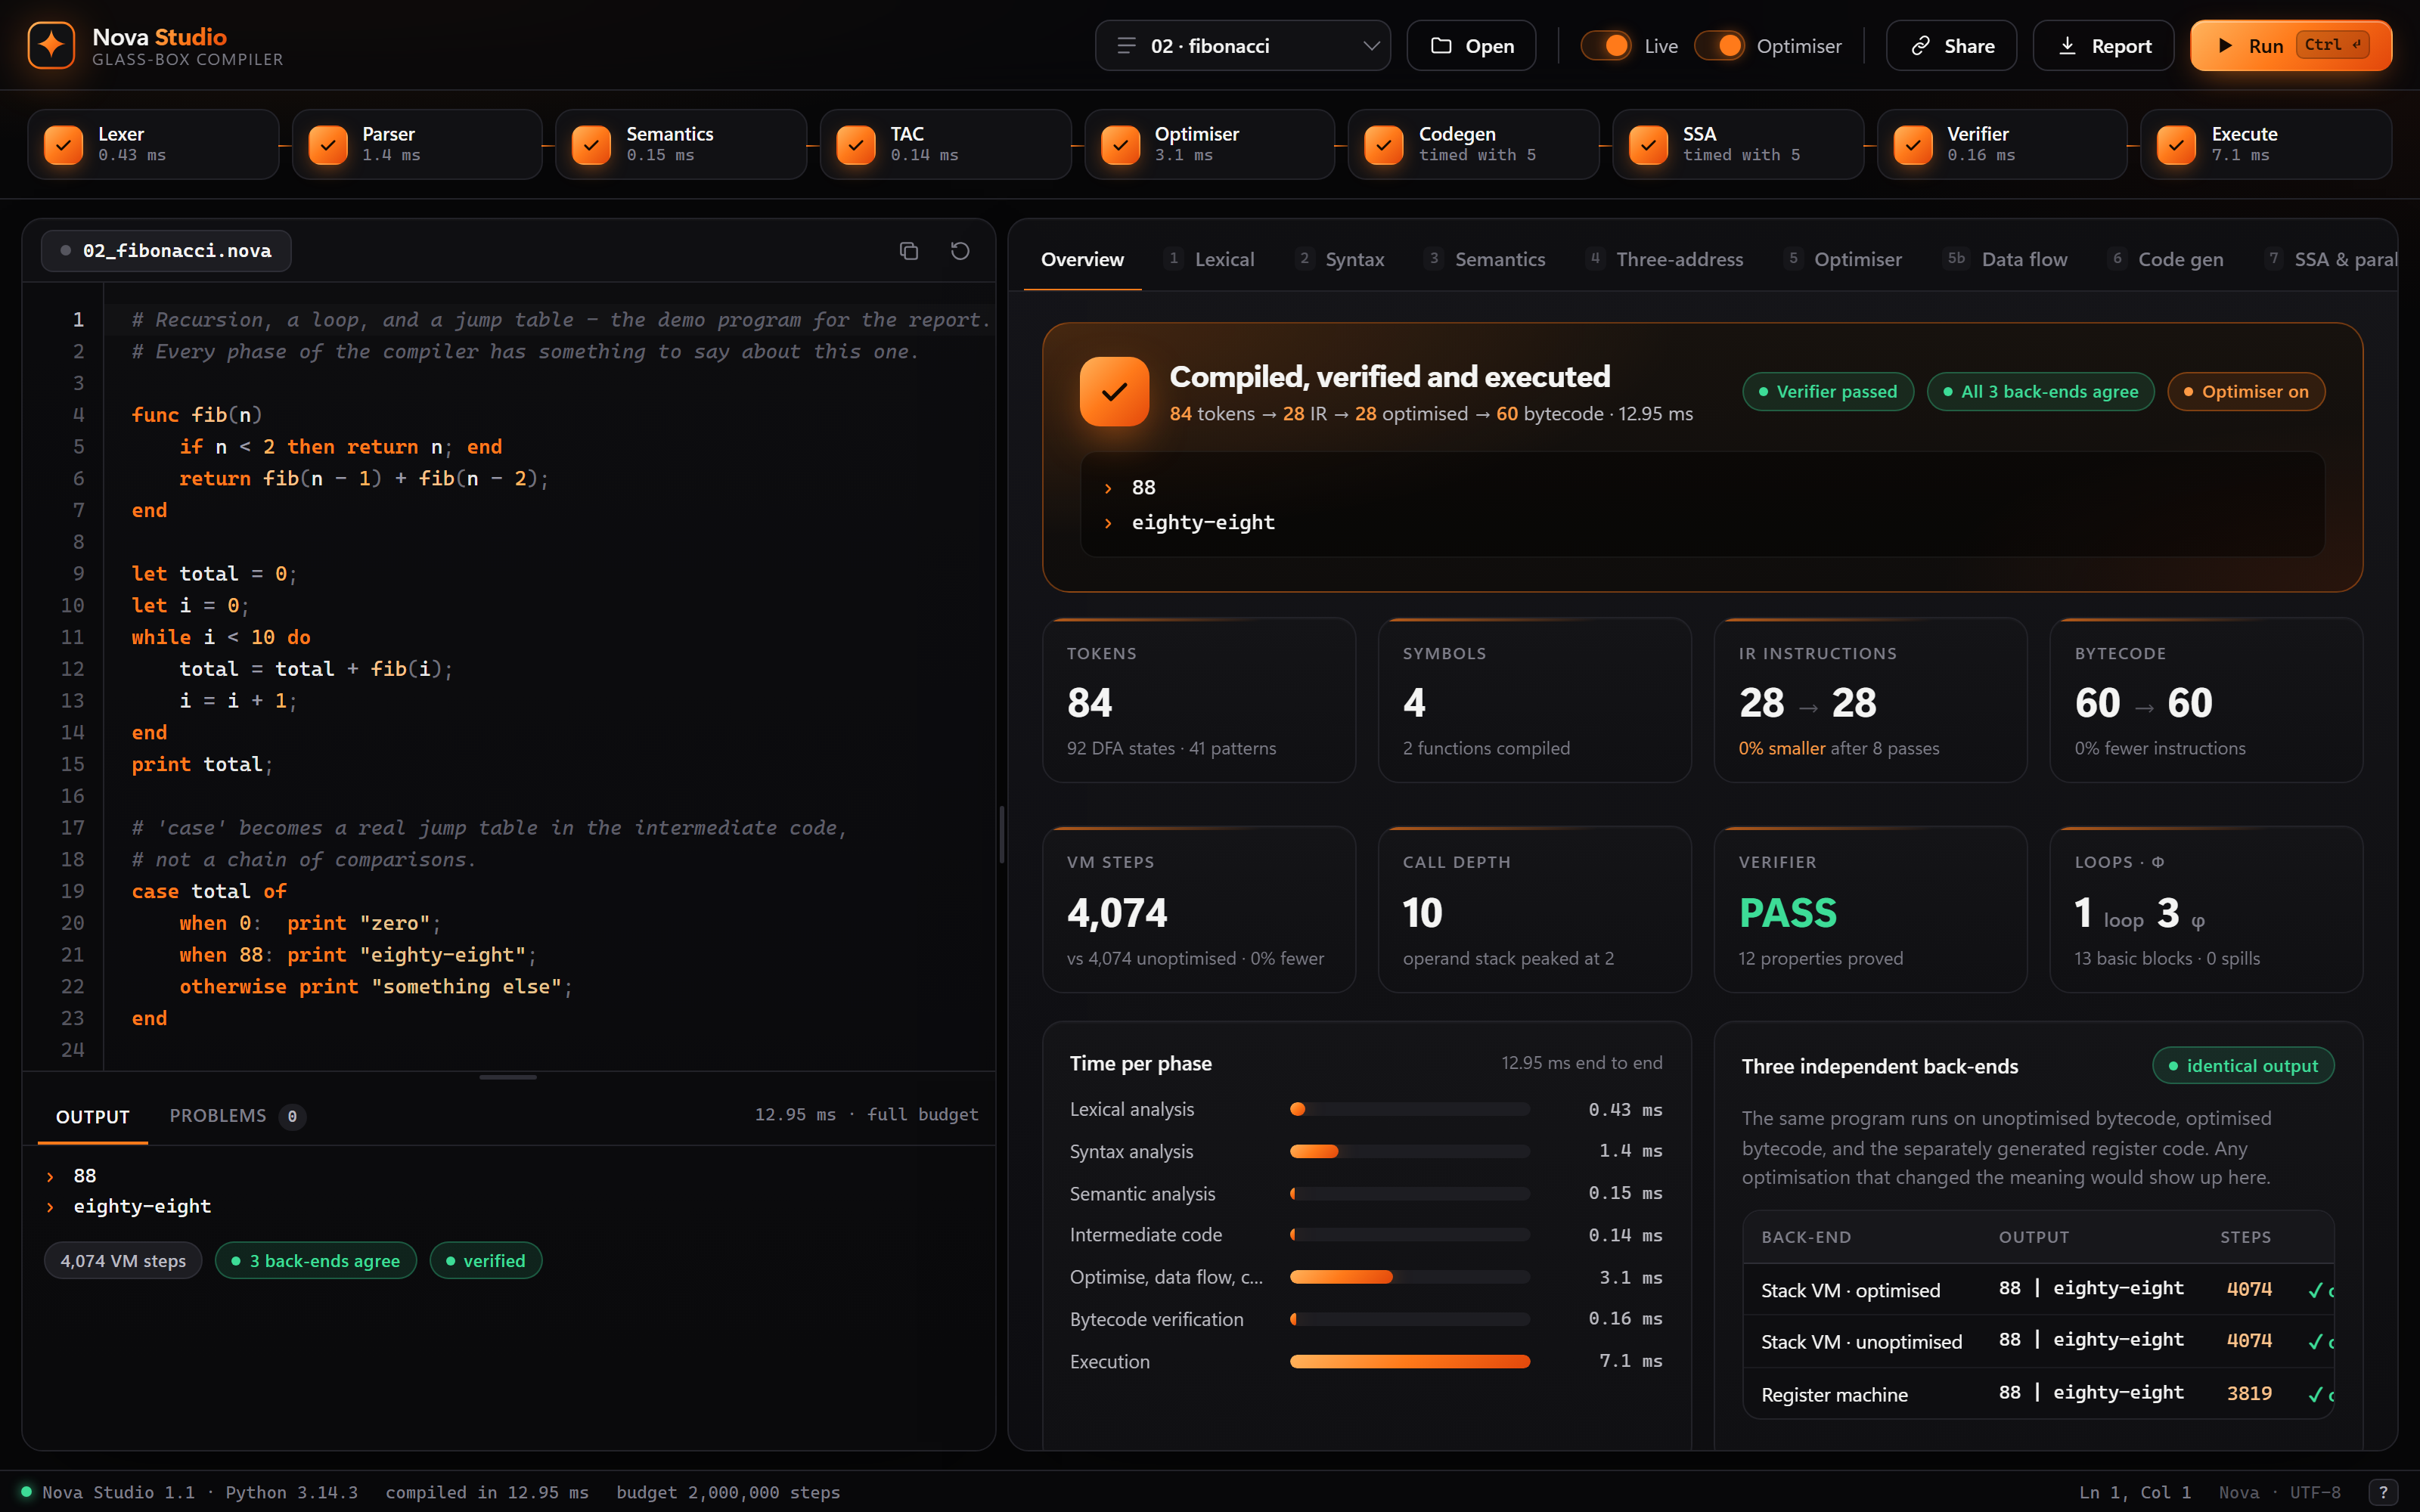
\includegraphics[width=\textwidth]{figures/studio-overview.png}
\caption{Nova Studio compiling \code{02\_fibonacci.nova}. Top: toolbar with example picker, live-compile and optimiser switches, sharing, report download and \emph{Run}. Below it, the pipeline rail shows each of the nine stages with its status and its cost in this compilation. Left: the syntax-highlighted editor and the program output, with a summary of the three back-ends. Right: the inspector's overview of the compilation, including the hero summary, key measurements, per-phase timing and the agreement of the three back-ends. All panels are rendered from one \code{CompileResult}.}
\label{fig:overview}
\end{figure*}

The contributions of this work are:
\begin{itemize}
\item A complete compiler for an original language, implemented in 29 Python modules (7,059 non-blank lines) with no third-party dependencies, covering scanning, parsing, semantic analysis, intermediate code, optimisation, register allocation, SSA construction, dependence analysis, bytecode verification and sandboxed execution (Section~\ref{sec:method}).
\item A side-by-side construction of SLR(1), canonical LR(1) (CLR) and LALR(1) tables for the full language grammar, with a bottom-up parse that independently validates the recursive-descent parser, and a browser for every state and table entry of the LALR(1) automaton (Sections~\ref{sec:syntax} and~\ref{sec:res-front}).
\item A safety pipeline in which an abstract-interpretation verifier proves six properties of all generated bytecode before a resource-bounded virtual machine (VM) executes it, evaluated against eight hand-written hostile programs (Sections~\ref{sec:verify} and~\ref{sec:res-security}).
\item A differential-validation discipline in which unoptimised bytecode, optimised bytecode and separately generated register-machine code must produce identical output for every program (Section~\ref{sec:res-backends}).
\item Nova Studio, a dependency-free local web application that recompiles as the user types and renders every phase as an interactive instrument, together with a security model for a localhost development server (Section~\ref{sec:studio}).
\item A reproducible evaluation on eleven benchmark programs and a synthetic scaling series: scripts regenerate every number, table and screenshot in this report, and the evaluation itself exposed six latent defects, which we analyse (Section~\ref{sec:results}).
\end{itemize}

The rest of the paper is organised as follows. Section~\ref{sec:lit} reviews the literature that Nova builds on and identifies the gap it addresses. Section~\ref{sec:method} presents the methodology: the language, the architecture, each phase, the studio and the evaluation protocol. Section~\ref{sec:results} reports and discusses the results, and Section~\ref{sec:conclusion} concludes and outlines future work.

% =============================================================================
\section{Literature Review}
\label{sec:lit}

\subsection{Foundations of Compiler Construction}
The classical organisation of a compiler, and most of the algorithms used in Nova, are presented in the standard texts of Aho~\emph{et~al.}~\cite{aho2006}, Appel and Palsberg~\cite{appel2002}, Cooper and Torczon~\cite{cooper2011} and Muchnick~\cite{muchnick1997}. These texts describe precisely the artefacts that Nova exposes---automata, parse tables, attribute flows, flow graphs and data-flow solutions---but, being books, they present them statically and for small hand-worked examples.

\subsection{Lexical Analysis}
Thompson's construction translates a regular expression into a nondeterministic finite automaton (NFA) that is then determinised~\cite{thompson1968}. McNaughton and Yamada~\cite{mcnaughton1960} and Glushkov~\cite{glushkov1961} instead built an automaton directly from the \emph{positions} of the symbols in an expression; Berry and Sethi~\cite{berry1986} derived the same position automaton from expression derivatives, and Aho~\emph{et~al.} present it as the \emph{direct method} based on the functions nullable, firstpos, lastpos and followpos~\cite{aho2006}. Moore's partition refinement~\cite{moore1956} and Hopcroft's $O(n \log n)$ algorithm~\cite{hopcroft1971} minimise the resulting deterministic finite automaton (DFA). Lex~\cite{lesk1975} packages these constructions behind a specification language.

\subsection{Syntax Analysis}
Knuth introduced LR($k$) parsing~\cite{knuth1965}. DeRemer's SLR($k$)~\cite{deremer1971} and LALR($k$)~\cite{deremer1969} variants made it practical by keeping the LR(0) automaton and refining only the look-aheads, and DeRemer and Pennello~\cite{deremer1982} showed how to compute LALR(1) look-aheads efficiently without building the canonical LR(1) collection. Yacc~\cite{johnson1975} and its successor Bison generate LALR(1) tables and can describe the automaton in a textual report~\cite{bison}; ANTLR~\cite{parr1995} generates top-down predictive parsers. Hand-written recursive-descent parsers with panic-mode recovery remain common in production front ends because they give precise control over diagnostics~\cite{aho2006}.

\subsection{Semantic Analysis}
Knuth's attribute grammars~\cite{knuth1968} formalised syntax-directed translation with inherited and synthesised attributes. Lewis, Rosenkrantz and Stearns~\cite{lewis1974} characterised the \emph{L-attributed} subclass, whose attributes can be evaluated in a single left-to-right traversal---the property that lets Nova's type checker run in one pass.

\subsection{Optimisation and Data-Flow Analysis}
Allen formalised control-flow analysis over basic blocks, dominators and natural loops~\cite{allen1970}. Kildall unified global optimisations as iterative, lattice-based data-flow analyses~\cite{kildall1973}, and Kam and Ullman established when such iteration converges and how quickly~\cite{kam1976,kam1977}. Cocke~\cite{cocke1970} and Alpern, Wegman and Zadeck~\cite{alpern1988} developed common-subexpression elimination and value numbering; strength reduction~\cite{allen1981} and peephole optimisation~\cite{mckeeman1965} complete the classical repertoire. Cytron~\emph{et~al.}~\cite{cytron1991} showed how to construct static single assignment (SSA) form efficiently by placing $\phi$-functions on iterated dominance frontiers, building on fast dominator algorithms~\cite{lengauer1979,cooper2001}; SSA in turn simplifies sparse analyses such as conditional constant propagation~\cite{wegman1991}.

\subsection{Code Generation and Register Allocation}
Register allocation by graph colouring~\cite{chaitin1982} and by linear scan~\cite{poletto1999} dominates production compilers. The simple code generator taught in compiler courses instead allocates registers within a basic block using \emph{next-use} information~\cite{aho2006}, spilling the value whose next use is furthest away---Belady's optimal replacement rule~\cite{belady1966} applied to registers. LLVM~\cite{lattner2004} popularised a typed, SSA-based intermediate representation that front ends can emit as plain text.

\subsection{Dependence Analysis and Parallelisation}
Allen and Kennedy~\cite{allen1987,allen2001} and Wolfe~\cite{wolfe1996} developed the dependence analysis that underpins vectorisation and loop restructuring; Kennedy and McKinley~\cite{kennedy1993} used it to drive loop fusion and distribution. OpenMP~\cite{openmp2021} exposes the resulting parallel-loop and reduction patterns to programmers.

\subsection{Code Verification and Sandboxing}
Abstract interpretation~\cite{cousot1977} provides the theory for proving program properties by computing over abstract domains. The JVM applies it to bytecode: every class is verified for type and stack safety before execution~\cite{lindholm2014,leroy2003}. Proof-carrying code~\cite{necula1997} and software fault isolation~\cite{wahbe1993} are alternative routes to running untrusted code safely, and WebAssembly validation~\cite{haas2017} and the Linux eBPF verifier~\cite{gershuni2019} are their modern descendants. Nova's verifier is a small instance of the JVM approach, complemented by resource limits enforced at run time.

\subsection{Compiler Correctness}
CompCert~\cite{leroy2009} proves a compiler correct once and for all; translation validation~\cite{pnueli1998} checks each individual compilation instead; differential testing~\cite{mckeeman1998,yang2011} compares the behaviour of independent implementations on the same input. Nova adopts the lightweight end of this spectrum, comparing three back-ends on every program it compiles.

\subsection{Program Visualisation and Educational Compilers}
A meta-study of algorithm visualisation found that the \emph{form} of engagement, not the quality of the graphics, predicts learning: visualisations that learners control, predict and respond to outperform those they only watch~\cite{hundhausen2002}. Sorva~\emph{et~al.}~\cite{sorva2013} reviewed program-visualisation systems for introductory programming and reached the same conclusion, and Guo's Online Python Tutor~\cite{guo2013} showed that a stepping debugger that draws the run-time state is effective at scale. Graph-drawing research supplies the layouts such tools need: Reingold and Tilford's tidy tree layout~\cite{reingold1981} and Sugiyama's layered layout for directed graphs~\cite{sugiyama1981}.

COOL~\cite{aiken1996} and ChocoPy~\cite{padhye2019} are languages designed for compiler courses: students implement phases against a reference compiler, which teaches construction but does not visualise the reference compiler's internals. JFLAP~\cite{rodger2006} animates automata and LL(1) and SLR(1) parsing for formal-language courses but stops before semantic analysis. Compiler Explorer~\cite{godbolt2020} shows interactively the assembly and intermediate code that production compilers generate, but not the front-end artefacts or the analyses that justify each transformation.

\subsection{Research Gap}
Table~\ref{tab:compare} compares these tool families with Nova. To our knowledge, no existing tool lets a learner follow a single program from regular-expression automata through LR tables, attribute flow, data-flow fixed points, register allocation and SSA to verified, sandboxed execution in one live environment, while cross-checking each step and letting the learner drive every instrument. That gap motivates Nova.

\begin{table}[!t]
\caption{Capabilities of Existing Tool Families and Nova}
\label{tab:compare}
\centering
\scriptsize
\setlength{\tabcolsep}{3pt}
\begin{tabular*}{\columnwidth}{@{\extracolsep{\fill}}L{2.95cm}ccccc@{}}
\toprule
Capability & \makecell{GCC/\\LLVM} & \makecell{Bison/\\ANTLR} & JFLAP & CE$^{a}$ & Nova \\
\midrule
Regex $\to$ automaton construction & \nonec & \nonec & \fullc & \nonec & \fullc \\
Scanner trace for a chosen token & \nonec & \nonec & \halfc & \nonec & \fullc \\
LR table construction and comparison & \nonec & \halfc & \halfc & \nonec & \fullc \\
LR automaton browser, parse replay & \nonec & \halfc & \halfc & \nonec & \fullc \\
Annotated tree / attribute flow & \halfc & \nonec & \nonec & \halfc & \fullc \\
IR and per-pass optimisation effects & \halfc & \nonec & \nonec & \fullc & \fullc \\
Data-flow fixed-point iteration & \nonec & \nonec & \nonec & \nonec & \fullc \\
Register-allocation decisions & \halfc & \nonec & \nonec & \halfc & \fullc \\
SSA, dominator tree, frontiers & \halfc & \nonec & \nonec & \halfc & \fullc \\
Bytecode verification and sandbox & \nonec & \nonec & \nonec & \nonec & \fullc \\
VM stepping with activation records & \nonec & \nonec & \nonec & \nonec & \fullc \\
Independent cross-checking & \nonec & \nonec & \nonec & \halfc & \fullc \\
All phases of one program, live & \nonec & \nonec & \nonec & \halfc & \fullc \\
Offline, no third-party packages & \fullc & \fullc & \halfc & \halfc & \fullc \\
\bottomrule
\end{tabular*}
\par\vspace{0pt}
\parbox{\columnwidth}{\scriptsize \fullc\ supported; \halfc\ partial, textual or limited; \nonec\ not supported; based on each tool's documented features. $^{a}$Compiler Explorer.}
\end{table}

% =============================================================================
\section{Methodology}
\label{sec:method}

\subsection{Research Approach and Design Principles}
Nova was developed as design-science research: an artefact is built against explicit requirements and then evaluated empirically. The requirements come from the eight modules of the Compiler Design syllabus that the project addresses (Table~\ref{tab:syllabus}) and from five design principles:
\begin{enumerate}
\item \emph{Glass box.} No phase discards its working. The scanner keeps its syntax tree, followpos table, both automata and, for every token, the DFA states it walked; the parsers keep their item sets, tables and traces; the optimiser records the code after every pass; each data-flow analysis records every iteration; the VM records its trace, including the locals of the current frame at every step. One \code{CompileResult} object holds all of it.
\item \emph{One pipeline, many views.} The command-line interface, the desktop viewer, the HTML report and Nova Studio all render the same \code{CompileResult}, so they cannot disagree.
\item \emph{Trust nothing that can be checked.} Two parsers accept the same token stream, three back-ends execute every program, and a verifier proves the bytecode safe before it runs.
\item \emph{Measure, do not assert.} Every statistic in the user interface, and in this paper, is produced by the compiler or by the scripts in \code{report/tools}.
\item \emph{Zero dependencies.} Only the Python standard library is used, so the tool runs on any machine with Python by double-clicking a launcher; the studio's page is plain HTML, CSS and JavaScript with no framework and no build step.
\end{enumerate}

\begin{table}[!t]
\caption{Syllabus Modules and Their Implementation}
\label{tab:syllabus}
\centering
\footnotesize
\setlength{\tabcolsep}{3pt}
\renewcommand{\arraystretch}{1.08}
\begin{tabular}{@{}l L{3.3cm} L{2.3cm}@{}}
\toprule
Module & Techniques implemented & Source modules \\
\midrule
M1 Lexical & regex $\to$ DFA (direct method), Moore minimisation, maximal munch, per-token scanner trace; LLVM IR & \code{regexdfa}, \code{lexer}, \code{llvmir} \\
M2 Syntax & FIRST/FOLLOW, LL(1), left recursion, SLR/CLR/LALR, automaton browser, recursive descent, panic mode, parse replay & \code{grammar}, \code{lr}, \code{parser} \\
M3 Semantics & scoped symbol table, L-attributed SDD, type checking, drawn annotated tree & \code{semantic}, \code{ast\_nodes} \\
M4 Intermediate & three-address code, backpatching, jumping code, jump tables & \code{tac} \\
M5 Optimisation & blocks, CFG, DAG/LVN, eight passes, four data-flow analyses drawn on the graph & \code{cfg}, \code{dag}, \code{dataflow}, \code{optimizer} \\
M6 Code gen. & next use, register allocation with a register timeline, activation records, two executable targets & \code{codegen}, \code{regvm}, \code{bytecode}, \code{vm} \\
M7 SSA, parallel & dominator tree, dominance frontiers, $\phi$ placement, dependence analysis & \code{ssa}, \code{parallel} \\
M8 Contemporary & bytecode verification, sandboxing, VM stepper, hostile code & \code{verifier}, \code{vm}, \code{attacks} \\
\bottomrule
\end{tabular}
\end{table}

\subsection{The Nova Language}
Nova is a small imperative language whose syntax is deliberately not C-like (Fig.~\ref{fig:listing}). A program is a sequence of function declarations and statements; statements are \code{let} declarations, assignments, \code{if}--\code{then}--\code{else}--\code{end}, \code{while}--\code{do}--\code{end}, \code{case}--\code{of}--\code{when}--\code{otherwise}--\code{end}, \code{print}, \code{return} and call statements. Expressions follow the usual precedence chain from \code{or} through \code{and}, equality, relational, additive and multiplicative operators to unary \code{-} and \code{not}. The types \code{int}, \code{bool} and \code{str} are inferred and checked; \code{+} also concatenates two strings. Functions take integer parameters and may be recursive, and scopes nest and shadow. The lexical specification has 41 token patterns (19 keywords, literals, identifiers, operators, whitespace and comments), and the grammar has 58 productions over 39 terminals and 20 non-terminals.

\begin{figure}[!t]
\begin{lstlisting}
func fib(n)
    if n < 2 then return n; end
    return fib(n - 1) + fib(n - 2);
end

let total = 0;
let i = 0;
while i < 10 do
    total = total + fib(i);
    i = i + 1;
end
print total;

case total of
    when 0:  print "zero";
    when 88: print "eighty-eight";
    otherwise print "something else";
end
\end{lstlisting}
\caption{The Fibonacci benchmark (\code{02\_fibonacci.nova}, comments removed): recursion, a loop and a \code{case} statement that compiles to a jump table. It prints \code{88} and \code{eighty-eight}.}
\label{fig:listing}
\end{figure}

\subsection{System Architecture}
Fig.~\ref{fig:arch} shows the architecture. The driver, \code{pipeline.py}, runs the phases in order and stores every intermediate product in the \code{CompileResult}; phases 1--3 form the front end, which stops compilation if it reports errors. After intermediate-code generation, each function is cut into basic blocks twice: one copy feeds an unoptimised bytecode generator, and the other flows through the optimiser, the register code generator, SSA construction, dependence analysis, the optimised bytecode generator and the LLVM IR emitter. The optimised bytecode must pass the verifier before the sandboxed VM will run it; the unoptimised bytecode and the register code are also executed, and the three outputs are compared. Four front ends render the result.

\begin{figure*}[!t]
\centering
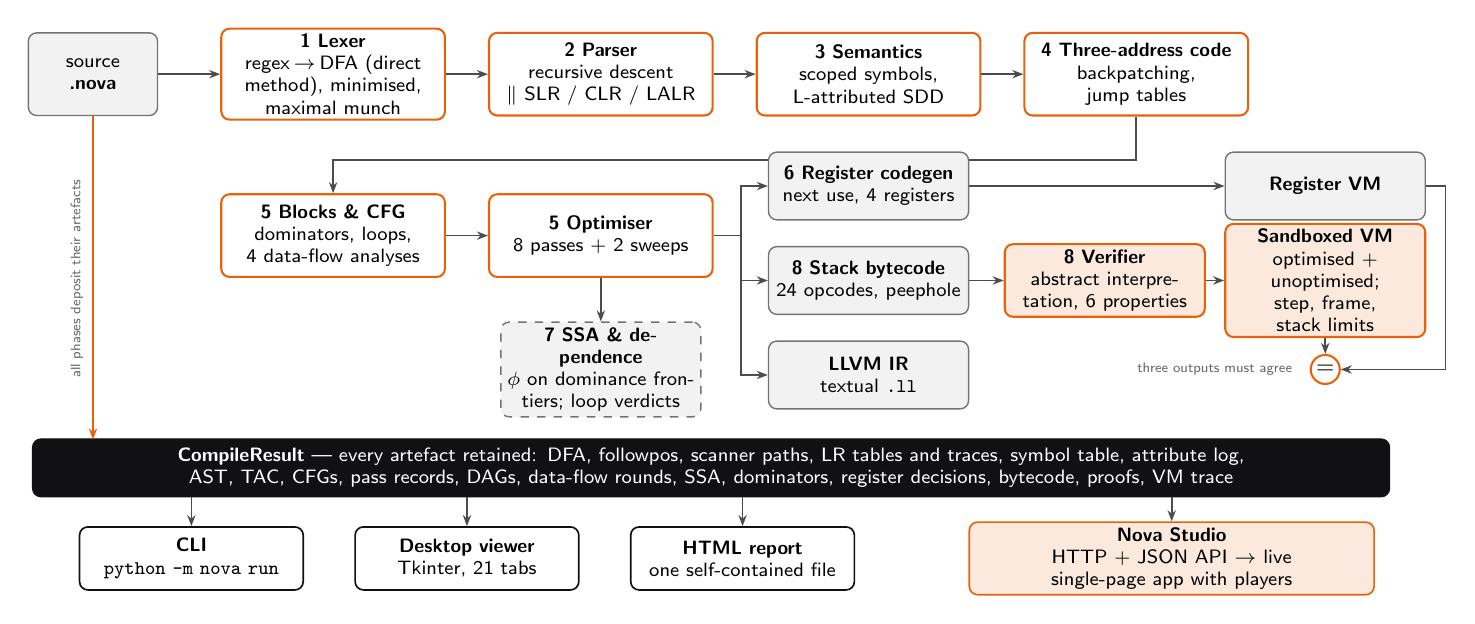
\begin{tikzpicture}[
  font=\scriptsize\sffamily, >={Stealth[length=4pt]},
  phase/.style={draw=novaorange, line width=0.75pt, rounded corners=3pt, fill=white,
    align=center, minimum height=10.5mm, text width=27mm, inner sep=2pt},
  back/.style={draw=black!55, line width=0.5pt, rounded corners=3pt, fill=black!5,
    align=center, minimum height=8.6mm, text width=24mm, inner sep=2pt},
  safe/.style={draw=novaorange, line width=0.75pt, rounded corners=3pt, fill=novaorange!14,
    align=center, minimum height=8.6mm, text width=24mm, inner sep=2pt},
  view/.style={draw=novablack, line width=0.6pt, rounded corners=3pt, fill=white,
    align=center, minimum height=8mm, inner sep=2pt},
  arr/.style={->, draw=black!70, line width=0.6pt},
  note/.style={font=\tiny\sffamily, text=black!60, align=center}]
% ---------------------------------------------------------------- row 1
\node[back, text width=15mm, minimum height=10.5mm] (src) at (0.9,0) {source\\\textbf{.nova}};
\node[phase] (lex) at (3.95,0) {\textbf{1 Lexer}\\regex$\,\to\,$DFA (direct method), minimised, maximal munch};
\node[phase] (par) at (7.35,0) {\textbf{2 Parser}\\recursive descent\\$\parallel$ SLR / CLR / LALR};
\node[phase] (sem) at (10.75,0) {\textbf{3 Semantics}\\scoped symbols,\\L-attributed SDD};
\node[phase] (tac) at (14.15,0) {\textbf{4 Three-address code}\\backpatching,\\jump tables};
\draw[arr] (src) -- (lex);
\draw[arr] (lex) -- (par);
\draw[arr] (par) -- (sem);
\draw[arr] (sem) -- (tac);
% ---------------------------------------------------------------- row 2
\node[phase] (cfg) at (3.95,-2.05) {\textbf{5 Blocks \& CFG}\\dominators, loops,\\4 data-flow analyses};
\node[phase] (opt) at (7.35,-2.05) {\textbf{5 Optimiser}\\8 passes + 2 sweeps};
\node[back, dashed] (ssa) at (7.35,-3.75) {\textbf{7 SSA \& dependence}\\$\phi$ on dominance frontiers; loop verdicts};
\draw[arr] (tac.south) -- ++(0,-0.55) -| (cfg.north);
\draw[arr] (cfg) -- (opt);
\draw[arr] (opt) -- (ssa);
\node[back] (rcg) at (10.75,-1.42) {\textbf{6 Register codegen}\\next use, 4 registers};
\node[back] (bc)  at (10.75,-2.62) {\textbf{8 Stack bytecode}\\24 opcodes, peephole};
\node[back] (ll)  at (10.75,-3.82) {\textbf{LLVM IR}\\textual \texttt{.ll}};
\node[safe] (ver) at (13.75,-2.62) {\textbf{8 Verifier}\\abstract interpretation, 6 properties};
\node[back] (rvm) at (16.55,-1.42) {\textbf{Register VM}};
\node[safe] (vm)  at (16.55,-2.62) {\textbf{Sandboxed VM}\\optimised + unoptimised;\\step, frame, stack limits};
\draw[arr] (opt.east) -- ++(0.35,0) |- (rcg.west);
\draw[arr] (opt.east) -- ++(0.35,0) |- (bc.west);
\draw[arr] (opt.east) -- ++(0.35,0) |- (ll.west);
\draw[arr] (rcg) -- (rvm);
\draw[arr] (bc) -- (ver);
\draw[arr] (ver) -- (vm);
\node[draw=novaorange, line width=0.75pt, circle, fill=white, inner sep=1.2pt, font=\footnotesize\bfseries]
  (eq) at (16.55,-3.75) {$=$};
\draw[arr] (rvm.east) -- ++(0.25,0) |- (eq.east);
\draw[arr] (vm) -- (eq);
\node[note, anchor=east] at ($(eq.west)+(-0.1,0)$) {three outputs must agree};
% ---------------------------------------------------------------- row 3
\node[draw=novablack, fill=novablack, text=white, rounded corners=3pt, minimum height=7mm,
  text width=17.0cm, font=\scriptsize\sffamily, align=center] (res) at (8.75,-5.0)
  {\textbf{CompileResult} --- every artefact retained: DFA, followpos, scanner paths, LR tables and traces, symbol table,
   attribute log, AST, TAC, CFGs, pass records, DAGs, data-flow rounds, SSA, dominators, register decisions, bytecode, proofs, VM trace};
\draw[arr, line width=0.9pt, draw=novaorange] (0.9,-0.53) -- (0.9,-4.64);
\node[note, rotate=90, anchor=south] at (0.9,-2.6) {all phases deposit their artefacts};
\node[view, text width=27mm] (cli) at (2.15,-6.15) {\textbf{CLI}\\\texttt{python -m nova run}};
\node[view, text width=27mm] (gui) at (5.65,-6.15) {\textbf{Desktop viewer}\\Tkinter, 21 tabs};
\node[view, text width=27mm] (rep) at (9.15,-6.15) {\textbf{HTML report}\\one self-contained file};
\node[view, text width=50mm, fill=novaorange!14, draw=novaorange] (studio) at (14.6,-6.15)
  {\textbf{Nova Studio}\\HTTP + JSON API $\to$ live single-page app with players};
\foreach \n in {cli,gui,rep,studio} \draw[arr] (res.south -| \n.north) -- (\n.north);
\end{tikzpicture}
\caption{Architecture of Nova. Orange-bordered boxes are compiler phases (numbered by syllabus module); grey boxes are back-ends; tinted boxes enforce safety. The optimised path is shown solid; a second, unoptimised copy of each function is compiled to bytecode and executed so that three independent executions can be compared. Every phase deposits its artefacts in a single \code{CompileResult}, which four front ends render.}
\label{fig:arch}
\end{figure*}

\subsection{Lexical Analysis}
\label{sec:lexical}
Each of the 41 token patterns is an extended regular expression. The patterns are combined into a single expression $(r_1\#_1 \mid r_2\#_2 \mid \cdots \mid r_{41}\#_{41})$, in which every end marker $\#_k$ identifies a token kind, and the syntax tree of this expression yields 147 leaf positions. The functions nullable, firstpos and lastpos are computed bottom-up, and followpos is built from the two rules of the direct method~\cite{aho2006}: for every node $n$ and every position $i \in \mathit{lastpos}(c_1)$,
\begin{equation}
\mathit{followpos}(i) \supseteq
\begin{cases}
\mathit{firstpos}(c_2) & \text{if } n = c_1 \cdot c_2,\\
\mathit{firstpos}(c_1) & \text{if } n = c_1^{*}.
\end{cases}
\label{eq:followpos}
\end{equation}
DFA states are sets of positions: the start state is $\mathit{firstpos}(\mathit{root})$, and the transition on input class $a$ from state $S$ is the union of $\mathit{followpos}(p)$ over the positions $p \in S$ that carry $a$. A state that contains several end markers accepts the token with the lowest index, which is how keywords take priority over identifiers. Characters that behave identically are grouped into 37 equivalence classes, which become the DFA's columns. The automaton is minimised by Moore's partition refinement~\cite{moore1956}, starting from one block per token kind plus one for non-accepting states.

Scanning simulates the minimised DFA with the maximal-munch rule: the scanner keeps reading while a transition exists, remembers the last accepting state it passed, and when it is stuck gives back whatever it read beyond that point. Python's \code{re} module is never imported. Each token records the list of DFA states it walked through and how many characters were read ahead and returned, which is what the studio's \emph{scanner trace} draws (Fig.~\ref{fig:scanner}): the chain of states for the chosen token, the character on every edge, the accepting token of every accepting state, and the final state highlighted. Fig.~\ref{fig:lexical} shows the summary view and the token stream, and Fig.~\ref{fig:dfatable} the minimised automaton itself. The inputs to that construction are inspectable too: the 41 extended regular expressions in priority order (Fig.~\ref{fig:tokenspecs}) and the followpos table that the direct method computes from them (Fig.~\ref{fig:followpos}); and so is its output, the token table with each token's position and attribute value (Fig.~\ref{fig:tokentable}). The followpos rows for the keyword \code{let} (positions 7--10) show the mechanism in miniature: each letter's only follower is the next letter, and the follower of the final \code{t} (position 9) is the end marker \code{\#LET} at position 10, which is what makes the DFA state reached after \code{let} accept the token \code{LET}.

\begin{figure}[!t]
\centering
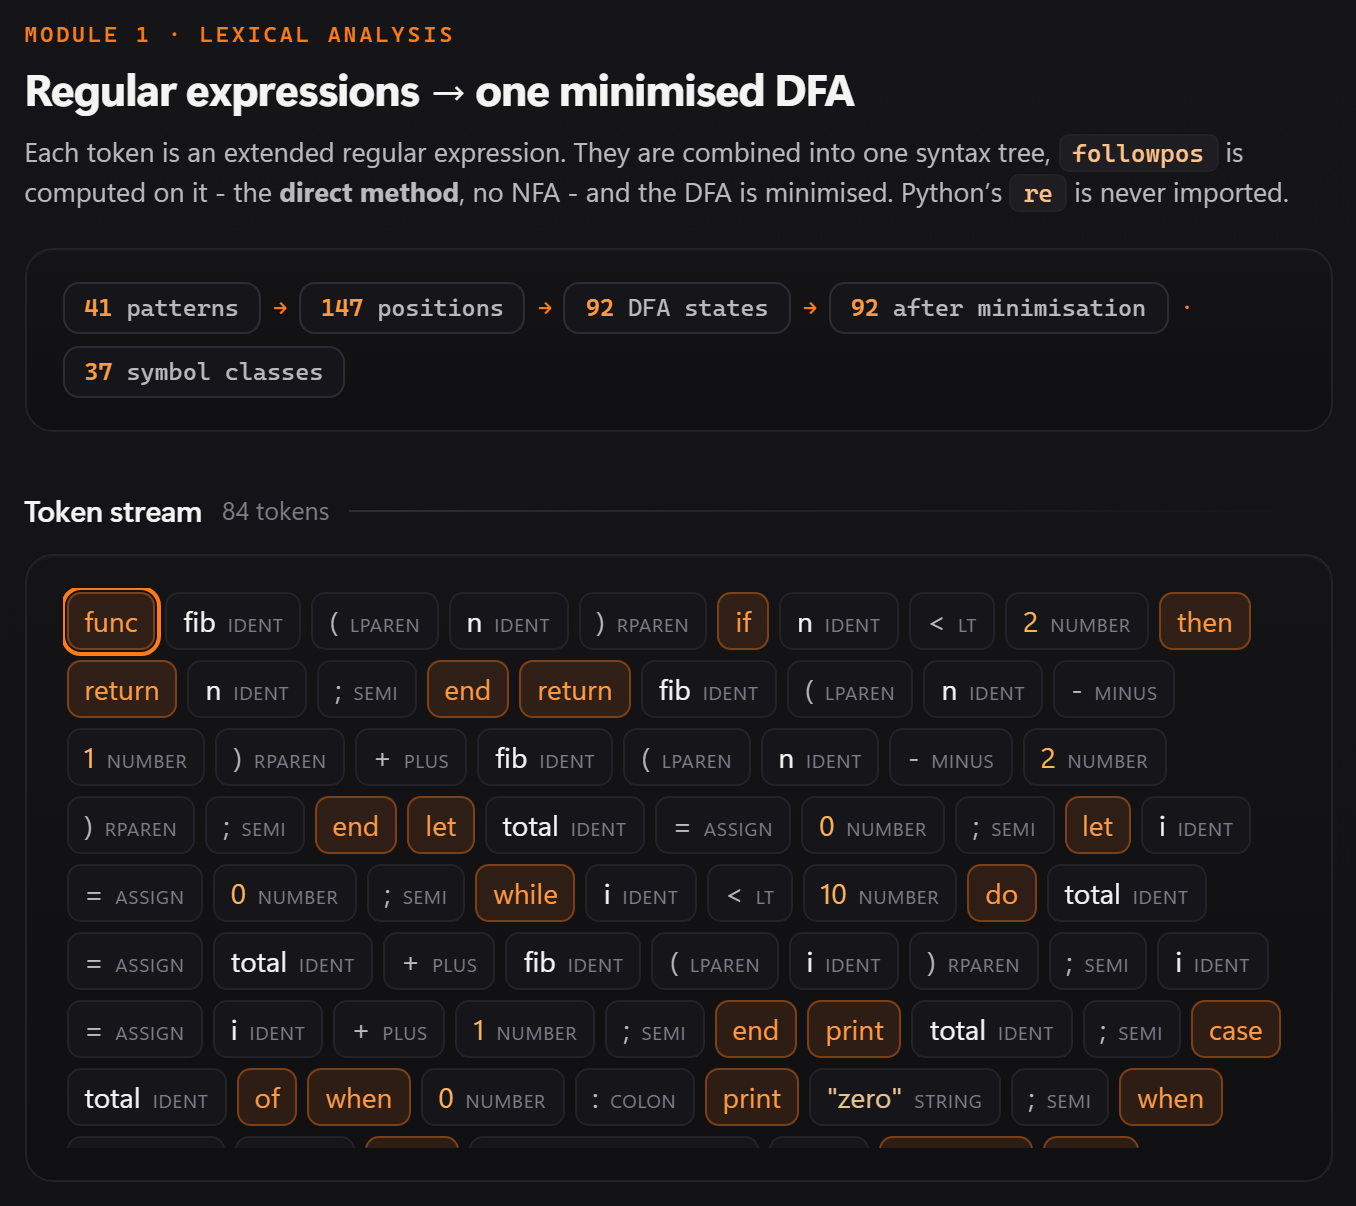
\includegraphics[width=\columnwidth]{figures/view-lexical.png}
\caption{Lexical view: 41 patterns yield 147 positions and a 92-state DFA (already minimal) over 37 symbol classes. Below, the token stream of the Fibonacci program, with keywords highlighted in orange and each token's kind shown in small capitals. Every token is a button that opens the scanner trace of Fig.~\ref{fig:scanner}.}
\label{fig:lexical}
\end{figure}

\begin{figure}[!t]
\centering
\subfloat[The keyword \code{func}: four transitions, three of them through states that accept \code{IDENT}, ending in state 74, which accepts \code{FUNC}.]{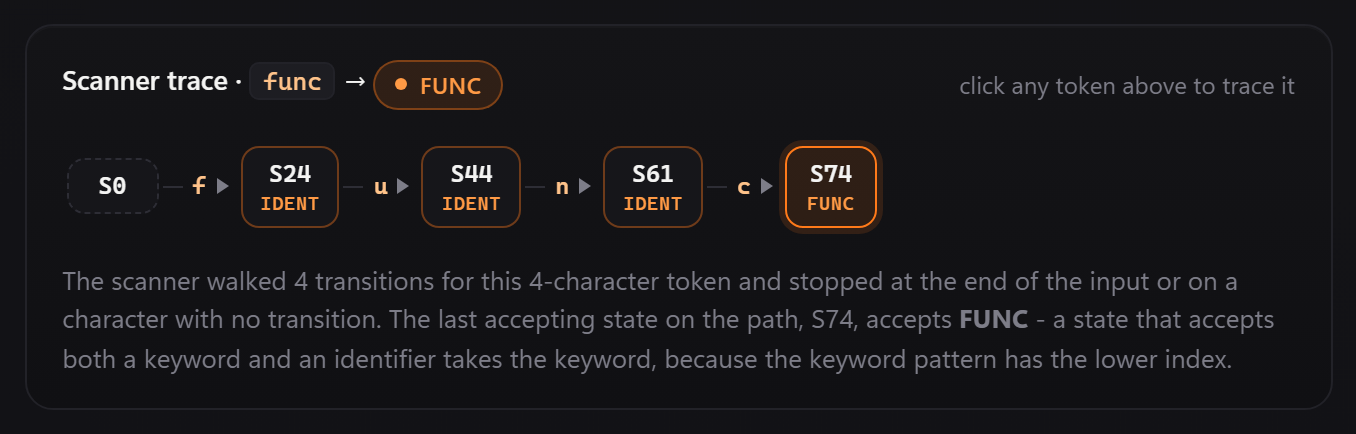
\includegraphics[width=\columnwidth]{figures/scanner-trace.png}\label{fig:scanner-func}}\\[4pt]
\subfloat[The identifier \code{total}: after the first letter the scanner stays in state 19, the generic identifier state, for the remaining four characters.]{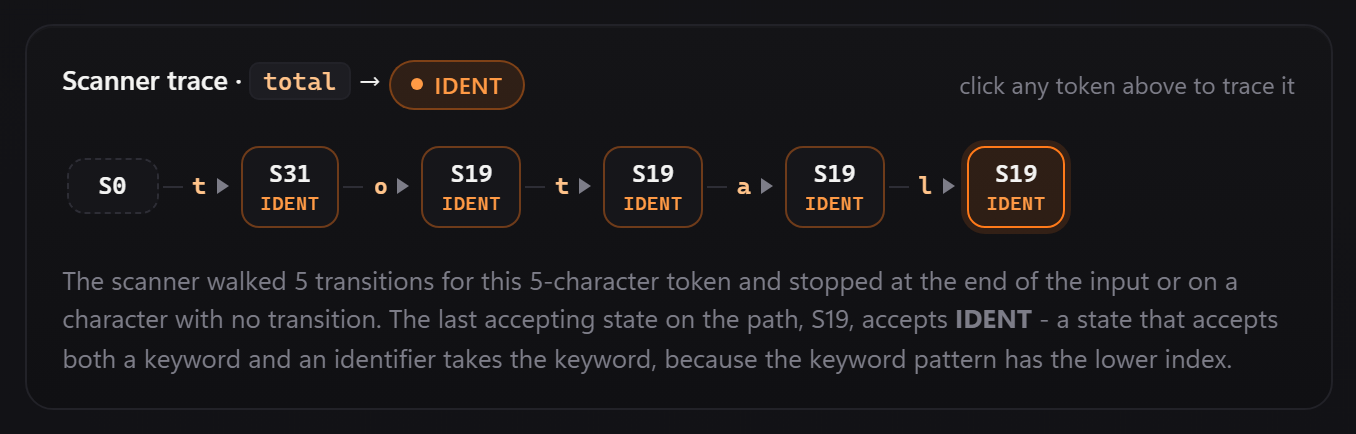
\includegraphics[width=\columnwidth]{figures/scanner-trace-ident.png}\label{fig:scanner-ident}}
\caption{The scanner trace. Clicking a token in the stream of Fig.~\ref{fig:lexical} shows the exact path the minimised DFA took for it, with the input character on each edge and the token each accepting state accepts. The explanation below the chain states why scanning stopped and why the final state's token was chosen.}
\label{fig:scanner}
\end{figure}

\begin{figure}[!t]
\centering
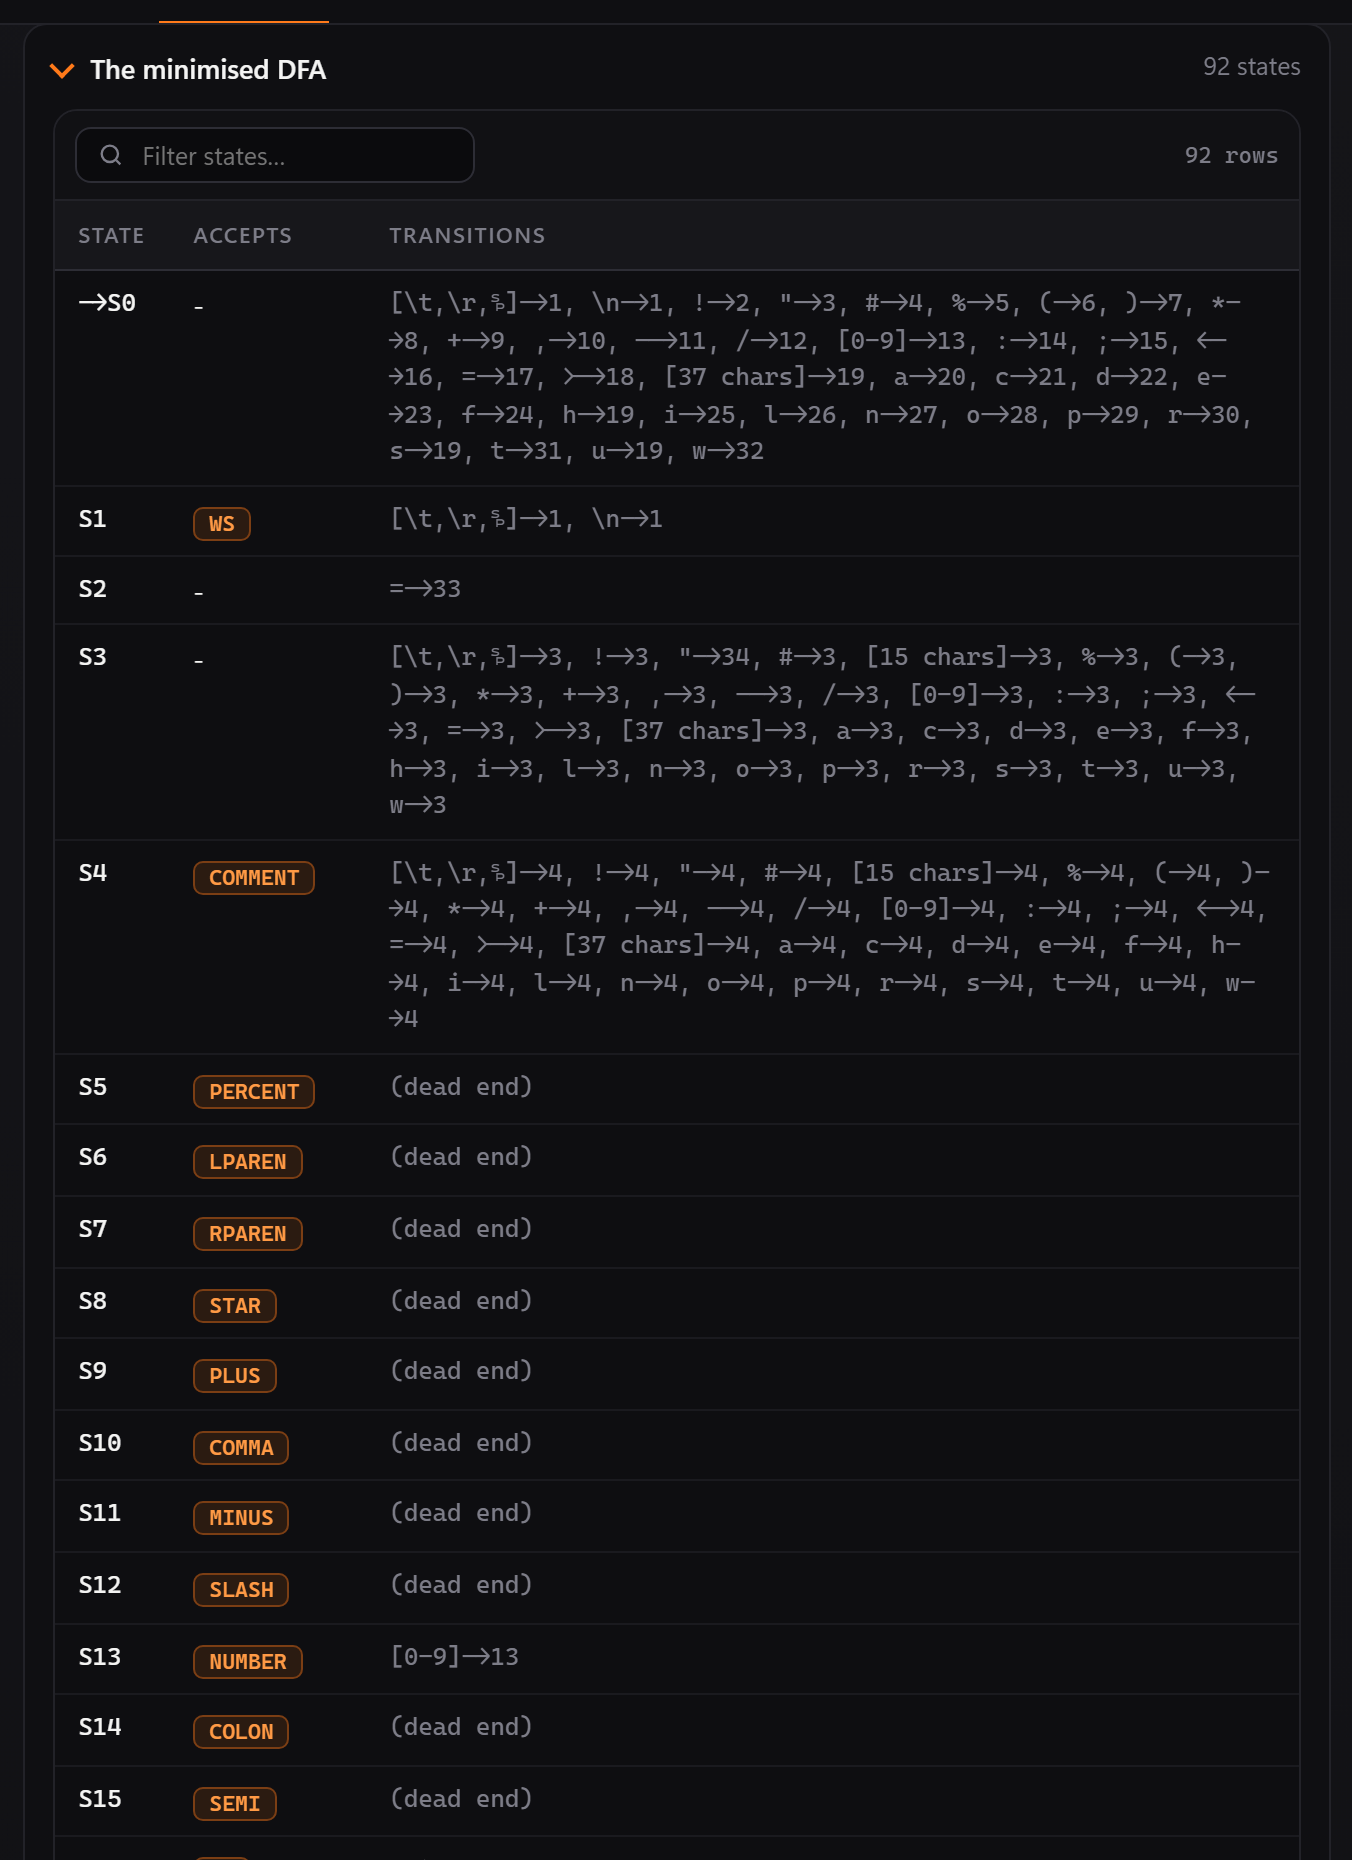
\includegraphics[width=\columnwidth]{figures/dfa-table.png}
\caption{The first sixteen states of the minimised DFA as the studio lists them: the start state \code{S0} with one transition per symbol class, the whitespace and comment loops, single-character operator states that are dead ends, and the \code{NUMBER} state that loops on digits.}
\label{fig:dfatable}
\end{figure}

\begin{figure}[!t]
\centering
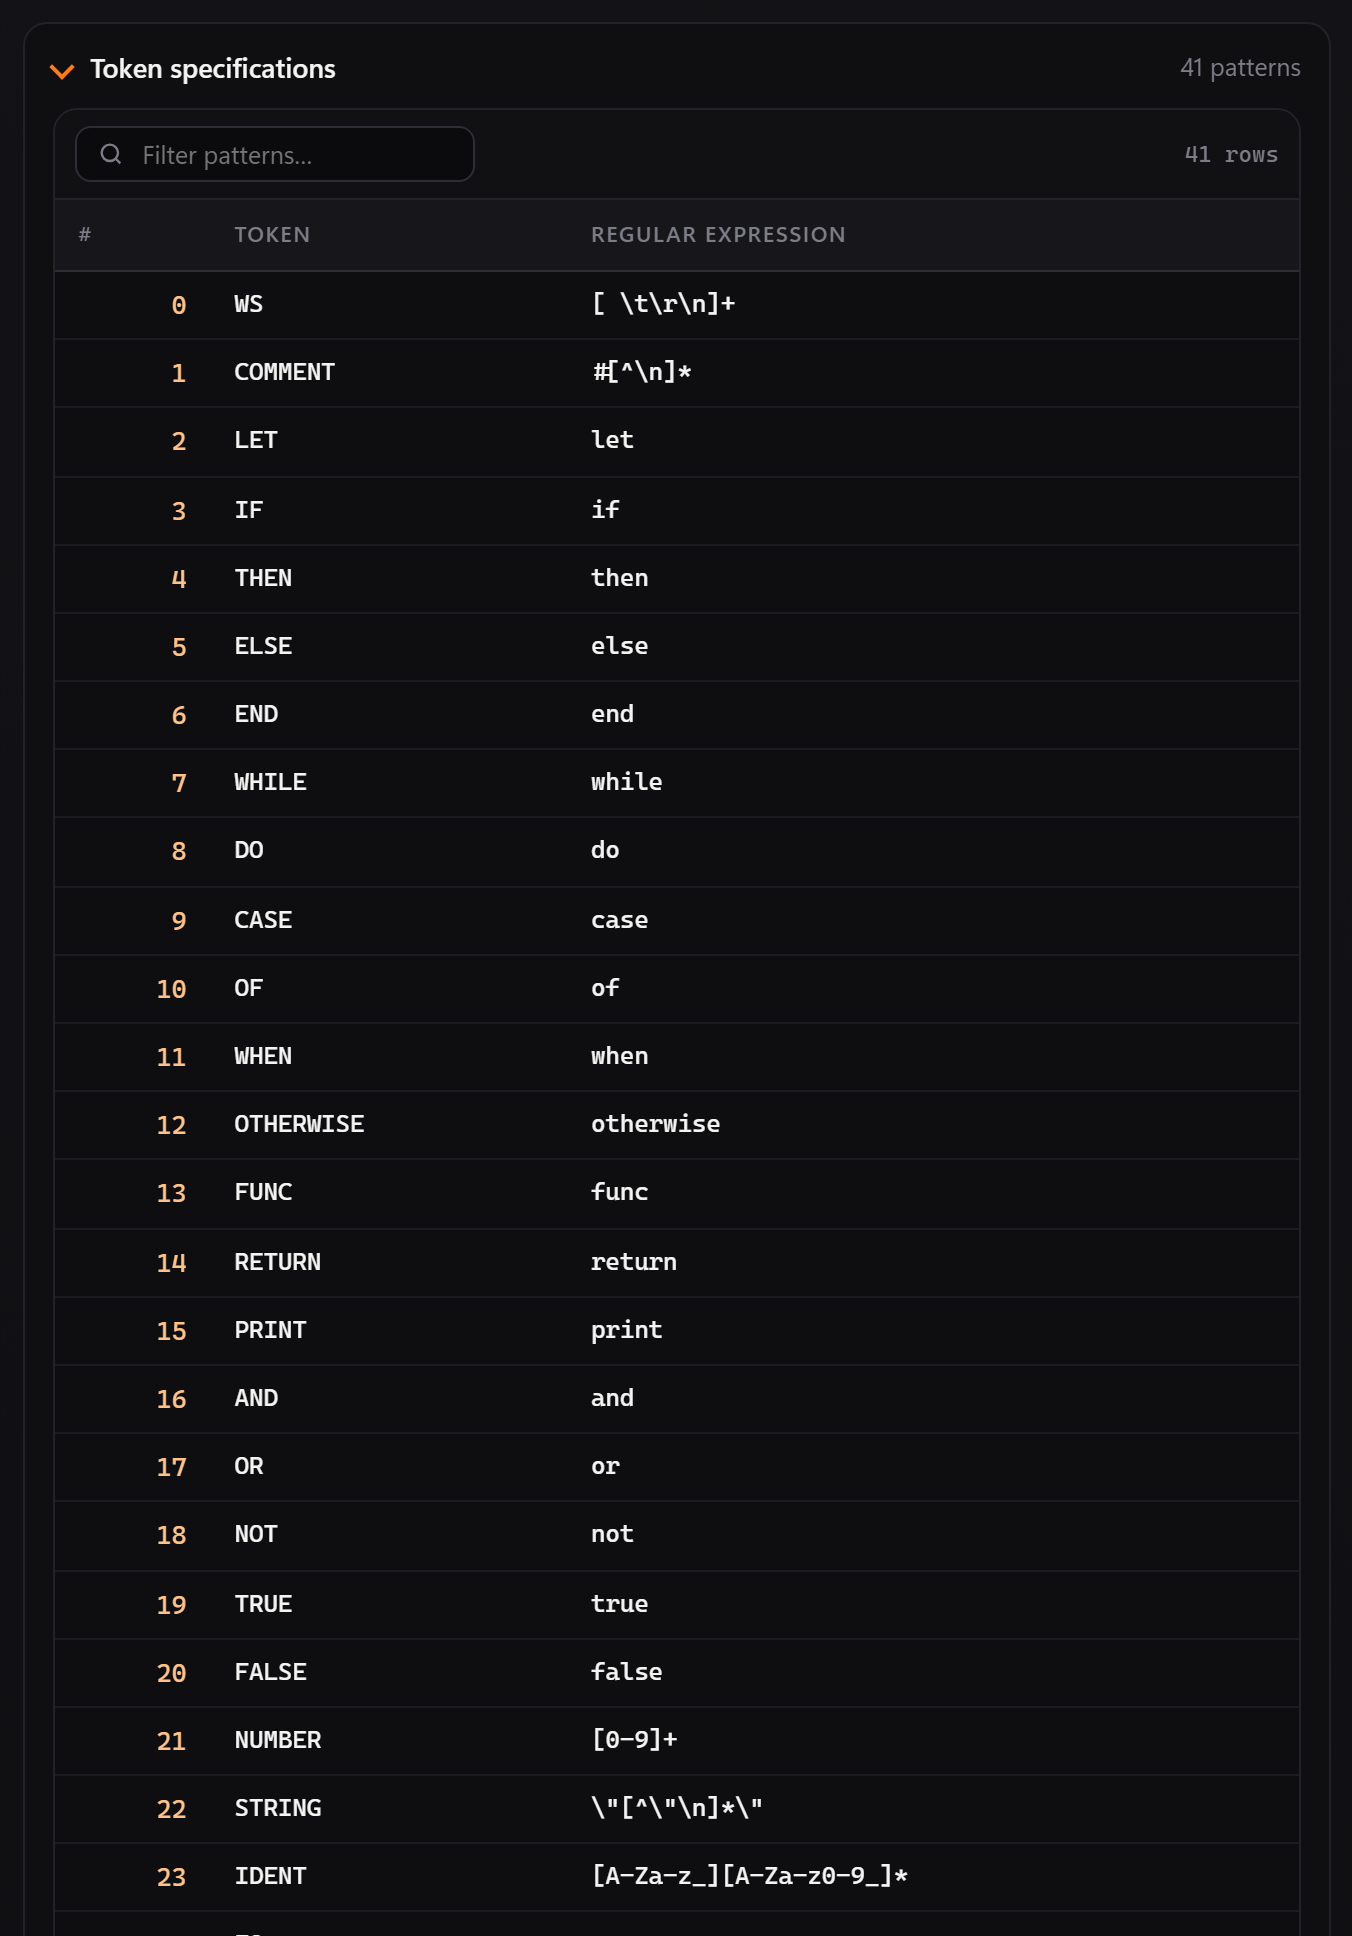
\includegraphics[width=0.92\columnwidth]{figures/token-specs.png}
\caption{The token specification as the studio lists it: the first 24 of the 41 extended regular expressions, in priority order. Whitespace and comments come first, then the 19 keywords, each a literal string, and only then the general patterns for numbers, strings and identifiers, so that a keyword wins any tie with \code{IDENT}.}
\label{fig:tokenspecs}
\end{figure}

\begin{figure}[!t]
\centering
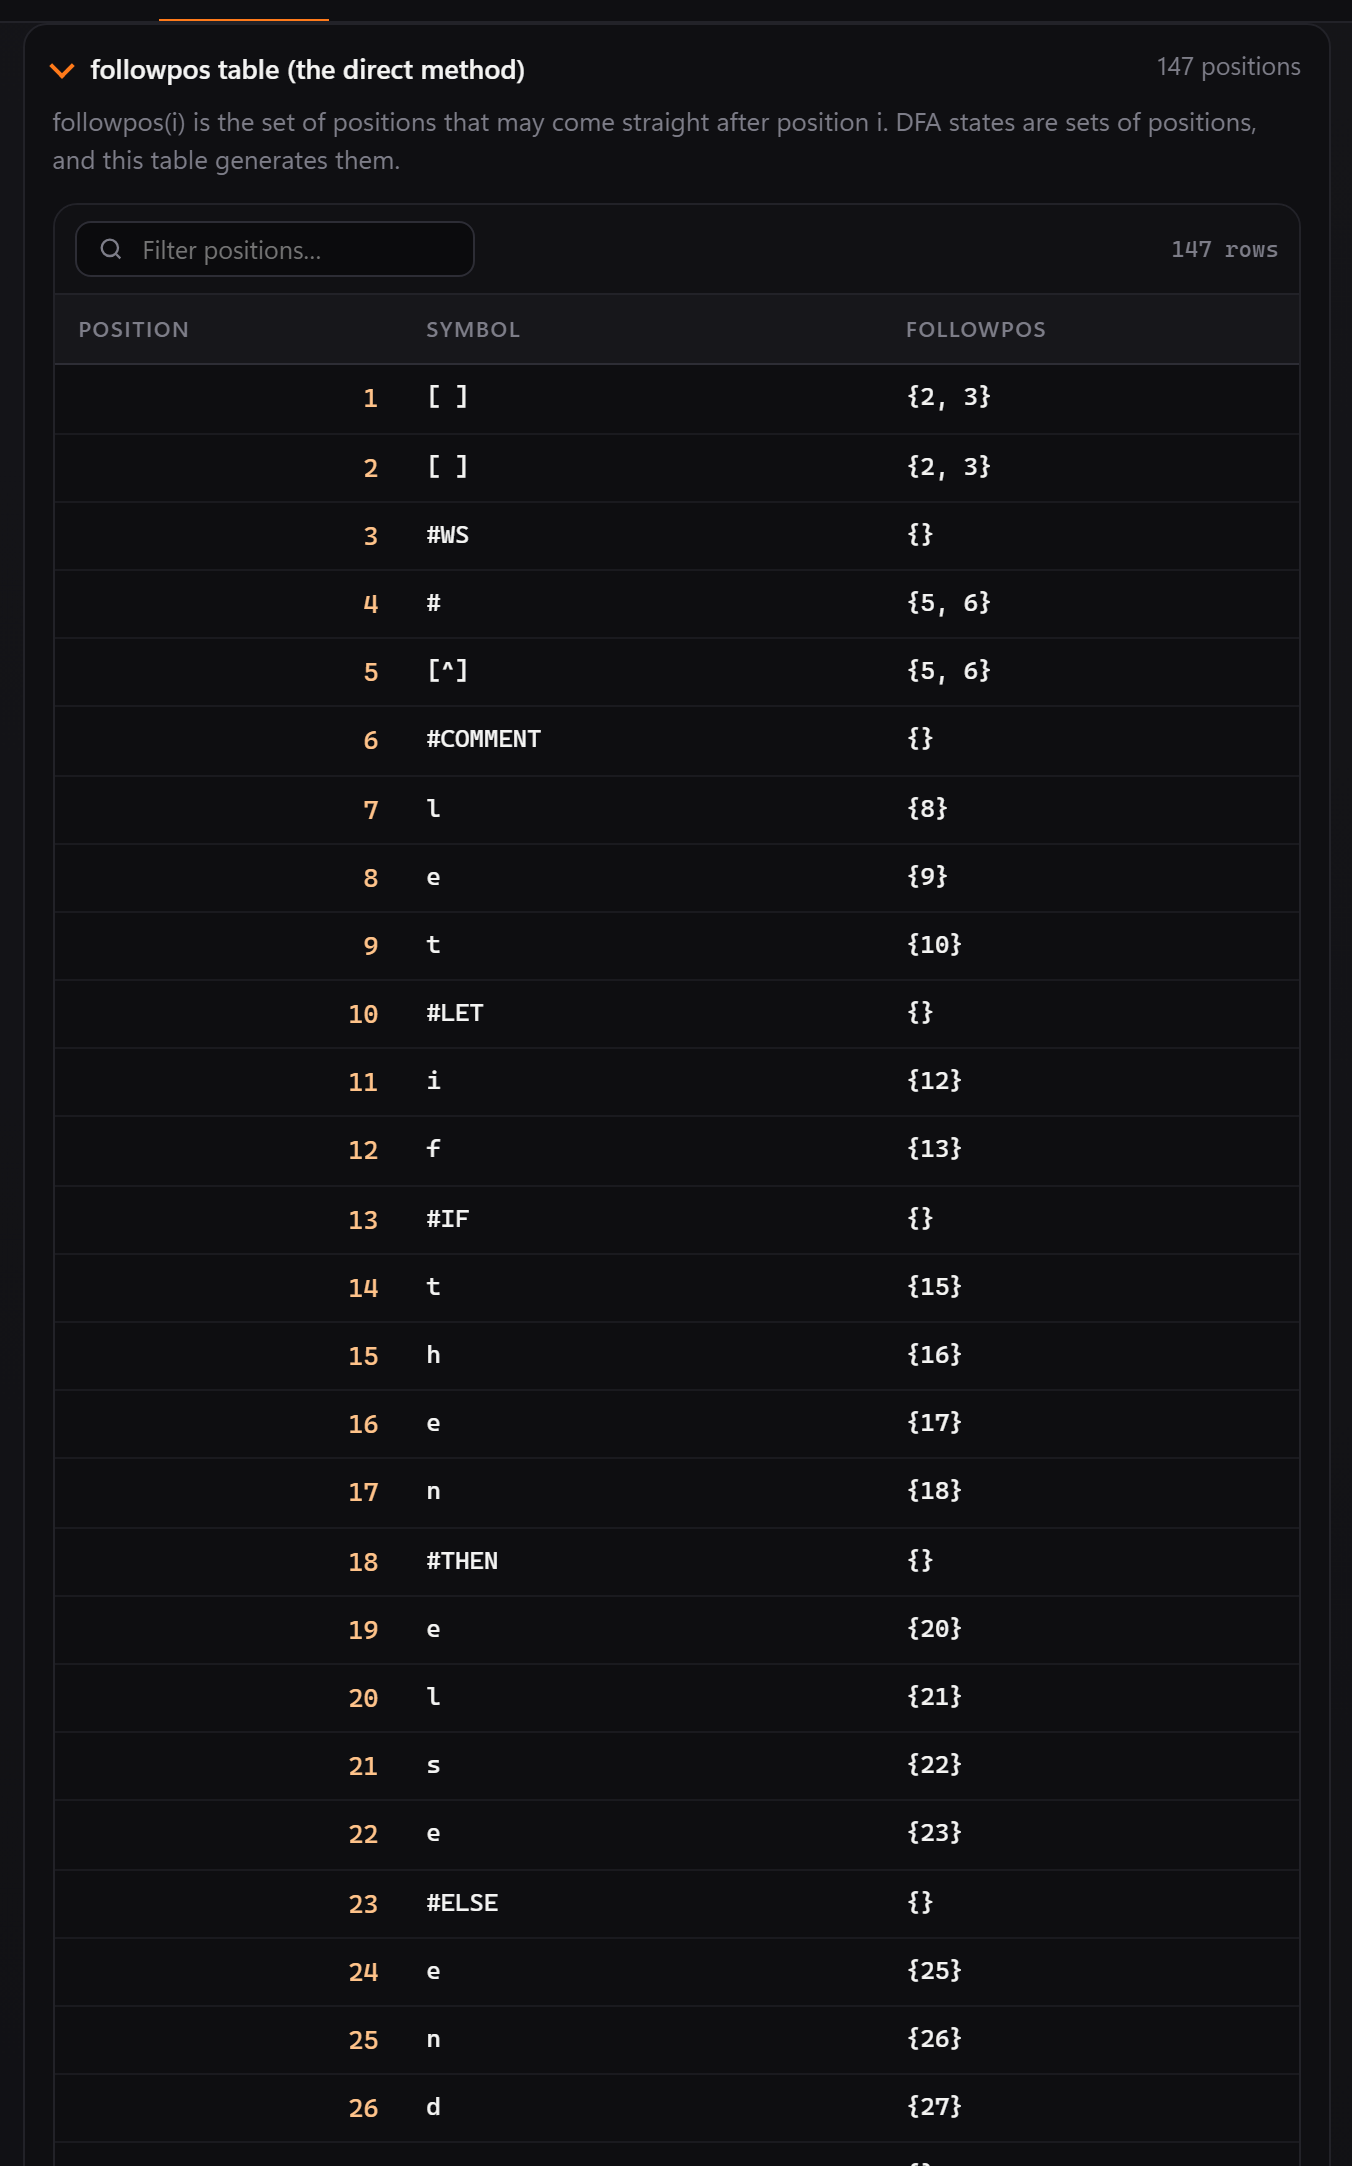
\includegraphics[width=0.92\columnwidth]{figures/followpos.png}
\caption{The followpos table of the direct method, positions 1--26 of 147. Positions 1 and 2 are the two character classes of the whitespace pattern, each followed by both of them (the Kleene star) and by the end marker \code{\#WS} at position 3; the keywords \code{let}, \code{if}, \code{then} and \code{else} are chains of single letters ending in their end markers.}
\label{fig:followpos}
\end{figure}

\begin{figure}[!t]
\centering
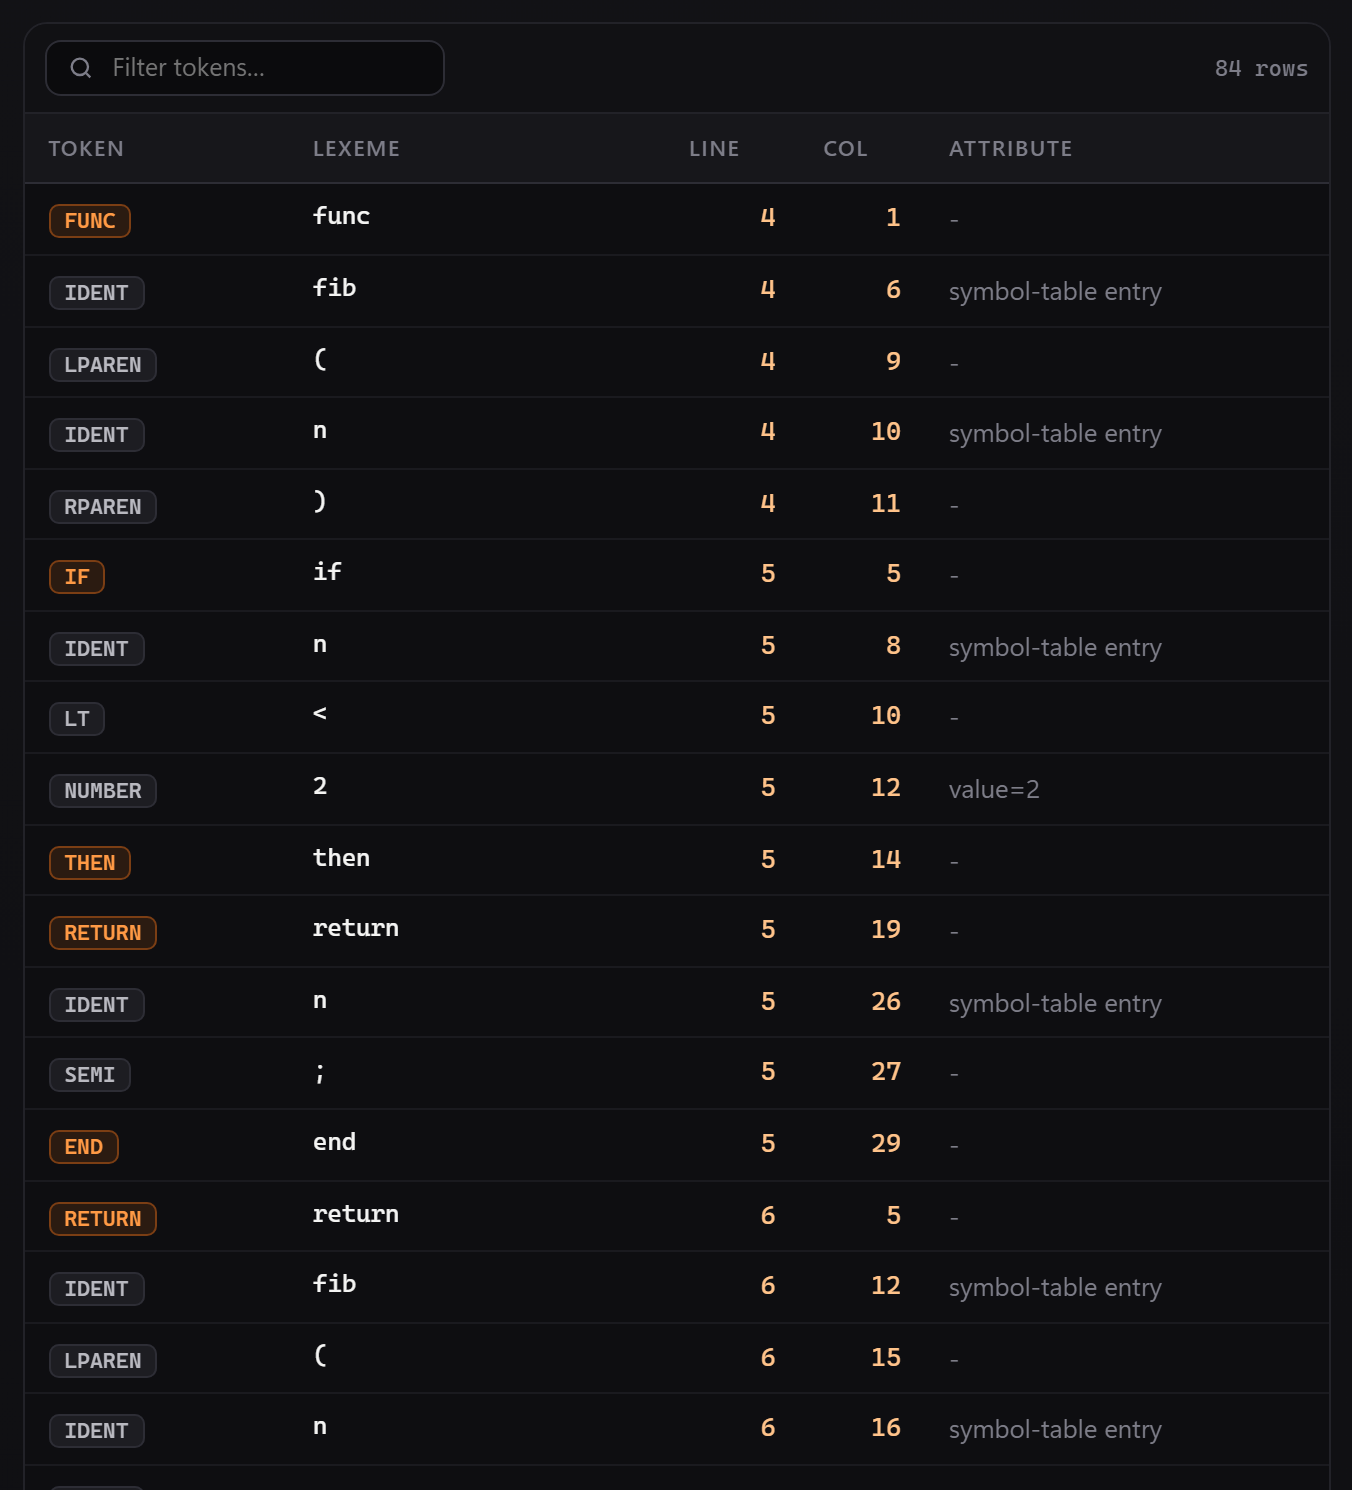
\includegraphics[width=0.92\columnwidth]{figures/token-table.png}
\caption{The token table of the Fibonacci program, first 18 of 84 tokens: kind, lexeme, line, column and the attribute the scanner attaches---the value of a number, the text of a string, or a pointer to the symbol table for an identifier.}
\label{fig:tokentable}
\end{figure}

\subsection{Syntax Analysis}
\label{sec:syntax}
\emph{Grammar analysis.} The grammar module computes FIRST and FOLLOW sets and the LL(1) table and explains every conflict. It then applies left-recursion elimination ($A \to A\alpha \mid \beta$ becomes $A \to \beta A'$, $A' \to \alpha A' \mid \varepsilon$) and left factoring, and re-checks the table. The Nova grammar is written left-recursively to obtain left-associative operators, so it is deliberately not LL(1); Section~\ref{sec:res-front} quantifies this, and Fig.~\ref{fig:ll1} shows the explanations. FIRST and FOLLOW sets for all 20 non-terminals are tabulated (Fig.~\ref{fig:firstfollow}), and the left-recursion elimination reports, non-terminal by non-terminal, how many left-recursive productions it rewrote (Fig.~\ref{fig:leftrec}): eleven non-terminals are affected, eighteen productions in all, with \code{rel} contributing four and \code{term} three.

\emph{LR tables.} From the same grammar, the LR module builds the canonical collection of LR(0) items and derives the SLR(1) table from it, using FOLLOW sets for reductions. It builds the canonical collection of LR(1) items $[A \to \alpha \cdot \beta,\ a]$ for the CLR(1) table, and builds the LALR(1) table by merging LR(1) states that share an LR(0) core:
\begin{equation}
I^{\mathrm{LALR}}_{K} = \bigcup \{\, I \in \mathcal{C}_{\mathrm{LR}(1)} \;:\; \mathrm{core}(I) = K \,\}.
\label{eq:lalr}
\end{equation}
Conflicts are not merely detected but explained: the module names the colliding actions, the look-ahead and the responsible productions. A deliberately ambiguous five-production expression grammar demonstrates genuine shift/reduce conflicts (Fig.~\ref{fig:ambiguous}).

\emph{The automaton, browsable.} The studio exposes the LALR(1) automaton directly (Fig.~\ref{fig:automaton}). For any of the 116 states it lists the items, with kernel items in bold and the merged look-ahead sets in braces, and beside them the ACTION entries (shift, with the target state linked; reduce, with the production; accept) and the GOTO entries. The ACTION/GOTO table itself can be paged through eighteen states at a time (Fig.~\ref{fig:lrtable}); only the columns that are used in the window are shown, so the sparsity of the table is visible. State 26 (Fig.~\ref{fig:lrstate26}) shows the classic decision that LR parsing makes with one token of look-ahead. After an identifier inside an expression, a left parenthesis means a call, so it is shifted; any of the 19 other terminals that may follow an expression means the identifier was a variable, so production 52 of the augmented grammar, \code{factor $\to$ IDENT}, is reduced. No other state needs to know which of the two the identifier was. Because the automaton depends only on the language, it is computed once when the server starts and served to the browser as a 160\,KB JSON document that is fetched a single time.

\emph{Two parsers, one language.} The abstract syntax tree (AST) used by later phases is built by a hand-written recursive-descent parser with one token of look-ahead, a precedence-climbing expression chain and panic-mode recovery. On an error the parser skips to the next token that can start a statement, or to \code{end}, \code{else}, \code{when} or \code{otherwise}, so that one missing semicolon does not cause a cascade of errors. Independently, a table-driven LALR(1) driver parses the same token stream and records the state stack, the symbol stack, the remaining input and the action at every step. Agreement between the two parsers is a self-test. The recursive-descent parser's own call trace, with the look-ahead token that chose each procedure, is shown beside it (Fig.~\ref{fig:rdtrace}); for the Fibonacci program it makes 15 procedure calls where the LALR(1) driver takes 297 actions, because one call consumes a whole statement while the driver shifts and reduces symbol by symbol. Fig.~\ref{fig:syntax} shows the three tables measured on the grammar and Fig.~\ref{fig:lrtrace} the complete trace.

\emph{The parse player.} The trace is also replayed by a player (Fig.~\ref{fig:player}). At any step it shows the state stack with its top highlighted, the symbol stack with the handle about to be reduced marked, the remaining input as a tape with the look-ahead first, the action taken, and the kernel items of the current state, so a learner can see \emph{why} the table says shift or reduce. The player steps forward and back, scrubs, and autoplays at 420\,ms per action; the space bar and the arrow keys drive it when it has focus. At the last step (Fig.~\ref{fig:playeraccept}) the stacks have been reduced to state 1 with the single symbol \code{program}, the input is exhausted, and the kernel item \code{program$'$ $\to$ program $\bullet$} licenses \code{accept}.

\begin{figure}[!t]
\centering
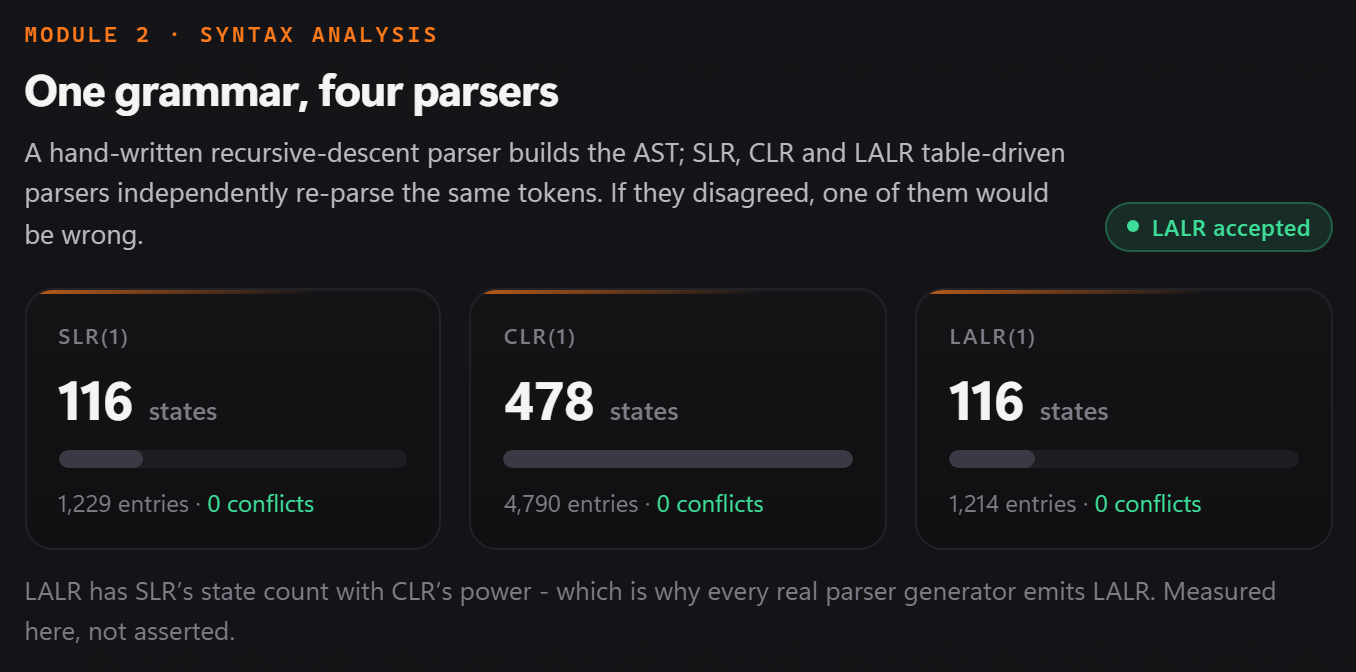
\includegraphics[width=\columnwidth]{figures/view-syntax.png}
\caption{Syntax view: the SLR(1), CLR(1) and LALR(1) tables for the 58-production Nova grammar, with state counts, table entries and conflicts measured on the real grammar. The LALR(1) driver accepted the program.}
\label{fig:syntax}
\end{figure}

\begin{figure}[!t]
\centering
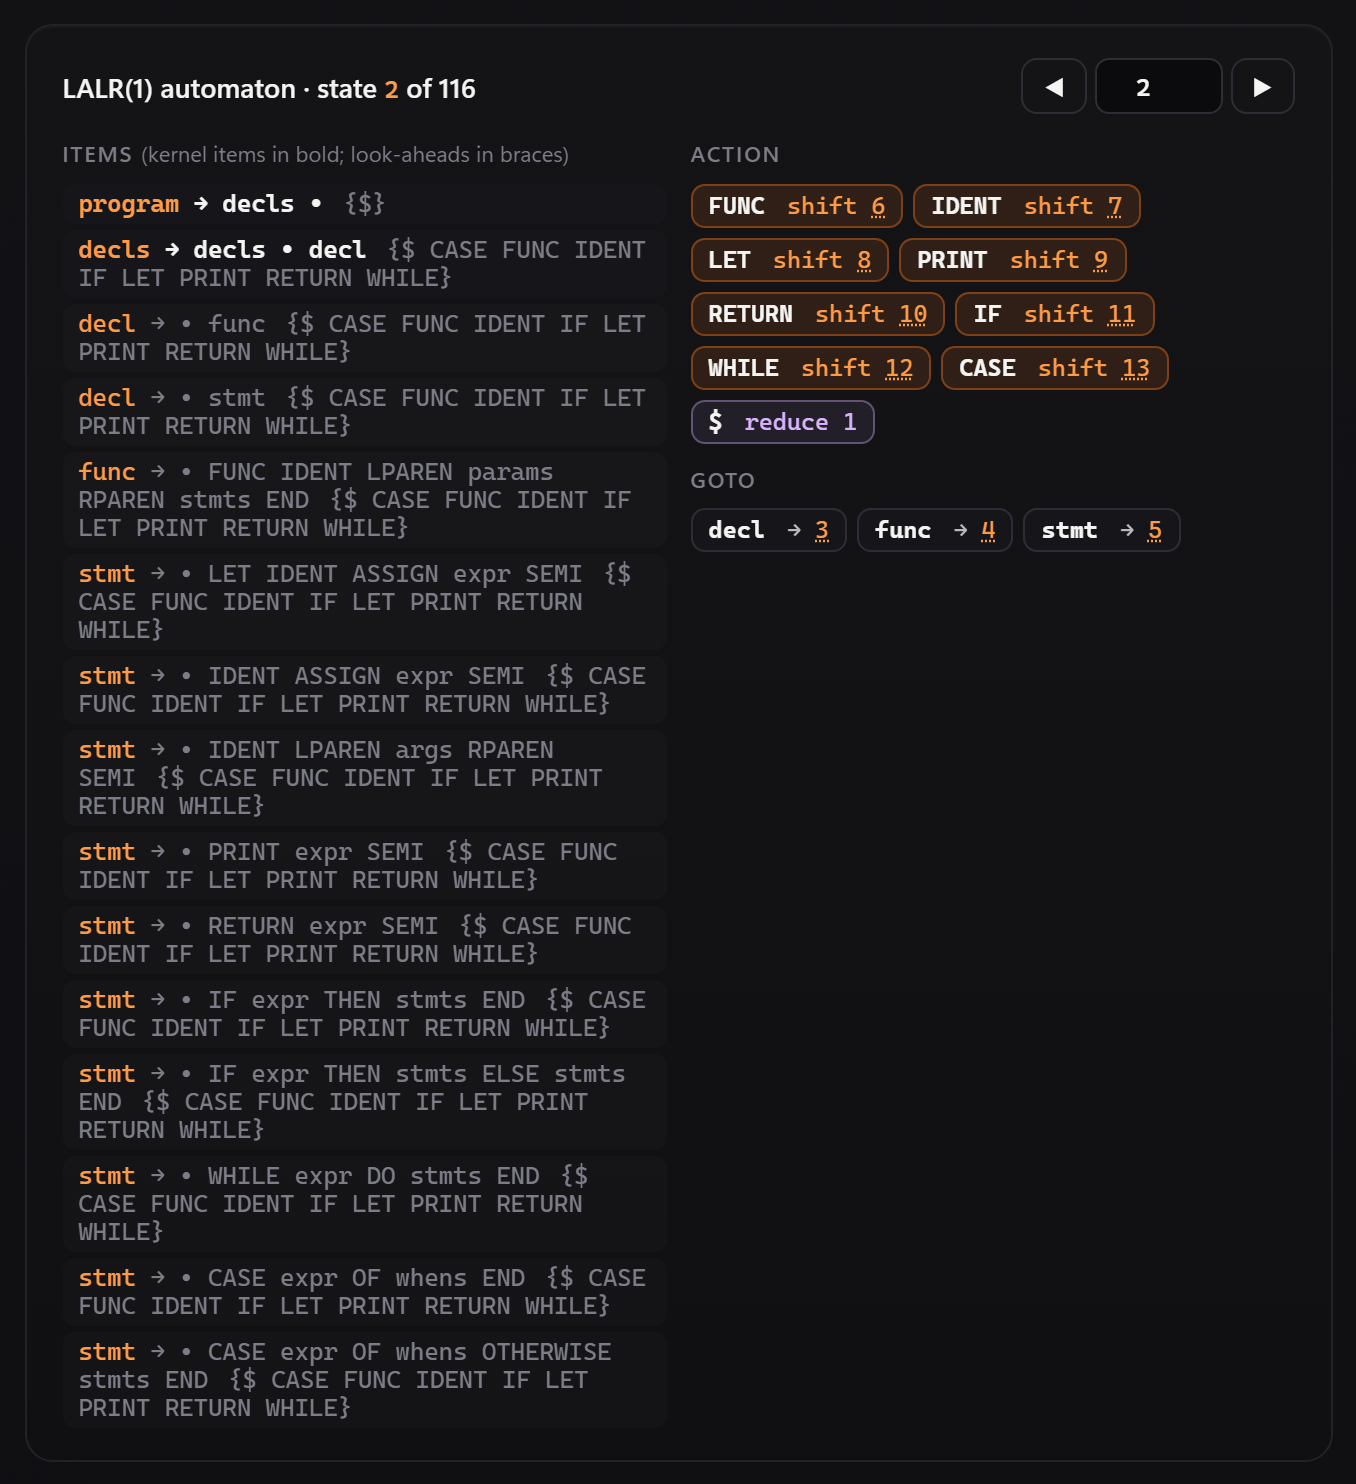
\includegraphics[width=0.95\columnwidth]{figures/lr-automaton.png}
\caption{The automaton browser on state 2 of the LALR(1) automaton. Left: the kernel item \code{program $\to$ decls $\bullet$} and the closure items for every statement form, each with its merged look-ahead set. Right: the ACTION row (shift on each statement-starting terminal, reduce production 1 on end of input) and the GOTO row. Shift targets and GOTO targets are links to the next state.}
\label{fig:automaton}
\end{figure}

\begin{figure}[!t]
\centering
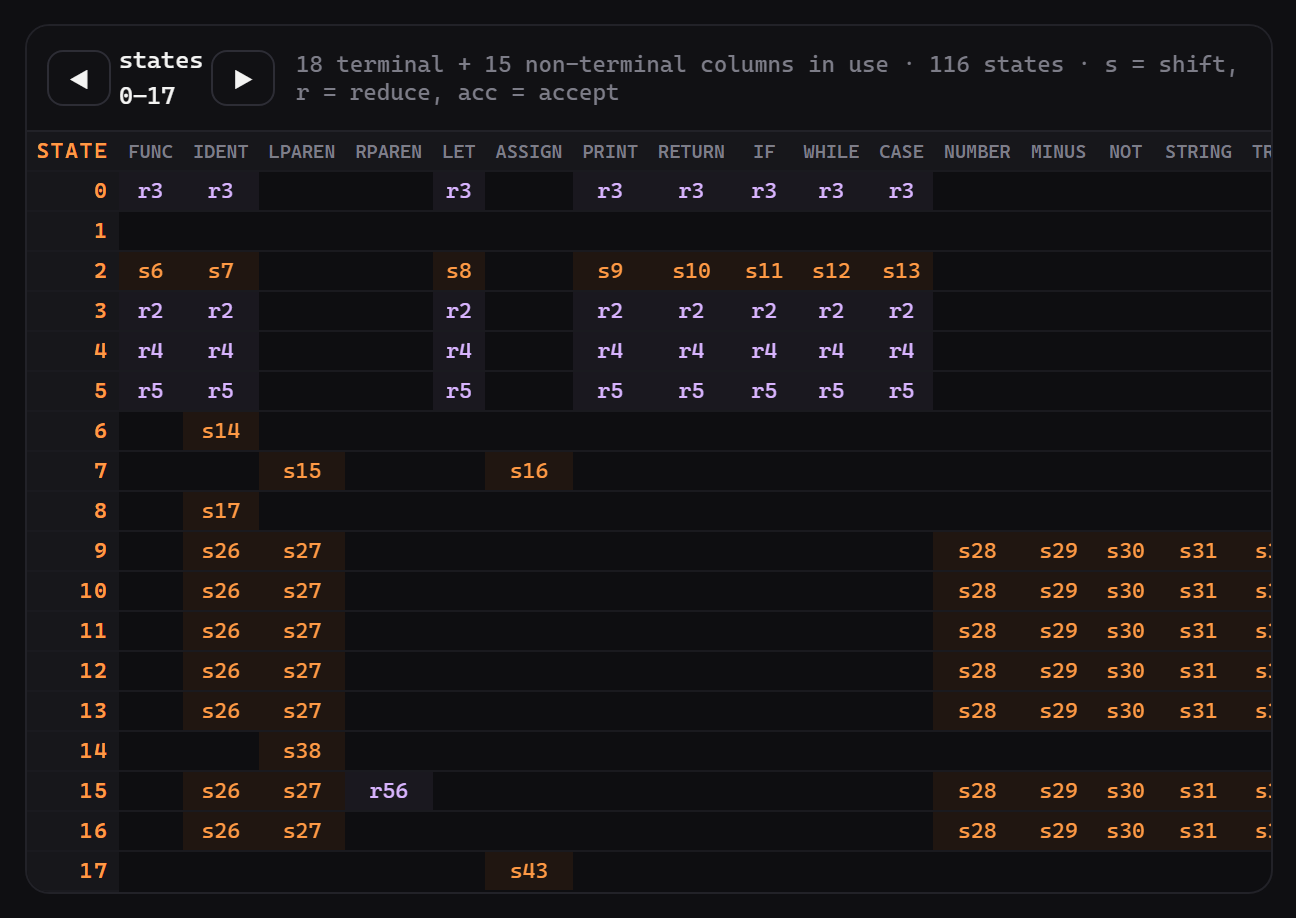
\includegraphics[width=\columnwidth]{figures/lr-table.png}
\caption{The ACTION/GOTO table, states 0--17 of 116. Shift entries are orange, reduce entries violet, accept green; only the 18 terminal and 15 non-terminal columns used in this window are drawn. States 9--13 and 15--16 share one row pattern because they all expect an expression.}
\label{fig:lrtable}
\end{figure}

\begin{figure}[!t]
\centering
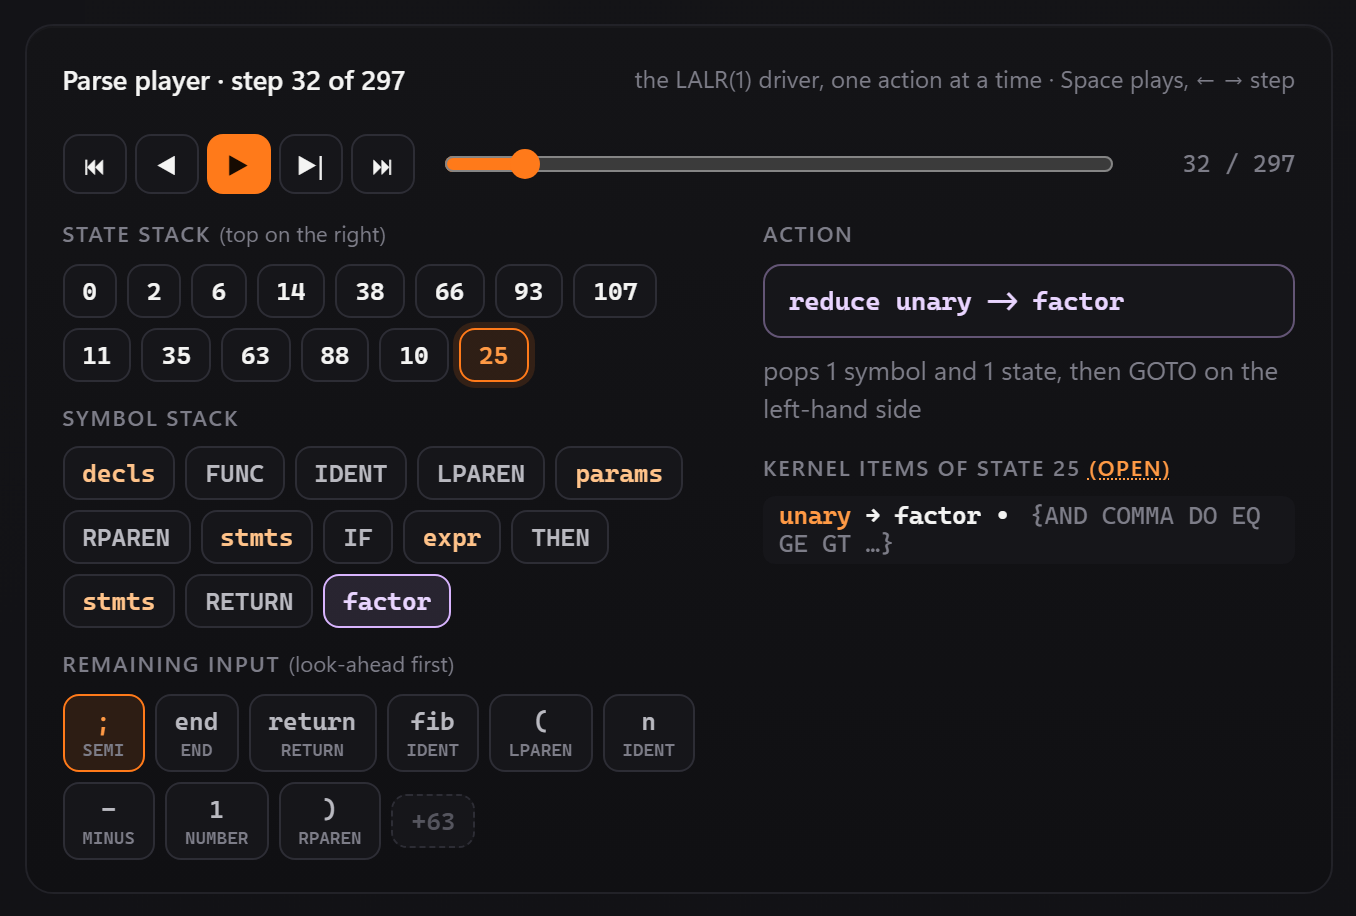
\includegraphics[width=\columnwidth]{figures/parse-player.png}
\caption{The parse player at step 32 of the 297-step LALR(1) parse of the Fibonacci program. The state stack has state 25 on top; the symbol stack ends in the handle \code{factor} (marked), which the action \code{reduce unary $\to$ factor} pops before a GOTO on \code{unary}; the tape shows the look-ahead \code{;} and the next tokens; the kernel item of state 25 explains the reduction.}
\label{fig:player}
\end{figure}

\begin{figure*}[!t]
\centering
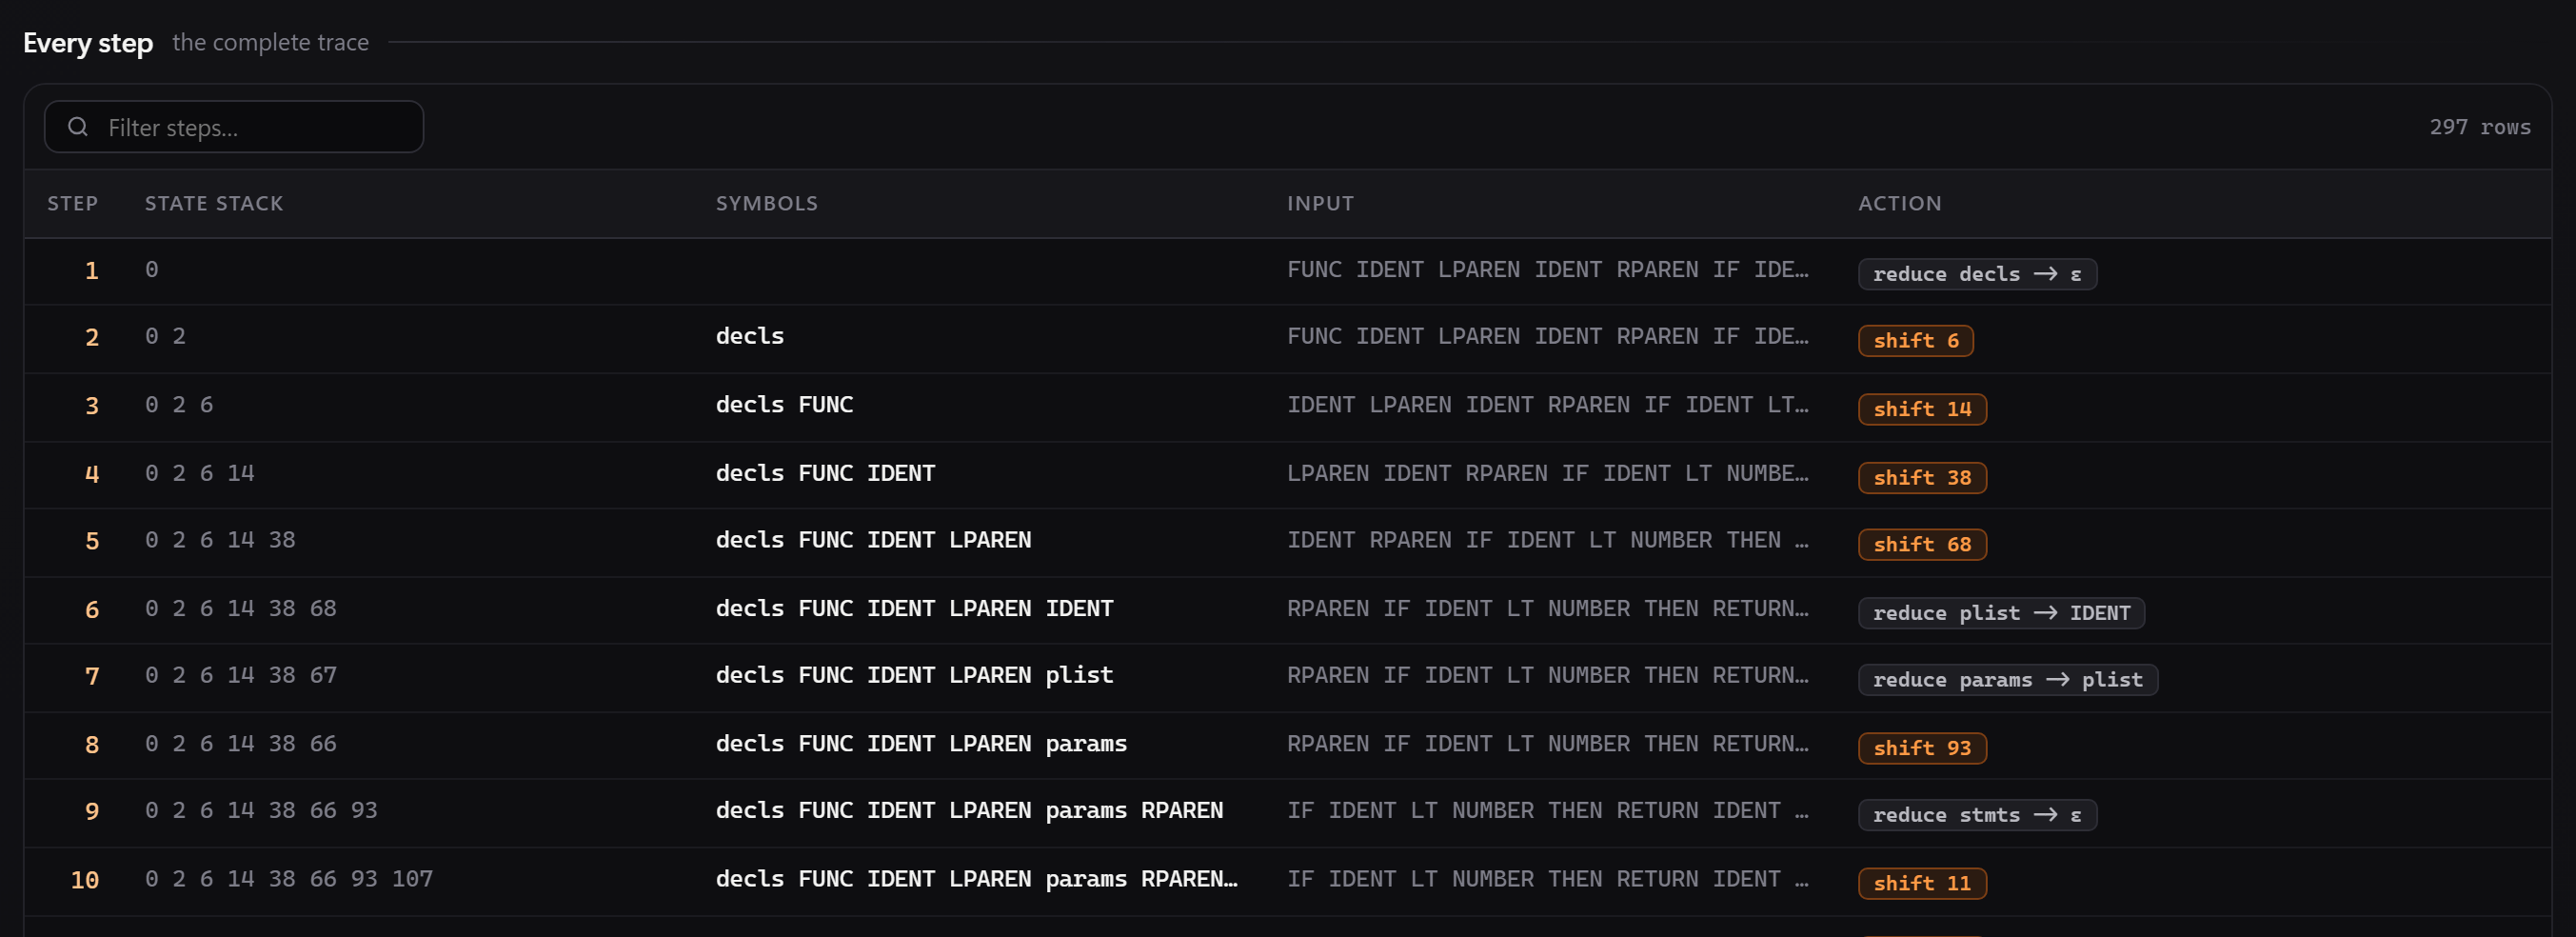
\includegraphics[width=0.92\textwidth]{figures/view-lrtrace.png}
\caption{The first ten of 297 steps of the LALR(1) parse of the Fibonacci program, as the studio tabulates them: state stack, symbol stack, remaining input and the shift or reduce action taken. The filter box searches all steps.}
\label{fig:lrtrace}
\end{figure*}

\begin{figure}[!t]
\centering
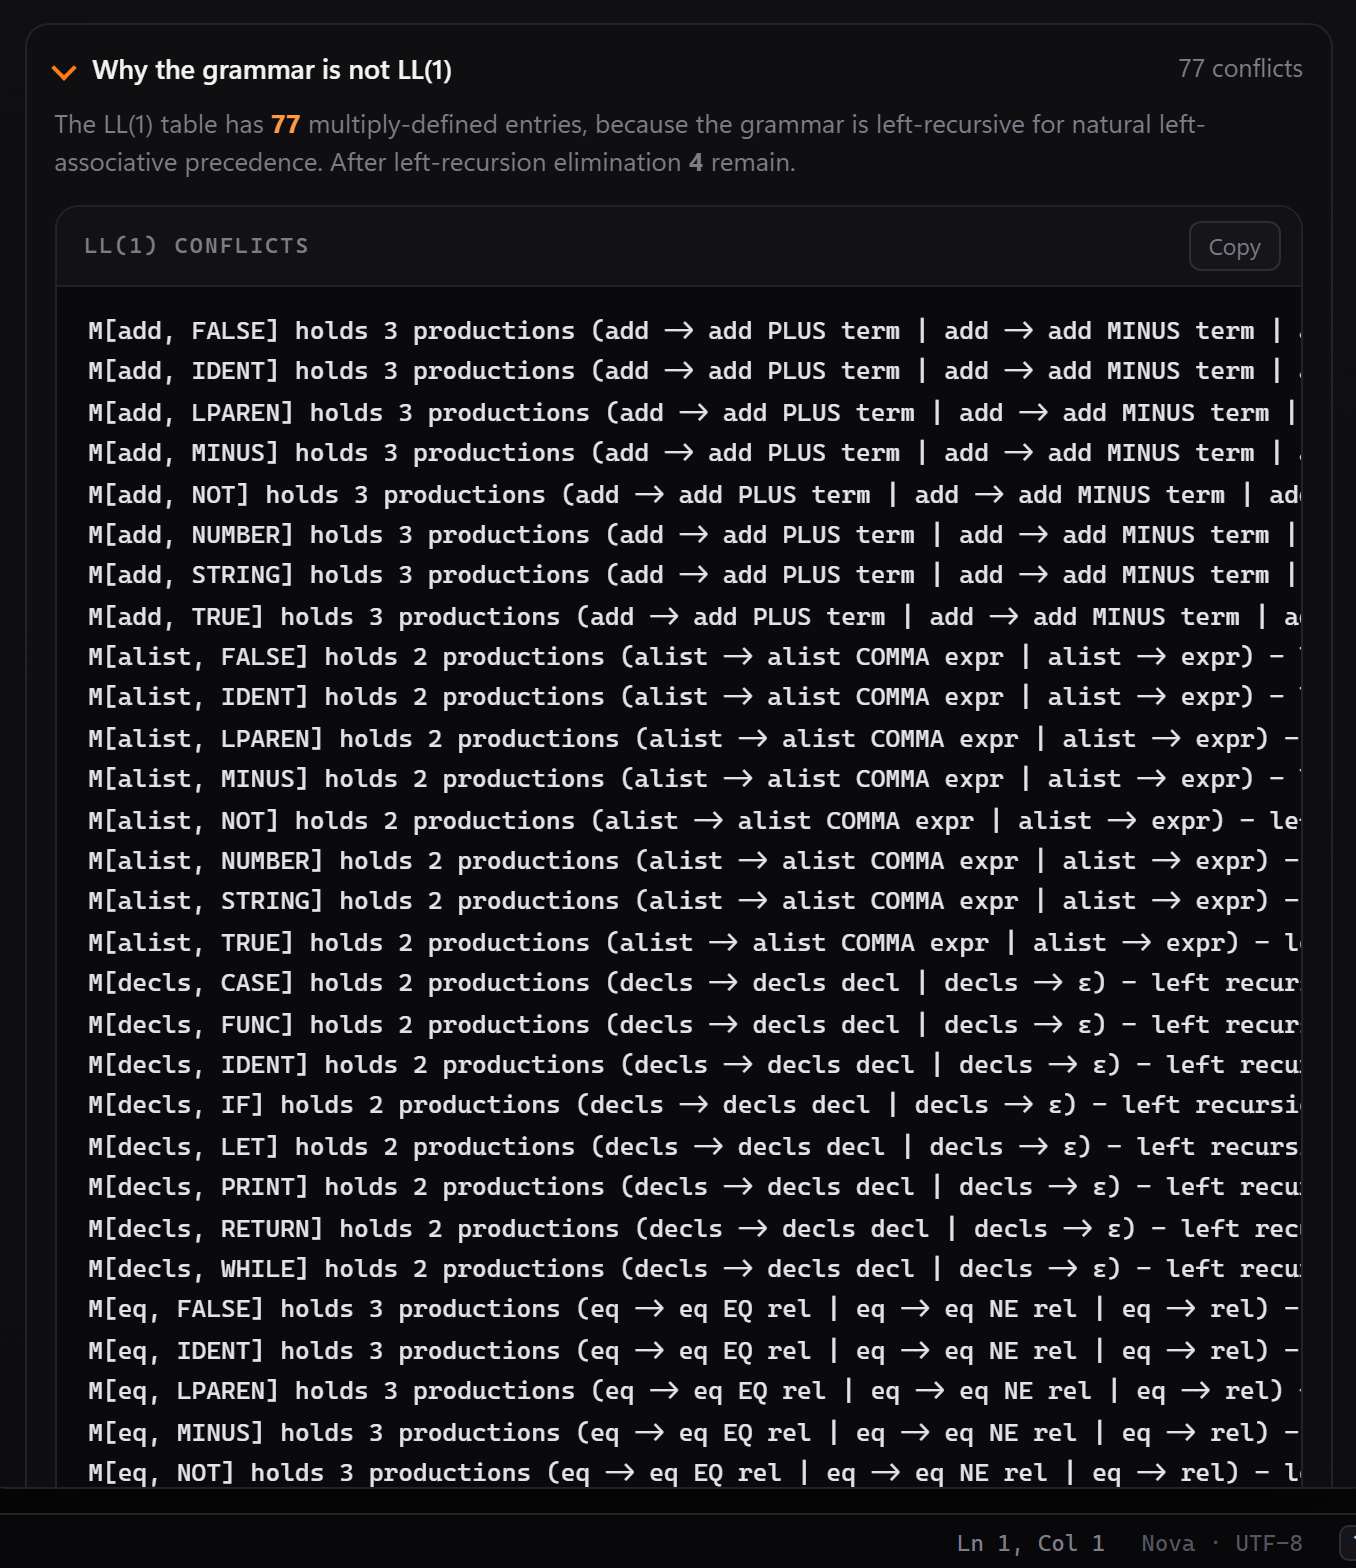
\includegraphics[width=\columnwidth]{figures/ll1-conflicts.png}
\caption{Why the grammar is not LL(1): the first of 77 multiply defined table entries, each naming the productions that collide and the reason---left recursion---and the count of 4 that remain after left-recursion elimination.}
\label{fig:ll1}
\end{figure}

\begin{figure}[!t]
\centering
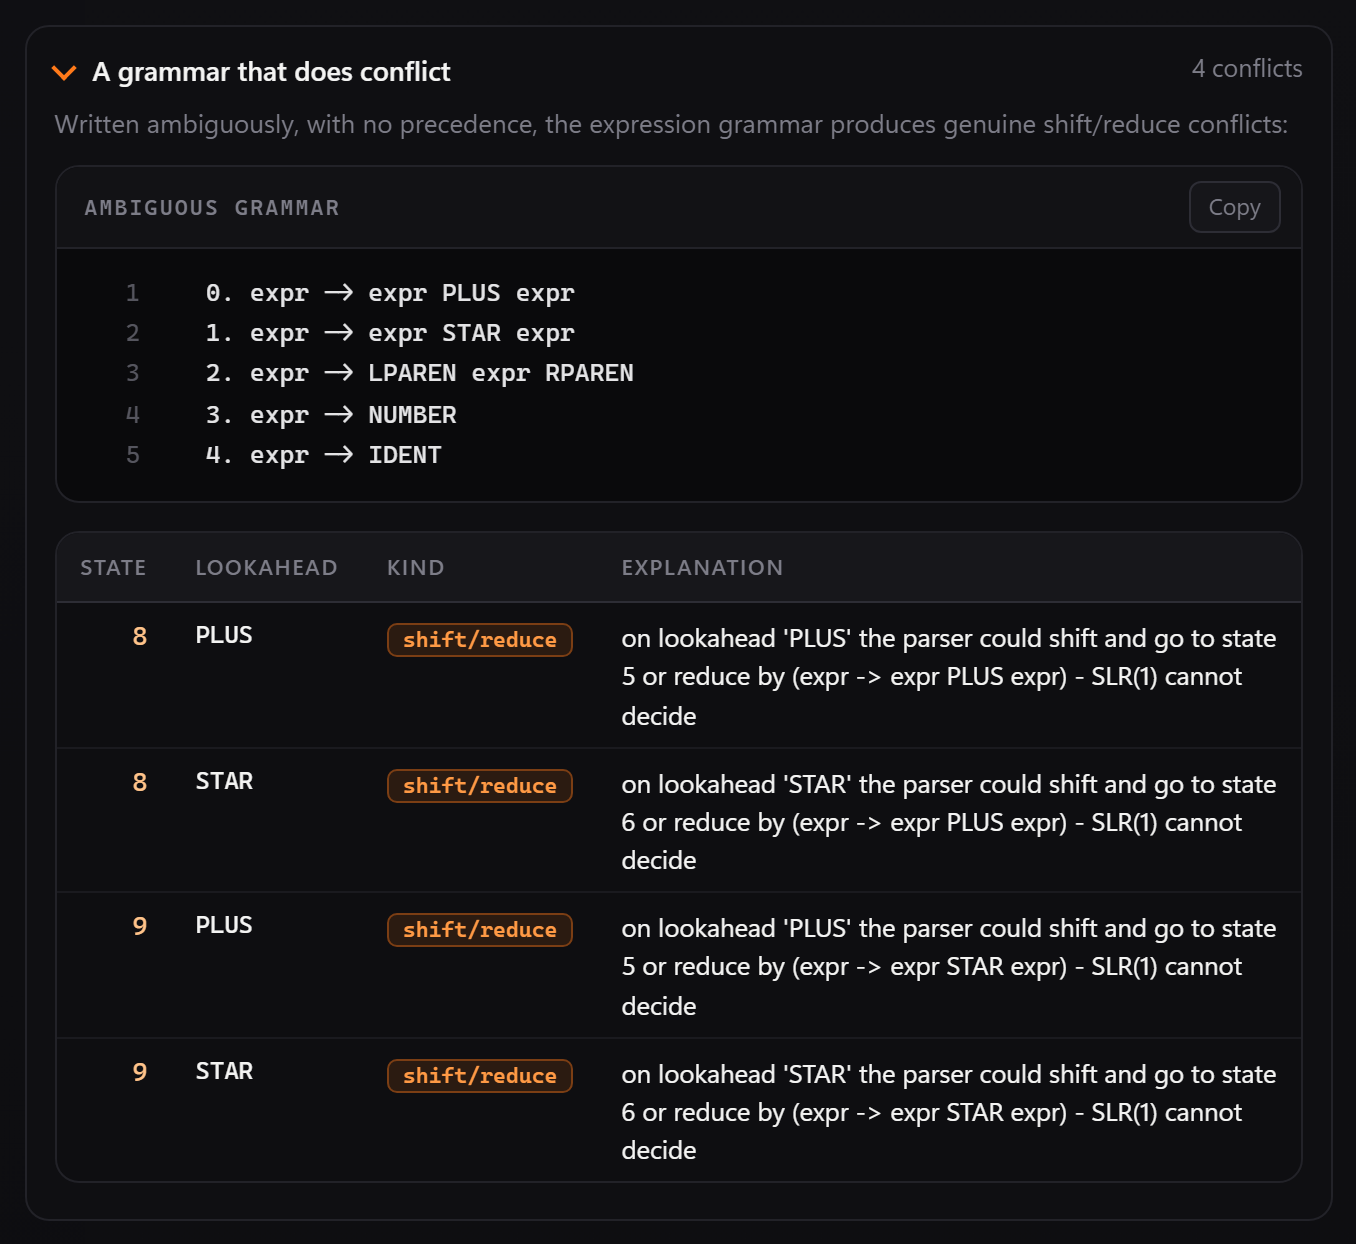
\includegraphics[width=\columnwidth]{figures/ambiguous-grammar.png}
\caption{A grammar that does conflict. The five-production expression grammar without precedence produces four shift/reduce conflicts under SLR(1) construction, two in each of states 8 and 9 on \code{+} and \code{*}; the explanation names the items that collide.}
\label{fig:ambiguous}
\end{figure}

\begin{figure}[!t]
\centering
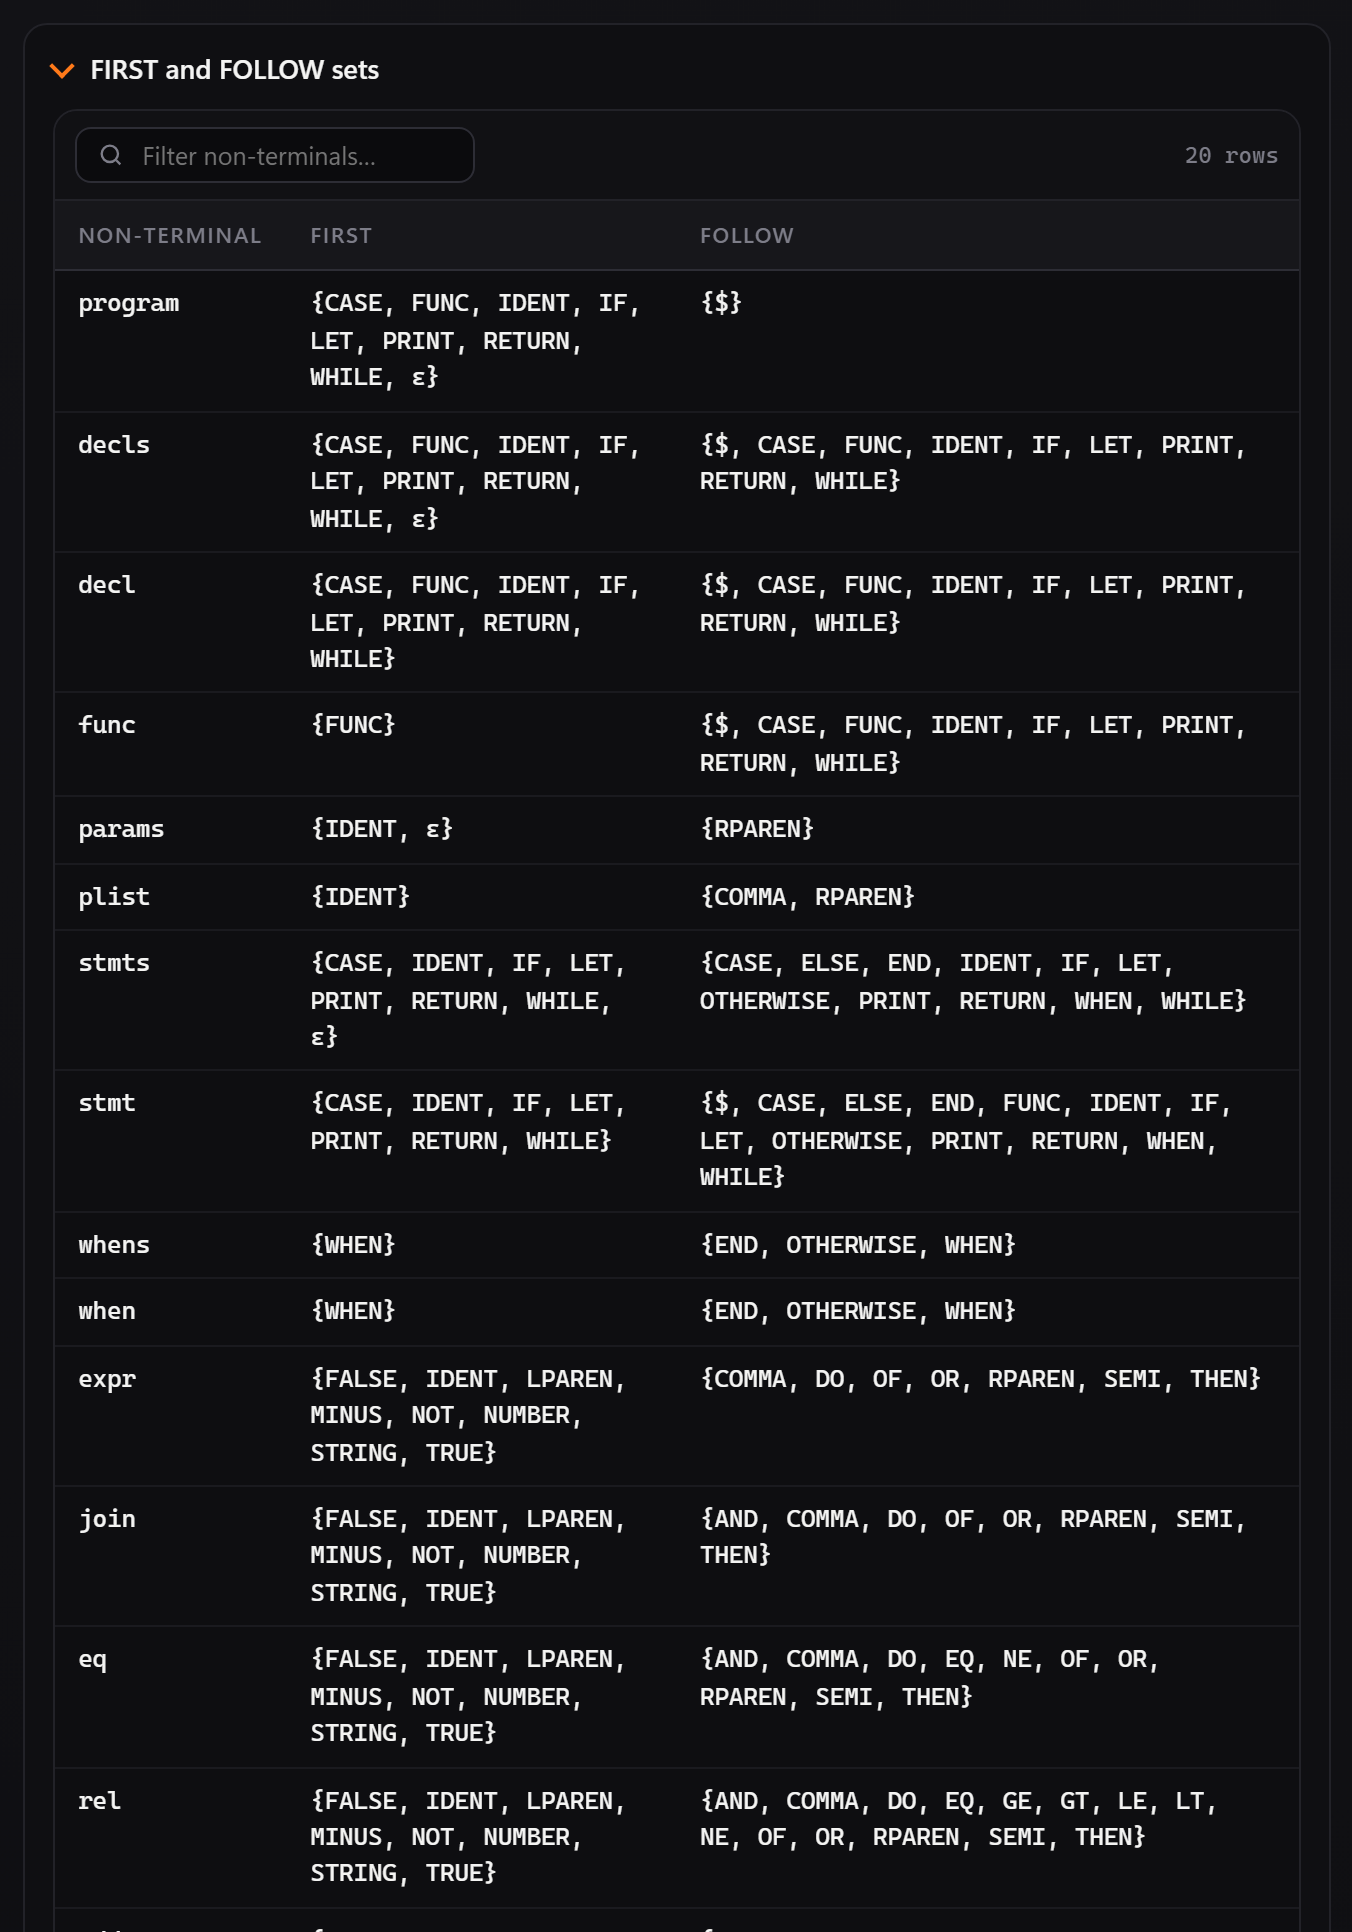
\includegraphics[width=0.92\columnwidth]{figures/first-follow.png}
\caption{FIRST and FOLLOW sets of the first 14 of the 20 non-terminals. \code{decls}, \code{params}, \code{stmts} and \code{args} can be empty, so their FIRST sets include $\varepsilon$; the FOLLOW set of \code{stmts} contains exactly the tokens that may end a block (\code{END}, \code{ELSE}, \code{WHEN}, \code{OTHERWISE}) together with every statement-starting token.}
\label{fig:firstfollow}
\end{figure}

\begin{figure}[!t]
\centering
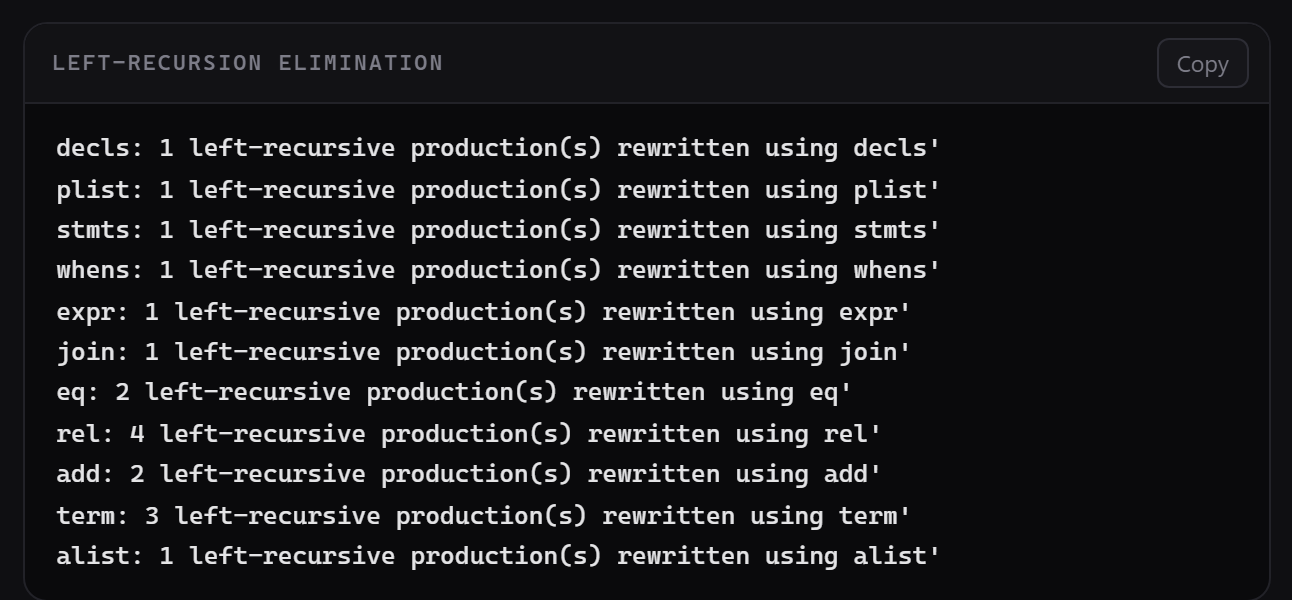
\includegraphics[width=\columnwidth]{figures/left-recursion.png}
\caption{The left-recursion elimination log: eleven non-terminals each receive a primed companion, \code{A$'$}, into which their left-recursive productions are rewritten. The operator chain from \code{expr} to \code{term} accounts for thirteen of the eighteen rewritten productions.}
\label{fig:leftrec}
\end{figure}

\begin{figure}[!t]
\centering
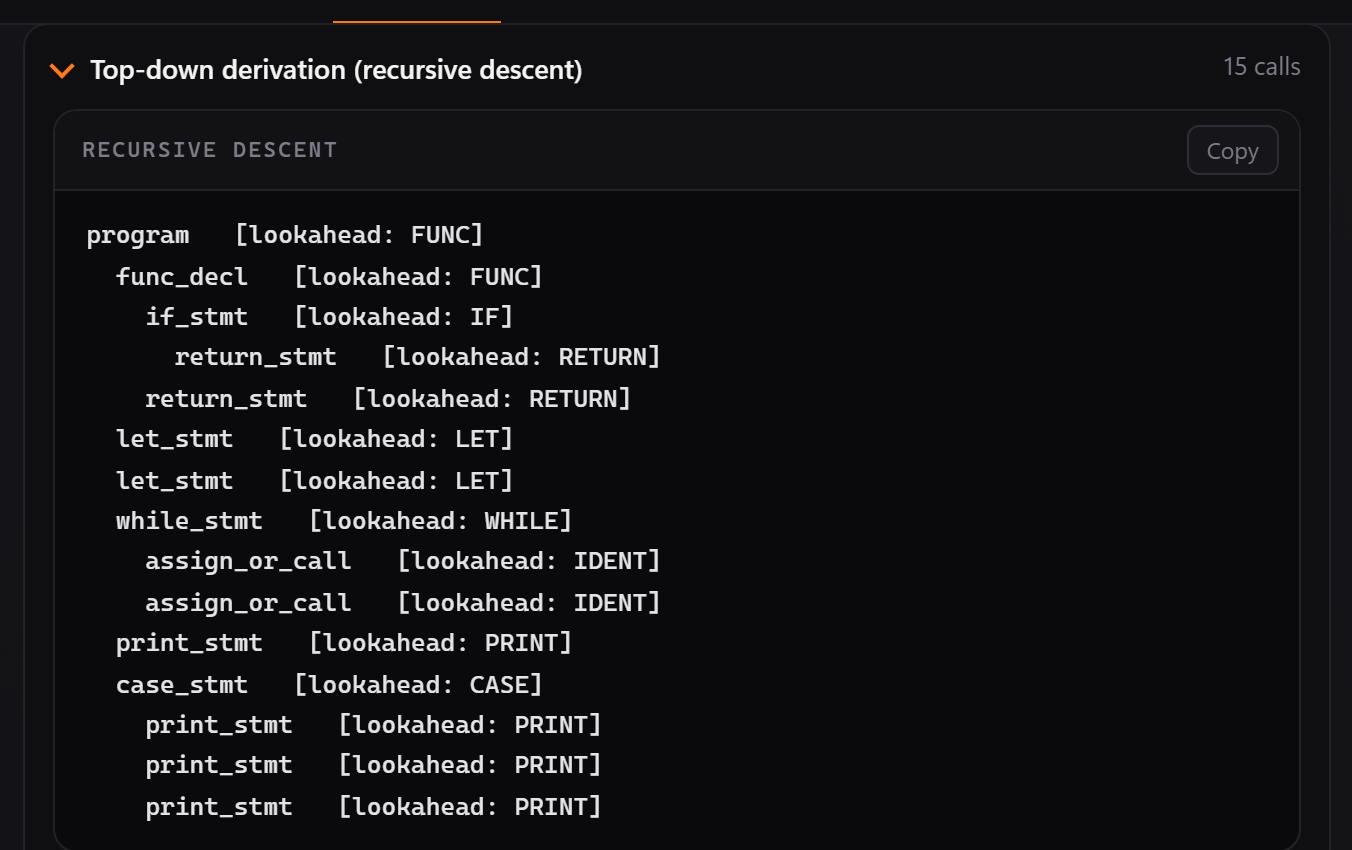
\includegraphics[width=\columnwidth]{figures/rd-trace.png}
\caption{The top-down derivation of the Fibonacci program by the recursive-descent parser: one line per procedure call, indented by nesting depth, with the look-ahead token that selected the procedure. The \code{case} statement calls \code{print\_stmt} once for each arm.}
\label{fig:rdtrace}
\end{figure}

\begin{figure}[!t]
\centering
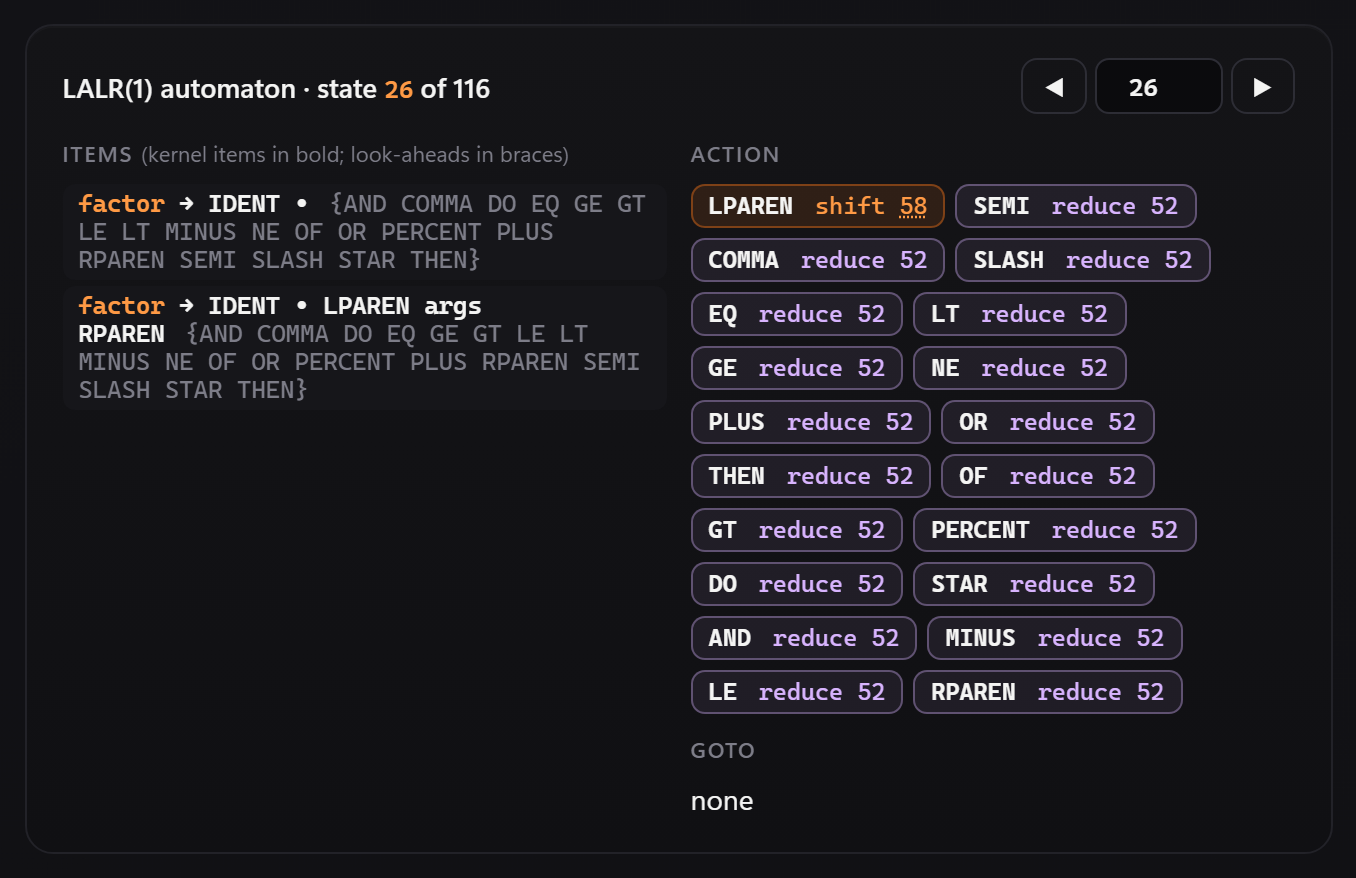
\includegraphics[width=\columnwidth]{figures/lr-state-26.png}
\caption{State 26 of the LALR(1) automaton, reached after an \code{IDENT} inside an expression. The two kernel items share the prefix \code{IDENT}; the look-ahead decides between them: \code{LPAREN} is shifted (a call), and the 19 terminals that can follow an expression reduce \code{factor $\to$ IDENT} (a variable).}
\label{fig:lrstate26}
\end{figure}

\begin{figure}[!t]
\centering
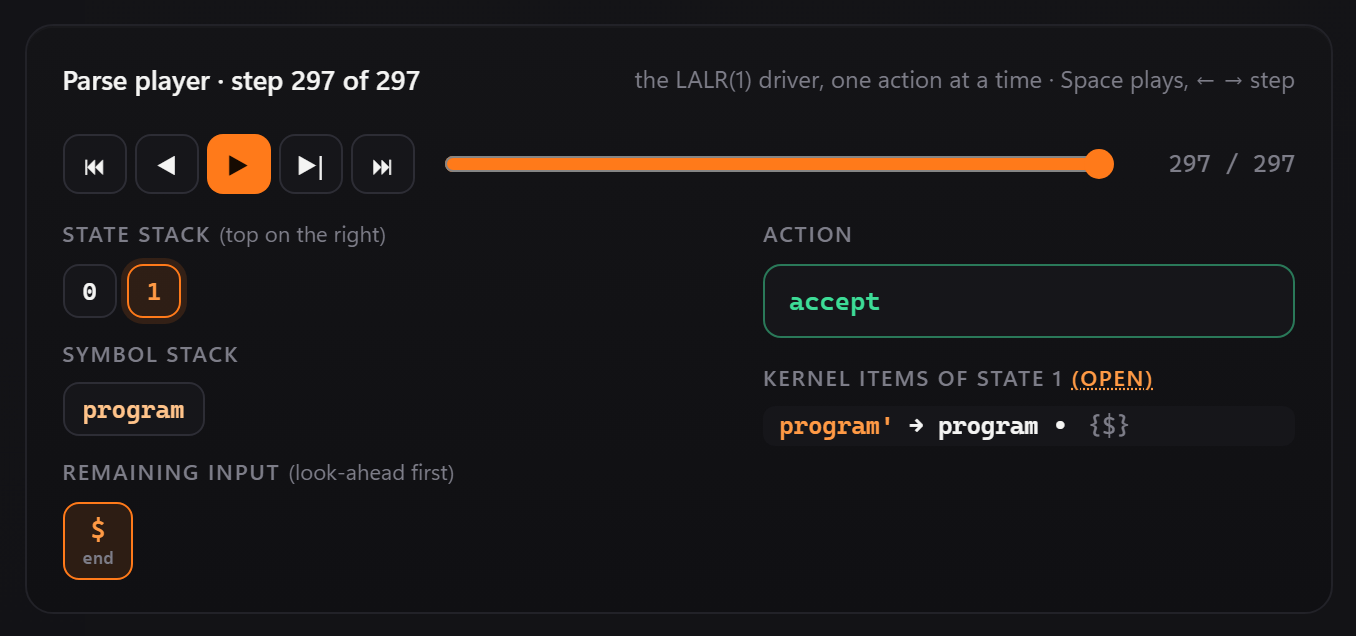
\includegraphics[width=\columnwidth]{figures/parse-player-accept.png}
\caption{The parse player at its last step, 297: the state stack is \code{0 1}, the symbol stack holds only \code{program}, the remaining input is the end marker, and the kernel item of state 1 explains the \code{accept} action.}
\label{fig:playeraccept}
\end{figure}

\subsection{Semantic Analysis}
Semantic analysis is a single L-attributed pass over the AST, preceded by a pass that collects function signatures so that calls may precede declarations. \emph{Inherited} attributes flow downwards: the current scope, the nesting depth, the enclosing function and the type the context expects. \emph{Synthesised} attributes flow upwards: the type of every expression. Each symbol records its name, kind, type, scope, depth, frame slot, declaring line and whether it is used. The type rules are as follows:
\begin{itemize}
\item arithmetic maps $\mathit{int}\times\mathit{int}\to\mathit{int}$, and \code{+} also maps $\mathit{str}\times\mathit{str}\to\mathit{str}$;
\item relational operators produce $\mathit{bool}$, and \code{and}/\code{or}/\code{not} require $\mathit{bool}$;
\item every condition must be $\mathit{bool}$, and every argument must be $\mathit{int}$.
\end{itemize}
A poisoned $\langle\mathit{error}\rangle$ type suppresses cascades. Unused variables produce warnings rather than errors. Every attribute flow is logged per construct (Fig.~\ref{fig:semantic}), and the annotated tree is drawn (Fig.~\ref{fig:ast}): each node carries the type the checker synthesised for it, and the drawing can be switched between the functions and the statements of the main program. Fig.~\ref{fig:astcase} shows the \code{case} statement of the same program: the selector \code{total} synthesises \code{int}, each arm prints a string literal of type \code{str}, and the arms carry no type of their own because statements do not synthesise one. The layout is a simplified Reingold--Tilford tree layout~\cite{reingold1981}: subtrees are measured bottom-up, placed left to right without overlap, and every parent is centred over its children.

\begin{figure}[!t]
\centering
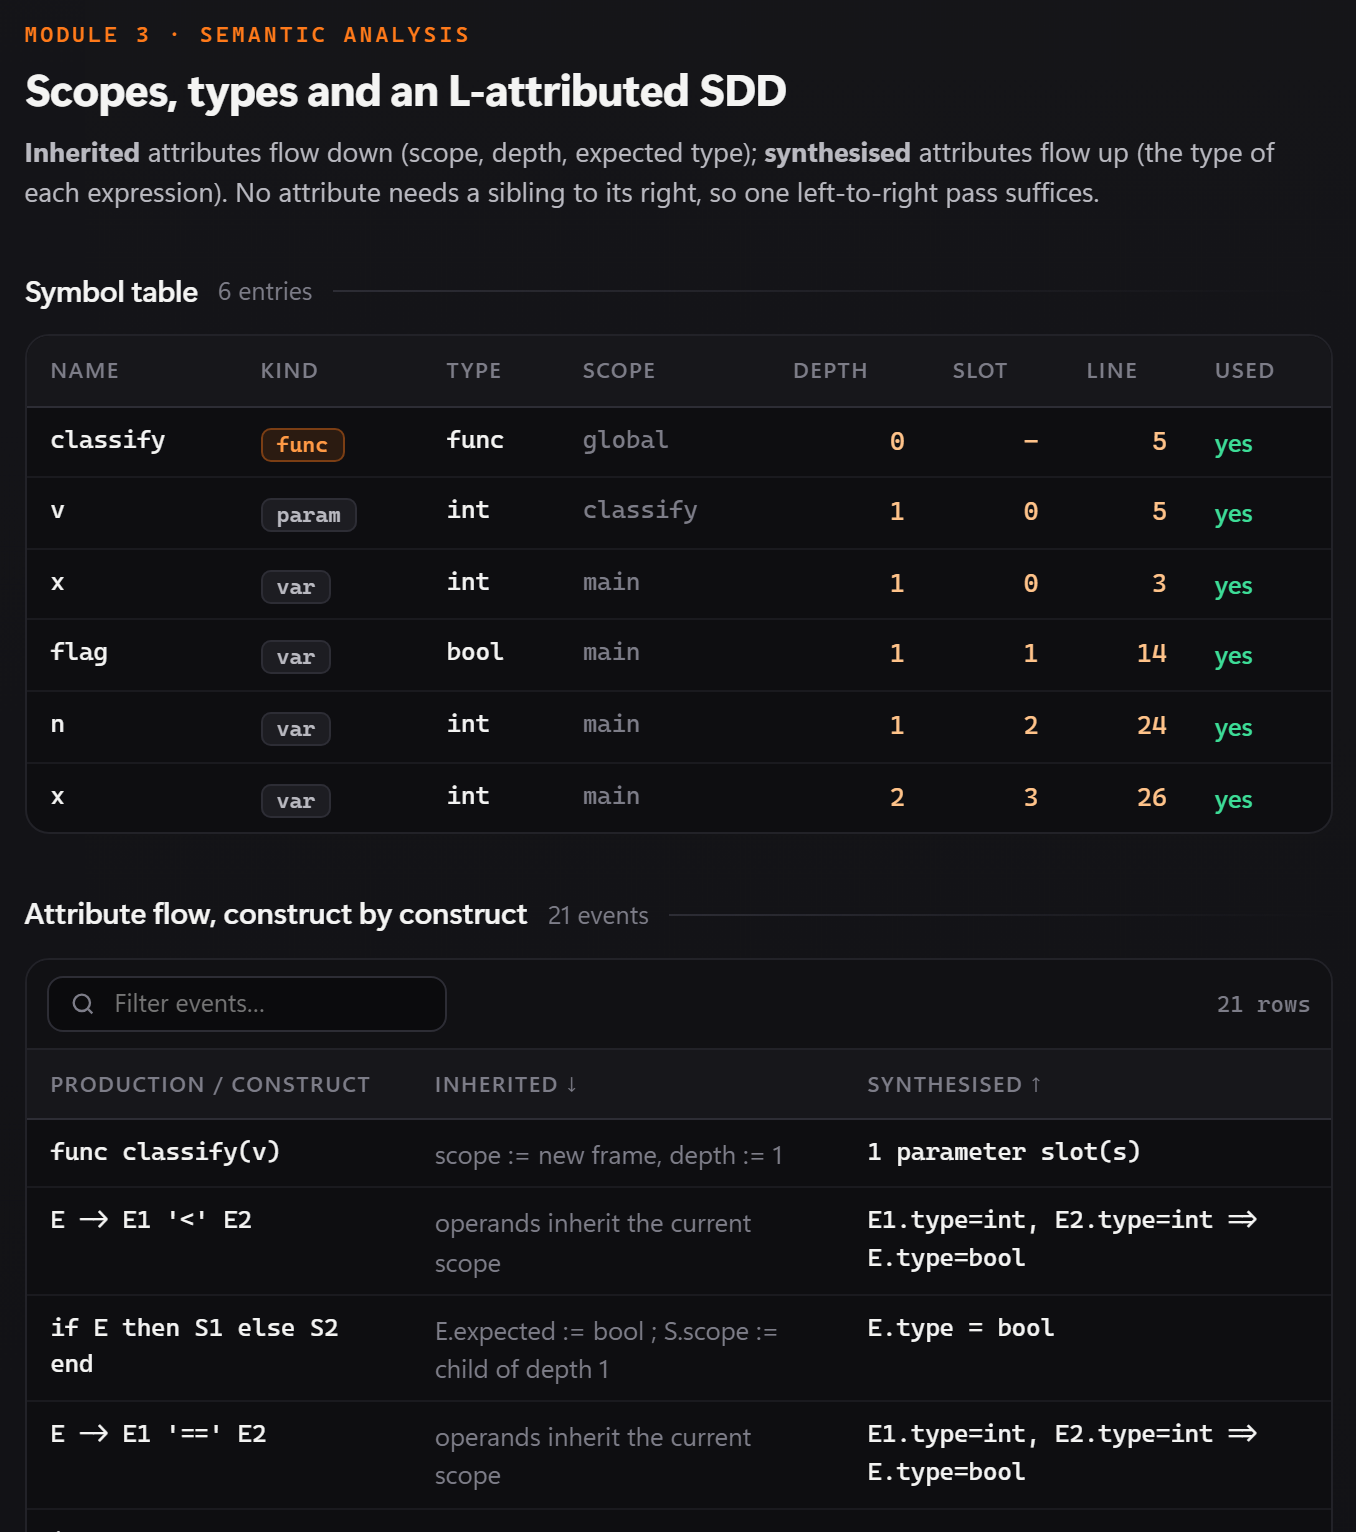
\includegraphics[width=\columnwidth]{figures/view-semantic.png}
\caption{Semantic view of \code{07\_types\_and\_scopes.nova}: the scoped symbol table, in which the inner \code{x} at depth 2 shadows the outer one, and the attribute flow construct by construct, with inherited attributes passed down and synthesised attributes passed up.}
\label{fig:semantic}
\end{figure}

\begin{figure*}[!t]
\centering
\subfloat[The function \code{fib}: the condition synthesises \code{bool}, every arithmetic node and call synthesises \code{int}.]{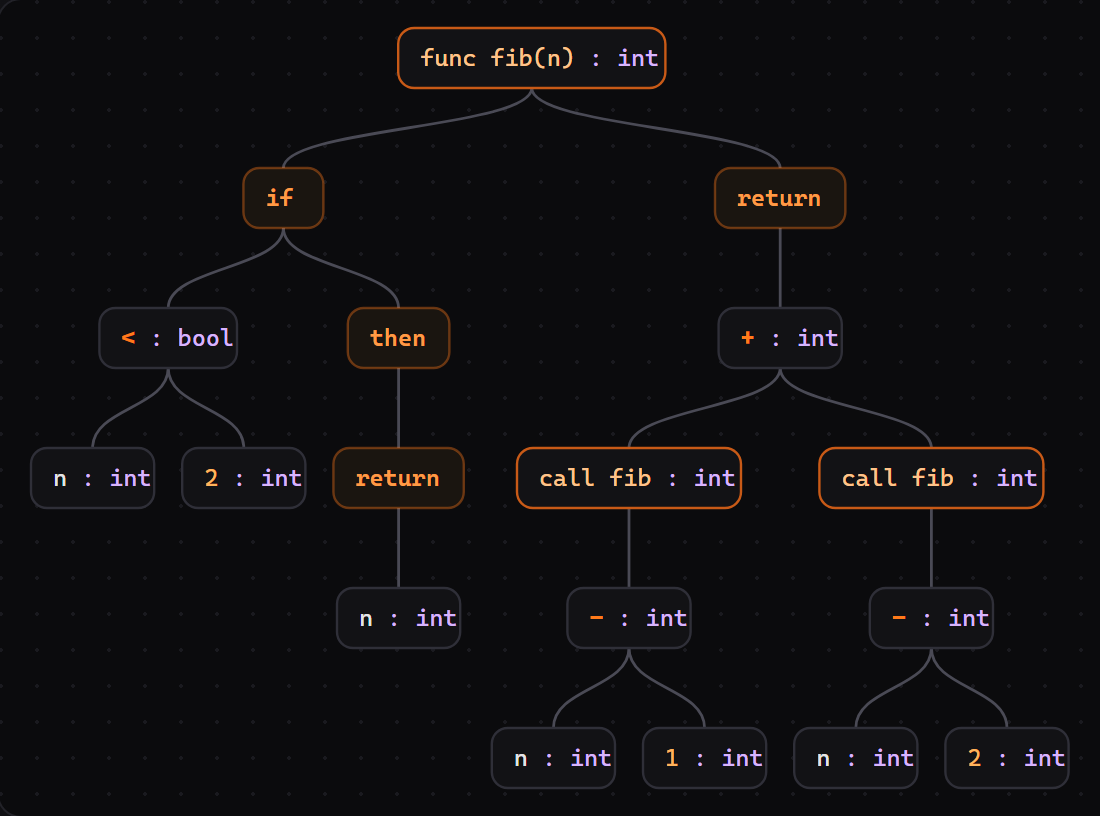
\includegraphics[width=0.49\textwidth]{figures/ast-tree.png}\label{fig:ast-fib}}
\hfil
\subfloat[The \code{while} loop of the main program: its condition and body, with the recursive call inside the accumulation.]{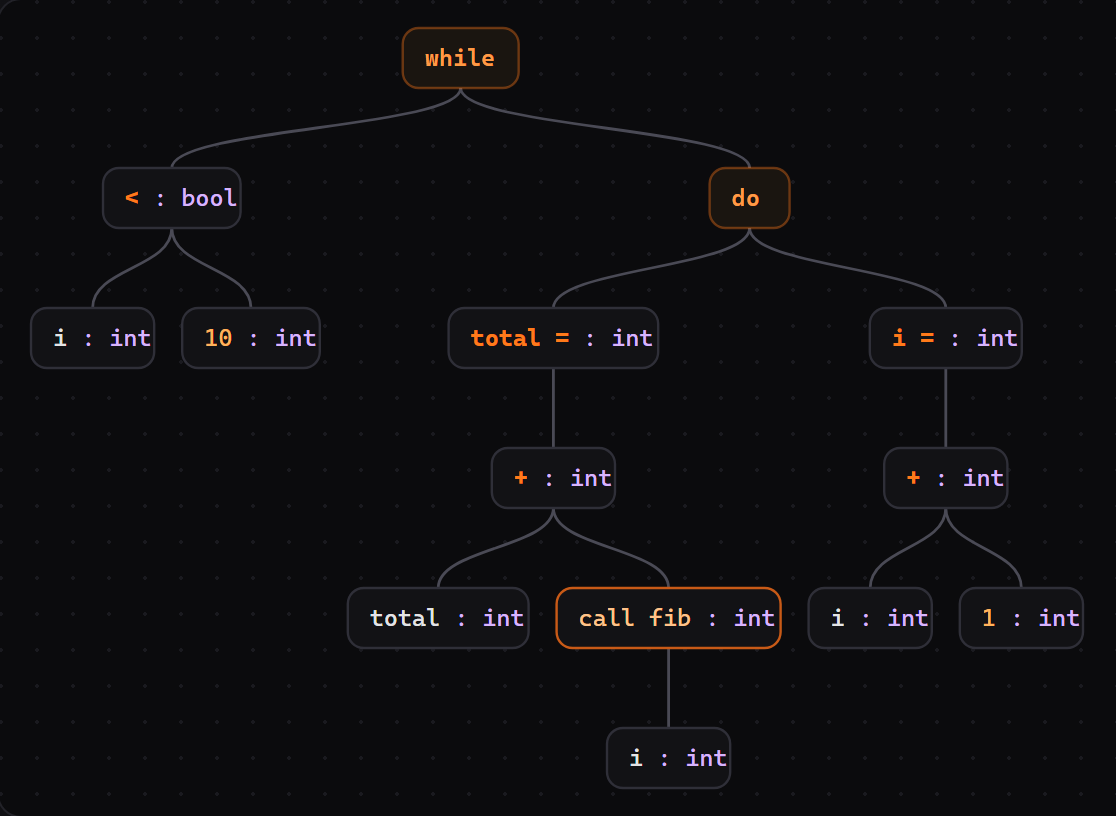
\includegraphics[width=0.49\textwidth]{figures/ast-tree-while.png}\label{fig:ast-while}}
\caption{The annotated syntax tree of the Fibonacci program as the studio draws it. Keywords are orange-bordered, operators orange, literals amber, and the synthesised type attribute follows each node's label in violet.}
\label{fig:ast}
\end{figure*}

\begin{figure}[!t]
\centering
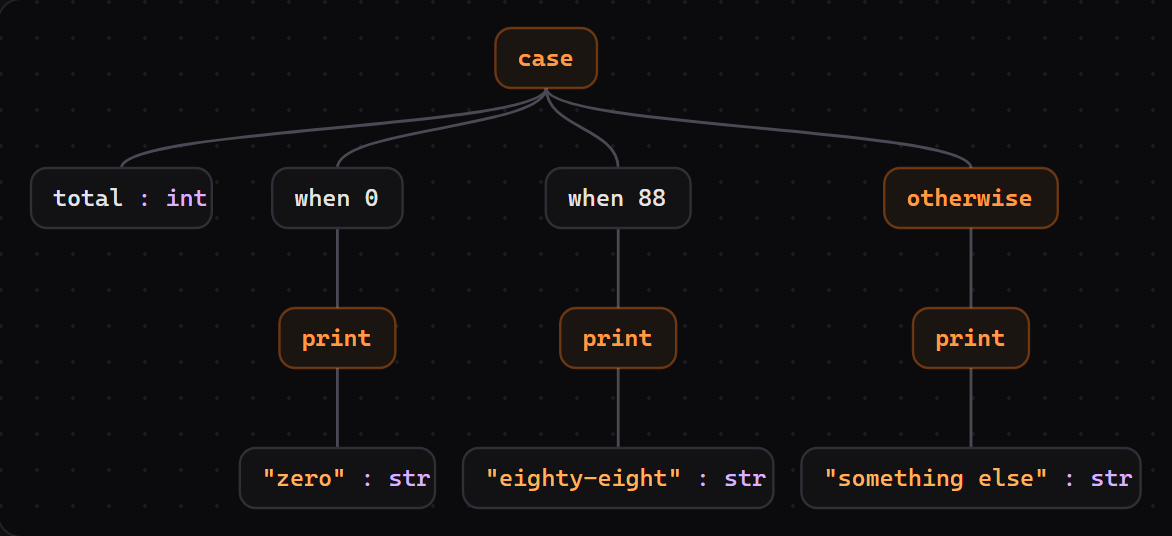
\includegraphics[width=\columnwidth]{figures/ast-case.png}
\caption{The \code{case} statement of the Fibonacci program as an annotated tree: the selector \code{total : int}, the arms \code{when 0} and \code{when 88}, and the \code{otherwise} arm, each holding a \code{print} of a string literal.}
\label{fig:astcase}
\end{figure}

\subsection{Intermediate-Code Generation}
Three-address code is generated as quadruples (\emph{op}, \emph{arg$_1$}, \emph{arg$_2$}, \emph{result}) by a syntax-directed translation scheme. Boolean expressions are compiled as \emph{jumping code} with true and false lists, so \code{a and b} never evaluates \code{b} when \code{a} is false. Jump targets that are unknown when a jump is emitted are left blank and filled in by \code{makelist}, \code{merge} and \code{backpatch}~\cite{aho2006}, and every backpatch is logged (Fig.~\ref{fig:backpatch}). A \code{case} statement is lowered to a genuine jump table (\code{jtab}) with a default target rather than to a chain of comparisons (Fig.~\ref{fig:tac}). Fig.~\ref{fig:tacprimes} shows short-circuit evaluation of \code{isprime(n) == 1 and n > 1} in \code{04\_primes.nova}: the call and the first comparison are emitted as instructions 5--7; only when that comparison holds does control reach the test \code{n > 1} at \code{L2}, and both false exits jump to \code{L4}, past the body. No boolean value is ever materialised: the truth of the condition is represented entirely by where control goes.

\begin{figure}[!t]
\centering
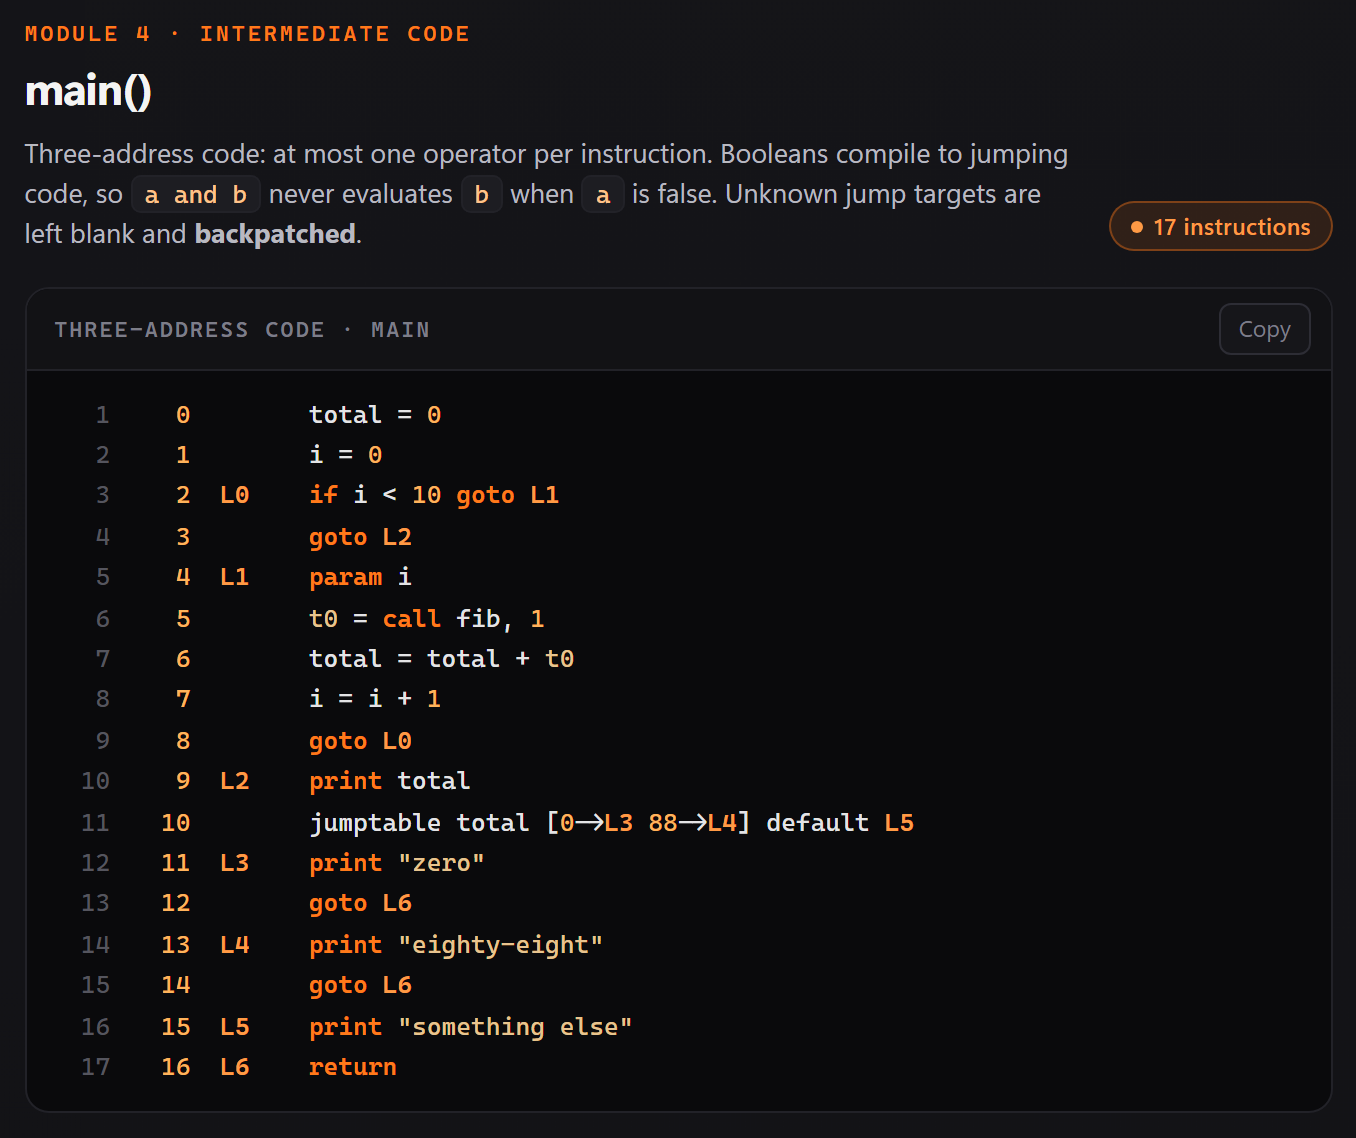
\includegraphics[width=\columnwidth]{figures/view-tac.png}
\caption{Three-address code for the main program of the Fibonacci benchmark: the loop as backpatched conditional jumps, and the \code{case} statement as a single jump table \code{[0$\to$L3, 88$\to$L4] default L5}.}
\label{fig:tac}
\end{figure}

\begin{figure}[!t]
\centering
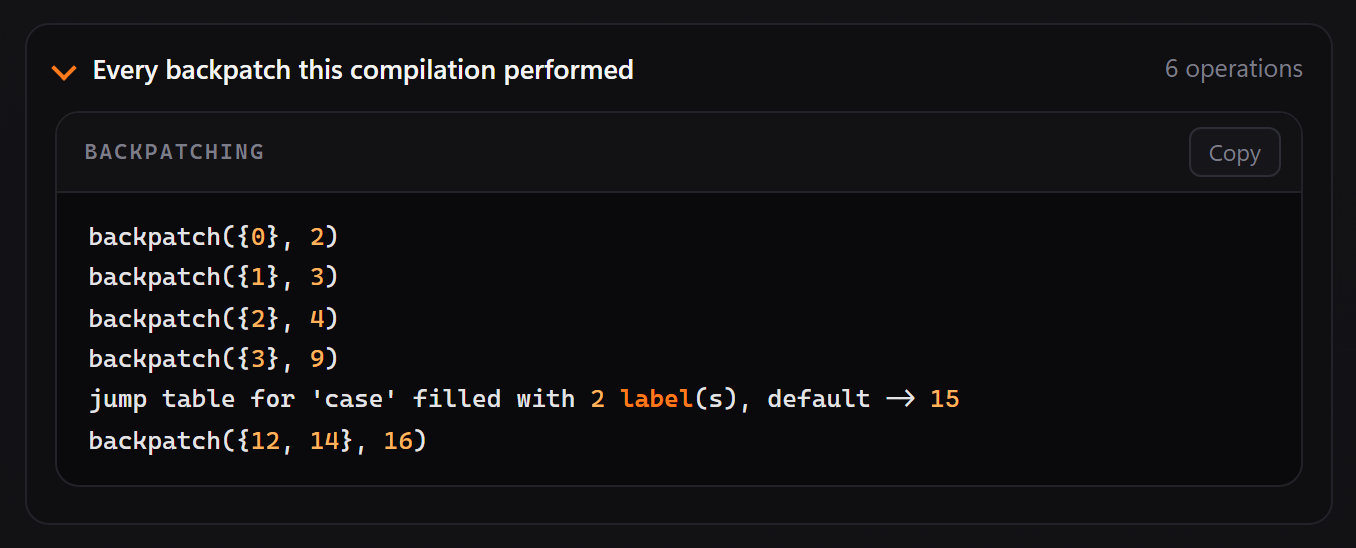
\includegraphics[width=\columnwidth]{figures/backpatch.png}
\caption{Every backpatch of the Fibonacci compilation: each line fills a list of pending jumps with the address that has just become known; the jump table of the \code{case} statement is filled with its two labels and its default.}
\label{fig:backpatch}
\end{figure}

\begin{figure}[!t]
\centering
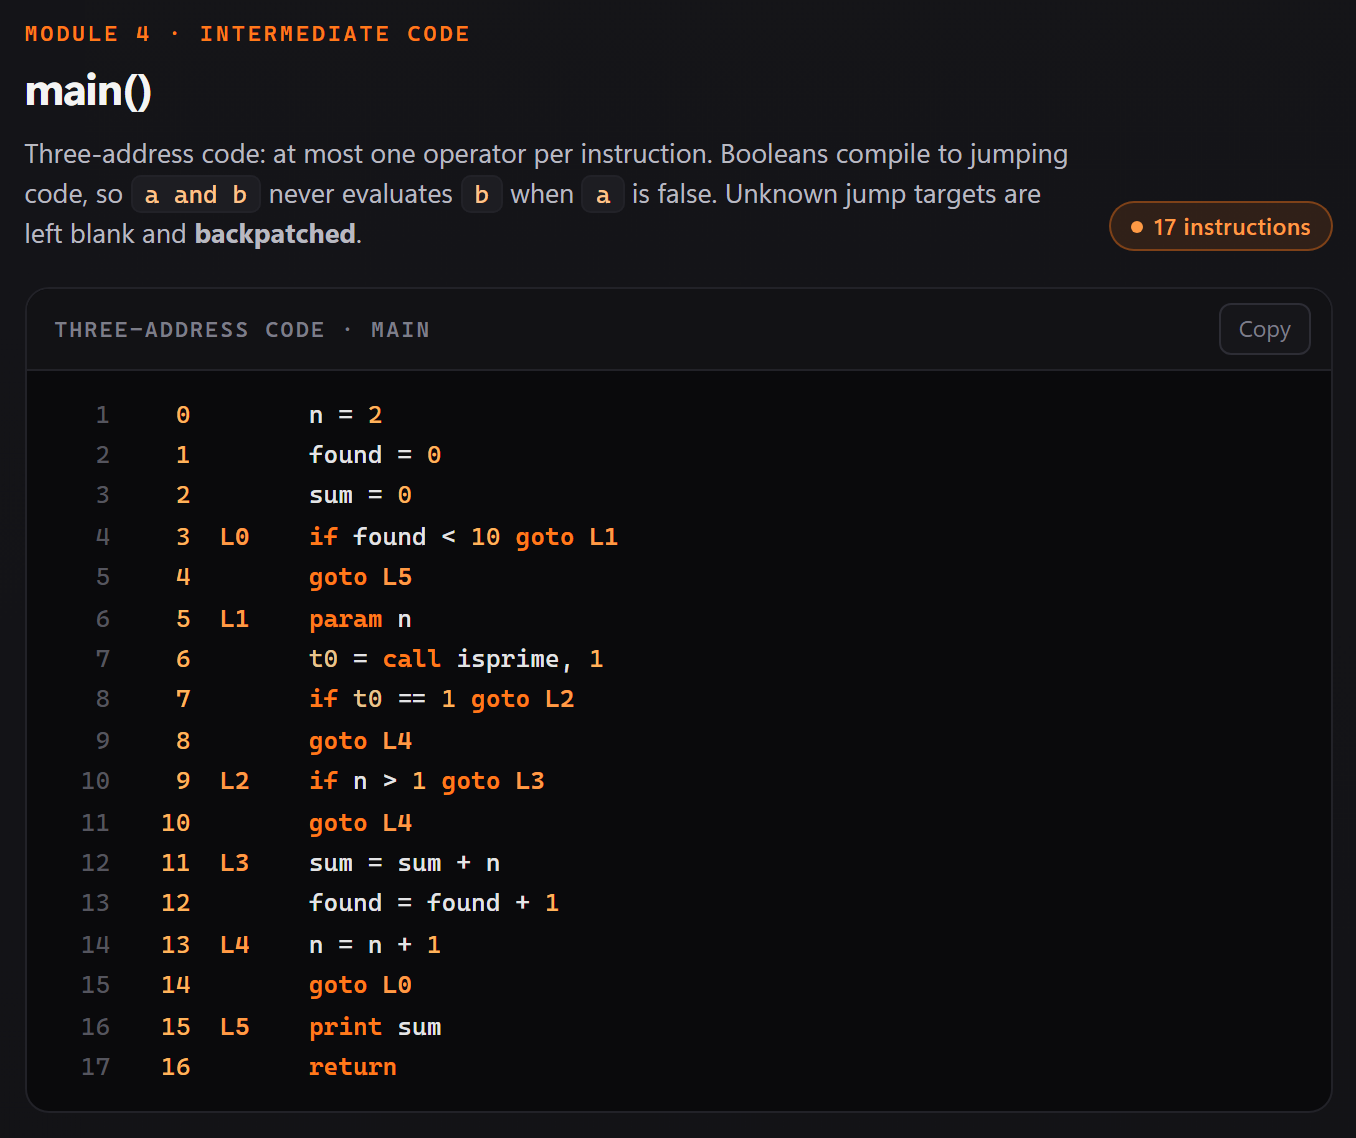
\includegraphics[width=\columnwidth]{figures/tac-primes.png}
\caption{Three-address code for the main program of \code{04\_primes.nova}. The condition \code{isprime(n) == 1 and n > 1} becomes two conditional jumps (instructions 7 and 9) whose false exits share the target \code{L4}: the jumping code of a short-circuit \code{and}.}
\label{fig:tacprimes}
\end{figure}

\subsection{Control Flow and Optimisation}
Leaders (the first instruction, every jump target and every instruction after a jump) delimit basic blocks, and the blocks form the control-flow graph (CFG). Inside the CFG every jump names a \emph{block} rather than an instruction index, so a pass may insert or delete instructions without invalidating jumps. Dominators are computed by iterative set intersection, immediate dominators are derived from them, and every back edge $n \to h$ with $h~\mathrm{dom}~n$ defines a natural loop. The optimiser runs eight passes in a fixed order and then repeats the first and the sixth as clean-up sweeps:
\begin{enumerate}
\item local value numbering and DAG construction (common subexpressions, constant folding, algebraic identities);
\item global constant propagation and
\item global copy propagation, both driven by reaching definitions;
\item loop-invariant code motion (LICM) into a synthesised preheader;
\item strength reduction of induction variables;
\item dead-code elimination driven by liveness;
\item unreachable-code elimination; and
\item jump optimisation.
\end{enumerate}
Each pass records the instruction count before and after it and the code it produced, which the studio plots as a waterfall (Fig.~\ref{fig:optimiser}). Flow graphs are drawn before and after optimisation (Fig.~\ref{fig:cfg}) in a layered layout in the manner of Sugiyama~\cite{sugiyama1981}: blocks are assigned to layers breadth-first from the entry, forward edges are cubic B\'ezier curves, and back edges are routed outside the blocks as dashed orange curves. The DAG of any block is drawn as well (Fig.~\ref{fig:dag}): leaves at the bottom, operators above their operands, each node annotated with the variables that hold its value, and nodes with more than one parent---the common subexpressions---outlined in orange. Fig.~\ref{fig:cfgprimes} shows a larger graph, \code{isprime} in \code{04\_primes.nova}, with eleven blocks: an early \code{return} for $n<2$, a loop whose header tests $d \cdot d \le n$, a second early \code{return} inside the loop body when a divisor is found, and the final \code{return 1}.

\begin{figure}[!t]
\centering
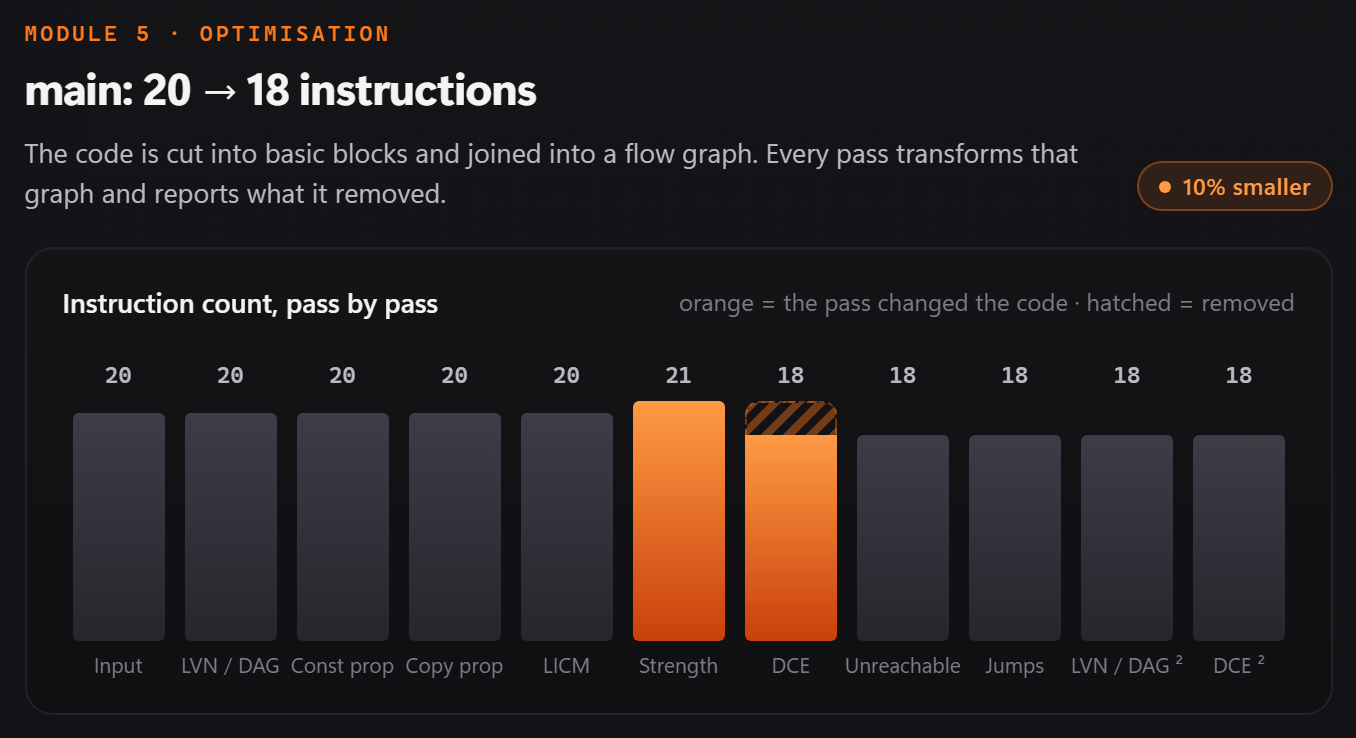
\includegraphics[width=\columnwidth]{figures/view-optimiser.png}
\caption{Optimiser view for \code{05\_optimiser.nova}: the instruction count of \code{main} after each pass. Orange bars changed the code; the hatched segment is removed code. Strength reduction temporarily adds an instruction; dead-code elimination then removes three.}
\label{fig:optimiser}
\end{figure}

\begin{figure*}[!t]
\centering
\subfloat[Before optimisation]{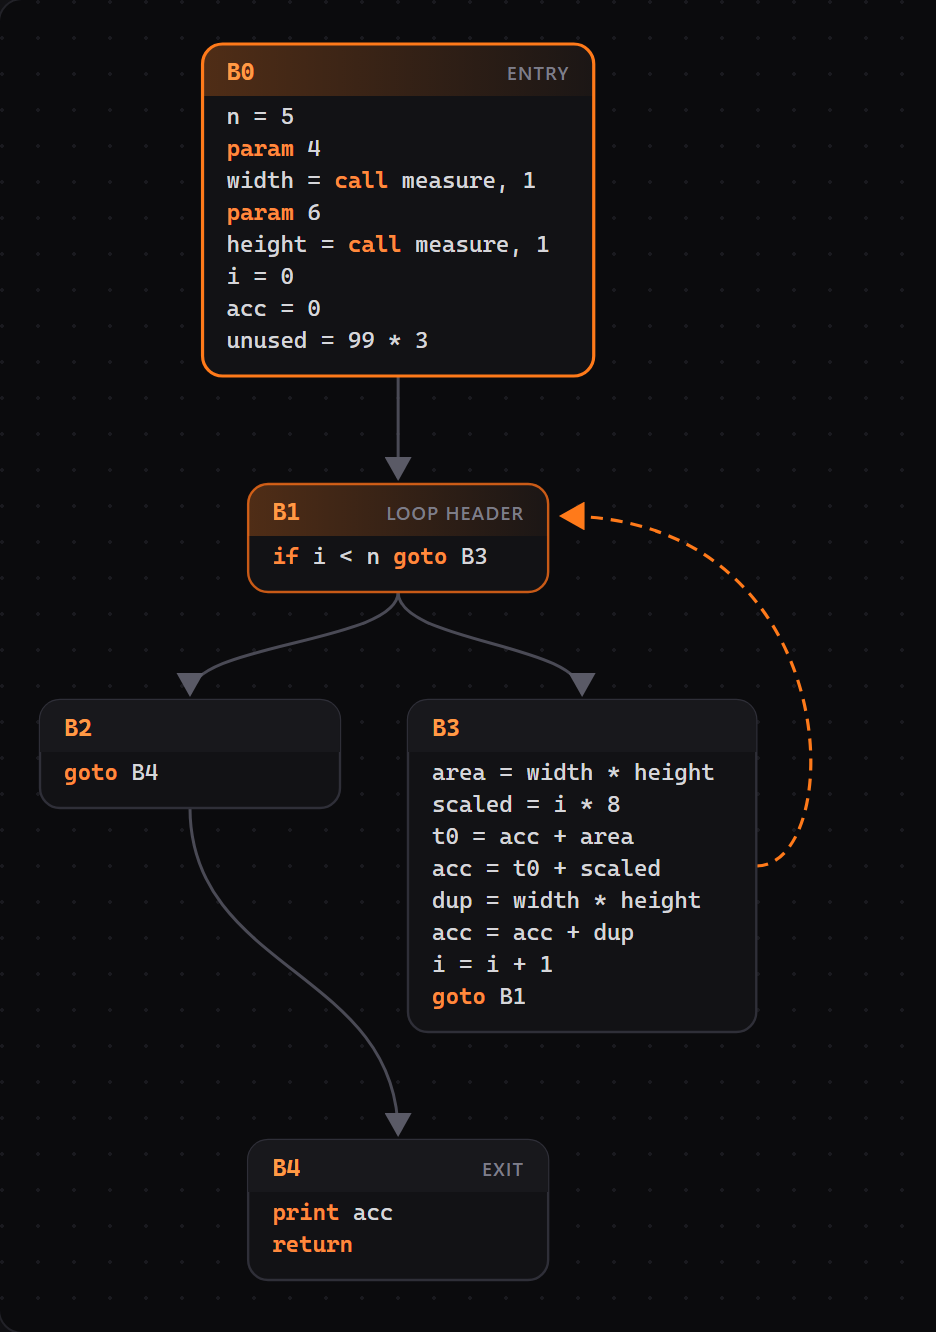
\includegraphics[height=7.2cm]{figures/cfg-before.png}\label{fig:cfg-before}}
\hspace{1.4cm}
\subfloat[After optimisation]{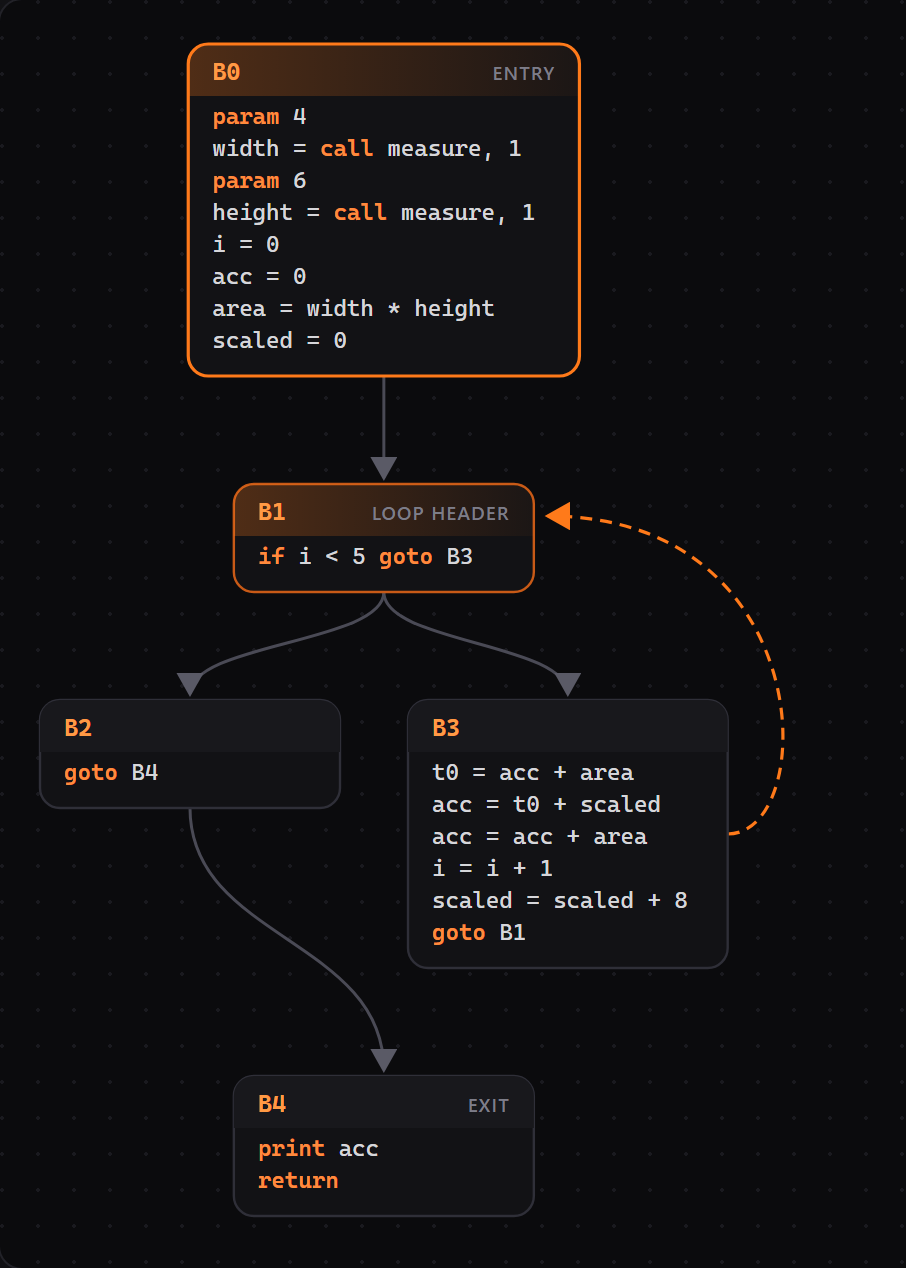
\includegraphics[height=6.85cm]{figures/cfg-after.png}\label{fig:cfg-after}}
\caption{Control-flow graphs of \code{main} in \code{05\_optimiser.nova}, rendered by the studio. Blocks are laid out in breadth-first layers from the entry. The entry, loop-header and exit blocks are labelled, and the dashed orange edge is the back edge that defines the loop. After optimisation, constant propagation has replaced \code{n} by \code{5} and its definition has gone, as has the never-read \code{unused}; the loop-invariant product \code{width*height} is computed once before the loop and reused instead of being recomputed as \code{dup}; and \code{scaled} is updated by addition (\code{scaled = scaled + 8}) instead of multiplication.}
\label{fig:cfg}
\end{figure*}

\begin{figure}[!t]
\centering
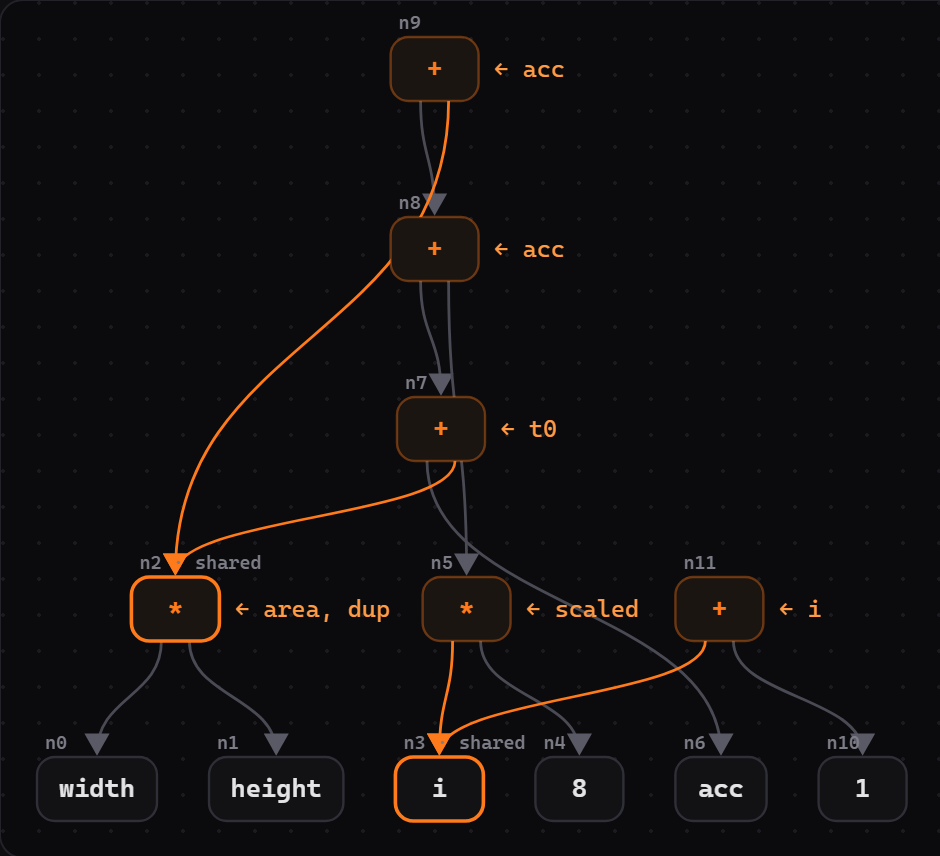
\includegraphics[width=0.9\columnwidth]{figures/dag.png}
\caption{The DAG of the loop body (\code{B3}) of \code{05\_optimiser.nova} before optimisation. Node \code{n2} (\code{width*height}) is shared by \code{area} and \code{dup}, which is how value numbering finds the common subexpression; the leaf \code{i} is shared by \code{scaled = i*8} and \code{i = i+1}. Orange edges lead to shared nodes.}
\label{fig:dag}
\end{figure}

\begin{figure}[!t]
\centering
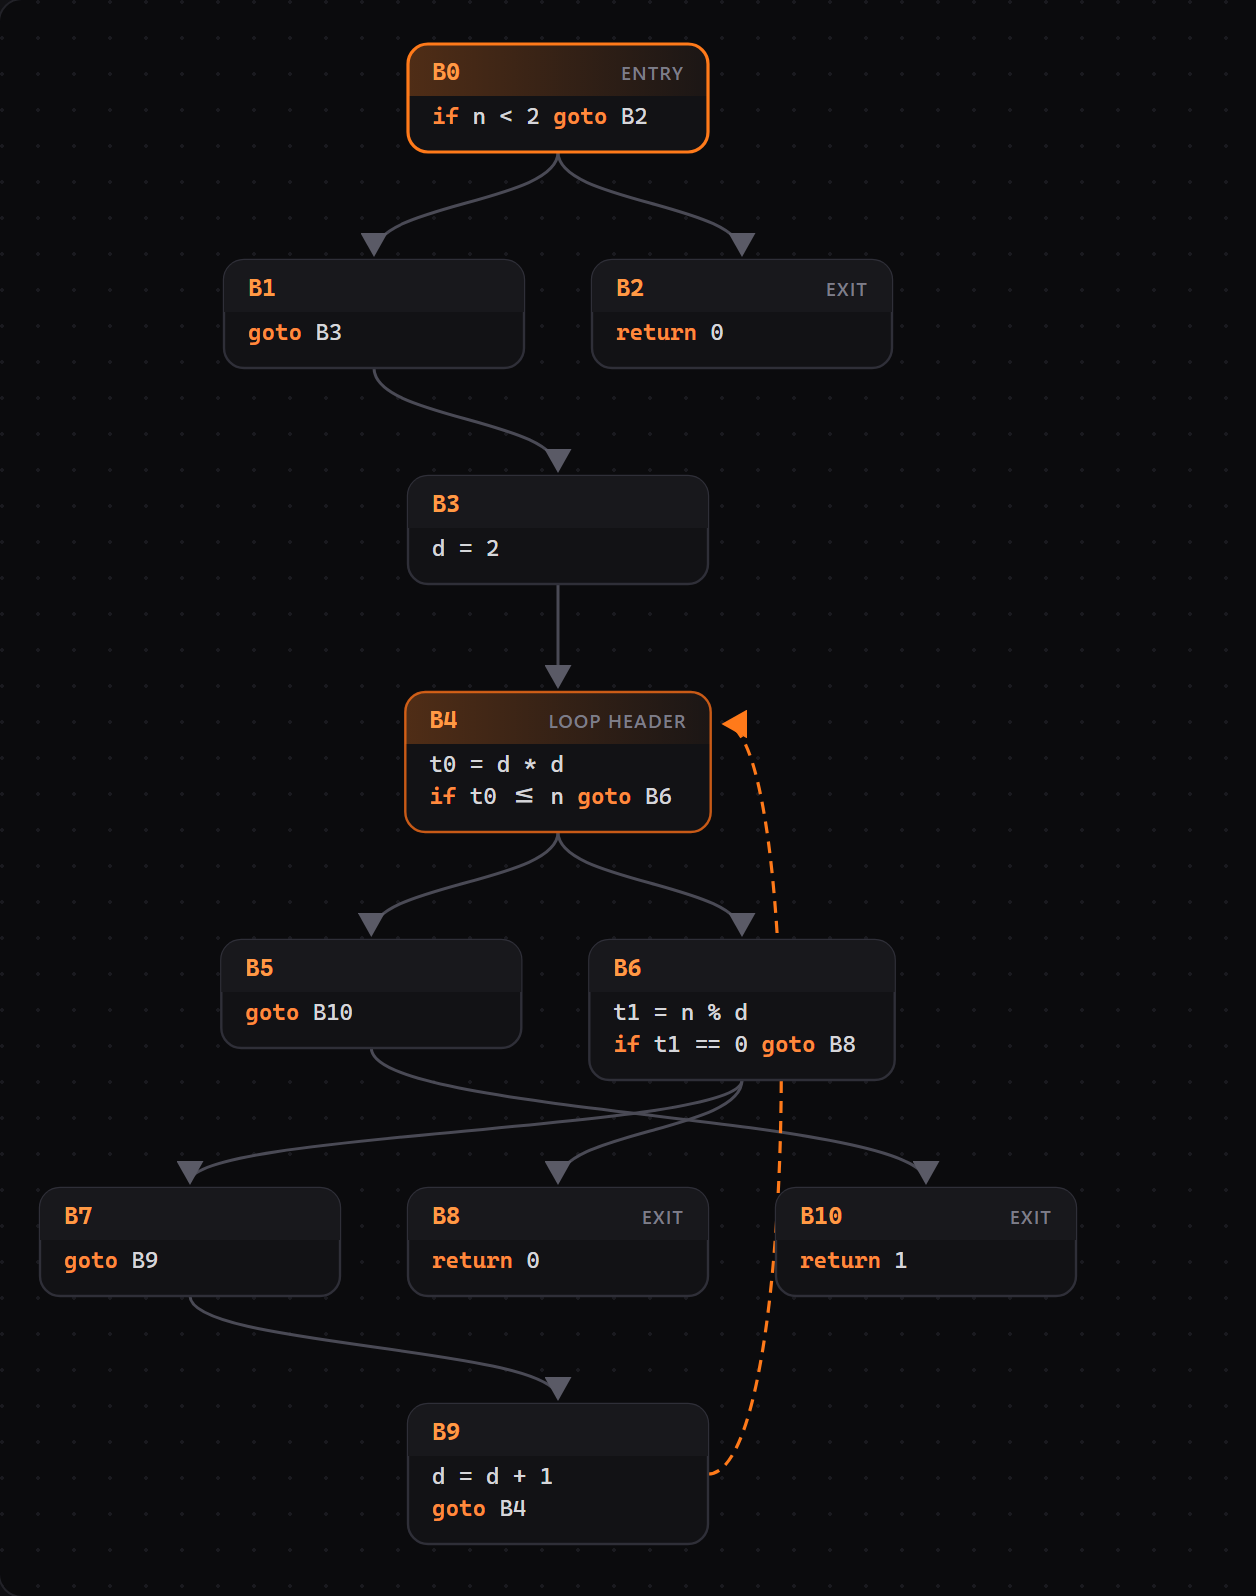
\includegraphics[width=0.8\columnwidth]{figures/cfg-primes.png}
\caption{The optimised flow graph of \code{isprime}: eleven blocks, three of them exits. The loop is headed by \code{B4} (the test $d \cdot d \le n$); its body \code{B6} contains the divisibility test whose true branch leaves the loop through the early \code{return} in \code{B8}, and the back edge from \code{B9} increments \code{d}.}
\label{fig:cfgprimes}
\end{figure}

\subsection{Data-Flow Analysis}
Four classical analyses are solved over the CFG in the monotone framework of Kildall~\cite{kildall1973}. With $\wedge$ the meet operator and $f_B$ the transfer function of block $B$, a forward analysis computes
\begin{equation}
\mathit{IN}[B] = \bigwedge_{P \in \mathrm{pred}(B)} \mathit{OUT}[P],\ \ \mathit{OUT}[B] = f_B(\mathit{IN}[B]),
\label{eq:forward}
\end{equation}
and a backward analysis computes
\begin{equation}
\mathit{OUT}[B] = \bigwedge_{S \in \mathrm{succ}(B)} \mathit{IN}[S],\ \ \mathit{IN}[B] = f_B(\mathit{OUT}[B]),
\label{eq:backward}
\end{equation}
with the instances listed in Table~\ref{tab:dataflow}. Reaching definitions drive constant and copy propagation, live variables drive dead-code elimination and register allocation, available expressions support global common-subexpression elimination, and very busy expressions justify code hoisting. Each analysis is solved by round-robin iteration over the blocks until no IN or OUT set changes, and a snapshot of every round is kept, so the convergence itself can be inspected (Fig.~\ref{fig:dataflow}). The studio also writes the final IN and OUT sets of the chosen analysis into the blocks of the flow graph (Fig.~\ref{fig:dfoverlay}), which places each fact next to the code it is a fact about. Figs.~\ref{fig:dfreaching} and~\ref{fig:dfavailable} show two further analyses on \code{main} of \code{05\_optimiser.nova}. In reaching definitions each definition is named by its variable and its position---\code{acc@B0.6} is the definition of \code{acc} at instruction 6 of \code{B0}---and the sets at the loop header contain the definitions from both the entry block and the loop body, because the meet is union. Available expressions behaves the opposite way: the loop body computes \code{width*height}, \code{i+1} and the other expressions, so they are available at its exit, but at the header they are intersected with the entry path, which has computed none of them, and only \code{99*3} survives.

\begin{table}[!t]
\caption{The Four Data-Flow Analyses}
\label{tab:dataflow}
\centering
\footnotesize
\setlength{\tabcolsep}{3.5pt}
\begin{tabular}{@{}l c c l@{}}
\toprule
Analysis & Direction & $\wedge$ & Transfer $f_B(x)$ \\
\midrule
Reaching definitions & forward & $\cup$ & $\mathit{gen}_B \cup (x - \mathit{kill}_B)$ \\
Live variables & backward & $\cup$ & $\mathit{use}_B \cup (x - \mathit{def}_B)$ \\
Available expressions & forward & $\cap$ & $\mathit{egen}_B \cup (x - \mathit{ekill}_B)$ \\
Very busy expressions & backward & $\cap$ & $\mathit{euse}_B \cup (x - \mathit{ekill}_B)$ \\
\bottomrule
\end{tabular}
\end{table}

\begin{figure}[!t]
\centering
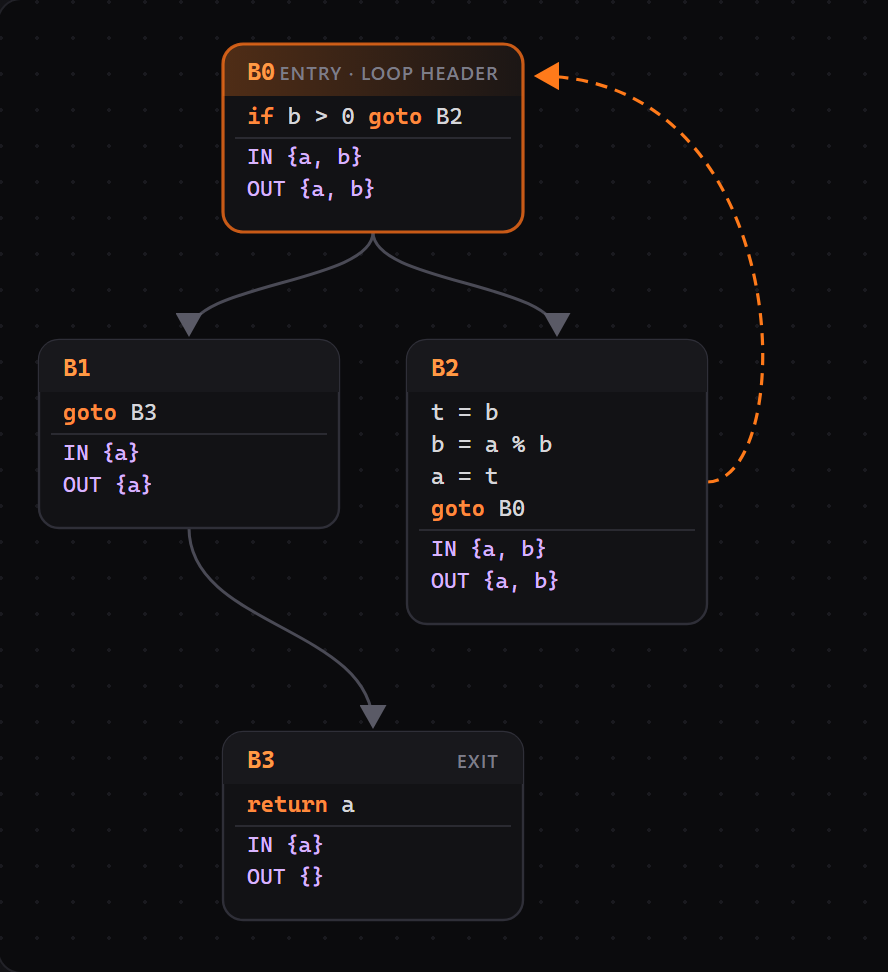
\includegraphics[width=0.9\columnwidth]{figures/df-overlay.png}
\caption{Live-variable facts written onto the flow graph of \code{gcd}: both \code{a} and \code{b} are live into the loop header and through the loop body, only \code{a} is live on the exit path, and nothing is live after \code{return}.}
\label{fig:dfoverlay}
\end{figure}

\begin{figure}[!t]
\centering
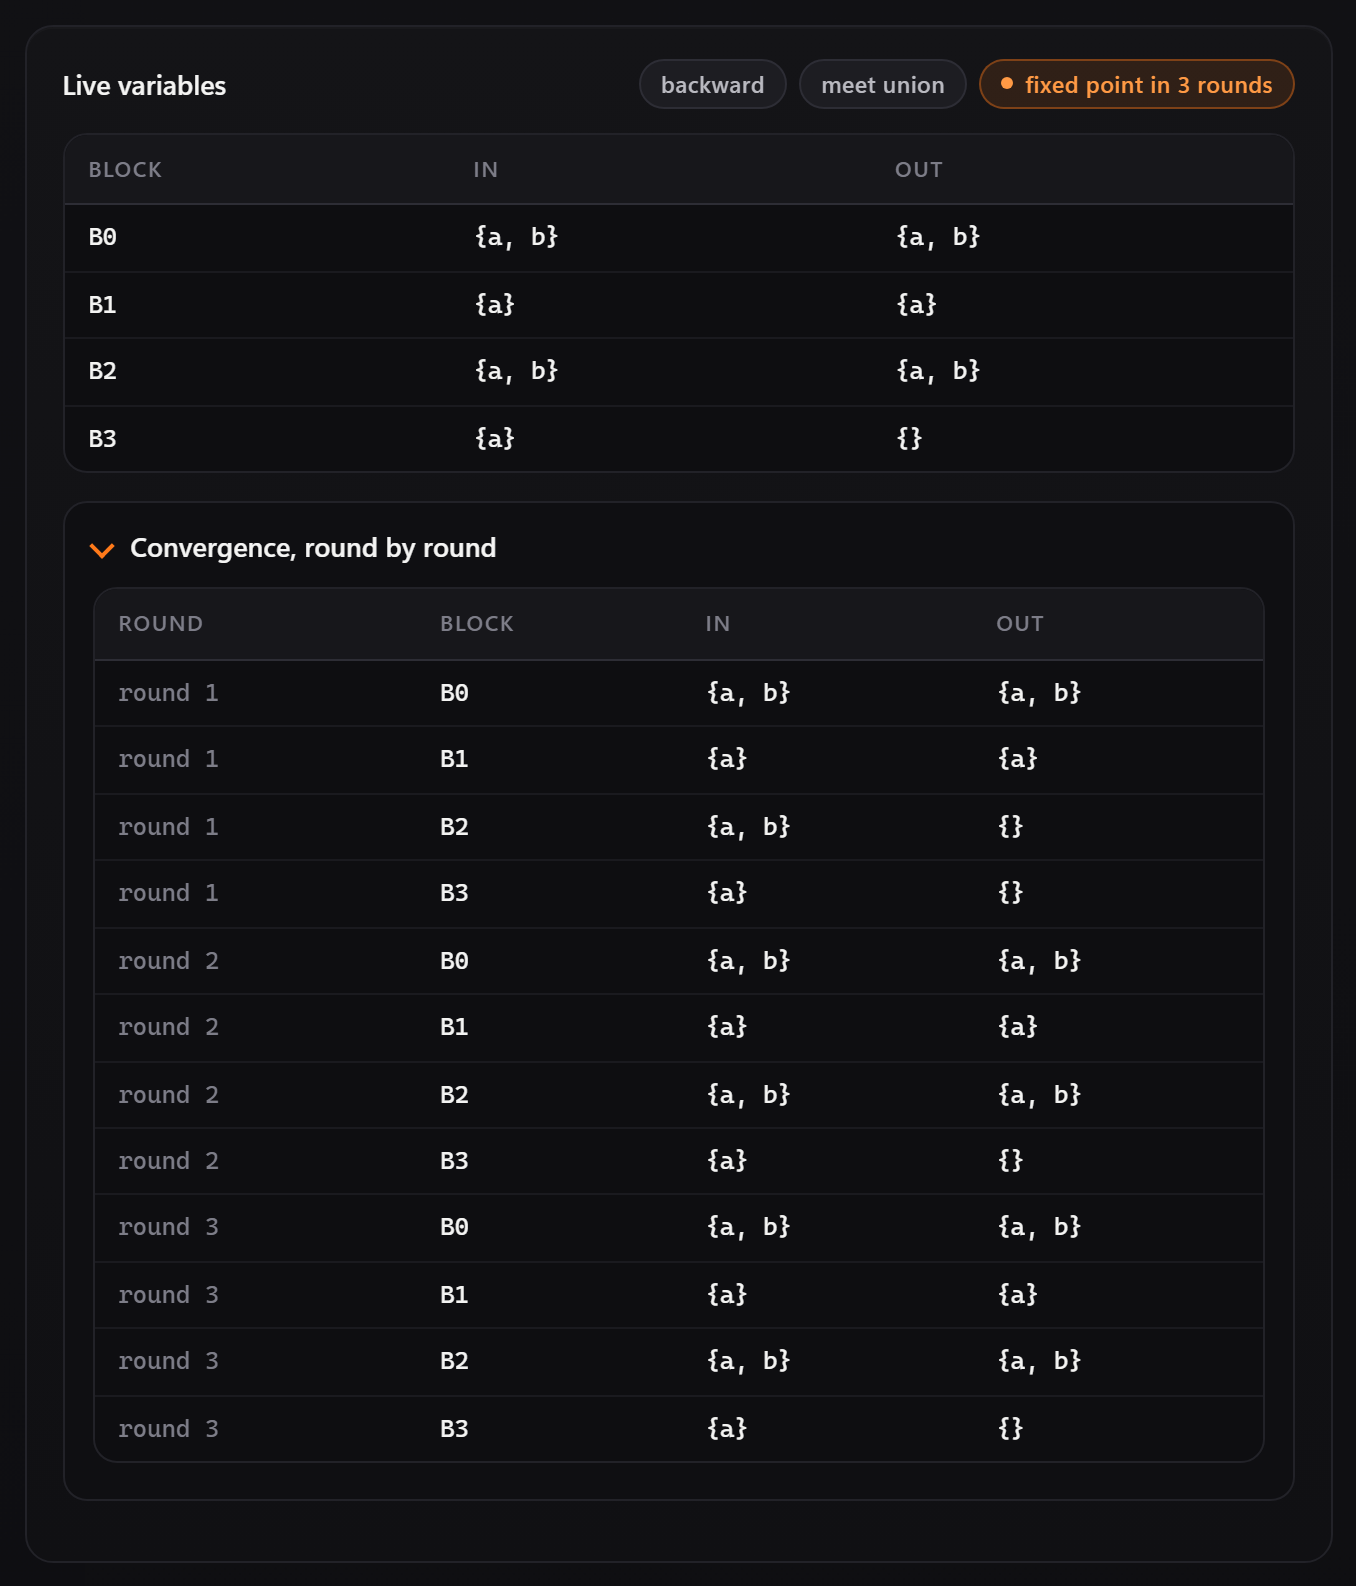
\includegraphics[width=0.92\columnwidth]{figures/view-dataflow.png}
\caption{Live-variable analysis of \code{gcd}: the final IN/OUT sets and the convergence table. \code{B2}'s OUT set is empty after round 1 and becomes $\{a, b\}$ in round 2 once the loop's back edge has propagated it; round 3 confirms the fixed point.}
\label{fig:dataflow}
\end{figure}

\begin{figure}[!t]
\centering
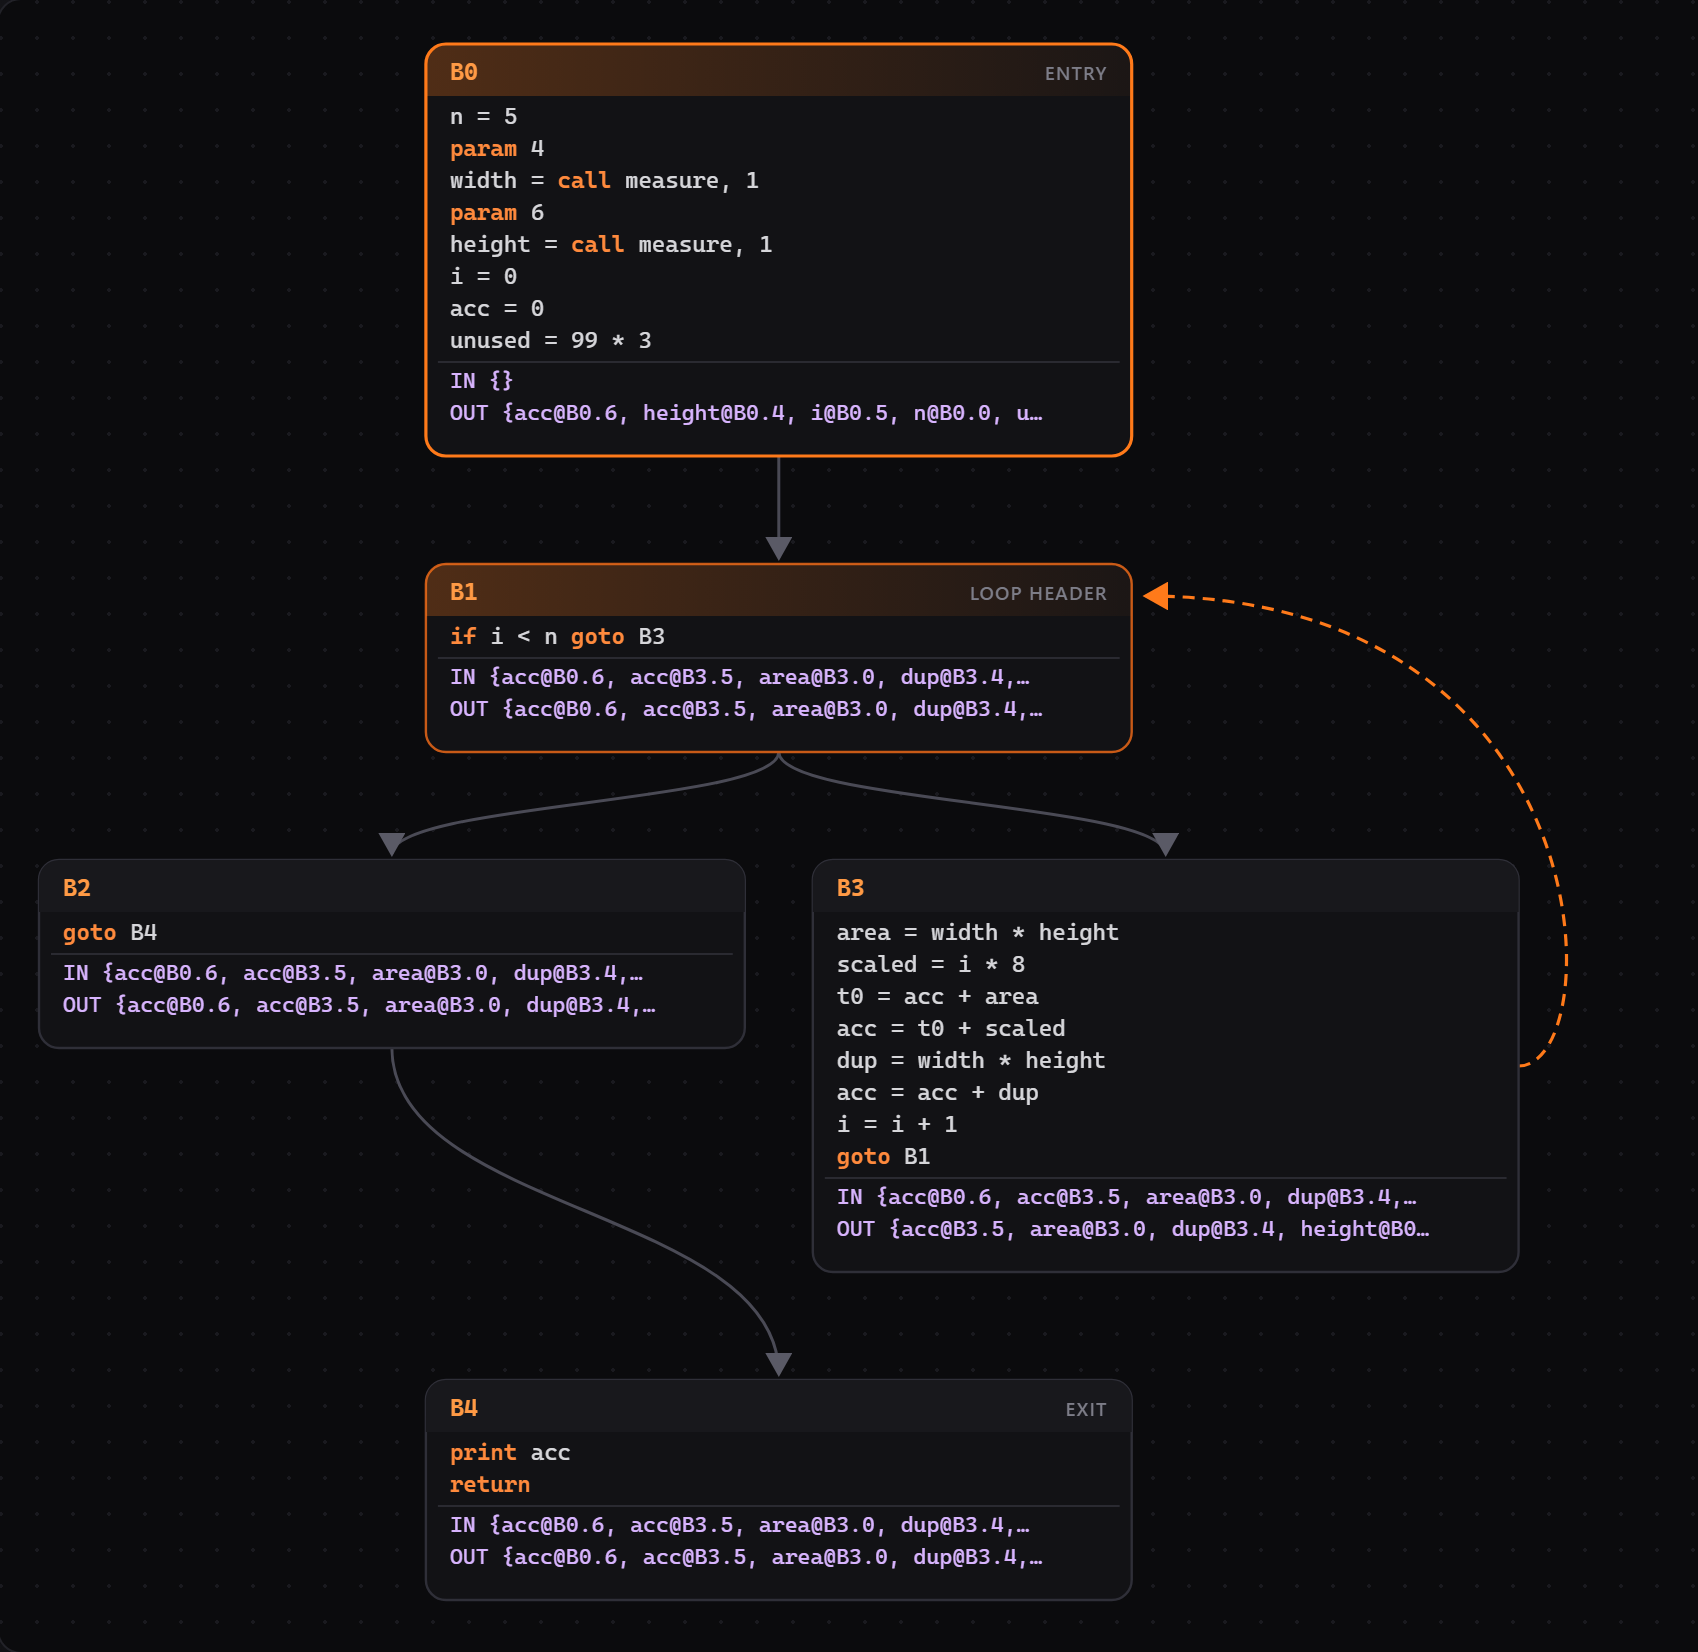
\includegraphics[width=0.92\columnwidth]{figures/df-reaching.png}
\caption{Reaching definitions on the flow graph of \code{main} in \code{05\_optimiser.nova} before optimisation. Every definition in \code{B0} and \code{B3} reaches the loop header \code{B1}, so the facts at \code{B1}, \code{B2} and \code{B4} name definitions from both blocks; the studio truncates long sets with an ellipsis and shows them in full in the table below the graph.}
\label{fig:dfreaching}
\end{figure}

\begin{figure}[!t]
\centering
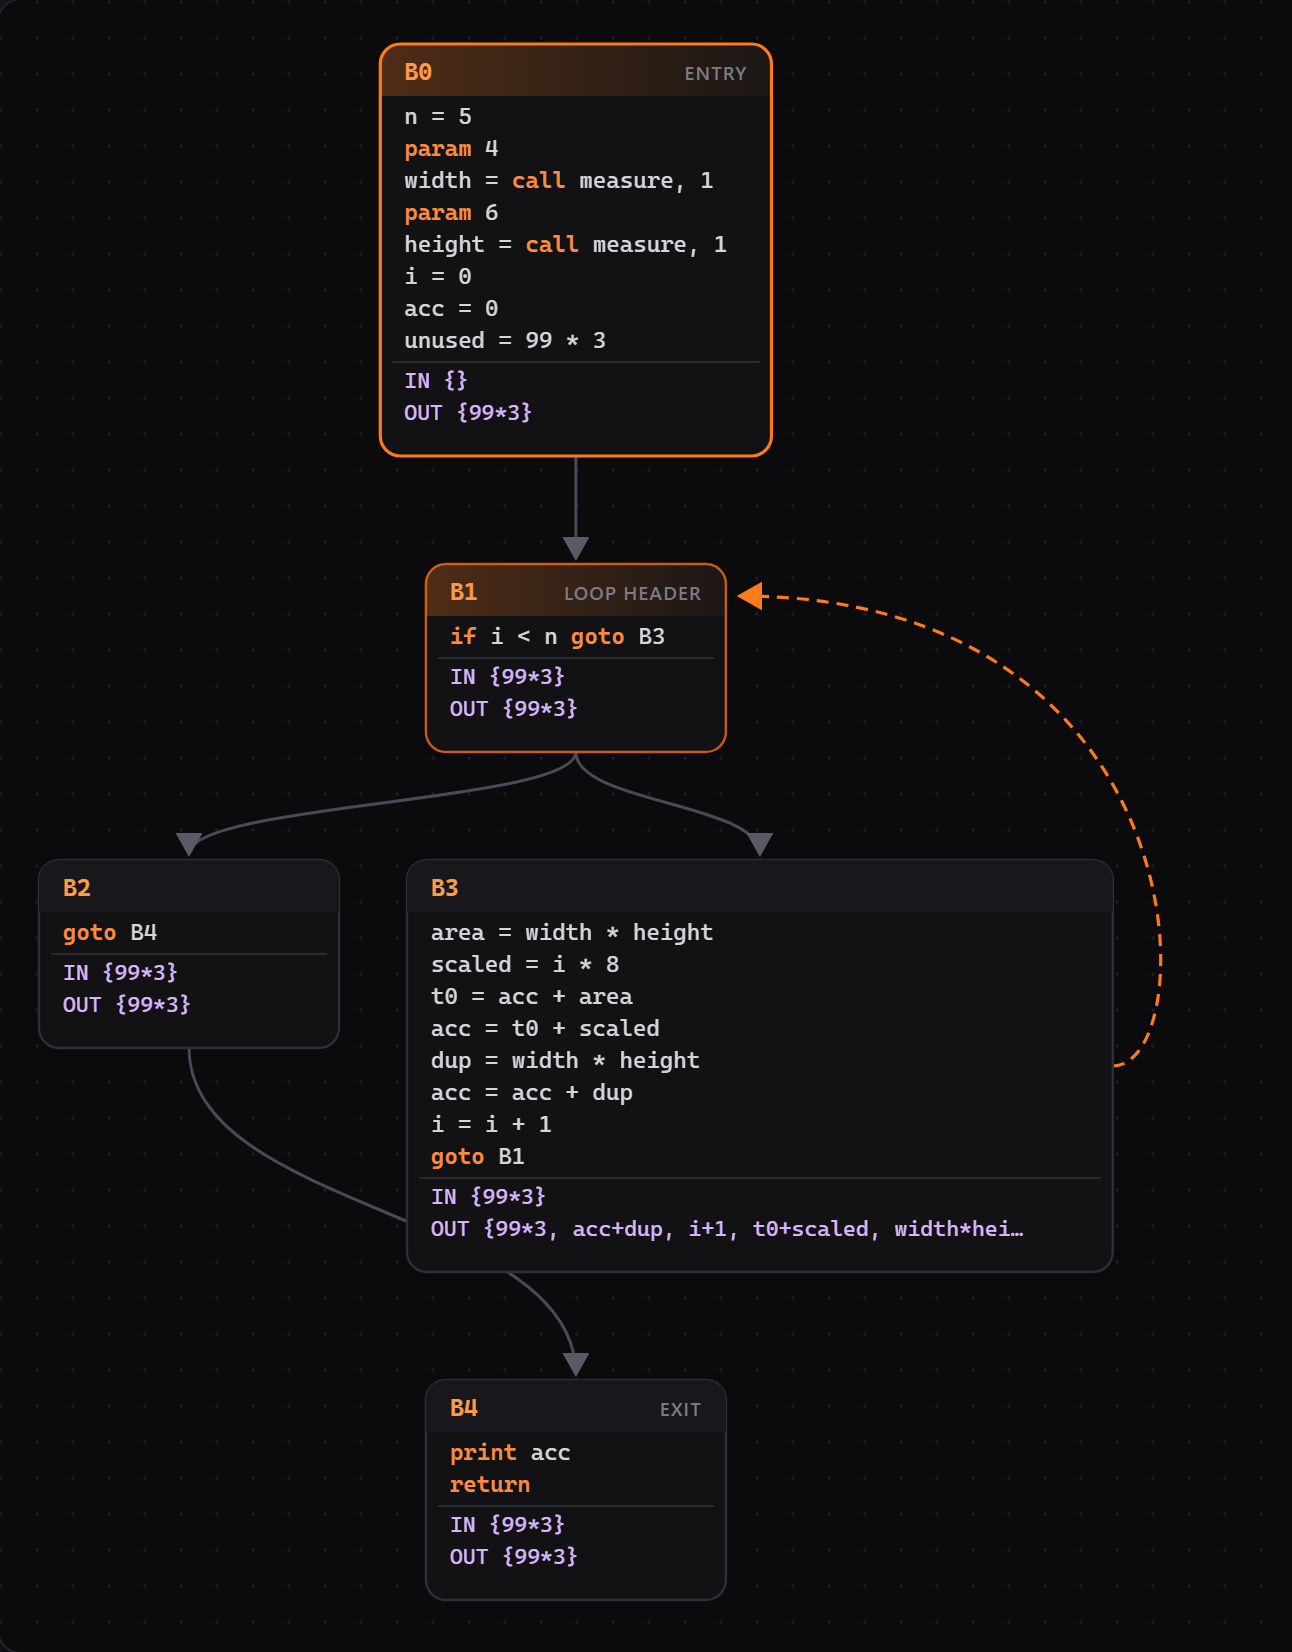
\includegraphics[width=0.82\columnwidth]{figures/df-available.png}
\caption{Available expressions on the same graph. The loop body \code{B3} makes \code{acc+dup}, \code{i+1}, \code{t0+scaled}, \code{width*height} and others available at its exit, but the meet at the loop header is intersection with the entry path, so only \code{99*3}, computed in \code{B0}, is available on every path into \code{B1}.}
\label{fig:dfavailable}
\end{figure}

\subsection{Code Generation and Register Allocation}
The register code generator implements the textbook simple code generator over four general-purpose registers. A backward scan of each block computes, for every instruction, the next use and liveness of each name, starting from the block's live-out set. The register-selection routine \code{getreg} chooses, in order: an empty register; a register whose value is dead; or a register to spill, chosen by Belady's rule~\cite{belady1966},
\begin{equation}
r^{*} = \arg\max_{r}\ \mathit{nextuse}\bigl(v(r)\bigr),
\label{eq:belady}
\end{equation}
where $v(r)$ is the value held in register $r$. A register descriptor (what each register holds) and an address descriptor (where each value lives) are recorded after every instruction (Fig.~\ref{fig:regdec}), and values that are live at a block's exit are stored to their slots in the activation record, so that blocks can be generated independently. The activation record holds the return address at offset $-2$, the control link at $-1$, then parameters, locals and temporaries (Fig.~\ref{fig:codegen}). A register-machine simulator executes the generated code, which turns the code listing into a working back-end. The studio turns the register descriptors into a timeline (Fig.~\ref{fig:timeline}): one row per register, one column per instruction, a coloured run for every interval during which a value occupies a register, so that the allocator's reuse of registers and its spills can be read at a glance. The next-use table (Fig.~\ref{fig:nextuse}) is the input to those decisions: for each instruction it lists, for every name involved, the index of its next use within the block or \code{live-out} when the value survives the block, and the set of names that are live after the instruction.

\begin{figure*}[!t]
\centering
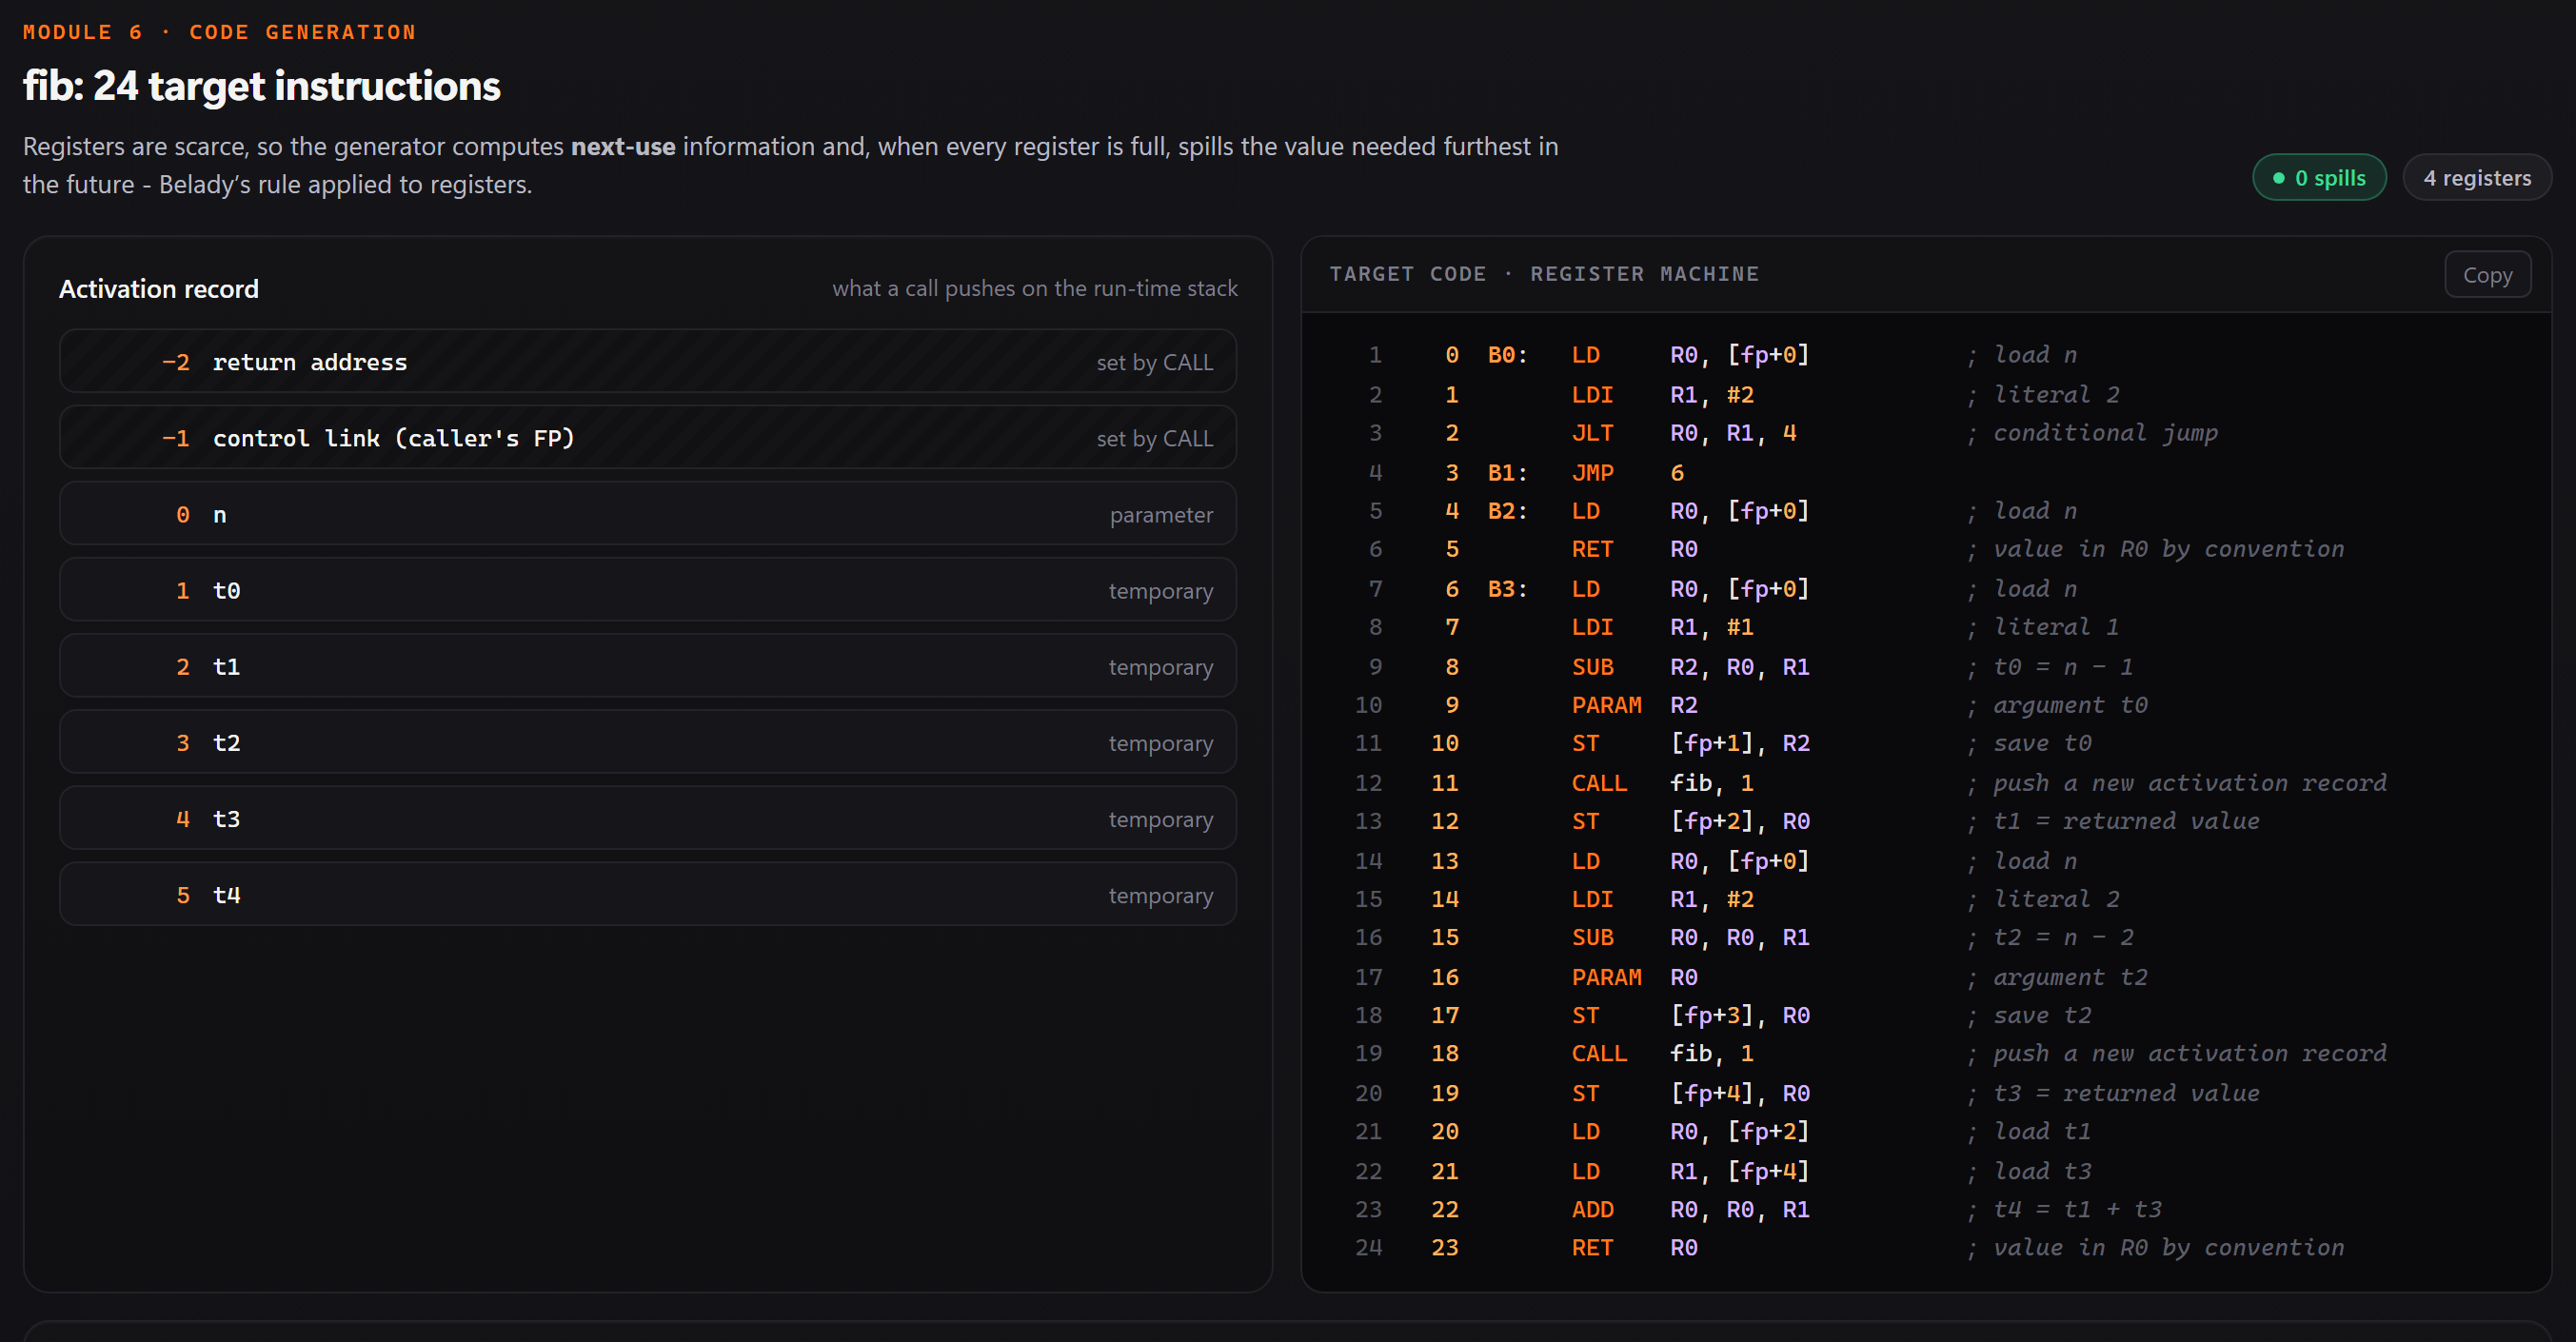
\includegraphics[width=0.94\textwidth]{figures/view-codegen.png}
\caption{Code-generation view for the recursive function \code{fib}: the activation-record layout (left) and the 24-instruction register-machine code (right), with the allocator's comment on each instruction. No spills are needed with four registers.}
\label{fig:codegen}
\end{figure*}

\begin{figure*}[!t]
\centering
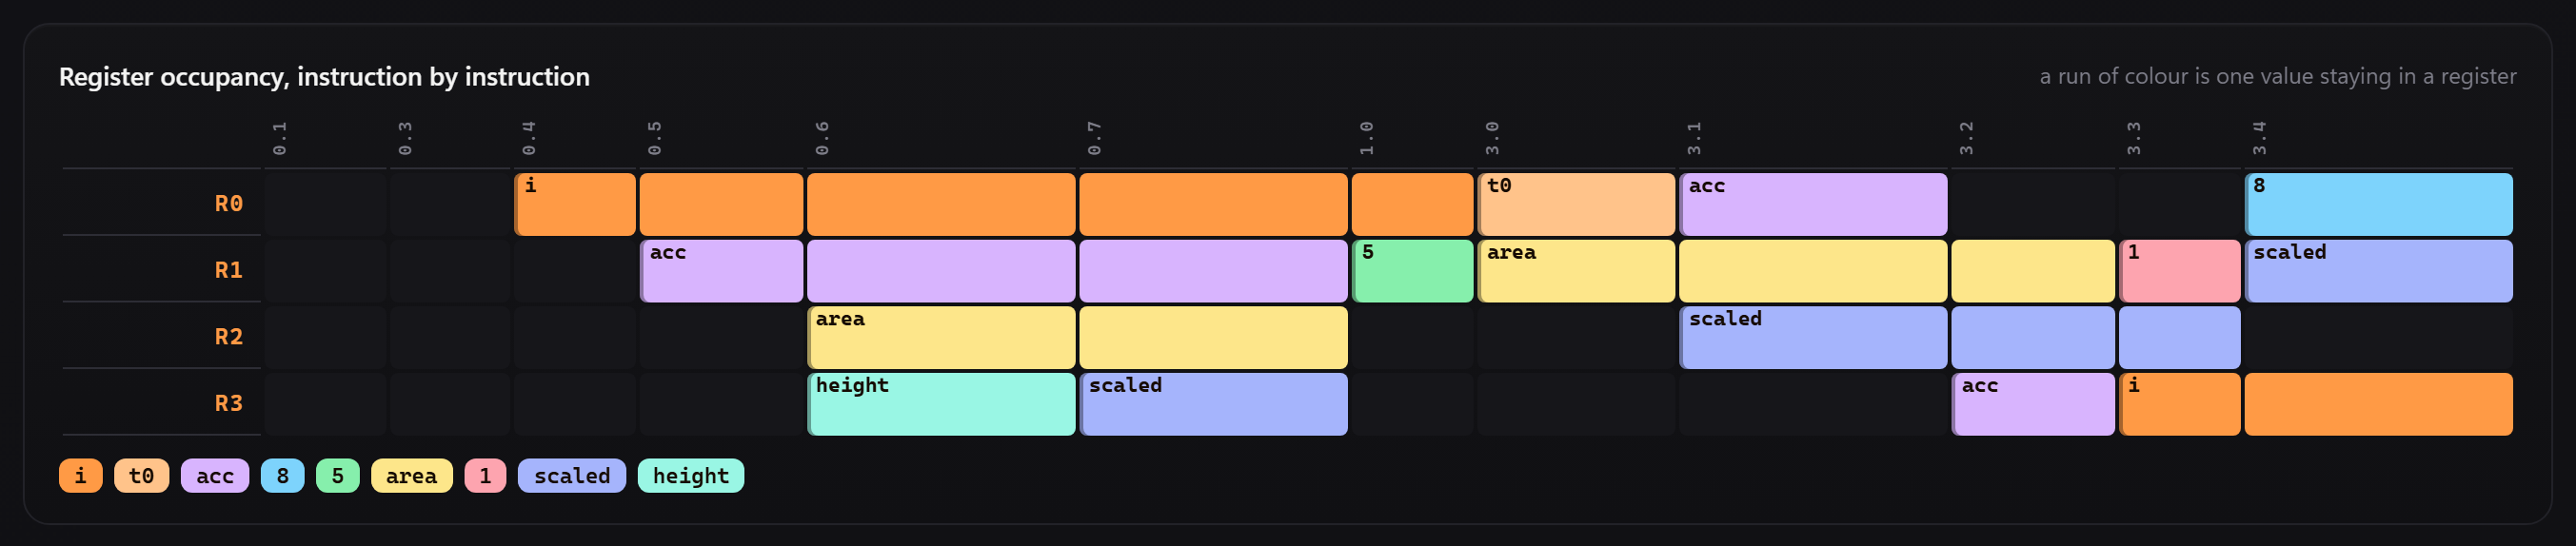
\includegraphics[width=0.94\textwidth]{figures/reg-timeline.png}
\caption{Register occupancy for \code{main} of \code{05\_optimiser.nova}, instruction by instruction. Each coloured run is one value held in one register; \code{i} stays in \code{R0} through the whole entry block, \code{area} moves from \code{R2} to \code{R1} between blocks because every block is generated independently, and the constants \code{5}, \code{1} and \code{8} occupy registers only for the instruction that needs them.}
\label{fig:timeline}
\end{figure*}

\begin{figure*}[!t]
\centering
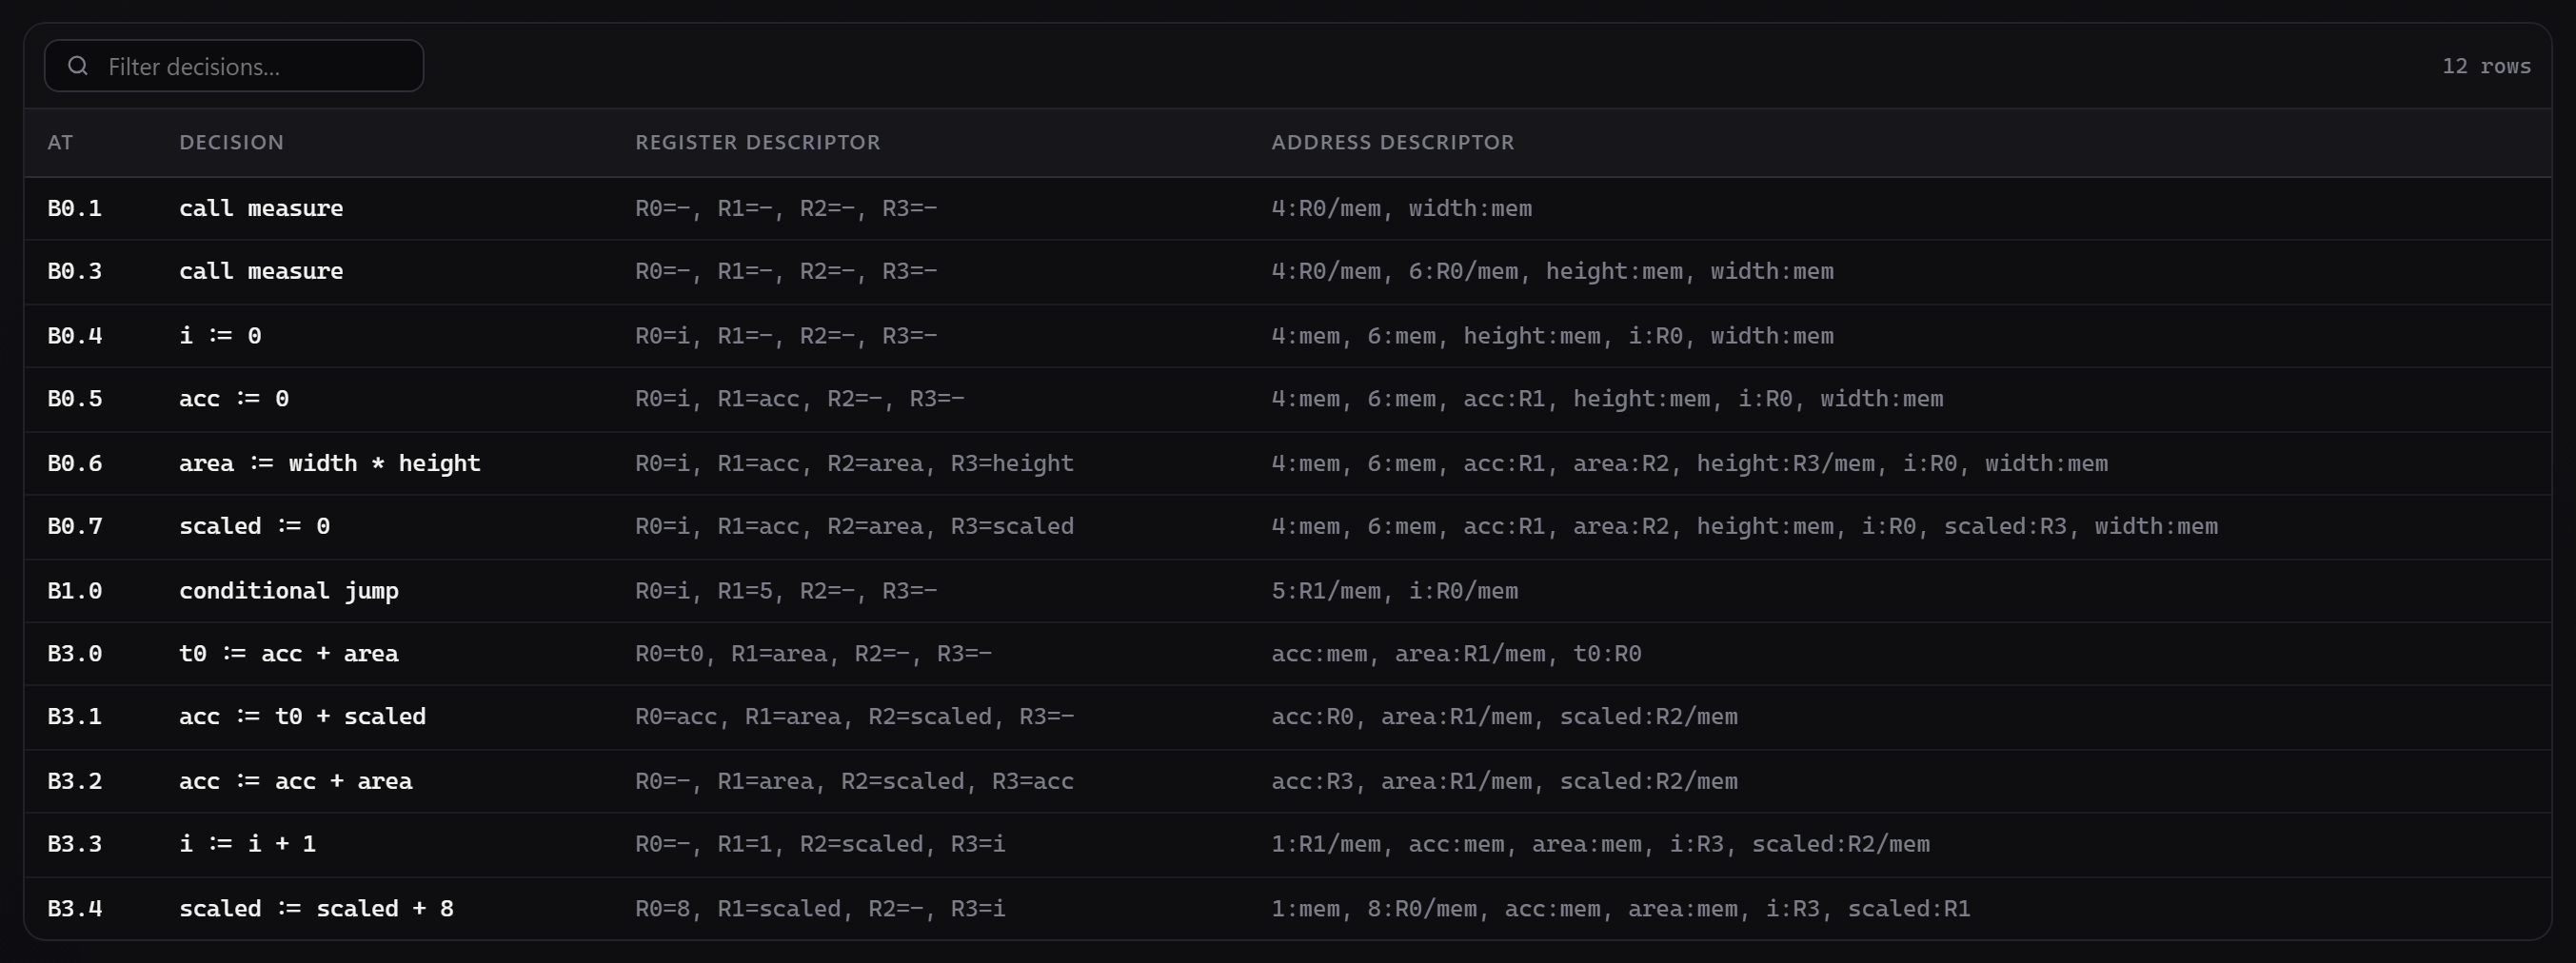
\includegraphics[width=0.94\textwidth]{figures/reg-decisions.png}
\caption{The allocator's decisions for \code{main} of \code{05\_optimiser.nova}: after every instruction, the register descriptor (what each register holds) and the address descriptor (where every value currently lives---a register, memory or both). At \code{B3.0}, for example, \code{t0} is created in \code{R0} while \code{area} lives in both \code{R1} and memory.}
\label{fig:regdec}
\end{figure*}

\begin{figure*}[!t]
\centering
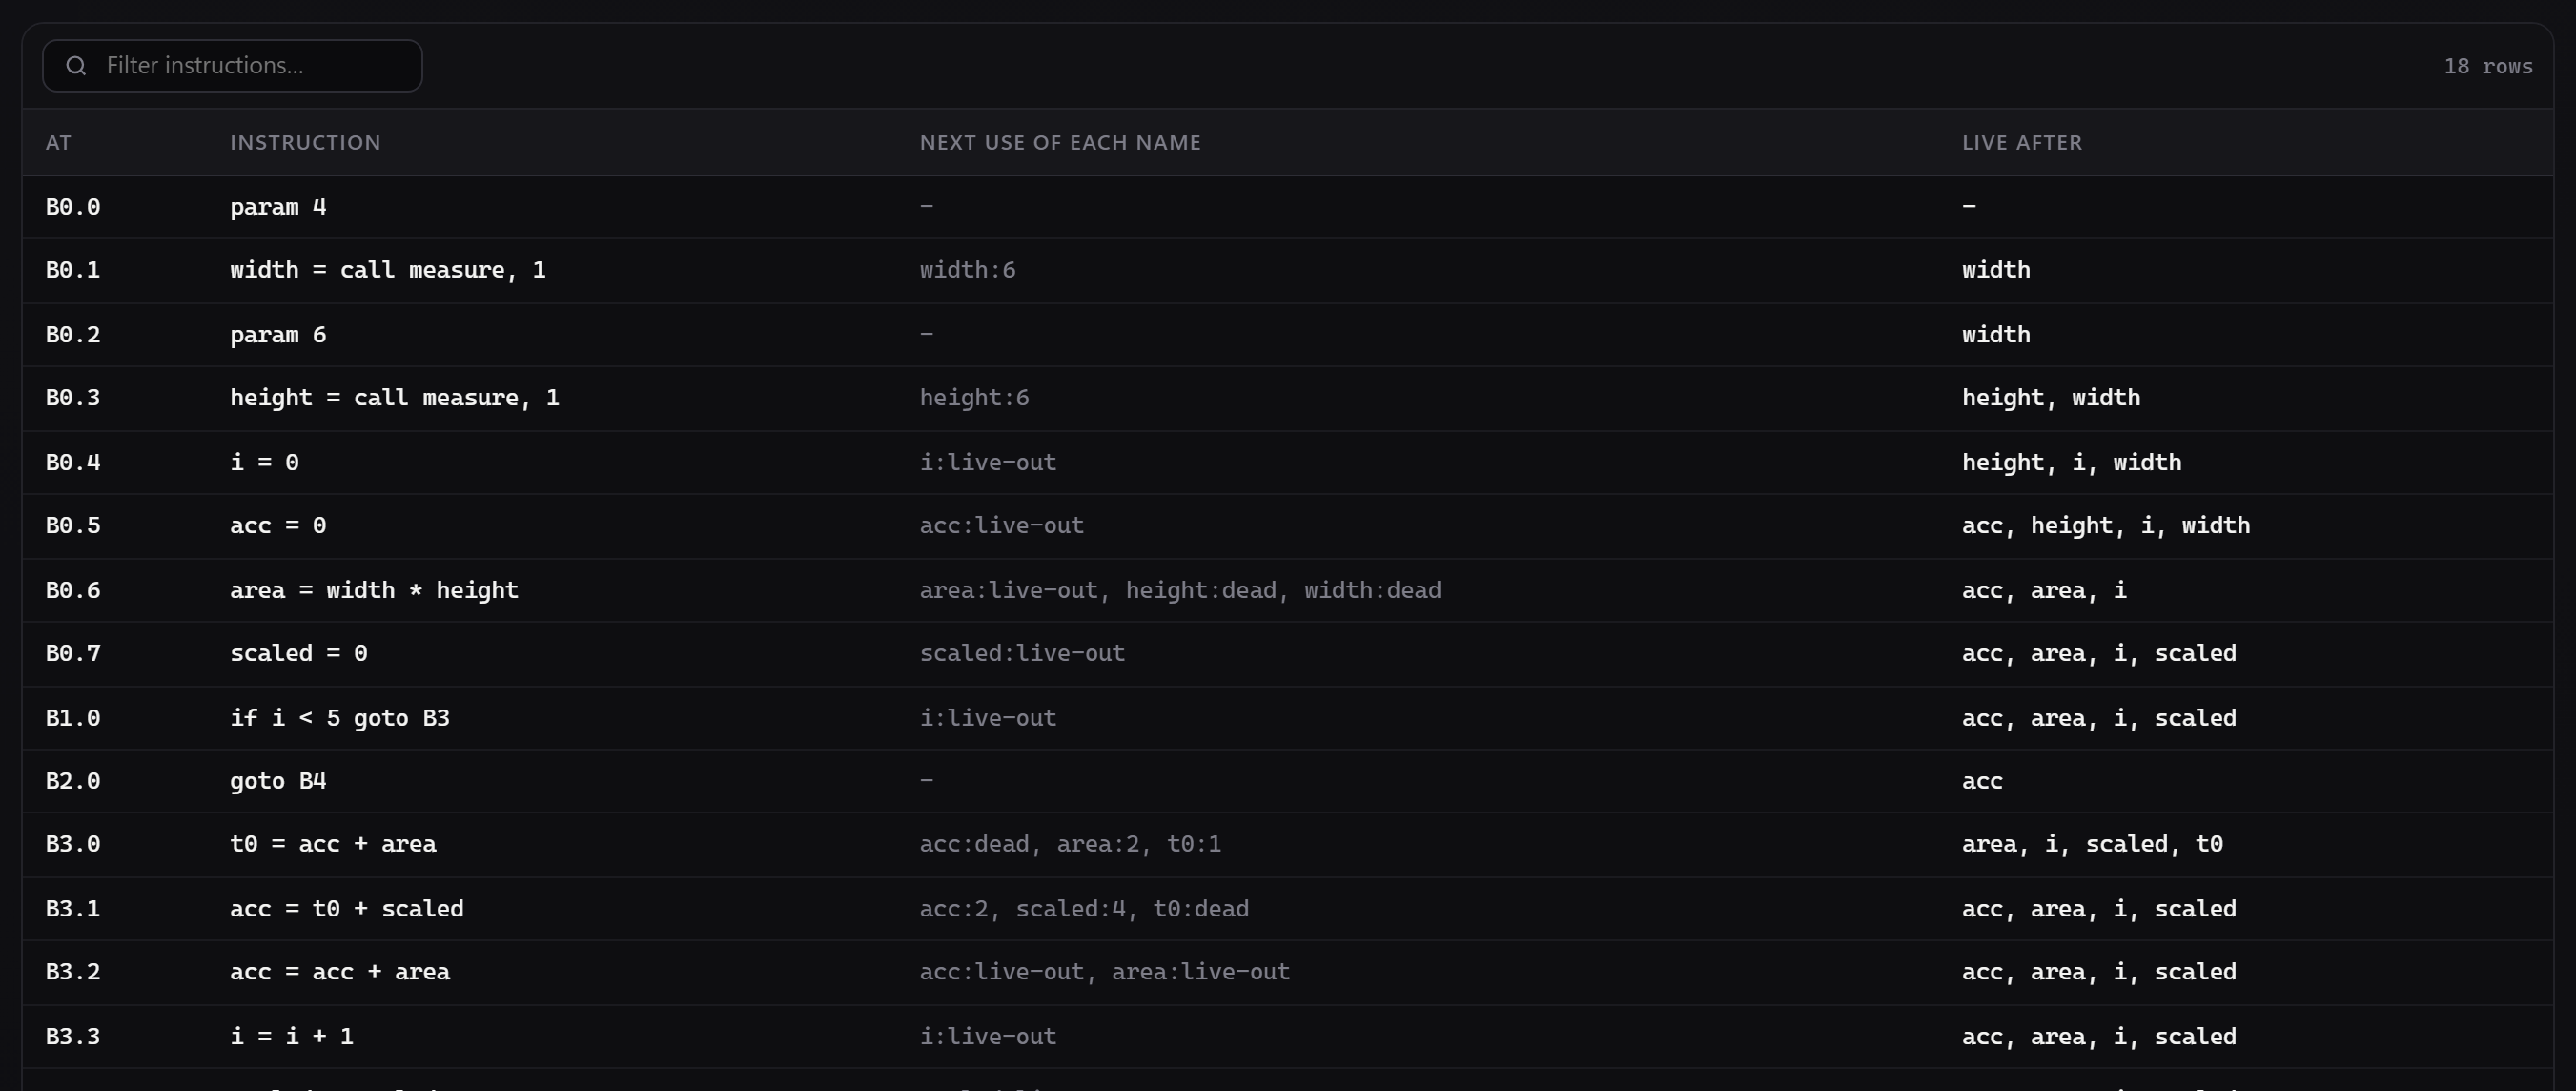
\includegraphics[width=0.94\textwidth]{figures/nextuse.png}
\caption{Next-use information for \code{main} of \code{05\_optimiser.nova}, the first 14 instructions. Each row gives the instruction, the next use of every name it touches (an instruction index within the block, \code{live-out}, or \code{dead}) and the names live after it; \code{getreg} spills the register whose value has the most distant next use.}
\label{fig:nextuse}
\end{figure*}

\subsection{SSA Construction and Parallelism}
SSA form is built by the method of Cytron~\emph{et~al.}~\cite{cytron1991}. The dominance frontier of block $n$ is
\begin{equation}
\mathrm{DF}(n)=\{\,y \mid \exists p\in\mathrm{pred}(y): n~\mathrm{dom}~p \;\wedge\; \neg(n~\mathrm{sdom}~y)\,\},
\label{eq:df}
\end{equation}
computed by walking up the dominator tree from the predecessors of each join block. The entry block is treated as having an extra, implicit predecessor---the function's start---so a loop that begins at the very first instruction is still recognised as a join (Section~\ref{sec:res-defects}). $\phi$-functions are placed on the iterated dominance frontier of each variable's definition sites, and variables are renamed in a pre-order walk of the dominator tree using one version stack per variable (Fig.~\ref{fig:ssa}). The dominator tree itself is drawn, with each block's dominance frontier beside it (Fig.~\ref{fig:domtree}). Fig.~\ref{fig:ssaprimes} shows the SSA form of \code{isprime}: its loop header \code{B4} receives three $\phi$-functions, for \code{d} and for the two temporaries that the loop body redefines. Fig.~\ref{fig:domparallel} shows the dominator tree of \code{main} in \code{06\_parallel.nova}: a chain through the three loop headers \code{B1}, \code{B5} and \code{B9}, each of which is in its own dominance frontier and in that of its loop body (\code{B3}, \code{B7}, \code{B11}).

For every natural loop, the dependence analyser computes four sets of variables:
\begin{itemize}
\item $W$, those written in the loop;
\item $U$, the upward-exposed reads (read before being written in an iteration);
\item $I$, the basic induction variables ($x = x + c$);
\item $C = (W \cap U) - I$, the carried dependences, within which $R \subseteq C$ are the reductions matching $x = x \oplus e$ with $\oplus\in\{+,\times\}$.
\end{itemize}
A loop with $C - R = \emptyset$ and $R = \emptyset$ is \emph{vectorisable}; one with $C - R = \emptyset$ and $R \neq \emptyset$ is \emph{parallelisable as a reduction}, as OpenMP's \code{reduction} clause allows~\cite{openmp2021}; any other loop is \emph{sequential}. Variables in $W - U - I$ are reported as privatisable, and for a loop nested inside another the analyser adds the two classical locality transformations a real compiler would consider next, interchange and tiling (Figs.~\ref{fig:loops} and~\ref{fig:nested}).

\begin{figure*}[!t]
\centering
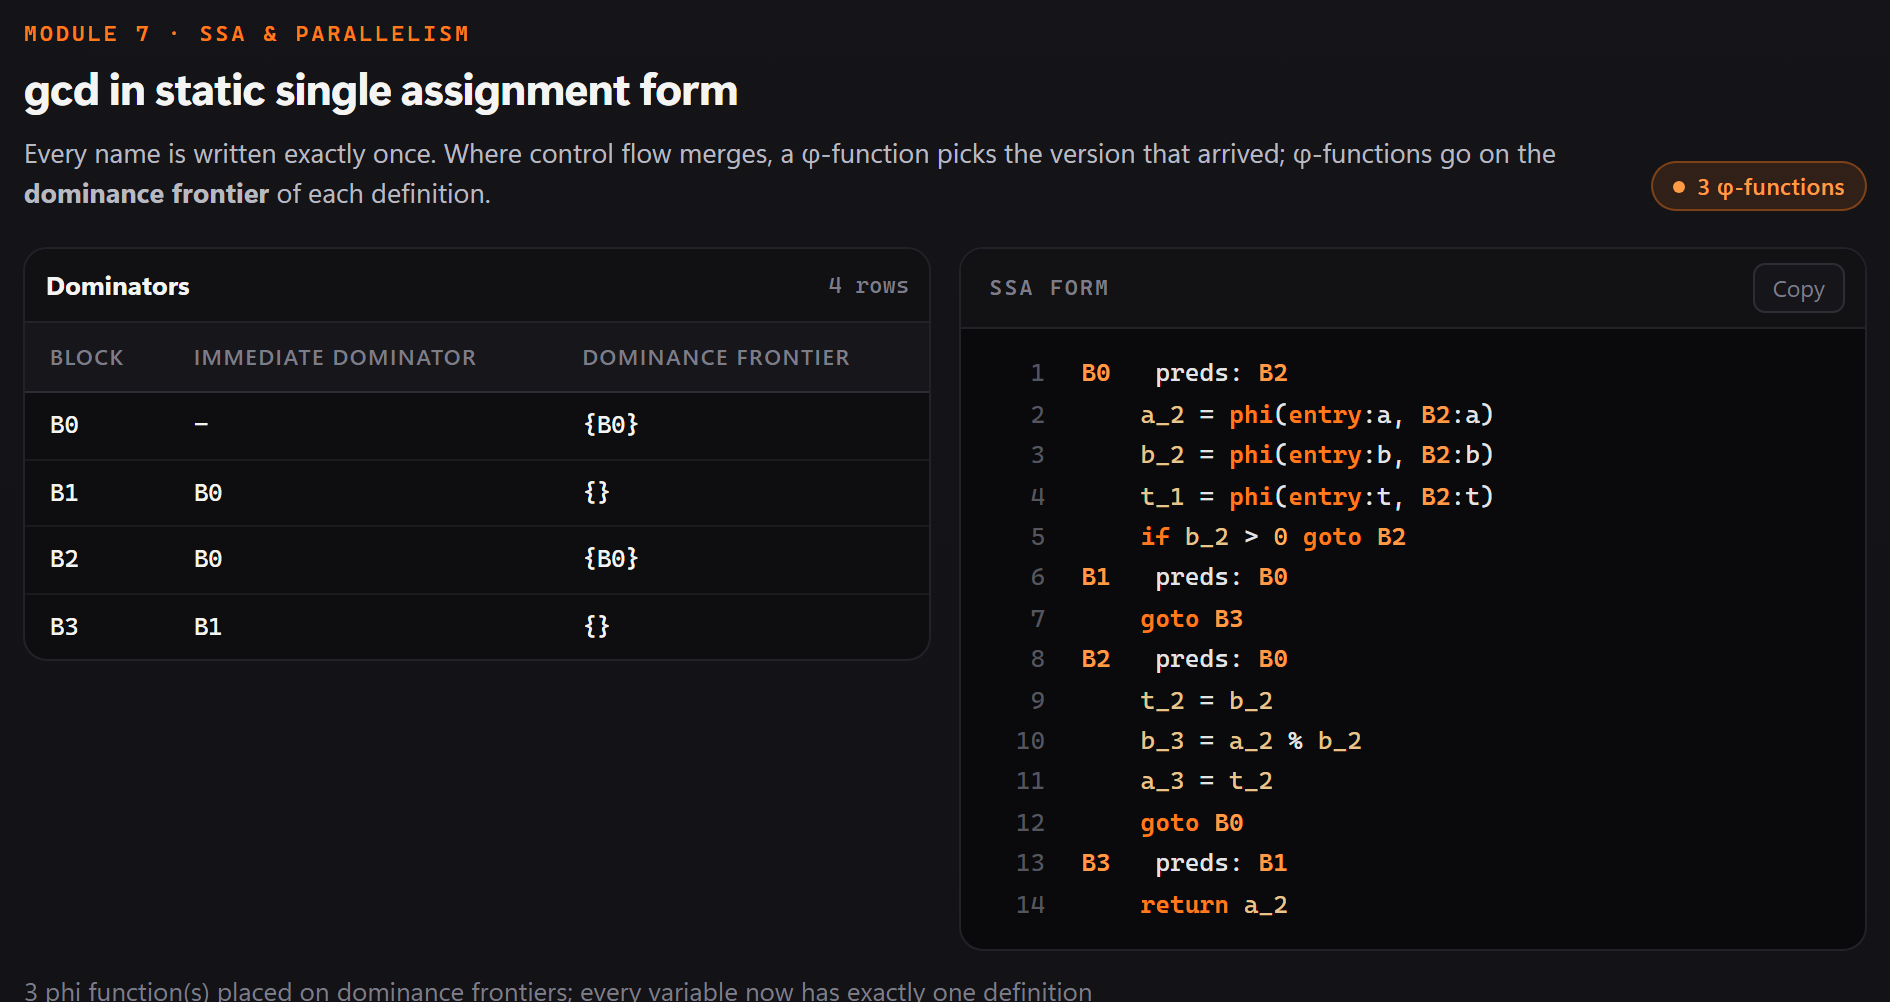
\includegraphics[width=0.74\textwidth]{figures/view-ssa.png}
\caption{SSA view of \code{gcd}. Its loop header is also the entry block, so \code{B0} is in its own dominance frontier and in that of \code{B2}. The $\phi$-functions merge each variable's value on entry with the value from the back edge, and the condition and \code{return} read the $\phi$ results.}
\label{fig:ssa}
\end{figure*}

\begin{figure}[!t]
\centering
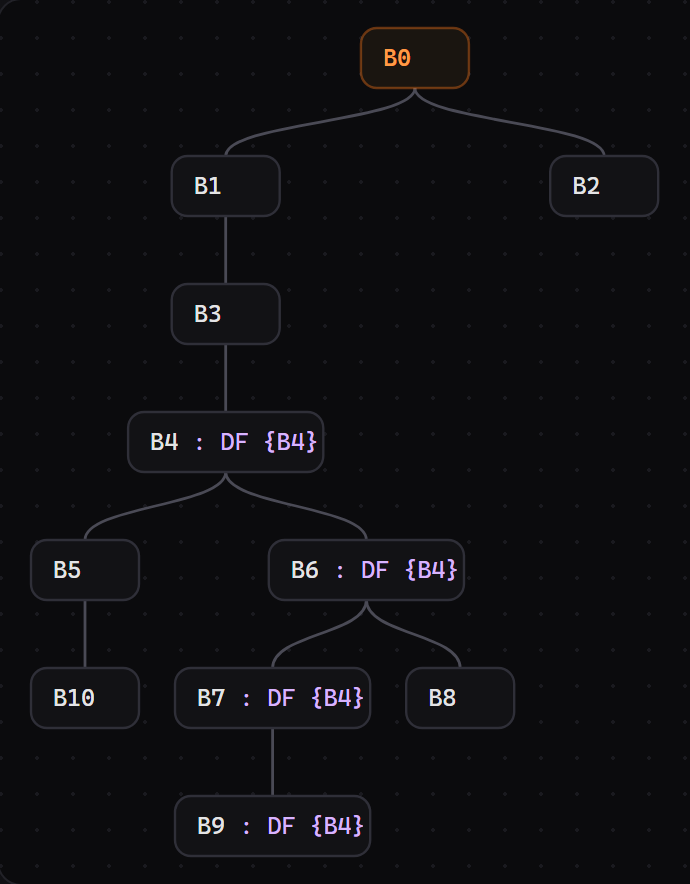
\includegraphics[width=0.62\columnwidth]{figures/dom-tree.png}
\caption{The dominator tree of \code{isprime} in \code{04\_primes.nova}. The loop header \code{B4} dominates the whole loop and is in its own dominance frontier; the blocks inside the loop that can reach the header again (\code{B6}, \code{B7}, \code{B9}) have \code{B4} in their frontier too, which is why the $\phi$-functions for \code{d} and the temporaries are placed in \code{B4}.}
\label{fig:domtree}
\end{figure}

\begin{figure*}[!t]
\centering
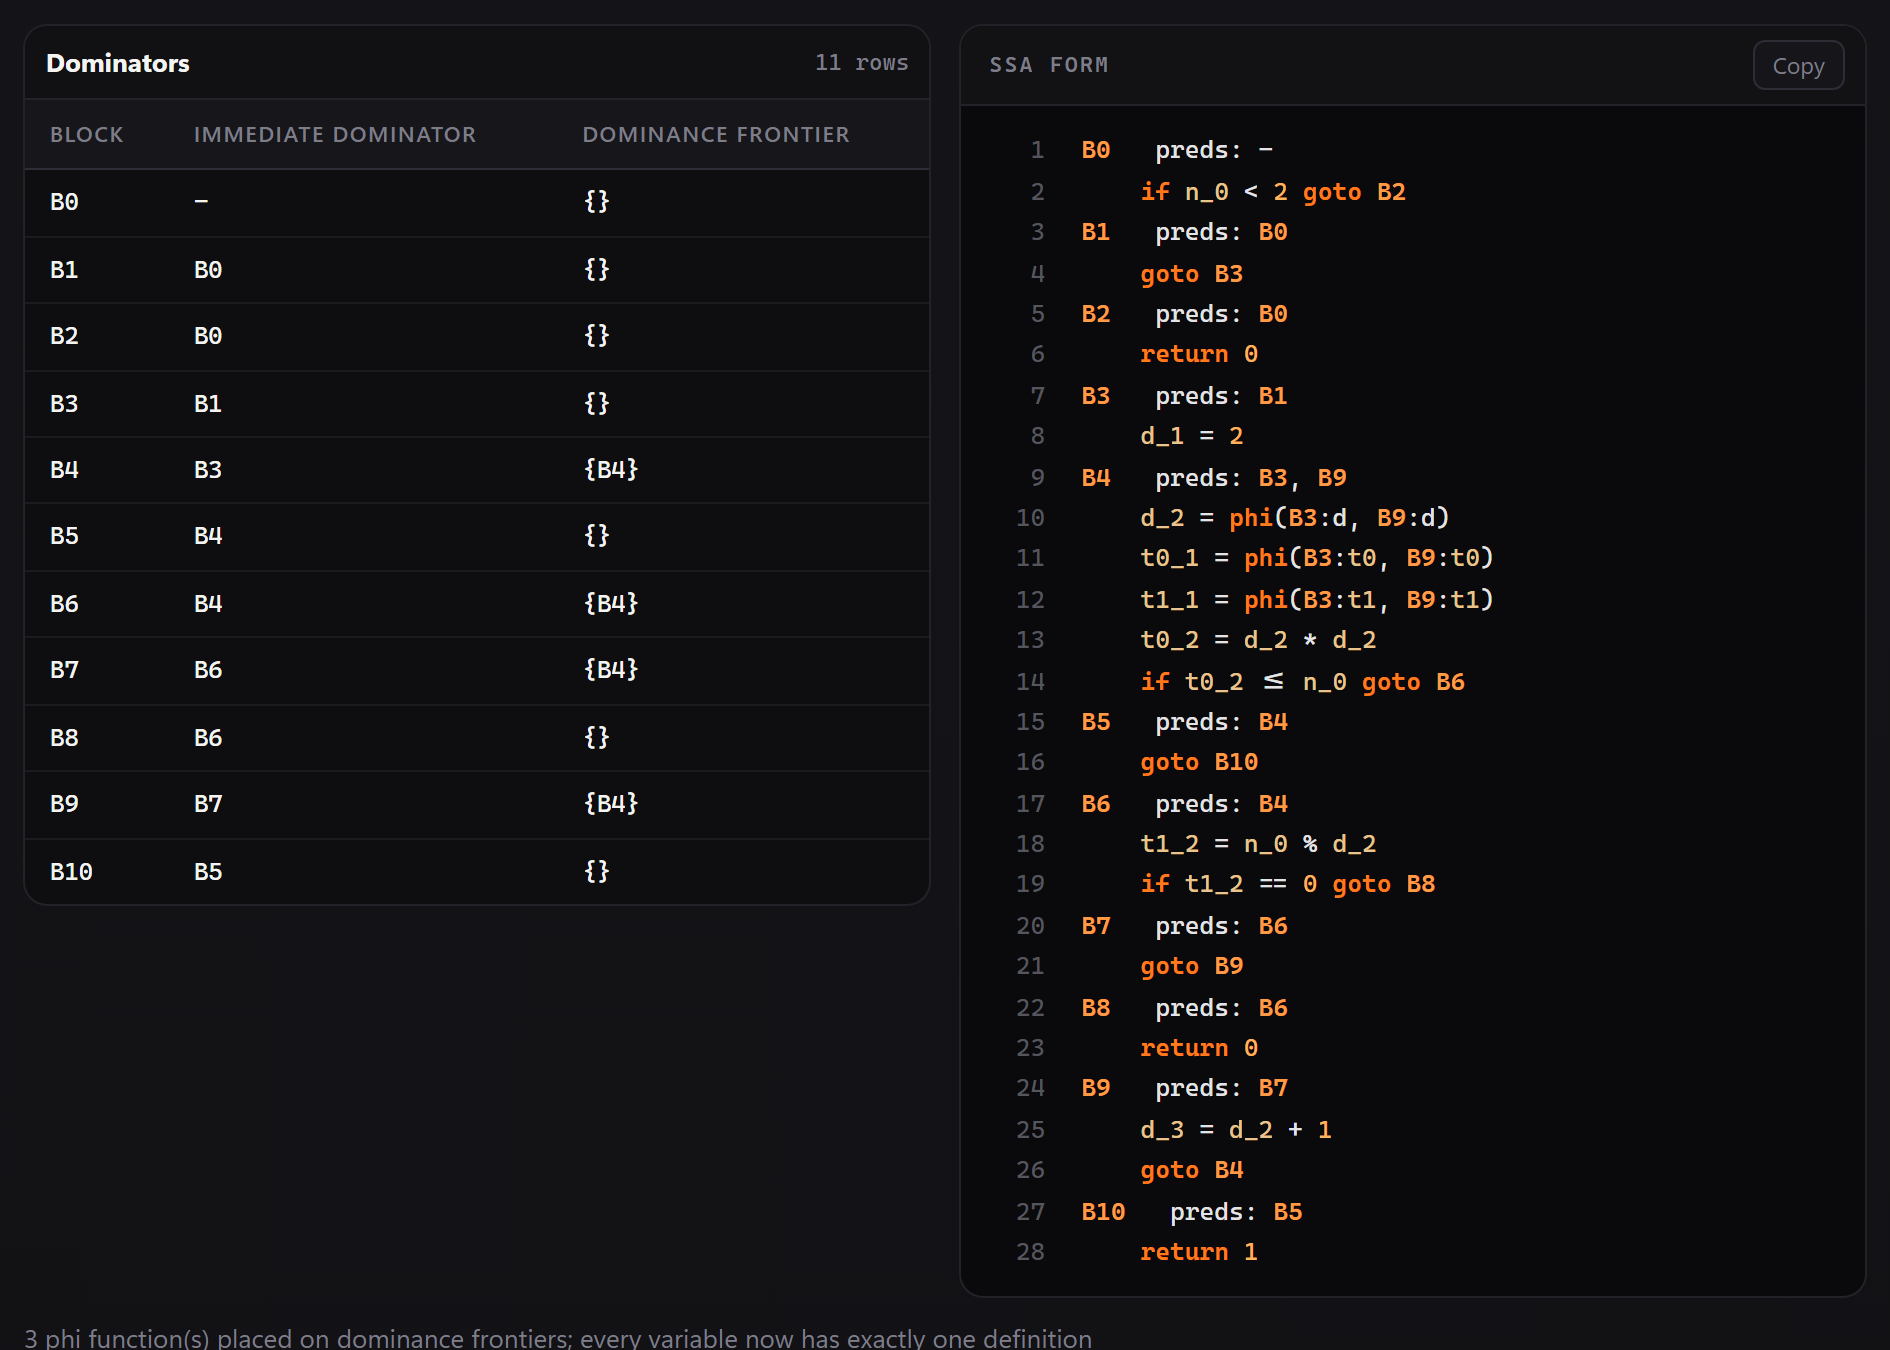
\includegraphics[width=0.8\textwidth]{figures/ssa-primes.png}
\caption{SSA view of \code{isprime} in \code{04\_primes.nova}: the dominator table with each block's immediate dominator and dominance frontier (left), and the renamed code (right). The three $\phi$-functions in \code{B4} merge the values of \code{d}, \code{t0} and \code{t1} arriving from \code{B3} (first iteration) and \code{B9} (back edge).}
\label{fig:ssaprimes}
\end{figure*}

\begin{figure}[!t]
\centering
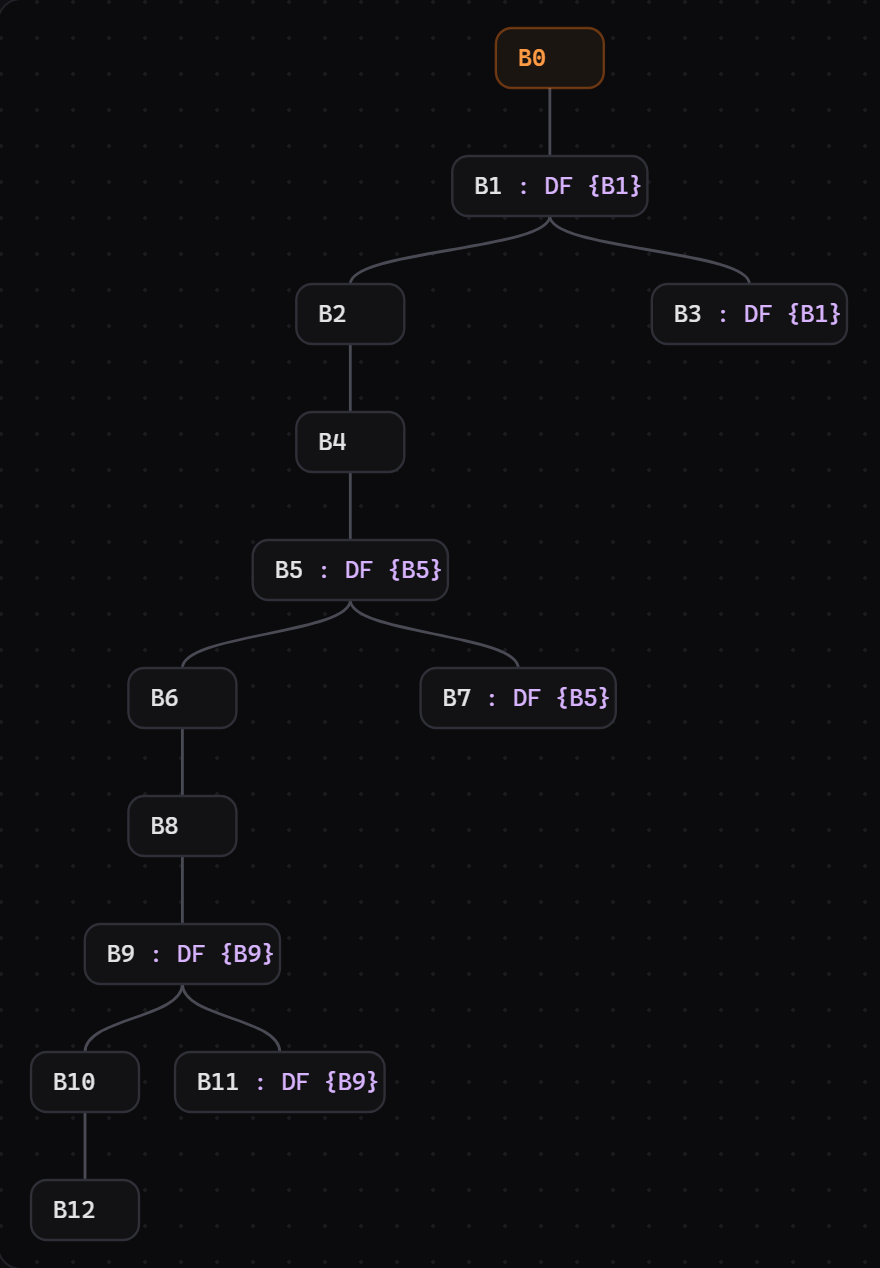
\includegraphics[width=0.62\columnwidth]{figures/dom-parallel.png}
\caption{The dominator tree of \code{main} in \code{06\_parallel.nova}. The three loops are dominated in sequence; each loop header (\code{B1}, \code{B5}, \code{B9}) is in its own dominance frontier and in that of its loop body (\code{B3}, \code{B7}, \code{B11}), which is where the $\phi$-functions of each loop are placed.}
\label{fig:domparallel}
\end{figure}

\begin{figure}[!t]
\centering
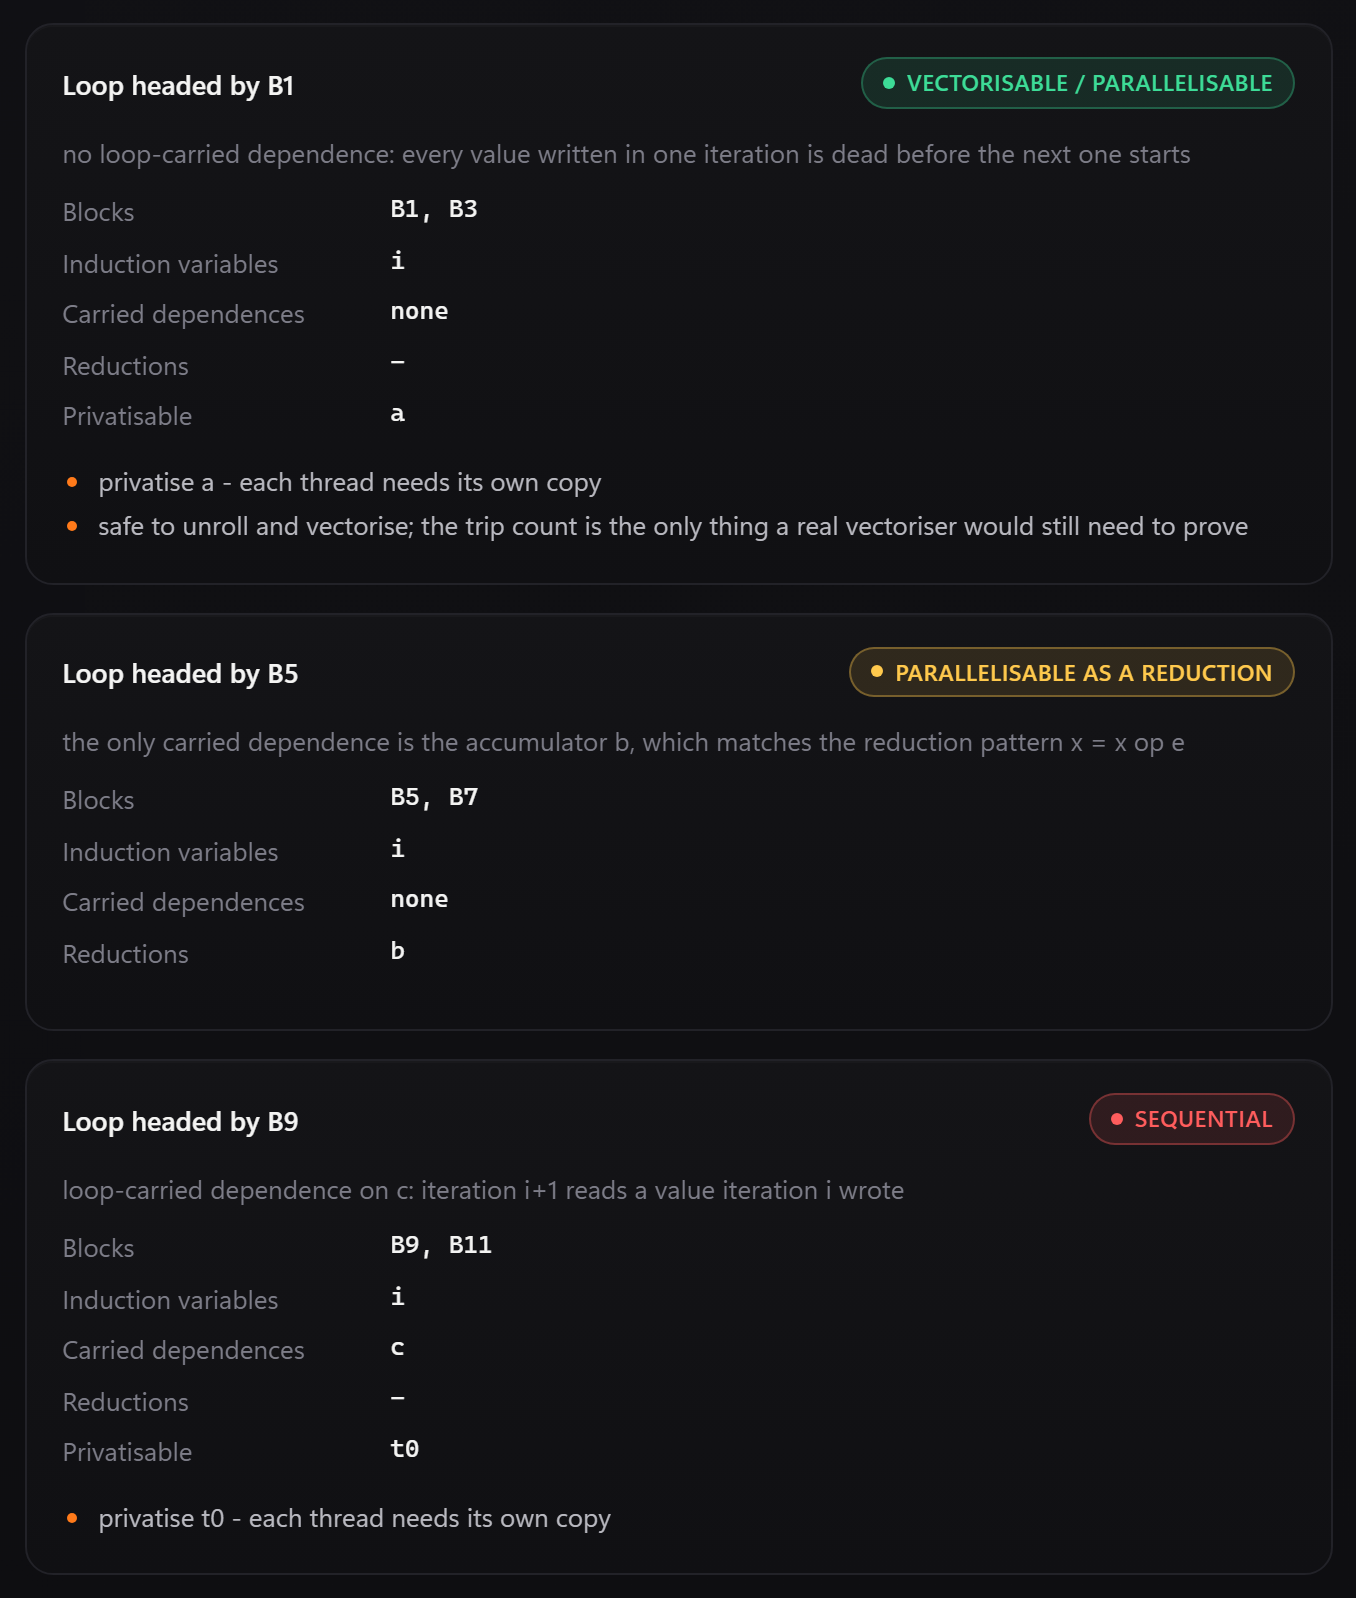
\includegraphics[width=0.94\columnwidth]{figures/view-loops.png}
\caption{Loop dependence analysis of \code{06\_parallel.nova}. Three loops that look alike are classified as vectorisable (no carried dependence; \code{a} is privatisable), parallelisable as a reduction (accumulator \code{b}) and sequential (iteration $i+1$ reads the value of \code{c} written by iteration $i$).}
\label{fig:loops}
\end{figure}

\begin{figure}[!t]
\centering
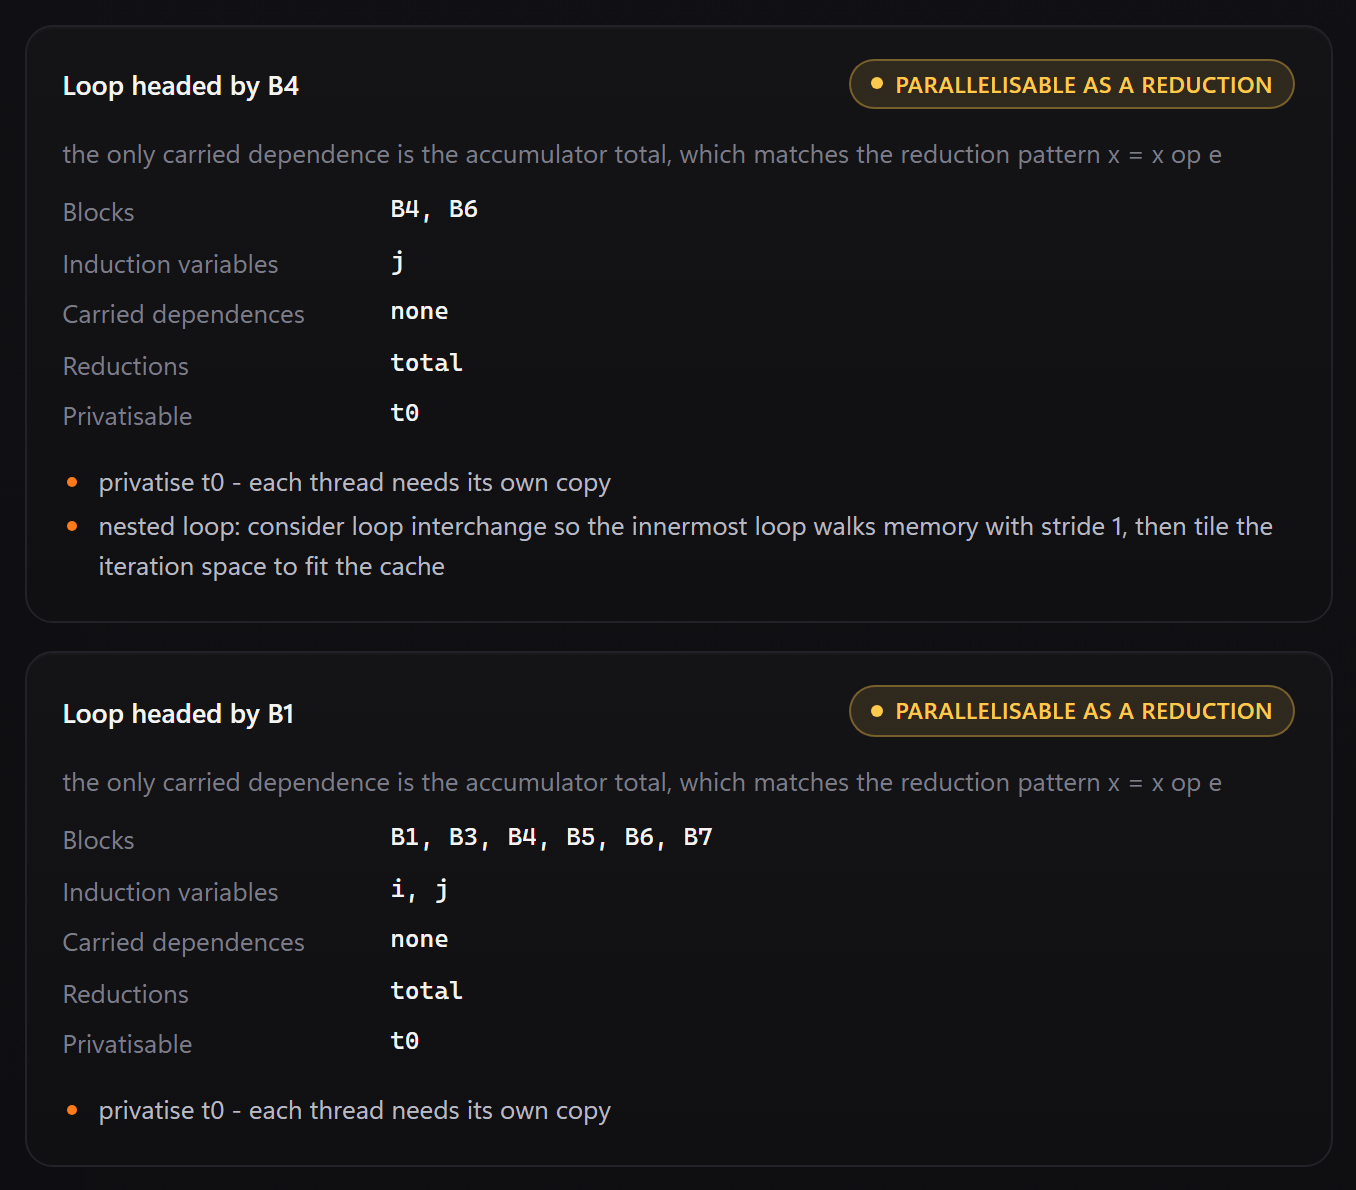
\includegraphics[width=0.94\columnwidth]{figures/nested-loops.png}
\caption{The nested loop pair of \code{09\_nested\_loops.nova}. Both loops are reductions on \code{total}; the inner loop additionally receives the locality advice---interchange so that the innermost loop walks memory with stride one, then tile---that a nested loop earns.}
\label{fig:nested}
\end{figure}

\subsection{Bytecode, Verification and Sandboxed Execution}
\label{sec:verify}
\emph{Bytecode.} The second back-end emits a JVM-like stack bytecode of 24 opcodes:
\begin{itemize}
\item constants, \code{LOAD} and \code{STORE};
\item arithmetic and \code{NEG};
\item \code{DUP} and \code{POP};
\item six conditional branches, \code{GOTO} and \code{SWITCH};
\item \code{PRINT}, \code{CALL}, \code{RETURN} and \code{HALT}.
\end{itemize}
A peephole pass~\cite{mckeeman1965} rewrites \code{STORE x; LOAD x} as \code{DUP; STORE x}, removes jumps to the next instruction and cancels double negation (Figs.~\ref{fig:bytecode} and~\ref{fig:peephole}).

\emph{Verification.} Before anything runs, the verifier performs abstract interpretation~\cite{cousot1977} over each function's bytecode (Algorithm~\ref{alg:verify}). The abstract state at instruction $i$ is $\sigma_i = (\tau, D)$, where $\tau$ is a stack of abstract types drawn from $\{\mathit{int},\mathit{str},\mathit{any}\}$ and $D$ is the set of definitely initialised local slots. At a merge point the stack depths must be equal; the types are joined pointwise (equal types are kept, unequal ones become $\mathit{any}$), and the sets $D$ are intersected. Because depths are fixed at merges, types only move towards $\mathit{any}$ and $D$ only shrinks, the iteration terminates. The verifier proves six properties: (P1)~a consistent operand-stack depth at every merge, (P2)~type safety of every instruction, (P3)~every branch target is inside the code, (P4)~definite assignment, (P5)~no \code{LOAD}/\code{STORE} outside the activation record, and (P6)~no unreachable instructions (reported as a warning). It also records the proved stack depth at every instruction, which the studio serves with the verification report.

\begin{algorithm}[!t]
\caption{Bytecode verification by abstract interpretation}
\label{alg:verify}
\begin{algorithmic}[1]
\REQUIRE function code $c_0..c_{n-1}$ with $p$ parameters and $s$ slots
\ENSURE a verdict for each of the properties P1--P6
\STATE $\sigma_0 \gets (\langle\,\rangle, \{0,\dots,p-1\})$;\ \ $W \gets \{0\}$
\WHILE{$W \neq \emptyset$}
  \STATE remove some $i$ from $W$;\ \ $(\tau, D) \gets \sigma_i$
  \STATE $(\tau', D') \gets \mathit{transfer}(c_i, \tau, D)$ \COMMENT{P2, P4, P5}
  \FORALL{$j \in \mathit{succ}(i)$}
    \IF{$j \notin [0, n)$}
      \STATE report a branch outside the code \COMMENT{P3}
    \ELSIF{$\sigma_j$ is undefined}
      \STATE $\sigma_j \gets (\tau', D')$;\ \ $W \gets W \cup \{j\}$
    \ELSIF{$|\tau_j| \neq |\tau'|$}
      \STATE report inconsistent stack depth \COMMENT{P1}
    \ELSE
      \STATE $\sigma'' \gets (\tau_j \sqcup \tau',\ D_j \cap D')$
      \IF{$\sigma'' \neq \sigma_j$}
        \STATE $\sigma_j \gets \sigma''$;\ \ $W \gets W \cup \{j\}$
      \ENDIF
    \ENDIF
  \ENDFOR
\ENDWHILE
\STATE report every instruction never reached \COMMENT{P6}
\end{algorithmic}
\end{algorithm}

\emph{Sandboxed execution.} The VM refuses unverified code. A call pushes a frame holding the callee's locals, its operand stack, the return address and a control link to the caller's frame. Execution runs under hard limits of 2,000,000 instructions, 256 frames and 1,024 operand-stack entries, so a non-terminating or runaway program is reported as a policy violation instead of hanging the tool. The VM records the first 400 steps as a trace---each step with its function, program counter, instruction, operand stack, call depth and the locals of the current frame---and keeps a snapshot of the activation-record stack at its deepest (Figs.~\ref{fig:verifier} and~\ref{fig:execution}). A hostile-bytecode suite of eight hand-written programs, discussed in Section~\ref{sec:res-security}, exercises the verifier and the sandbox together.

\emph{The VM stepper.} The studio replays the trace as a stepper (Fig.~\ref{fig:stepper}): the bytecode of the current function with the program counter highlighted, the operand stack top first, the locals of the current frame by name, the call depth against the deepest reached, and the output produced so far. It steps, scrubs and autoplays at 260\,ms per instruction, and answers the same keys as the parse player. Fig.~\ref{fig:stepperstrings} shows the stepper at the last instruction of \code{10\_strings.nova}, after the \code{SWITCH} of the \code{case} statement has taken its default branch: all four lines of output have appeared, and the locals hold \code{count = 3} and \code{ok = 1}, the run-time representation of \code{true}.

\emph{LLVM IR.} A third back-end prints textual LLVM IR in the style of \code{clang -O0}: every variable becomes an \code{alloca}, and reads and writes become \code{load} and \code{store} (Fig.~\ref{fig:llvm}). LLVM's \code{mem2reg} pass would produce the same SSA form that Nova builds itself. The output needs no LLVM installation, but anyone who has \code{clang} can compile it to native code.

\begin{figure}[!t]
\centering
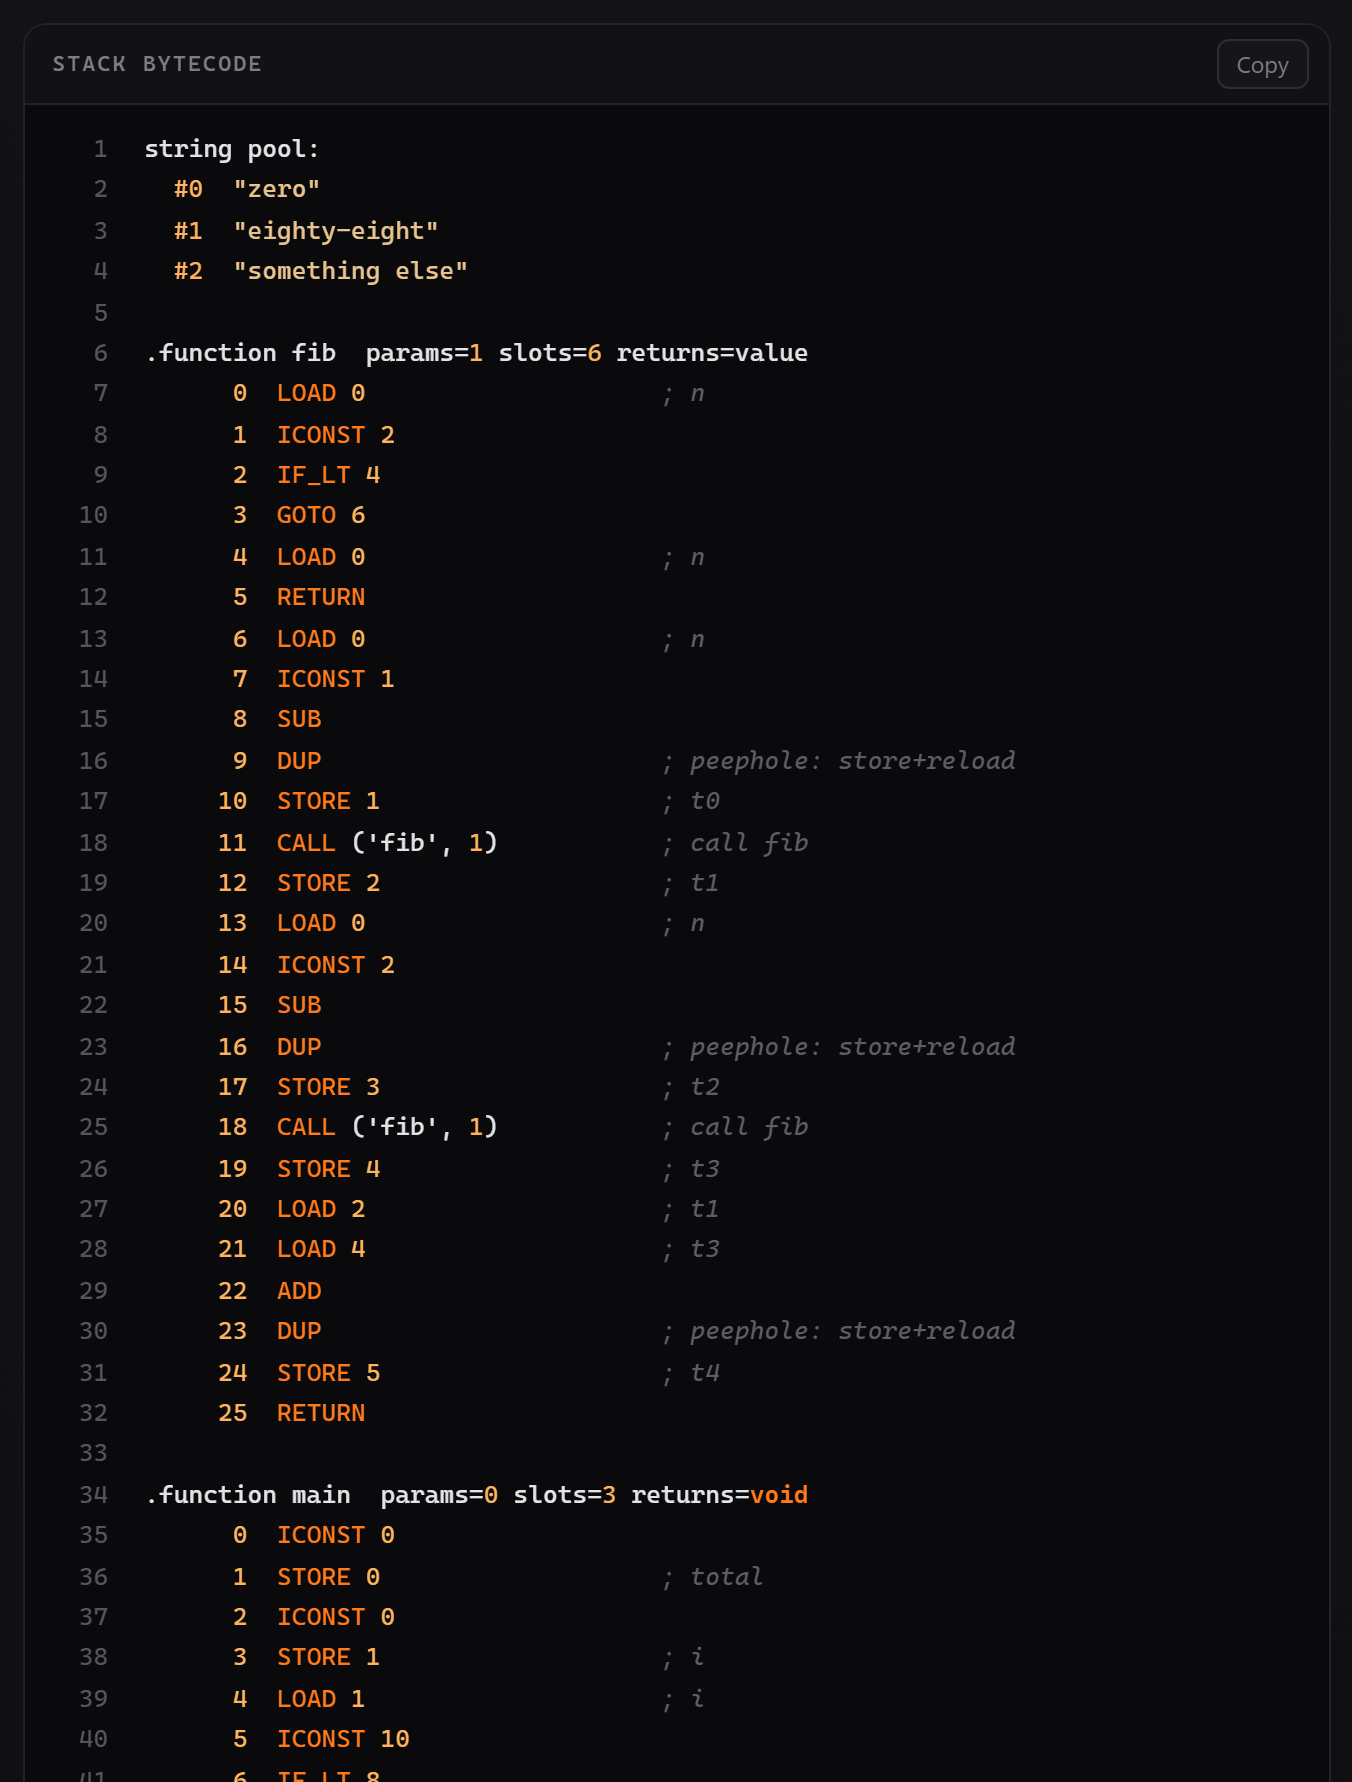
\includegraphics[width=\columnwidth]{figures/bytecode.png}
\caption{The stack bytecode of the Fibonacci program: the string pool, then \code{fib} with its parameter and slot counts. The verifier's maximum stack depth of 2 is visible in the code---no instruction ever needs more than two operands.}
\label{fig:bytecode}
\end{figure}

\begin{figure}[!t]
\centering
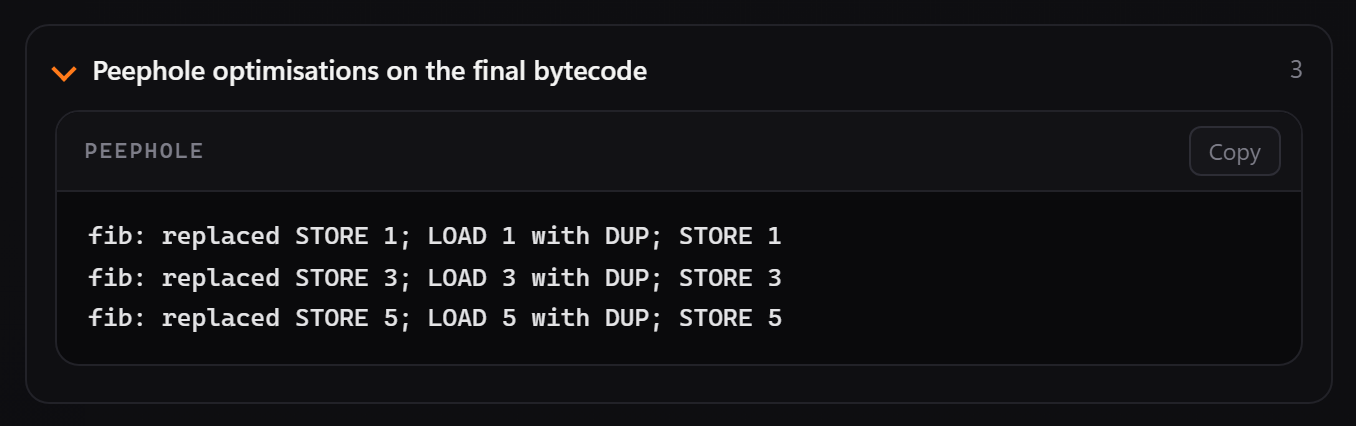
\includegraphics[width=\columnwidth]{figures/peephole.png}
\caption{Peephole optimisations applied to the final bytecode of the Fibonacci program: three \code{STORE x; LOAD x} pairs rewritten as \code{DUP; STORE x}.}
\label{fig:peephole}
\end{figure}

\begin{figure}[!t]
\centering
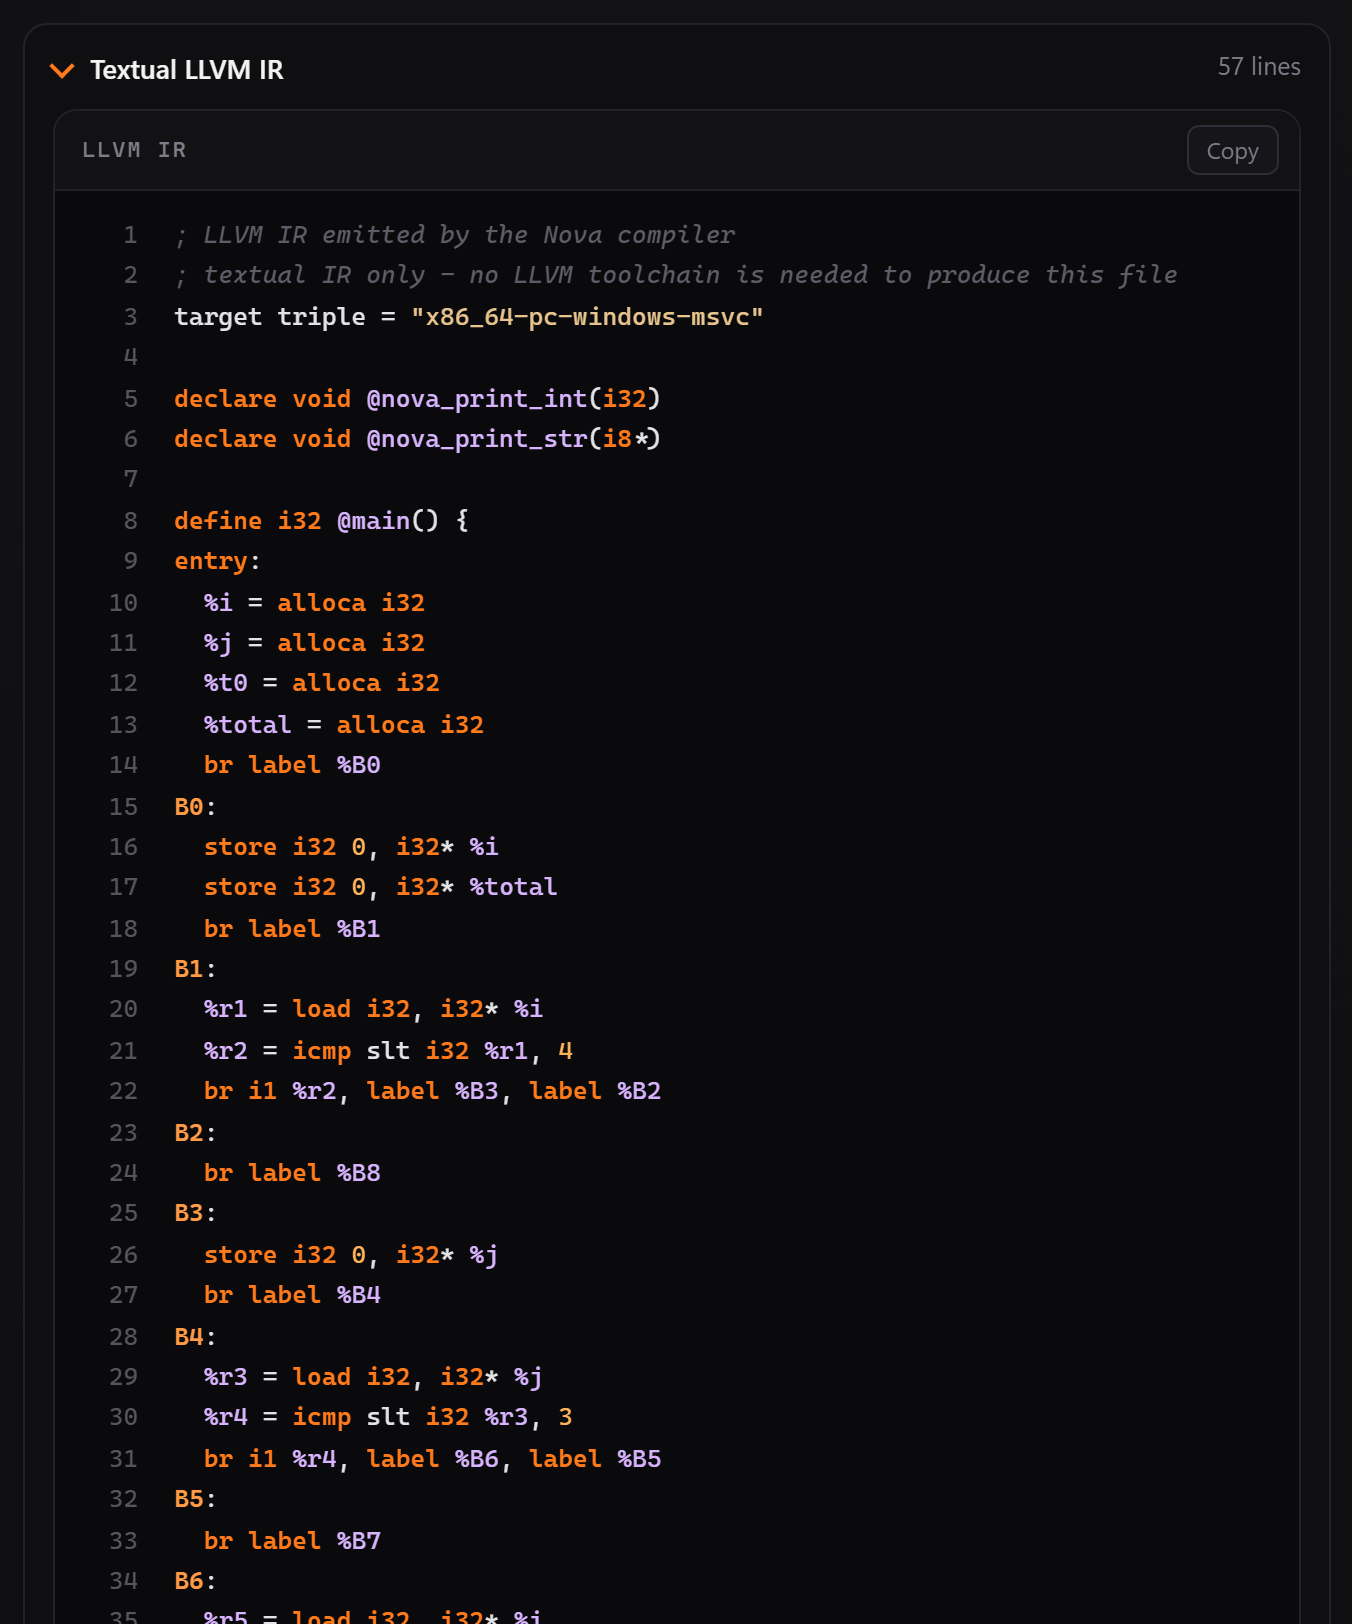
\includegraphics[width=\columnwidth]{figures/llvm-ir.png}
\caption{The textual LLVM IR for the Fibonacci program: every Nova variable is an \code{alloca} slot, every read a \code{load} and every write a \code{store}, exactly as \code{clang -O0} would emit it.}
\label{fig:llvm}
\end{figure}

\begin{figure}[!t]
\centering
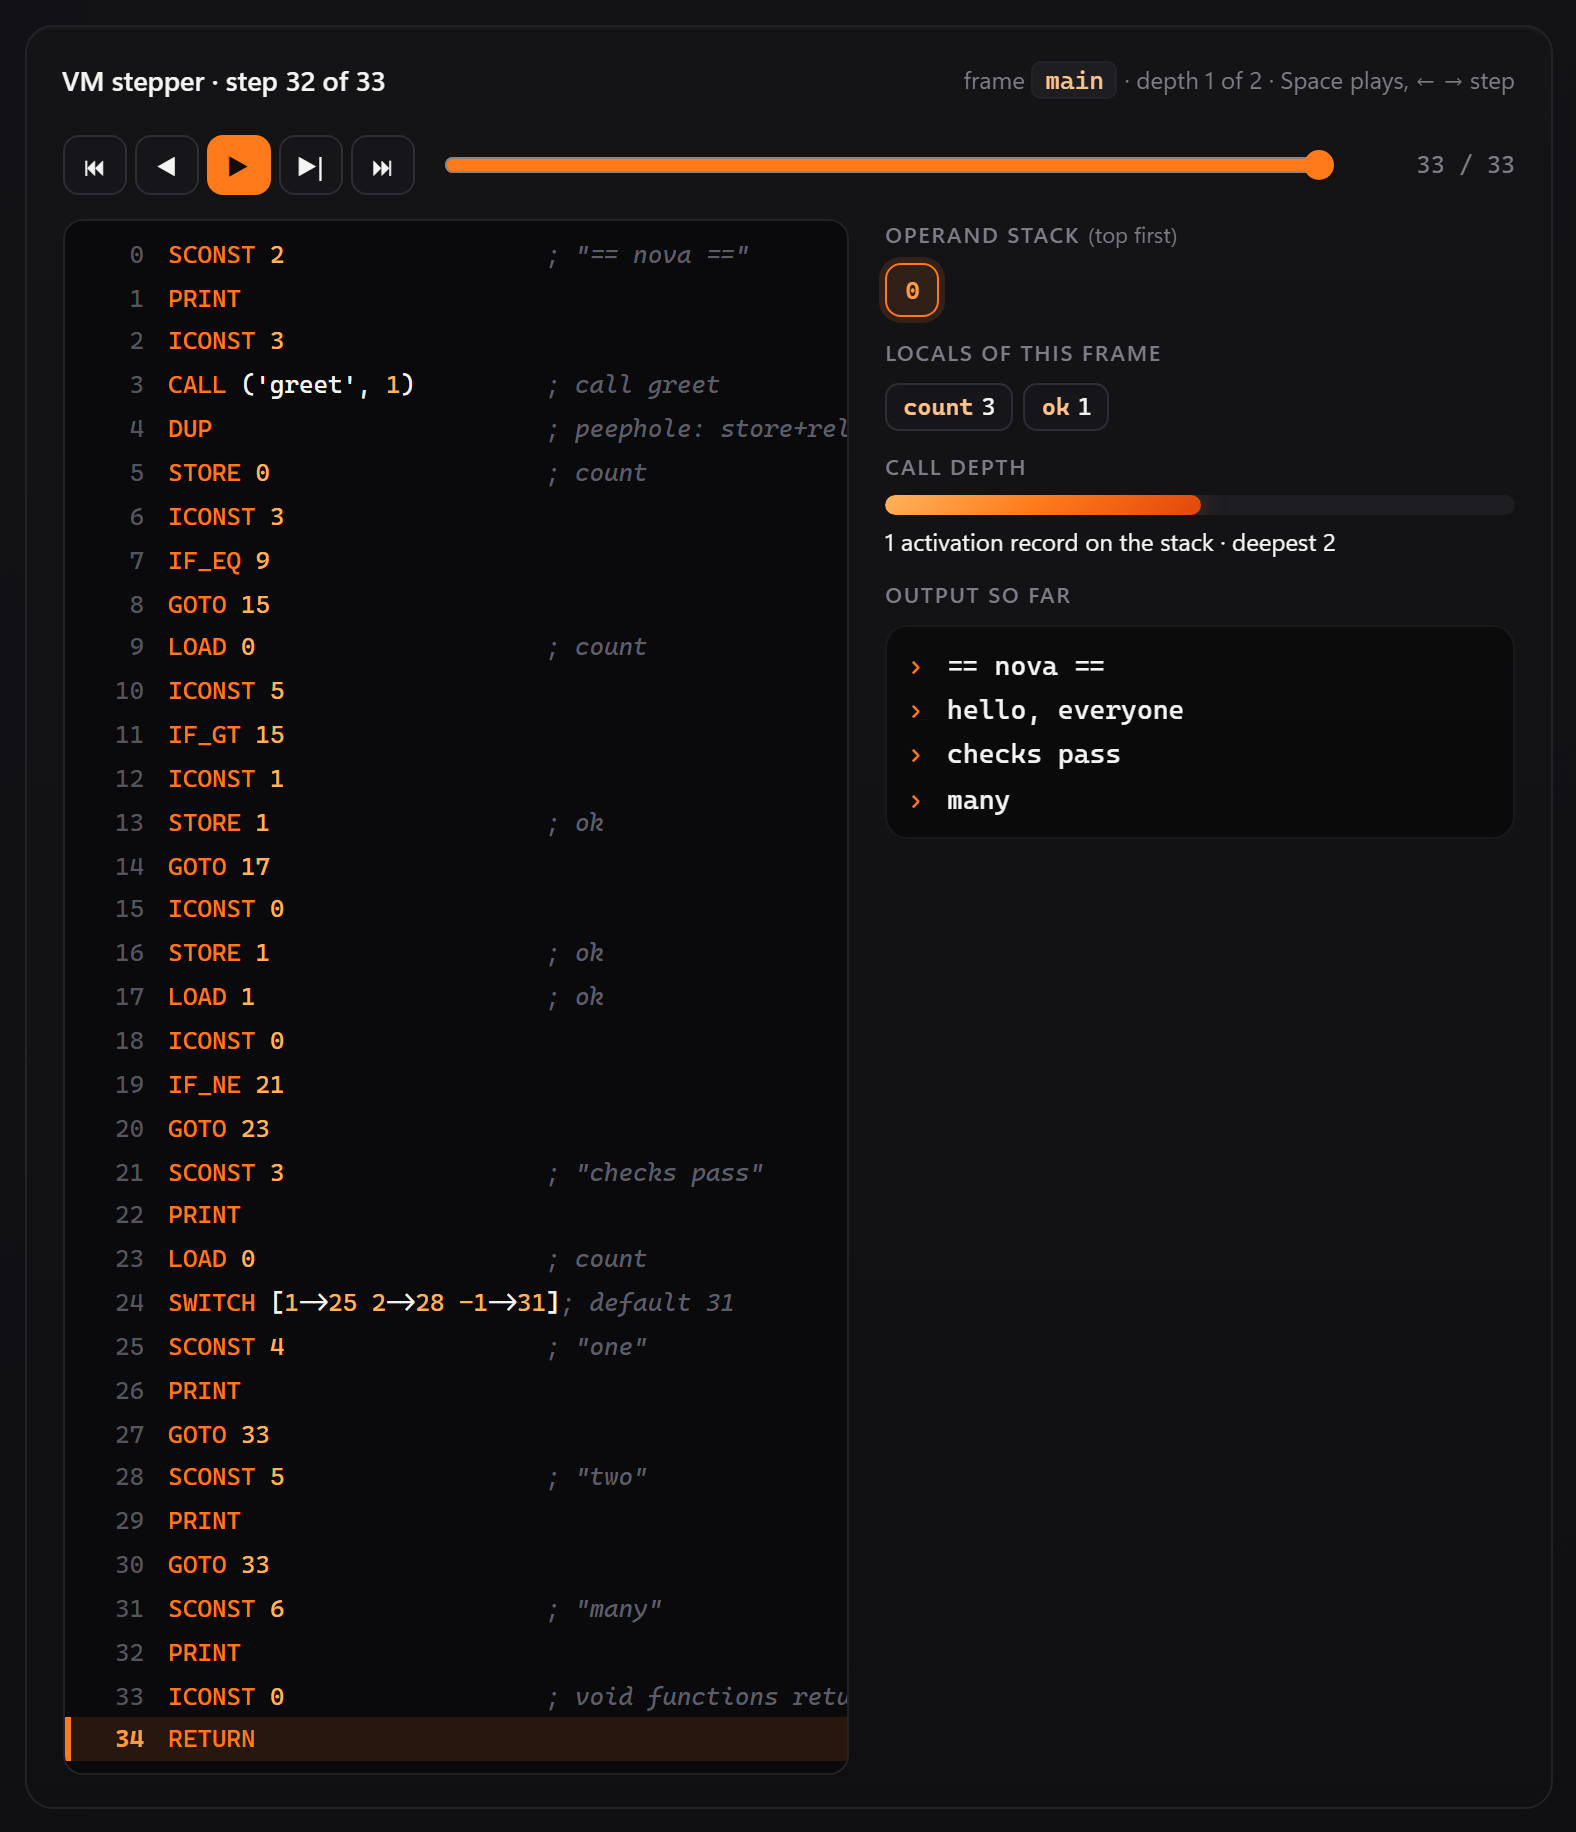
\includegraphics[width=\columnwidth]{figures/vm-stepper-strings.png}
\caption{The VM stepper at the final instruction of \code{10\_strings.nova}. The \code{SWITCH} at instruction 24 compiles the \code{case} statement; its default target 31 printed \code{many}. All four output lines are visible, and the frame's locals are \code{count = 3} and \code{ok = 1}.}
\label{fig:stepperstrings}
\end{figure}

\subsection{Nova Studio}
\label{sec:studio}
\emph{Architecture.} Nova Studio is a local web application served by a standard-library \code{ThreadingHTTPServer}~\cite{pythonhttp}. A JSON view module mirrors the HTML report: it renders a \code{CompileResult} as plain dictionaries and lists (Table~\ref{tab:json}), and it caps long lists at 2,500 rows while recording their true lengths. The API is summarised in Table~\ref{tab:api}. The client is a single page written in plain JavaScript (1,846 lines) and CSS (837 lines), with no frameworks and no build step; it is served with a content hash in its URLs so that a browser never runs a stale copy.

\begin{table}[!t]
\caption{The Compile JSON Document}
\label{tab:json}
\centering
\footnotesize
\setlength{\tabcolsep}{4pt}
\begin{tabular}{@{}l L{5.1cm}@{}}
\toprule
Key & Contents \\
\midrule
\code{diagnostics} & phase, line, column, message, hint, severity \\
\code{lexical} & DFA statistics, tokens, followpos rows, DFA rows, and per token the DFA path and read-ahead \\
\code{syntax} & the three tables' sizes, the LALR(1) verdict and trace, the recursive-descent trace \\
\code{semantic} & symbol rows, attribute-flow rows, the annotated tree as text and as nested nodes \\
\code{functions[]} & per function: TAC, CFG before and after, pass records, DAG nodes, four data-flow solutions with rounds, frame layout, next-use rows, register decisions, target code, dominators, SSA blocks, loop reports \\
\code{bytecode} & listing, per-function code and slots, string pool, peephole notes, instruction counts \\
\code{verifier[]} & per function: six checks, errors, proved stack depth at every instruction \\
\code{run} & output, error, steps, frames, trace rows with locals, the other two back-ends, agreement \\
\makecell[l]{\code{summary}, \code{timings},\\ \code{metrics}} & the headline numbers and the measurement table \\
\bottomrule
\end{tabular}
\end{table}

\begin{table}[!t]
\caption{Nova Studio HTTP API}
\label{tab:api}
\centering
\footnotesize
\setlength{\tabcolsep}{4pt}
\begin{tabular}{@{}l L{4.85cm}@{}}
\toprule
Endpoint & Purpose \\
\midrule
\code{GET /api/health} & liveness, version and execution budgets \\
\code{GET /api/examples} & the eleven example programs \\
\code{GET /api/grammar} & grammar, FIRST/FOLLOW, LL(1) conflicts, ambiguity demonstration, DFA accepting states, the LALR(1) automaton and its ACTION/GOTO table (computed once) \\
\code{POST /api/compile} & \code{\{source, optimise, mode\}} $\to$ every phase as JSON \\
\code{POST /api/report} & the self-contained HTML report as a download \\
\code{GET /api/attacks} & hostile bytecode against verifier and sandbox \\
\bottomrule
\end{tabular}
\end{table}

\emph{Live compilation.} The editor sends a compile request 360\,ms after the user stops typing. The client keeps only the latest request: a new one aborts the request in flight, and a monotonically increasing sequence number discards stale responses. The server serialises compilations with a lock and builds the LR tables at start-up, before the first request. While the user types, each of the three executions receives a budget of 250,000 instructions, so an unfinished loop cannot freeze the page. Pressing \emph{Run} (\code{Ctrl+Enter}) restores the normal 2,000,000, and the studio says which budget stopped a program.

\emph{Instruments.} Beyond the tables and code listings, the inspector contains the interactive instruments listed in Table~\ref{tab:instruments}, each of which has been shown in the preceding subsections. All of them are drawn in the browser from the JSON document: the trees and the dominator tree by the tidy layout, the flow graphs and DAGs by layered layouts, the timeline as a table of coloured runs, and the two players as state machines over the trace rows. The three drawings share one layout engine, and the two players share one controller, so adding an instrument is a matter of a view function.

\begin{table}[!t]
\caption{Interactive Instruments in the Inspector}
\label{tab:instruments}
\centering
\footnotesize
\setlength{\tabcolsep}{3.5pt}
\begin{tabular}{@{}l c L{3.1cm}@{}}
\toprule
Instrument & Mod. & What the learner can do \\
\midrule
Scanner trace & 1 & click a token; see its DFA path, edges and accepting states \\
Automaton browser & 2 & step through all 116 states; follow shift and GOTO links; page the table \\
Parse player & 2 & replay 297 actions with both stacks, the handle and the look-ahead tape \\
Syntax tree & 3 & switch between functions and statements; read synthesised types \\
Pass waterfall & 5 & see what each of the ten passes removed or added \\
Flow graph & 5 & toggle before/after; read loops from back edges \\
DAG & 5 & choose a block; see shared nodes and attached variables \\
Data-flow overlay & 5 & choose an analysis; read IN/OUT on the graph \\
Register timeline & 6 & see every value's stay in every register \\
Dominator tree & 7 & read immediate dominators and frontiers \\
VM stepper & 8/9 & step the machine; watch stack, locals, depth, output \\
Syllabus map & all & see each module's requirement, implementation and numbers \\
\bottomrule
\end{tabular}
\end{table}

\emph{Interface.} The interface comprises the following components:
\begin{itemize}
\item a syntax-highlighting editor whose gutter marks diagnostics;
\item the nine-stage pipeline rail;
\item an inspector with fourteen views and a per-function selector;
\item filterable tables;
\item a problems panel that jumps to the offending line (Fig.~\ref{fig:diagnostics});
\item a syllabus map that connects each module of the course to the views that demonstrate it, with the numbers of the current program (Fig.~\ref{fig:syllabus});
\item deep links of the form \code{\#tab=optimiser\&fn=main}, and \emph{share} links that carry the whole program in the URL, so that a particular program and view can be sent to another person;
\item downloads of the HTML report and of the compile JSON;
\item keyboard shortcuts (Fig.~\ref{fig:keys}), and a layout that adapts down to a 390-pixel-wide phone screen (Fig.~\ref{fig:mobile}).
\end{itemize}
The pipeline rail (Fig.~\ref{fig:rail}) is the studio's summary of a compilation: one card per stage with a tick, a cross or a dash for passed, failed and skipped, and the stage's cost. Live compilation is shown at work in Fig.~\ref{fig:liveerror}: a loop typed with two semantic errors---a string added to an integer and a misspelt variable---is reported 0.85\,ms later, the rail marks semantic analysis as failed and every later stage as skipped, and the gutter and the problems panel point at lines 3 and 5. Clicking a problem moves the caret to its position and flashes the line (Fig.~\ref{fig:editorproblems}). The overview's own panels---the per-phase timing and the comparison of the three back-ends---are shown at full size in Fig.~\ref{fig:panels}, and the metrics view ends with the phase timings and the buttons that export the compilation (Fig.~\ref{fig:metricstimings}).


\begin{figure*}[!t]
\centering
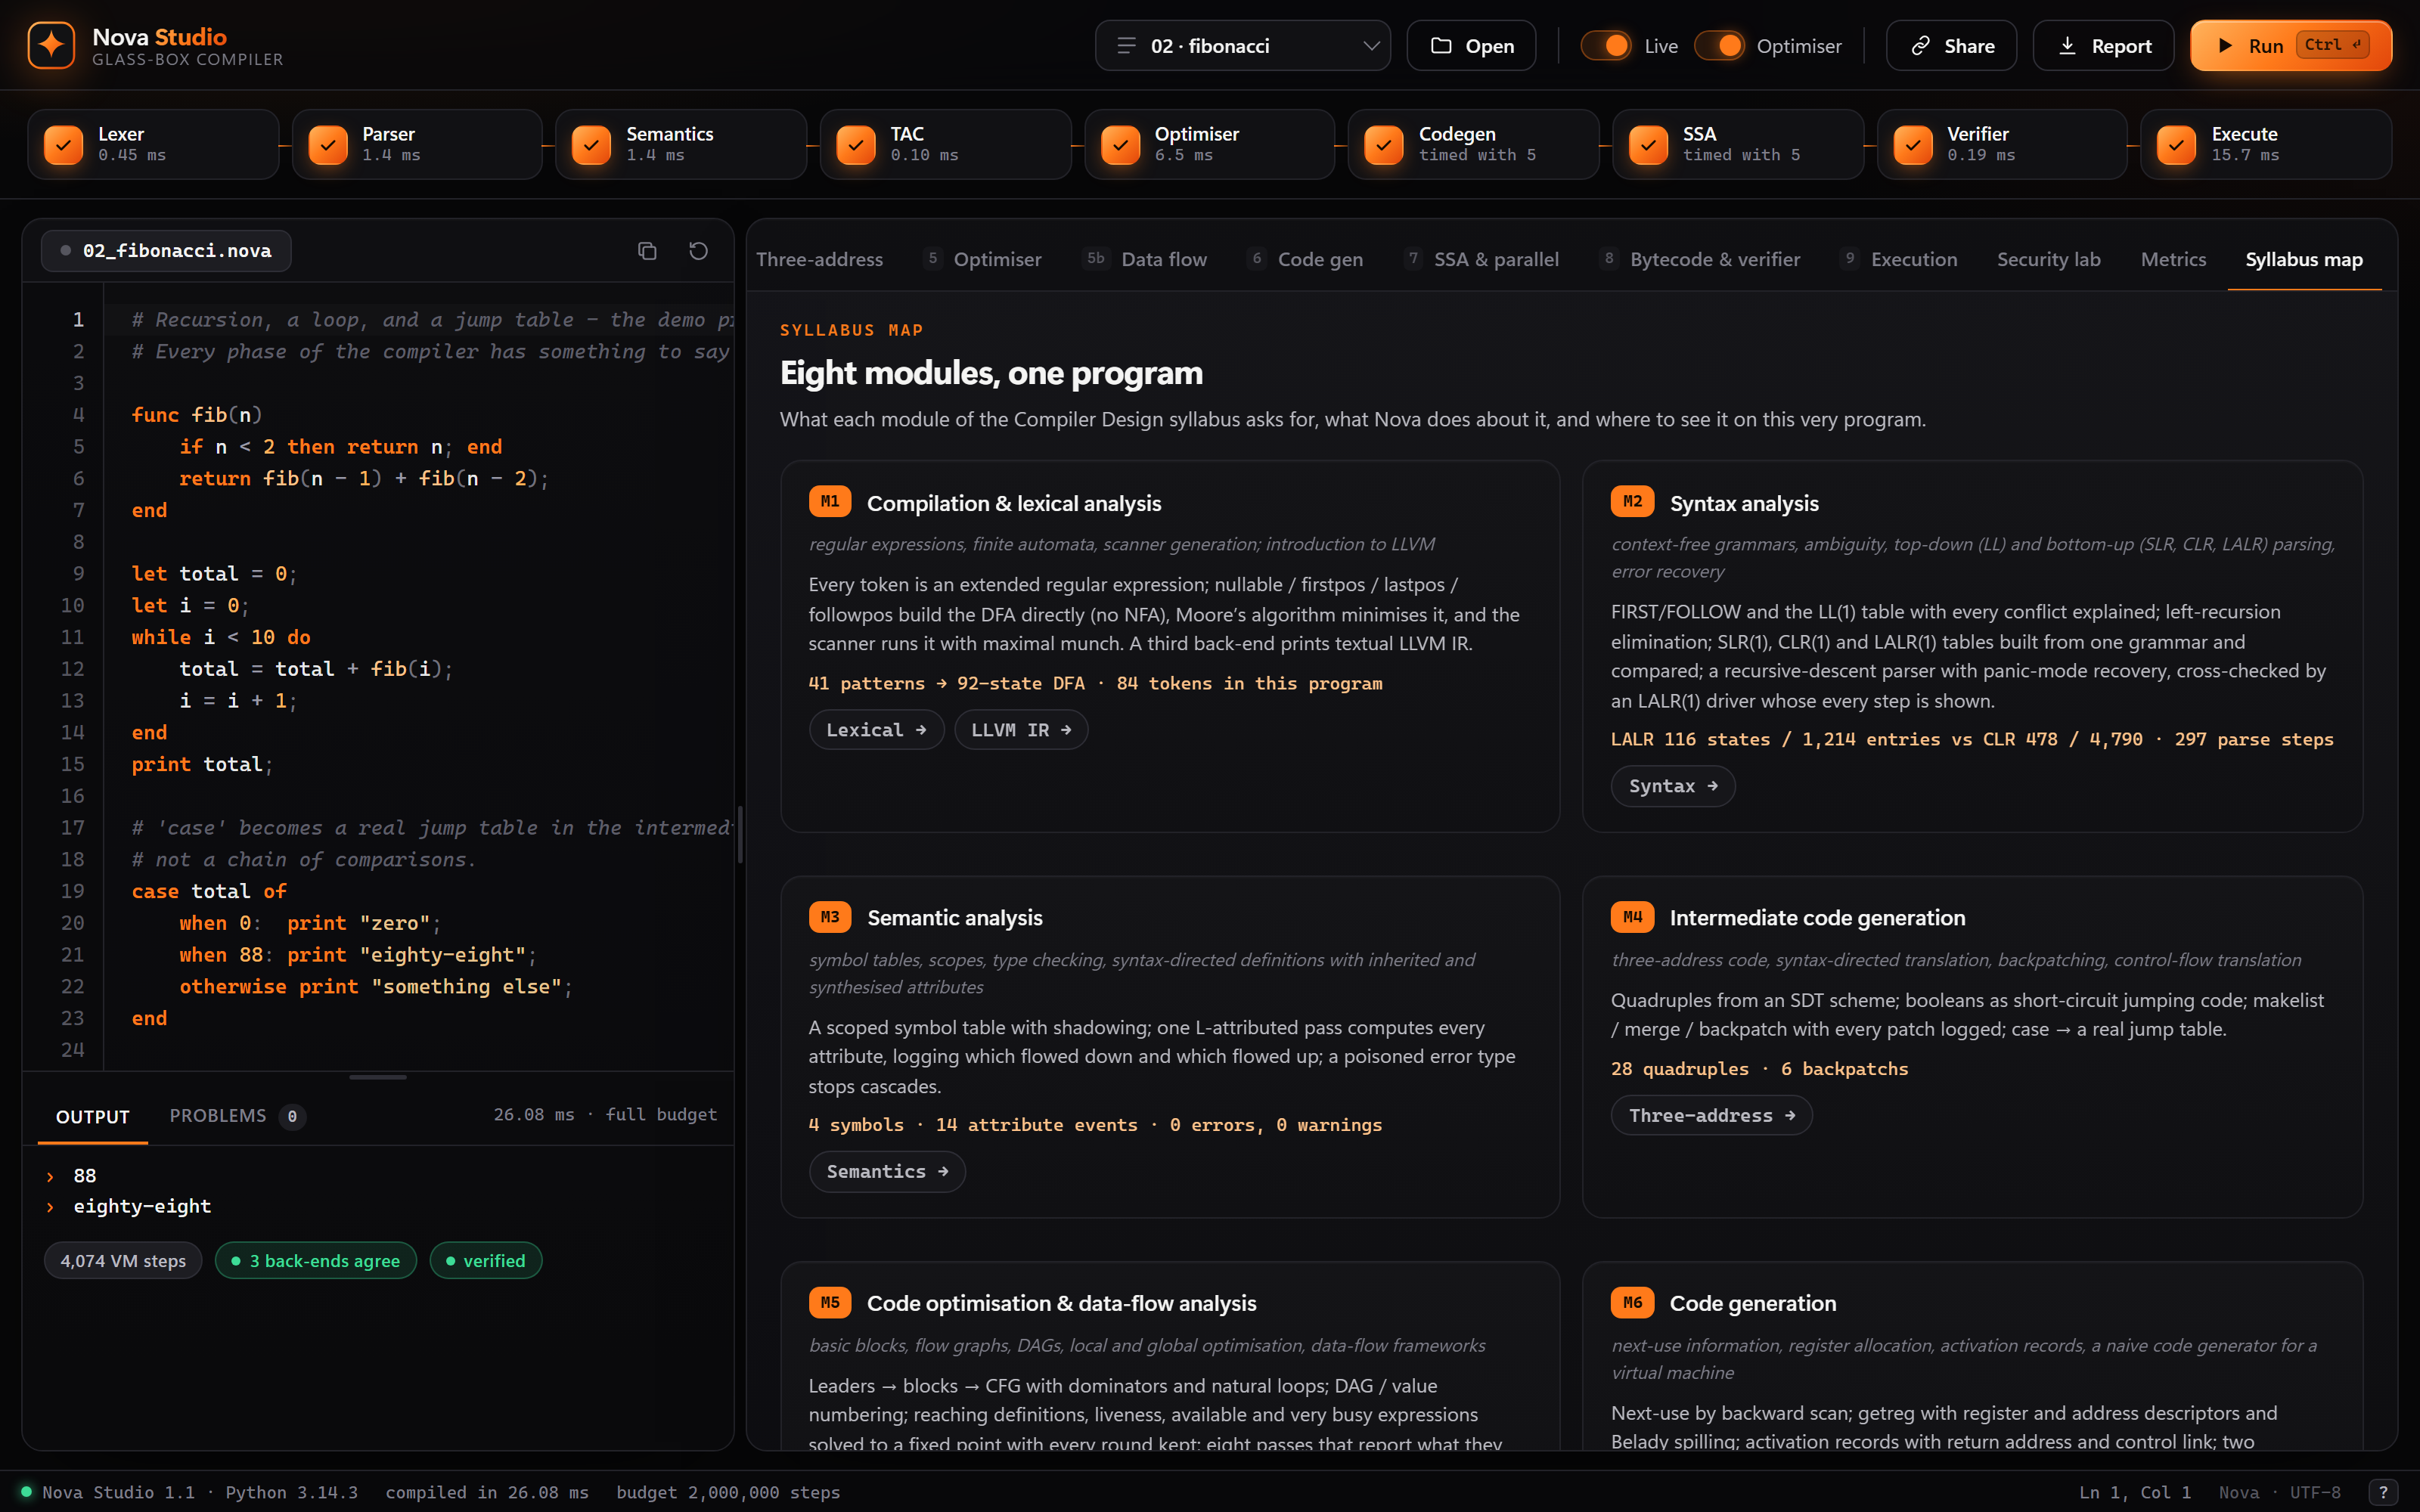
\includegraphics[width=\textwidth]{figures/syllabus.png}
\caption{The syllabus map. For each of the eight modules it states what the syllabus asks for, what Nova does about it, the measurements of the current program (here \code{02\_fibonacci.nova}) and links to the views that show it.}
\label{fig:syllabus}
\end{figure*}

\begin{figure}[!t]
\centering
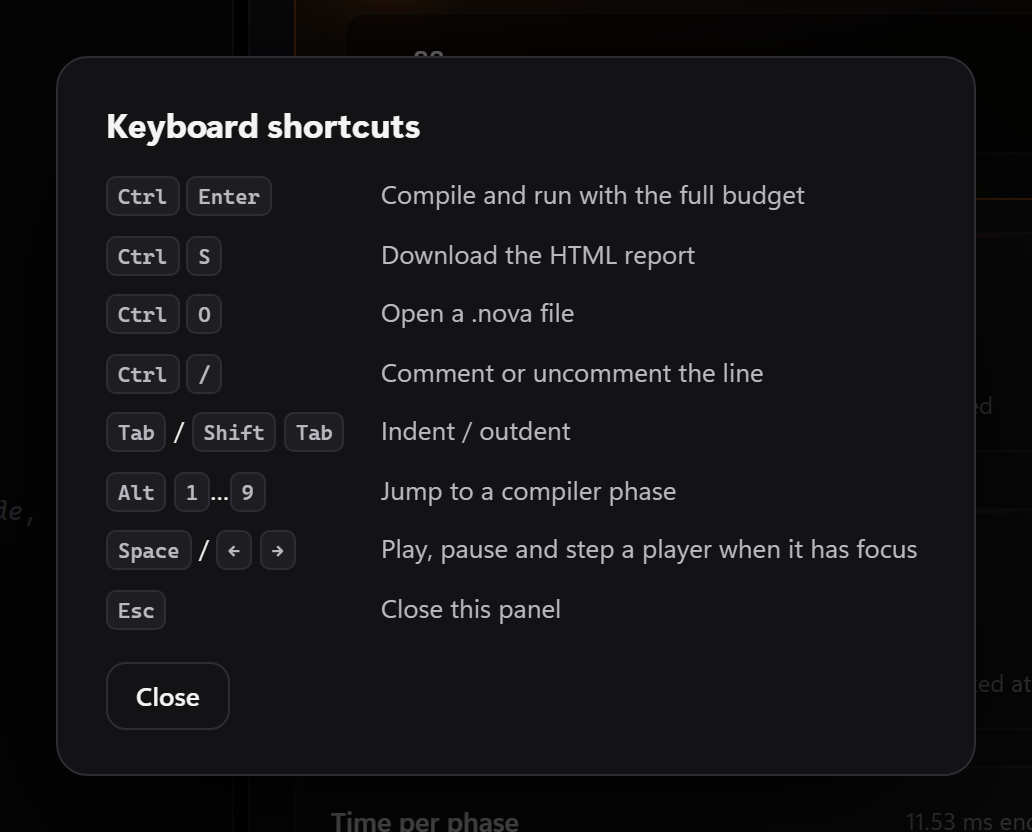
\includegraphics[width=0.82\columnwidth]{figures/keys-modal.png}
\caption{The keyboard-shortcut panel. \code{Ctrl+Enter} runs with the full budget, \code{Alt+1}\ldots\code{9} jump to a phase, and the space bar and arrow keys drive whichever player has focus.}
\label{fig:keys}
\end{figure}

\begin{figure}[!t]
\centering
\subfloat[Overview]{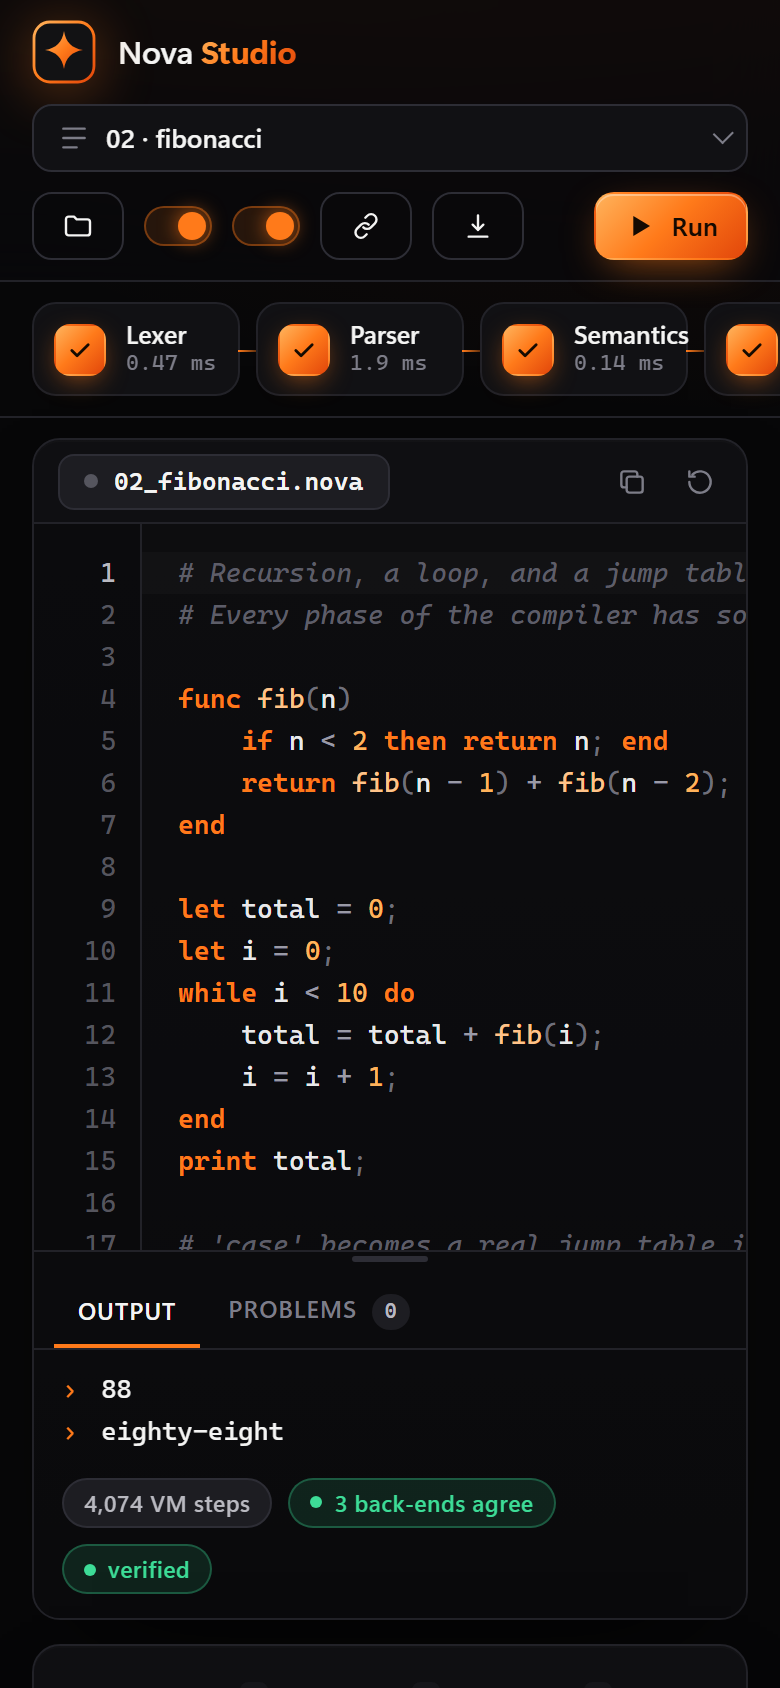
\includegraphics[width=0.44\columnwidth]{figures/mobile-overview.png}\label{fig:mobile-a}}
\hfil
\subfloat[VM stepper]{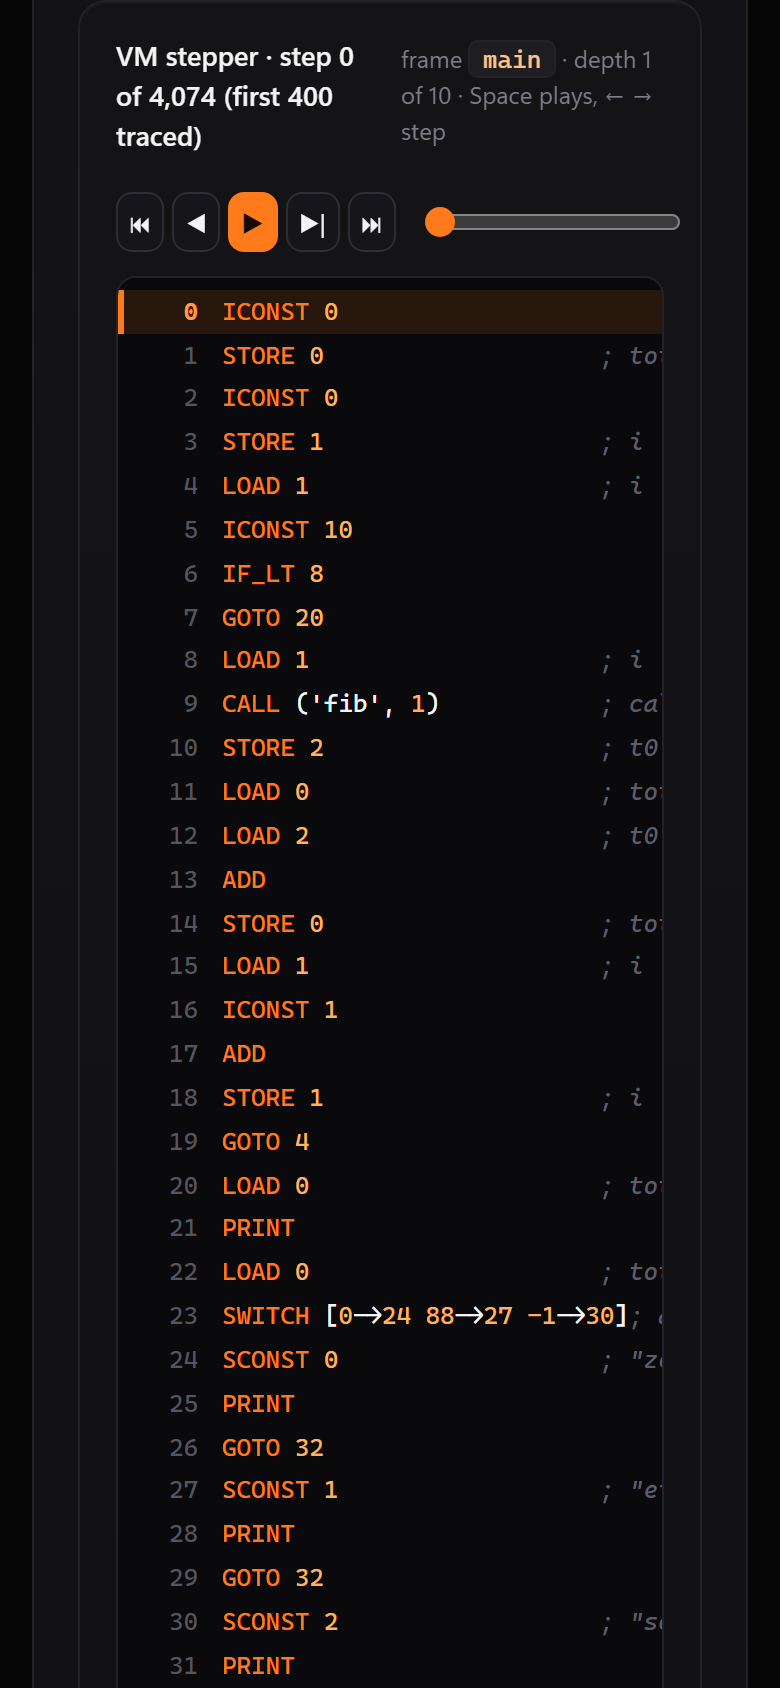
\includegraphics[width=0.44\columnwidth]{figures/mobile-stepper.png}\label{fig:mobile-b}}
\caption{The studio at a phone width of 390 pixels. The panes stack, the toolbar wraps, the pipeline rail scrolls sideways, and the instruments keep working.}
\label{fig:mobile}
\end{figure}

\begin{figure*}[!t]
\centering

\includegraphics[width=\textwidth]{figures/pipeline-rail.png}
\caption{The pipeline rail for the Fibonacci program: lexer, parser, semantic analysis, three-address code, optimiser, code generator, SSA, verifier and execution, each with its status and cost. Code generation and SSA run inside the same timed region as the optimiser and are reported as such.}
\label{fig:rail}
\end{figure*}

\begin{figure*}[!t]
\centering
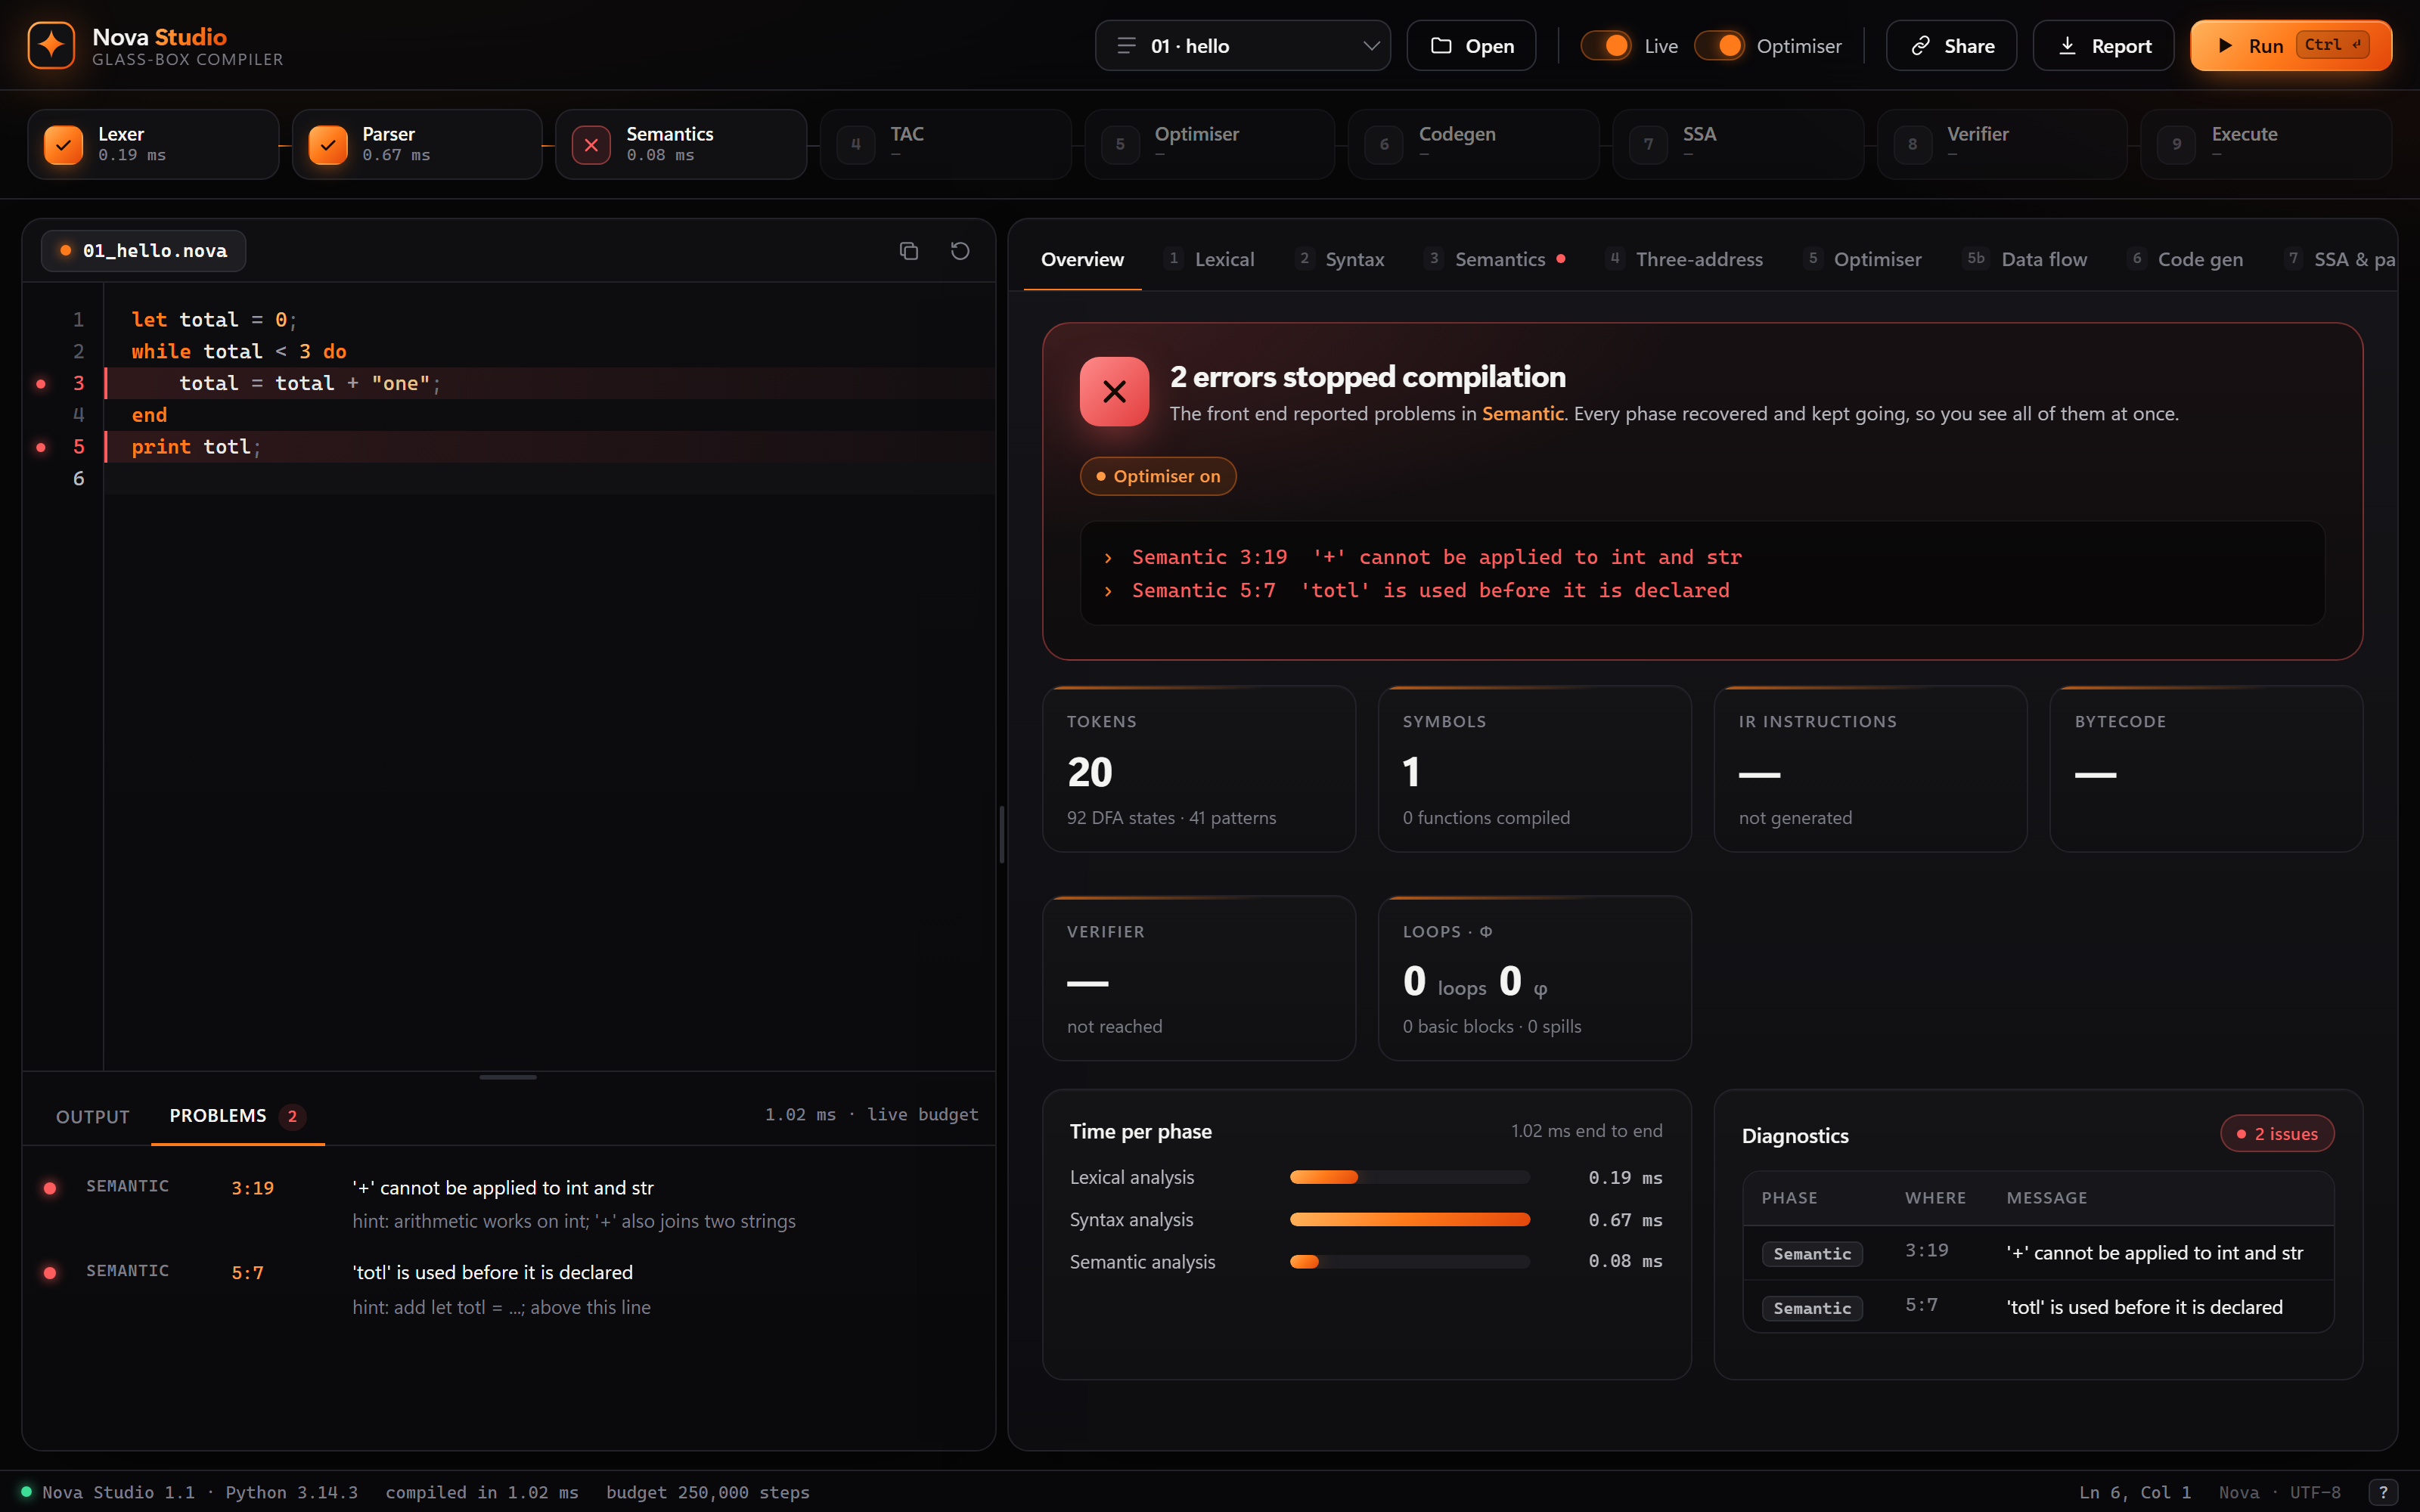
\includegraphics[width=\textwidth]{figures/live-error.png}
\caption{Live compilation catching two semantic errors as they are typed. Semantic analysis is marked failed and the later stages skipped; the summary, the gutter and the problems panel all point at line 3 (\code{'+' cannot be applied to int and str}) and line 5 (\code{'totl' is used before it is declared}), each with a hint. The status bar shows the live budget of 250,000 instructions.}
\label{fig:liveerror}
\end{figure*}

\begin{figure}[!t]
\centering
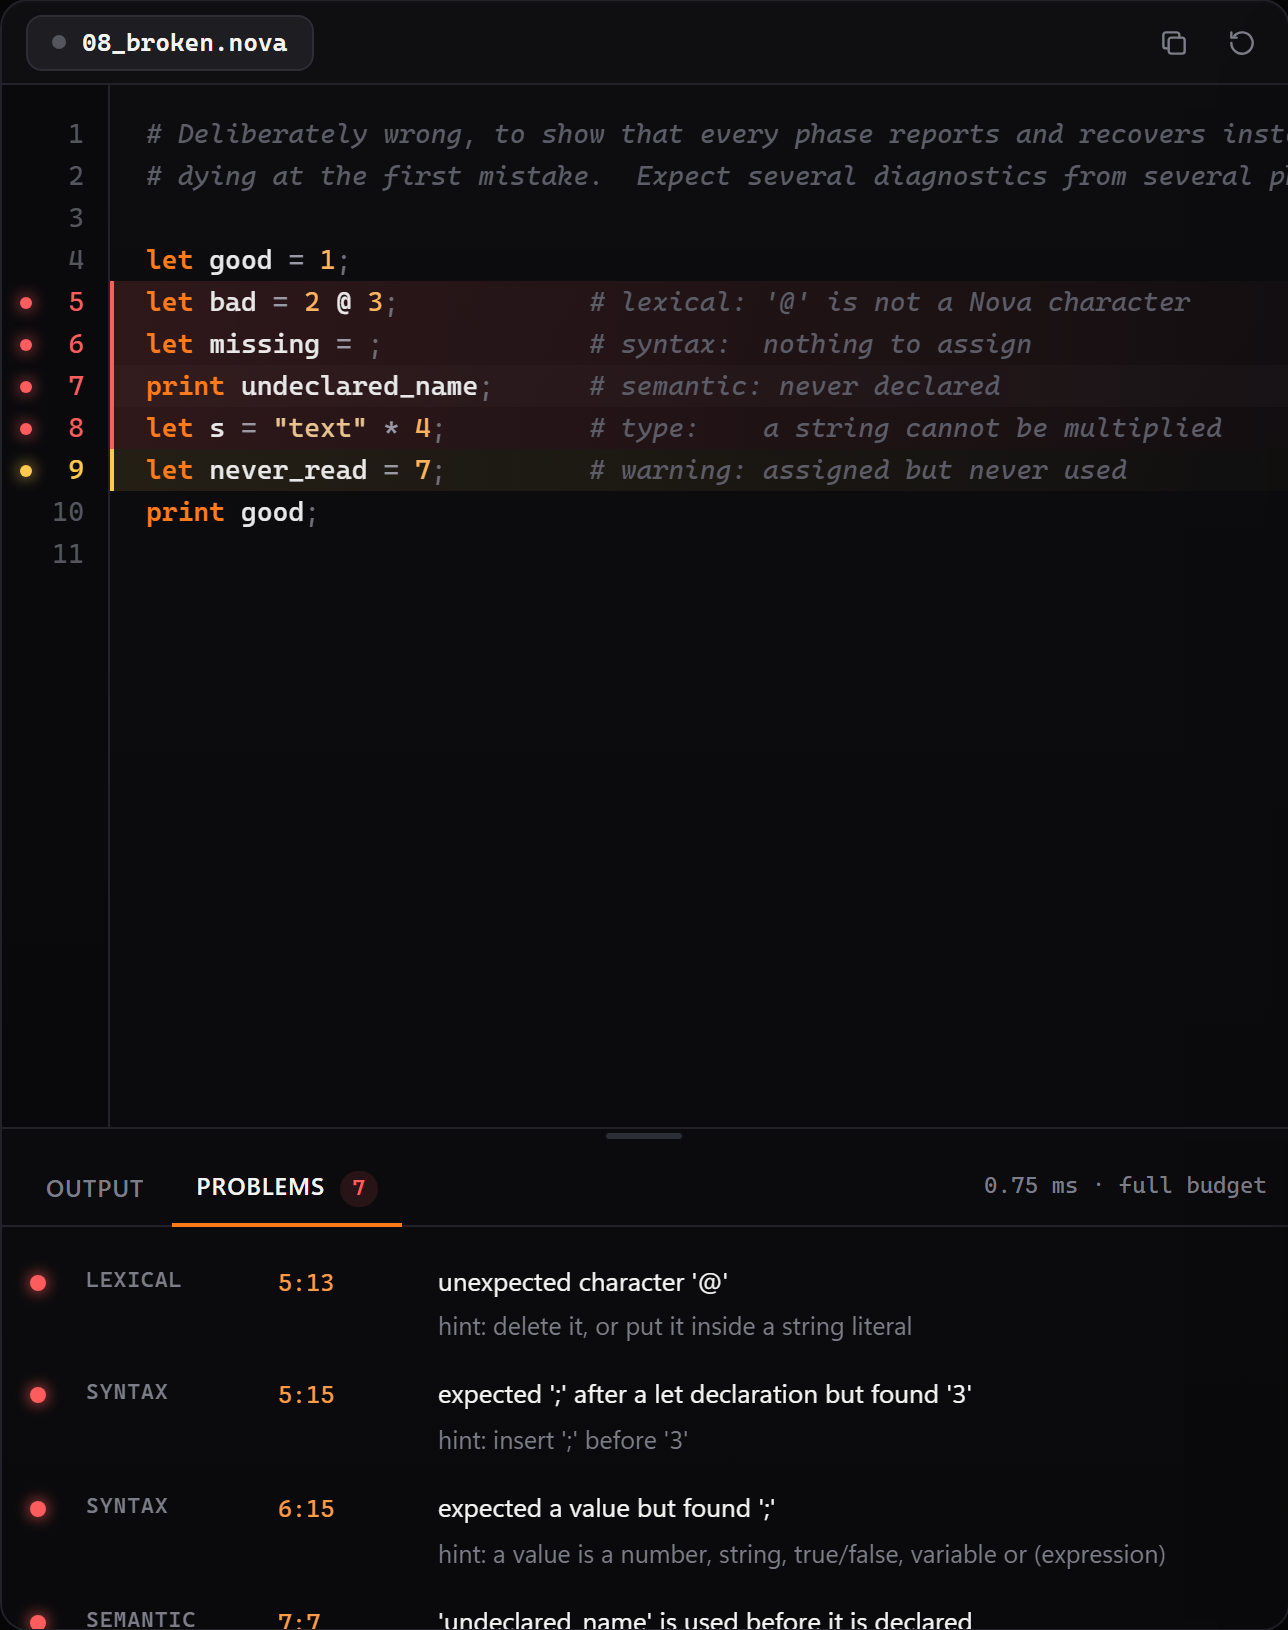
\includegraphics[width=0.88\columnwidth]{figures/editor-problems.png}
\caption{The editor and problems panel on \code{08\_broken.nova}. Error lines are marked red in the gutter and the warning line amber; each problem gives its phase, position, message and hint, and clicking one moves the caret to it.}
\label{fig:editorproblems}
\end{figure}

\begin{figure*}[!t]
\centering
\subfloat[Time per phase for the Fibonacci program, the bar lengths proportional to the cost of each phase]{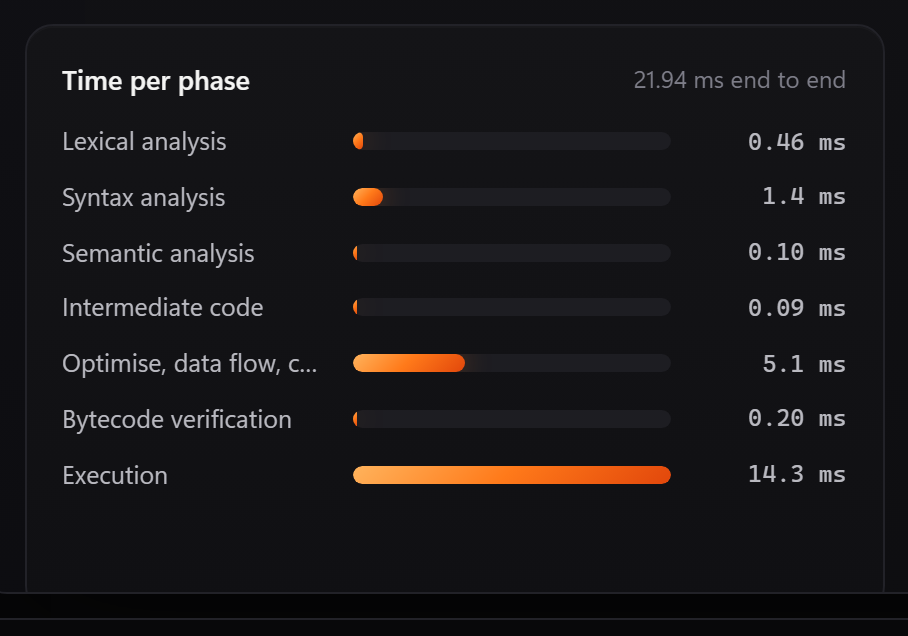
\includegraphics[width=0.41\textwidth]{figures/phase-times.png}\label{fig:panels-a}}
\hfil
\subfloat[The three back-ends on \code{03\_gcd.nova}: optimised and unoptimised stack bytecode (100 steps each) and the register machine (91 steps) all print \code{21 | 42}]{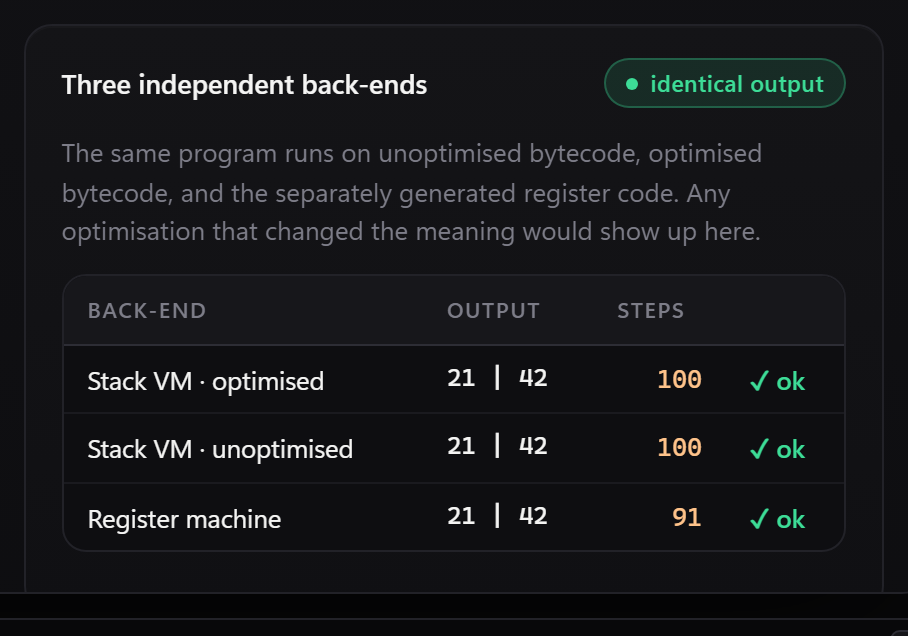
\includegraphics[width=0.41\textwidth]{figures/backends-gcd.png}\label{fig:panels-b}}
\caption{Two panels of the overview at full size.}
\label{fig:panels}
\end{figure*}

\begin{figure}[!t]
\centering
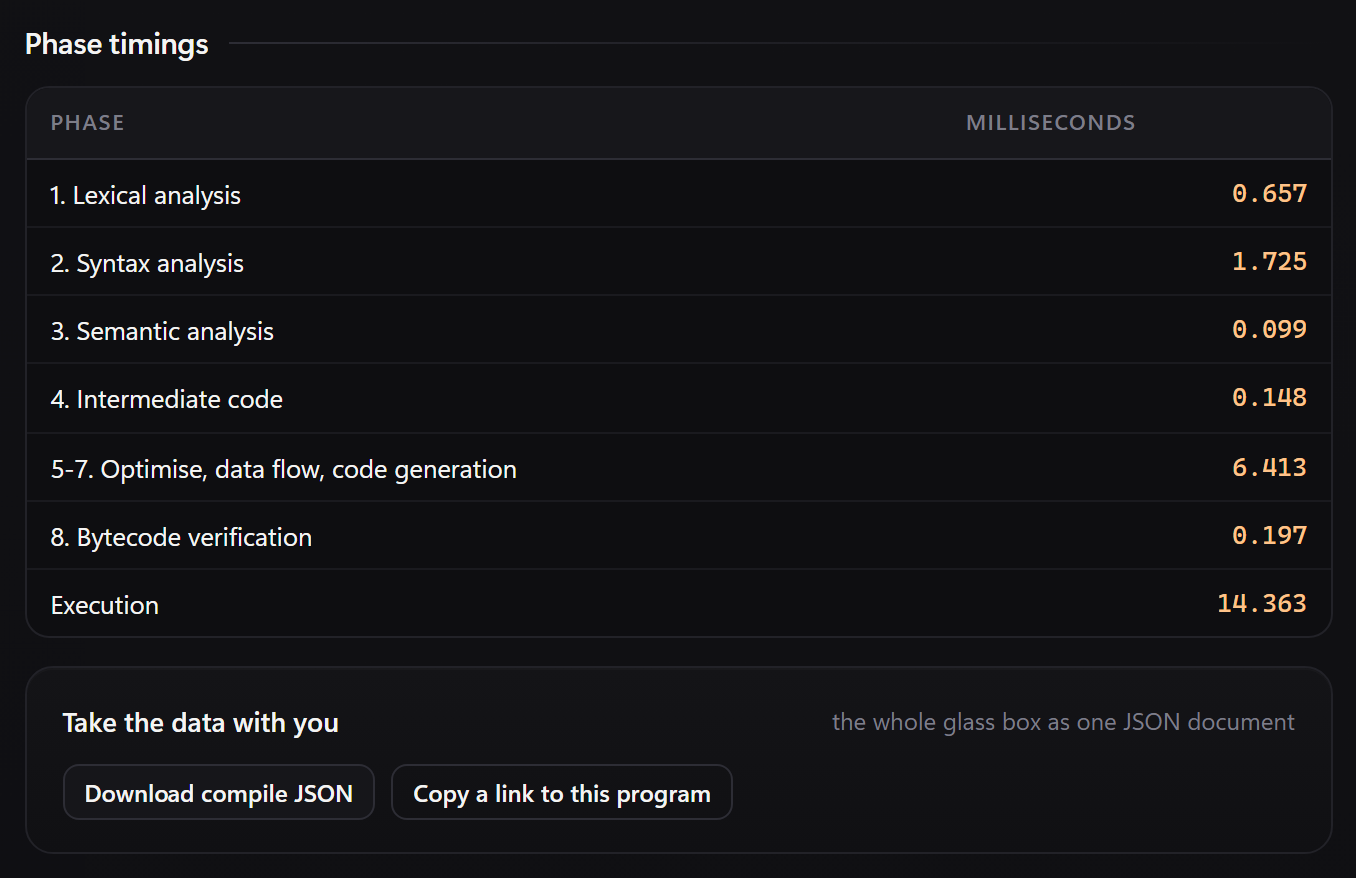
\includegraphics[width=0.8\columnwidth]{figures/metrics-timings.png}
\caption{The end of the metrics view: the time of every phase of the current compilation in milliseconds, and the buttons that download the complete compile JSON or copy a link that carries the whole program.}
\label{fig:metricstimings}
\end{figure}

\emph{Security model.} A development server on \code{localhost} can be reached by any web page that the user visits. Nova Studio therefore applies six controls:
\begin{itemize}
\item it binds to the loopback interface;
\item it accepts only \code{application/json} POST bodies, which forces a cross-origin preflight that the server never grants~\cite{fetchspec};
\item it rejects requests whose \code{Host} header does not name the loopback interface, which defeats DNS rebinding~\cite{jackson2007};
\item it caps request bodies at 512\,KB;
\item it sends a restrictive Content Security Policy~\cite{csp3} and \code{nosniff} headers;
\item it versions its assets by content hash, so browsers never execute stale code.
\end{itemize}

\subsection{Command-Line Interface and a Worked Example}
\label{sec:cli}
Every artefact is also available without a browser. The command-line interface (Table~\ref{tab:cli}) prints one phase, or all of them, for a source file; the self-test and the hostile-bytecode demonstration run from the same entry point. We follow \code{03\_gcd.nova} (Fig.~\ref{fig:gcdsrc}) through it. The program defines Euclid's algorithm and a least-common-multiple function that calls it, and prints $\gcd(1071, 462) = 21$ and $\mathrm{lcm}(21, 6) = 42$ (Fig.~\ref{fig:clirun}).

\begin{table}[!t]
\caption{Command-Line Interface (\code{python -m nova \ldots})}
\label{tab:cli}
\centering
\footnotesize
\setlength{\tabcolsep}{3.5pt}
\begin{tabular}{@{}l L{5.0cm}@{}}
\toprule
Command & Prints \\
\midrule
\code{run} \emph{file} & compile, verify and execute; the program's output \\
\code{phases} \emph{file} & every phase, in order \\
\code{tokens} \emph{file} & DFA statistics and the token stream \\
\code{ir} \emph{file} & TAC, the pass-by-pass optimisation and the flow graph \\
\code{asm} \emph{file} & activation records and register-machine code \\
\code{bytecode} \emph{file} & stack bytecode and the verifier's report \\
\code{llvm} \emph{file} & textual LLVM IR \\
\code{metrics} \emph{file} & the measurement table \\
\code{report} \emph{file} & writes the self-contained HTML report \\
\code{gui} [\emph{file}] & opens the desktop viewer \\
\code{serve} [\code{--port} $N$] & starts Nova Studio \\
\code{attack} & hostile bytecode against verifier and sandbox \\
\code{test} & the 34-test self-check \\
\bottomrule
\end{tabular}
\end{table}

\begin{figure}[!t]
\lstinputlisting[firstline=4]{data/cli/src-gcd.txt}
\caption{\code{03\_gcd.nova}: Euclid's algorithm with a loop at the very start of \code{gcd}, and \code{lcm} calling it, so that two activation records are live at once.}
\label{fig:gcdsrc}
\end{figure}

\begin{figure}[!t]
\lstinputlisting[style=term]{data/cli/run-gcd.txt}
\caption{\code{python -m nova run examples/03\_gcd.nova}: the program's output, produced by the verified optimised bytecode.}
\label{fig:clirun}
\end{figure}

\emph{Three-address code and optimisation.} \code{nova ir} prints the TAC of each function, the ten pass records and the optimised flow graph (Fig.~\ref{fig:cliir}). The loop of \code{gcd} is seven quadruples; it contains no redundancy, so every pass reports zero changes---the same result as Table~\ref{tab:onoff}---and the flow graph has four blocks, with \code{B0} both the entry and the loop header.

\emph{Register-machine code.} \code{nova asm} prints each function's activation record and the code produced by the next-use allocator (Fig.~\ref{fig:cliasm}). In \code{gcd}, \code{b} is loaded into \code{R0} once per iteration, the copy \code{t = b} becomes a register move, the remainder is computed in place in \code{R2}, and the two live values are stored back to the frame before the jump to the header, because every block is generated independently.

\emph{Bytecode and verification.} \code{nova bytecode} prints the stack code and then the verifier's report (Fig.~\ref{fig:clibc}): fifteen instructions for \code{gcd}, and six properties proved for each of its three functions, with a maximum stack depth of two everywhere.

\emph{Diagnostics.} On \code{08\_broken.nova} the same command prints all seven diagnostics with their phase, position and hint, and labels the two unused-variable reports as warnings rather than errors (Fig.~\ref{fig:clibroken}). The labelling was itself corrected during this work: the command line had printed every diagnostic as an error, while the studio and the HTML report distinguished warnings.

\emph{Attacks and self-test.} \code{nova attack} hands the eight hostile programs to the verifier and the VM and prints what stopped each (Fig.~\ref{fig:cliattack}); \code{nova test} runs the 34 self-tests, whose complete output is reproduced in Appendix~\ref{app:tests}.

\begin{figure}[!t]
\lstinputlisting[style=term, firstline=1, lastline=41]{data/cli/ir-gcd.txt}
\caption{\code{python -m nova ir} on \code{03\_gcd.nova}, the part for \code{gcd}: the three-address code, the ten pass records (none changes the code) and the optimised flow graph.}
\label{fig:cliir}
\end{figure}

\begin{figure}[!t]
\lstinputlisting[style=term, firstline=1, lastline=23]{data/cli/asm-gcd.txt}
\caption{\code{python -m nova asm} on \code{03\_gcd.nova}, the part for \code{gcd}: the activation record (return address, control link, two parameters and a local) and thirteen register-machine instructions with the allocator's comments.}
\label{fig:cliasm}
\end{figure}

\begin{figure}[!t]
\lstinputlisting[style=term, firstline=1, lastline=20]{data/cli/bytecode-gcd.txt}
\vspace{2pt}
\lstinputlisting[style=term, firstline=54, lastline=62]{data/cli/bytecode-gcd.txt}
\caption{\code{python -m nova bytecode} on \code{03\_gcd.nova}: the stack bytecode of \code{gcd} (top) and the verifier's report for it (bottom). The full output continues with \code{lcm} and \code{main}, which are also verified.}
\label{fig:clibc}
\end{figure}

\begin{figure}[!t]
\lstinputlisting[style=term]{data/cli/run-broken.txt}
\caption{\code{python -m nova run} on \code{08\_broken.nova}: five errors and two warnings from three phases in one run, each with a hint.}
\label{fig:clibroken}
\end{figure}

\begin{figure}[!t]
\lstinputlisting[style=term, firstline=30, lastline=45]{data/cli/attack.txt}
\caption{The end of \code{python -m nova attack}: attacks 6--8 and the summary. The frame escape is rejected statically; the two denials of service pass verification and are stopped by the sandbox.}
\label{fig:cliattack}
\end{figure}

\subsection{Evaluation Methodology}
\label{sec:evalmethod}
\emph{Benchmarks.} The suite in Table~\ref{tab:bench} contains eleven programs, each chosen to exercise particular phases; \code{08\_broken.nova} contains one deliberate mistake per front-end phase, and \code{11\_deep\_recursion.nova} recurses 200 deep, inside the sandbox's limit of 256 frames. A synthetic series of programs made of 1 to 64 copies of a seven-line loop measures how compile time scales with program size.

\begin{table}[!t]
\caption{Benchmark Programs}
\label{tab:bench}
\centering
\footnotesize
\setlength{\tabcolsep}{3.5pt}
\begin{tabular*}{\columnwidth}{@{\extracolsep{\fill}}l r r r L{3.65cm}@{}}
\toprule
Program & LOC$^{a}$ & Tokens & Fn. & Exercises \\
\midrule
\code{hello} & 4 & 18 & 1 & smallest complete program \\
\code{fibonacci} & 16 & 84 & 2 & recursion, loop, jump table \\
\code{gcd} & 13 & 68 & 3 & nested calls; loop at function entry \\
\code{primes} & 20 & 103 & 2 & nested loops, short-circuit \code{and} \\
\code{optimiser} & 18 & 97 & 2 & CSE, LICM, strength reduction, DCE \\
\code{parallel} & 23 & 102 & 1 & three loops with different dependences \\
\code{types} & 22 & 104 & 2 & shadowing, scopes, booleans \\
\code{broken} & 7 & 33 & 0 & one error per front-end phase \\
\code{nested} & 13 & 60 & 1 & a nested loop pair; locality advice \\
\code{strings} & 19 & 88 & 2 & strings, booleans, \code{if}/\code{else} in a function, \code{otherwise} \\
\code{recursion} & 10 & 62 & 3 & 200 nested activation records \\
\bottomrule
\end{tabular*}
\par\vspace{0pt}
\parbox{\columnwidth}{\scriptsize $^{a}$Non-blank, non-comment lines; ``Fn.'' counts compiled functions including \code{main}. Program \code{x} is the file \code{examples/NN\_x.nova}; \code{types} is \code{07\_types\_and\_scopes.nova}, \code{nested} is \code{09\_nested\_loops.nova} and \code{recursion} is \code{11\_deep\_recursion.nova}.}
\end{table}

\emph{Metrics and measurement protocol.} Structural metrics are read from the \code{CompileResult}. Compile times are medians of 60 warm runs measured with a high-resolution wall clock and cross-checked against process CPU time; LR table construction times are medians of three runs with a fresh builder; scaling times are medians of 25 runs (12 for the two largest programs); HTTP round trips are medians of 30 requests over one keep-alive connection to a separate server process, which is how a browser uses the studio. The measurement script records the machine's power state, because a laptop on battery runs its processor more slowly. The script \code{report/tools/measure.py} produces every number in Section~\ref{sec:results}; \code{report/tools/capture.mjs} produces every studio screenshot by driving Nova Studio through the Chrome DevTools protocol at twice the display density, and \code{report/tools/desktop\_capture.ps1} photographs the desktop viewer's own window.

\emph{Correctness.} A self-test suite of 34 tests (Table~\ref{tab:tests}) combines four kinds of evidence:
\begin{itemize}
\item textbook checks, for example that the DFA for $(a|b)^{*}abb$ has four states;
\item differential tests across the three back-ends and with the optimiser on and off, for all ten valid programs;
\item the hostile-bytecode suite;
\item HTTP API tests and regression tests for every defect reported in Section~\ref{sec:res-defects}.
\end{itemize}
Every view of the studio is also exercised for every example program by a headless browser that records any page error; the capture of the figures in this report doubled as that test, and no error was recorded.

\begin{table}[!t]
\caption{Self-Test Suite (34 Tests)}
\label{tab:tests}
\centering
\footnotesize
\setlength{\tabcolsep}{3.5pt}
\begin{tabular}{@{}l r L{5.75cm}@{}}
\toprule
Group & $n$ & What is checked \\
\midrule
M1 & 3 & direct-method DFA; minimisation; maximal munch and keyword priority \\
M2 & 6 & FIRST/FOLLOW; left recursion; ambiguity conflicts; SLR/CLR/LALR accept Nova; LALR agrees with recursive descent; table-cache regression \\
M3 & 3 & type errors; shadowing; function-use flags (regression) \\
M4 & 2 & short-circuit jumping code; jump tables and backpatching \\
M5 & 3 & killed copies are not propagated; optimiser removes code; data-flow fixed points \\
M6 & 3 & register and stack machines agree; optimised and unoptimised code agree; activation records \\
M7 & 3 & $\phi$ placement; $\phi$ at an entry loop header (regression); dependence verdicts \\
M8 & 3 & honest bytecode passes; every hostile program is stopped; no false rejection \\
E2E & 6 & expected outputs of ten programs; multi-phase diagnostics; HTML report; optimiser switch; deep nesting; budgets \\
WEB & 2 & JSON for every example; HTTP API with its 400/403/404/415 guards \\
\bottomrule
\end{tabular}
\end{table}

% =============================================================================
\section{Results and Discussion}
\label{sec:results}

\subsection{Experimental Setup}
All measurements were taken on a laptop with a 13th-generation Intel Core i5-13500HX processor (14 cores, 20 threads), 15.7\,GB of memory and Windows~11 (build 26200), using CPython 3.14.3. The laptop was running on \emph{battery} under its vendor power plan, which throttles the processor; an earlier session on mains power ran the same compilations roughly $3.5\times$ faster. All timings in this section are therefore conservative, and the ratios between them, not the absolute values, are the durable findings. Screenshots were rendered by Chrome 155 driven from Node.js 24. All 34 self-tests pass.

\subsection{Lexical and Syntactic Analysis}
\label{sec:res-front}
Table~\ref{tab:front} summarises the front end. The direct method produces a 92-state DFA that Moore's refinement cannot reduce further: building the automaton from position sets yields no equivalent states for this specification. The scanner trace confirms the intended priority rule on real tokens: in Fig.~\ref{fig:scanner-func} the path of \code{func} passes through three states that accept \code{IDENT} before ending in state 74, which accepts both \code{IDENT} and \code{FUNC} and reports \code{FUNC} because the keyword pattern has the lower index, whereas \code{total} (Fig.~\ref{fig:scanner-ident}) enters the generic identifier state 19 after its first character and stays there.

The Nova grammar has 77 multiply defined LL(1) entries, most of which come from left recursion. After left-recursion elimination the grammar grows to 69 productions over 31 non-terminals, and four conflicts remain. All four are common-prefix conflicts (\code{IDENT} followed by an assignment or a call, \code{if} with or without \code{else}, \code{case} with or without \code{otherwise}, and a variable or a call in an expression) that left factoring removes---the same situations in which the hand-written parser looks one token further.

\begin{table}[!t]
\caption{Front-End Statistics}
\label{tab:front}
\centering
\footnotesize
\setlength{\tabcolsep}{4pt}
\begin{tabular*}{\columnwidth}{@{\extracolsep{\fill}}l r@{}}
\toprule
\multicolumn{2}{@{}l}{\emph{Scanner}} \\
Token patterns / keywords & 41 / 19 \\
Positions in the combined syntax tree & 147 \\
DFA states before / after minimisation & 92 / 92 \\
Symbol equivalence classes & 37 \\
\midrule
\multicolumn{2}{@{}l}{\emph{Grammar}} \\
Productions / terminals / non-terminals & 58 / 39 / 20 \\
LL(1) conflicts, as written & 77 \\
LL(1) conflicts after left-recursion elimination & 4 \\
Ambiguous expression grammar: shift/reduce conflicts & 4 \\
\bottomrule
\end{tabular*}

\vspace{6pt}
\begin{tabular*}{\columnwidth}{@{\extracolsep{\fill}}l r r r r@{}}
\toprule
LR table & States & Entries & Conflicts & Build (ms) \\
\midrule
SLR(1) & 116 & 1,229 & 0 & 38.1 \\
CLR(1) & 478 & 4,790 & 0 & 1,771.6 \\
LALR(1) & 116 & 1,214 & 0 & 1,798.7 \\
\bottomrule
\end{tabular*}
\end{table}

The LR results reproduce the classical trade-off with real numbers. On this grammar, SLR(1), CLR(1) and LALR(1) all produce conflict-free tables, so the extra power of LR(1) look-aheads is not needed. CLR(1), however, splits the automaton into 478 states with 4,790 entries, whereas LALR(1) keeps SLR(1)'s 116 states and has 1,214 entries---75\% fewer than CLR(1), and even 15 fewer than SLR(1), because merged LR(1) look-aheads are more precise than FOLLOW sets. This is the argument for LALR(1) in Yacc and Bison~\cite{johnson1975,bison}, now measured rather than quoted. The automaton browser makes the merged look-aheads concrete: state 2 in Fig.~\ref{fig:automaton} carries the look-ahead set $\{\$, \code{CASE}, \code{FUNC}, \ldots\}$ on every statement item, the union of the look-aheads of the LR(1) states that were merged into it.

Construction cost tells a second story. Because Nova obtains LALR(1) by merging CLR(1) states~\eqref{eq:lalr}, it pays the full price of the canonical collection (1,798.7\,ms against 38.1\,ms for SLR(1), a factor of 47), which is exactly why production generators compute LALR look-aheads directly from the LR(0) automaton~\cite{deremer1982}. The cost is incurred once, when the server starts (3.8\,s for all three tables on this machine), and is then cached.

The LALR(1) driver accepted every valid benchmark and rejected \code{broken}, in agreement with the recursive-descent parser; the bottom-up parses take 68--383 steps (Table~\ref{tab:programs}). On the ambiguous expression grammar, SLR(1) construction reports four shift/reduce conflicts, two in each of states 8 and 9 on \code{+} and \code{*} (Fig.~\ref{fig:ambiguous}), which is the expected signature of missing precedence and associativity. The parse player (Fig.~\ref{fig:player}) shows the same machinery from the driver's side: at step 32 the reduction \code{unary $\to$ factor} is dictated by the single kernel item of state 25, whose look-ahead set contains the look-ahead \code{;}.

\subsection{End-to-End Compilation}
Table~\ref{tab:programs} reports every phase for every benchmark. All ten valid programs compile, pass verification and run, and every property check succeeds (114 of 114). The intermediate code ranges from 6 to 38 quadruples per program (243 in total) with 58 backpatch operations, and SSA construction places 39 $\phi$-functions across the suite. The front end recovers from errors in \code{broken} and stops before code generation, as designed. Compile times are 1.97--36.3\,ms for nine of the ten valid programs; the tenth, \code{recursion}, takes 194.8\,ms, of which 181.5\,ms is execution---the program runs three times, and the VM re-renders the whole activation-record stack every time a new maximum depth is reached, which for a recursion 200 deep is 20,100 frame renderings. That cost is the price of the deepest-stack snapshot of Fig.~\ref{fig:deeprec}, and it is discussed as a limitation in Section~\ref{sec:res-perf}.

\begin{table*}[!t]
\caption{Compilation Results per Benchmark (Median Compile Time over 60 Runs, Battery Power)}
\label{tab:programs}
\centering
\scriptsize
\setlength{\tabcolsep}{4.6pt}
\begin{tabular*}{\textwidth}{@{\extracolsep{\fill}}l r r r r r r r r r r r r r r@{}}
\toprule
Program & Tokens & LR steps & Symbols & TAC & Backp. & Blocks & IR & Loops & $\phi$ & Target & Spills & Bytecode & Checks & ms \\
\midrule
\code{hello} & 18 & 68 & 2 & 6 & 0 & 1 & 6$\to$3 & 0 & 0 & 5 & 0 & 14$\to$6 & 6/6 & 1.97 \\
\code{fibonacci} & 84 & 297 & 4 & 28 & 6 & 13 & 28$\to$28 & 1 & 3 & 61 & 0 & 60$\to$60 & 12/12 & 36.27 \\
\code{gcd} & 68 & 239 & 7 & 22 & 2 & 6 & 22$\to$22 & 1 & 3 & 42 & 0 & 43$\to$43 & 18/18 & 10.55 \\
\code{primes} & 103 & 363 & 6 & 31 & 11 & 21 & 31$\to$31 & 2 & 9 & 68 & 0 & 71$\to$71 & 12/12 & 28.57 \\
\code{optimiser} & 97 & 318 & 11 & 21 & 2 & 6 & 21$\to$19 & 1 & 4 & 42 & 1 & 55$\to$47 & 12/12 & 15.37 \\
\code{parallel} & 102 & 363 & 5 & 28 & 6 & 13 & 28$\to$26 & 3 & 7 & 56 & 0 & 67$\to$63 & 6/6 & 18.36 \\
\code{types} & 104 & 383 & 6 & 38 & 12 & 22 & 38$\to$31 & 1 & 5 & 62 & 0 & 78$\to$60 & 12/12 & 19.72 \\
\code{broken} & 33 & 22 & 3 & \multicolumn{10}{c}{\textit{stopped after semantic analysis: 5 errors, 2 warnings}} & 0.90 \\
\code{nested} & 60 & 206 & 5 & 17 & 4 & 9 & 17$\to$15 & 2 & 7 & 32 & 0 & 40$\to$36 & 6/6 & 13.32 \\
\code{strings} & 88 & 314 & 6 & 29 & 11 & 19 & 29$\to$25 & 0 & 1 & 50 & 0 & 57$\to$46 & 12/12 & 12.04 \\
\code{recursion} & 62 & 227 & 4 & 23 & 4 & 9 & 23$\to$23 & 0 & 0 & 47 & 0 & 50$\to$50 & 18/18 & 194.81 \\
\bottomrule
\end{tabular*}
\par\vspace{0pt}
\parbox{\textwidth}{\scriptsize TAC: three-address instructions; Backp.: backpatch operations; IR: instructions before$\to$after optimisation; Target: register-machine instructions; Bytecode: unoptimised$\to$optimised instructions; Checks: verifier properties proved; ms: median compile time including three executions and LLVM emission.}
\end{table*}

\subsection{Optimisation Effectiveness}
Table~\ref{tab:passes} traces \code{main} of the \code{optimiser} benchmark pass by pass, and Fig.~\ref{fig:cfg} shows its flow graph before and after. The first three passes change the code without changing its size: value numbering reuses one common subexpression (the shared node \code{n2} of Fig.~\ref{fig:dag}) and folds one constant, and constant propagation substitutes one operand. LICM hoists the invariant product \code{width*height} into a preheader. Strength reduction then \emph{adds} an instruction, introducing an incrementally updated induction variable in place of \code{i*8}, and dead-code elimination removes three instructions that had become dead, among them the definition of \code{n} after constant propagation and the never-read \code{unused}. The net effect is 20$\to$18 instructions in \code{main}. The waterfall in Fig.~\ref{fig:optimiser} makes this non-monotone behaviour visible, where a single before-and-after count would hide it.

\begin{table}[!t]
\caption{Pass-by-Pass Optimisation of \code{main} in \code{optimiser}}
\label{tab:passes}
\centering
\scriptsize
\setlength{\tabcolsep}{3pt}
\begin{tabular}{@{}l r r r L{2.75cm}@{}}
\toprule
Pass & Before & After & $\Delta$ & Effect \\
\midrule
Local value numbering & 20 & 20 & 0 & 1 CSE reused, 1 constant folded \\
Constant propagation & 20 & 20 & 0 & 1 operand replaced \\
Copy propagation & 20 & 20 & 0 & no copy replaced \\
Loop-invariant motion & 20 & 20 & 0 & 1 instruction hoisted \\
Strength reduction & 20 & 21 & $+1$ & 1 induction variable reduced \\
Dead-code elimination & 21 & 18 & $-3$ & 3 dead instructions removed \\
Unreachable code & 18 & 18 & 0 & every block reachable \\
Jump optimisation & 18 & 18 & 0 & no jump changed \\
Value numbering (2nd) & 18 & 18 & 0 & 1 constant folded \\
Dead code (2nd) & 18 & 18 & 0 & nothing left to remove \\
\bottomrule
\end{tabular}
\end{table}

Table~\ref{tab:onoff} compares each program compiled with the optimiser switched off and on. The optimiser shrinks the intermediate code by up to 50\%, the bytecode by up to 57\% and the number of executed VM instructions by up to 57\%. The largest reductions come from the smallest program, whose constant expressions fold away entirely; the largest on substantial programs are 23\% (bytecode) and 25\% (executed instructions) for \code{types}, and 19\% and 25\% for \code{strings}, where the \code{if}/\code{else} inside \code{greet} and the boolean expression leave dead temporaries and copies for the passes to remove. Four programs---\code{fibonacci}, \code{gcd}, \code{primes} and \code{recursion}---are unchanged: written idiomatically, they contain no redundancy for the classical machine-independent passes to remove, which is itself a useful lesson that optimisers mostly repair inefficient code. The \code{nested} benchmark shows the other extreme of the relation between static and dynamic savings: 10\% fewer bytecode instructions but only 2\% fewer executed, because the instructions removed lie outside the inner loop. Most importantly, every program prints exactly the same output with the optimiser on and off (Fig.~\ref{fig:switch}).

\begin{table}[!t]
\caption{Effect of the Optimiser (Off $\to$ On)}
\label{tab:onoff}
\centering
\footnotesize
\setlength{\tabcolsep}{2.6pt}
\begin{tabular}{@{}l r r r r r r r r r@{}}
\toprule
& \multicolumn{3}{c}{IR instructions} & \multicolumn{3}{c}{Bytecode} & \multicolumn{3}{c}{VM steps} \\
\cmidrule(lr){2-4}\cmidrule(lr){5-7}\cmidrule(l){8-10}
Program & off & on & \% & off & on & \% & off & on & \% \\
\midrule
\code{hello} & 6 & 3 & 50 & 14 & 6 & 57 & 14 & 6 & 57 \\
\code{fibonacci} & 28 & 28 & 0 & 60 & 60 & 0 & 4,074 & 4,074 & 0 \\
\code{gcd} & 22 & 22 & 0 & 43 & 43 & 0 & 100 & 100 & 0 \\
\code{primes} & 31 & 31 & 0 & 71 & 71 & 0 & 1,610 & 1,610 & 0 \\
\code{optimiser} & 21 & 19 & 10 & 55 & 47 & 15 & 188 & 148 & 21 \\
\code{parallel} & 28 & 26 & 7 & 67 & 63 & 6 & 340 & 336 & 1 \\
\code{types} & 38 & 31 & 18 & 78 & 60 & 23 & 114 & 85 & 25 \\
\code{nested} & 17 & 15 & 12 & 40 & 36 & 10 & 264 & 260 & 2 \\
\code{strings} & 29 & 25 & 14 & 57 & 46 & 19 & 44 & 33 & 25 \\
\code{recursion} & 23 & 23 & 0 & 50 & 50 & 0 & 3,609 & 3,609 & 0 \\
\bottomrule
\end{tabular}
\end{table}

\begin{figure*}[!t]
\centering
\subfloat[\code{10\_strings.nova}: string concatenation, a boolean, an \code{if}/\code{else} inside a function and a \code{case} with \code{otherwise}, all verified and agreed by the three back-ends.]{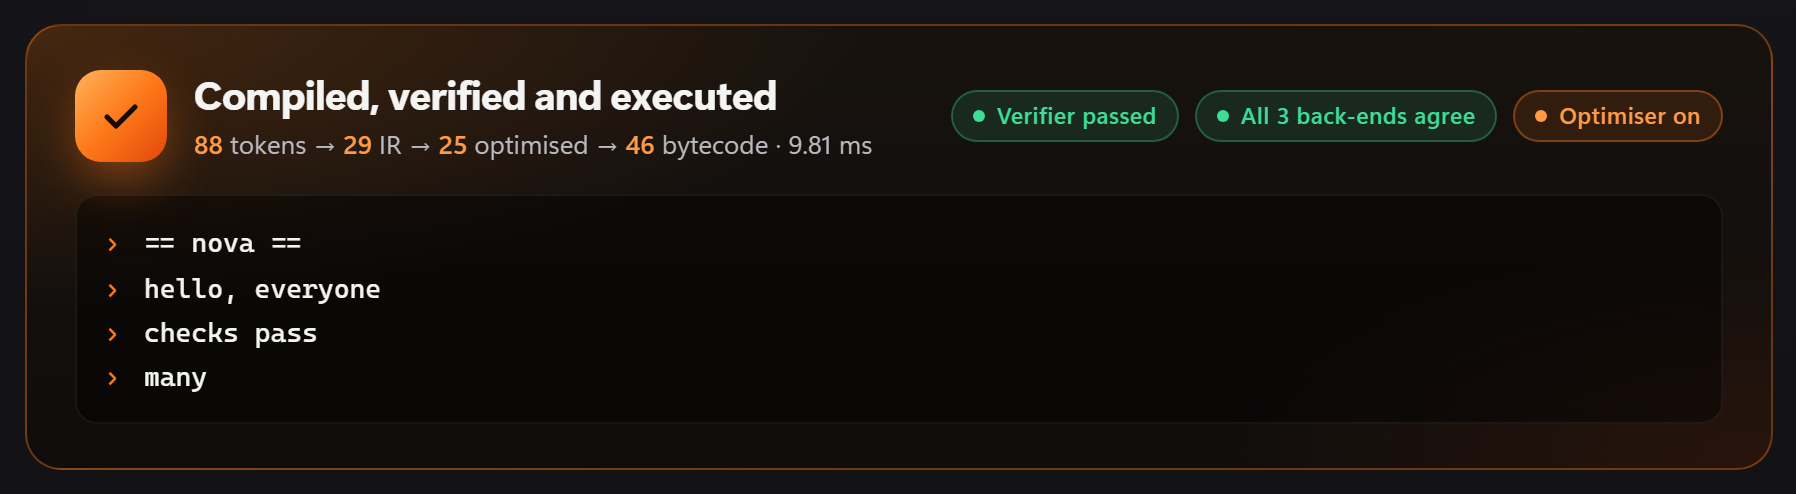
\includegraphics[width=0.49\textwidth]{figures/overview-strings.png}\label{fig:switch-a}}
\hfil
\subfloat[\code{05\_optimiser.nova} with the optimiser switched off: 21 IR and 55 bytecode instructions instead of 19 and 47, the same output \code{320}, and the switch's state shown in the summary.]{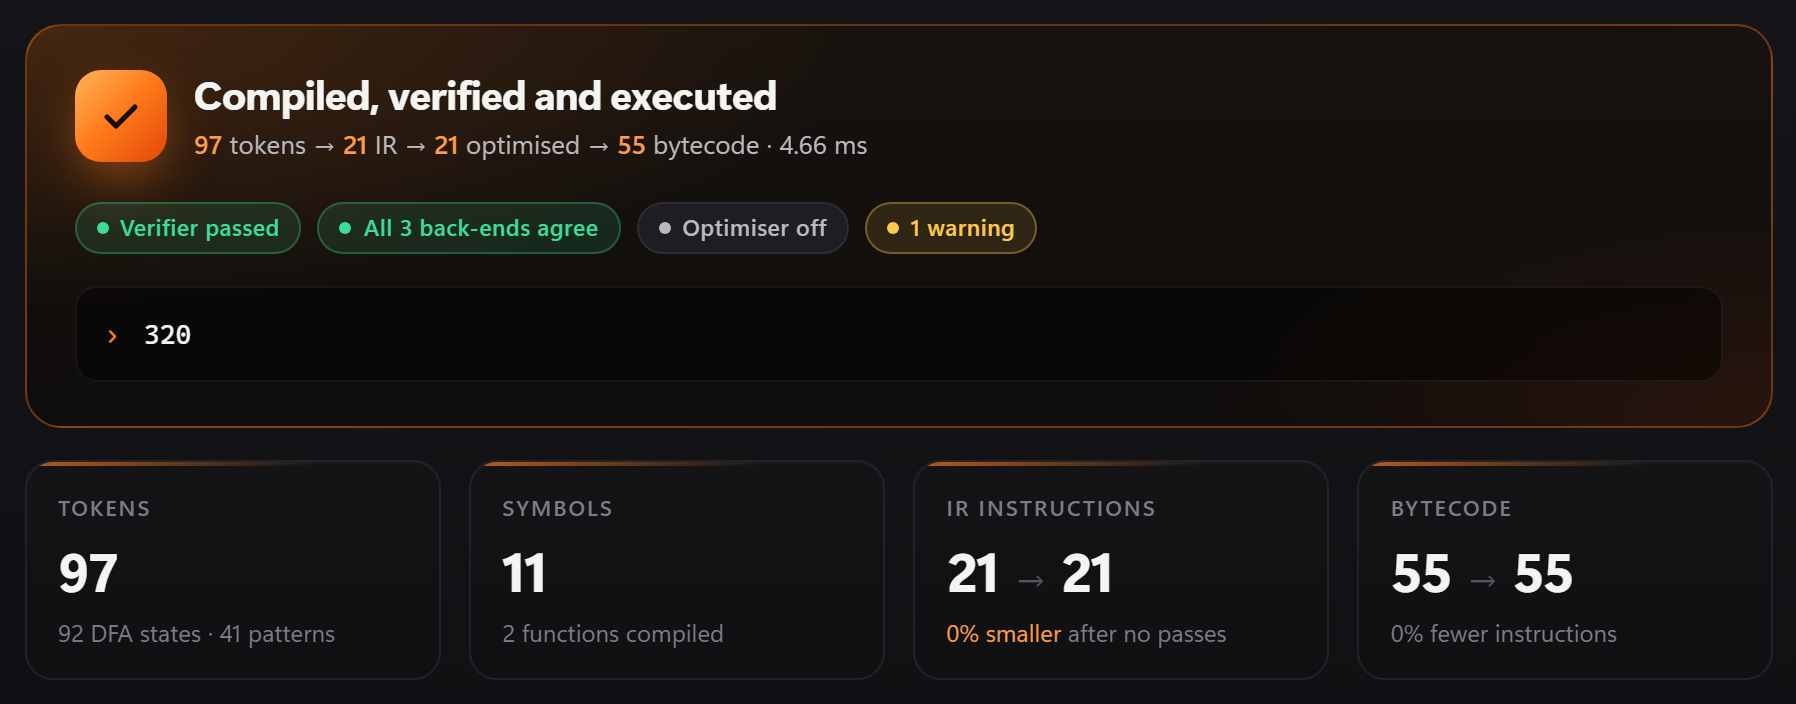
\includegraphics[width=0.49\textwidth]{figures/overview-optimiser-off.png}\label{fig:switch-b}}
\caption{Two overview summaries. The optimiser switch recompiles the program through the unoptimised path so that its effect, and the invariance of the output, can be seen directly.}
\label{fig:switch}
\end{figure*}

\subsection{Data-Flow Convergence}
Table~\ref{tab:rounds} lists the number of round-robin passes that each analysis needs, counting the final pass that confirms the fixed point. No analysis needs more than four passes on any function, and the only function that needs four is \code{main} of \code{nested}, whose two nested loops give its flow graph a loop-connectedness of $d=2$. This agrees with the bound of Kam and Ullman~\cite{kam1976}, under which rapid frameworks converge within $d+2$ passes of a depth-first ordering: every other benchmark has $d \le 1$ and converges within three. The visible convergence in Fig.~\ref{fig:dataflow}, and the facts on the graph in Fig.~\ref{fig:dfoverlay}, turn this theorem into something a student can watch.

\begin{table}[!t]
\caption{Passes to the Fixed Point per Function (Including the Confirming Pass)}
\label{tab:rounds}
\centering
\footnotesize
\setlength{\tabcolsep}{4pt}
\begin{tabular*}{\columnwidth}{@{\extracolsep{\fill}}l c c c c@{}}
\toprule
Program / function & RD & LV & AE & VB \\
\midrule
\code{hello}/\code{main} & 1 & 1 & 1 & 2 \\
\code{fibonacci}/\code{fib} & 2 & 2 & 2 & 2 \\
\code{fibonacci}/\code{main} & 2 & 3 & 2 & 1 \\
\code{gcd}/\code{gcd} & 2 & 3 & 2 & 1 \\
\code{gcd}/\code{lcm} & 2 & 2 & 1 & 2 \\
\code{gcd}/\code{main} & 1 & 1 & 1 & 1 \\
\code{primes}/\code{isprime} & 3 & 3 & 2 & 3 \\
\code{primes}/\code{main} & 3 & 3 & 2 & 1 \\
\code{optimiser}/\code{measure} & 2 & 2 & 1 & 1 \\
\code{optimiser}/\code{main} & 2 & 3 & 2 & 2 \\
\code{parallel}/\code{main} & 2 & 3 & 2 & 1 \\
\code{types}/\code{classify} & 2 & 2 & 1 & 1 \\
\code{types}/\code{main} & 2 & 3 & 2 & 2 \\
\code{nested}/\code{main} & 3 & 4 & 2 & 1 \\
\code{strings}/\code{greet} & 2 & 2 & 1 & 1 \\
\code{strings}/\code{main} & 2 & 2 & 2 & 2 \\
\code{recursion}/\code{depth} & 2 & 2 & 2 & 2 \\
\code{recursion}/\code{fact} & 2 & 2 & 2 & 2 \\
\code{recursion}/\code{main} & 1 & 1 & 1 & 1 \\
\bottomrule
\end{tabular*}
\par\vspace{0pt}
\parbox{\columnwidth}{\scriptsize RD: reaching definitions; LV: live variables; AE: available expressions; VB: very busy expressions.}
\end{table}

\subsection{Code Generation and Back-End Agreement}
\label{sec:res-backends}
Table~\ref{tab:backends} reports the three executions of each program. On every benchmark the unoptimised stack VM, the optimised stack VM and the register machine print identical output, which is the differential check of correctness~\cite{mckeeman1998}. Fig.~\ref{fig:gcdoverview} shows the check as the studio presents it for \code{gcd}: the summary records that the verifier passed and that all three back-ends agree, and Fig.~\ref{fig:panels-b} lists the three executions side by side. A single spill occurs in the whole suite (in \code{optimiser}), so four registers suffice for these programs; the timeline of Fig.~\ref{fig:timeline} shows why, since at most four values are live at once and constants occupy a register for a single instruction. The register machine executes 6--25\% fewer instructions than the optimised stack VM on nine of the ten programs, because it keeps values in registers instead of pushing and popping them. The exception is \code{types} (87 against 85 instructions), where the code generator stores live values back at block boundaries and the stack code needs no such stores. The recursive \code{fibonacci} reaches a depth of ten activation records, which Fig.~\ref{fig:execution} shows frame by frame, and \code{recursion} reaches 202 (Fig.~\ref{fig:deeprec}).

\begin{table}[!t]
\caption{Execution on the Three Back-Ends}
\label{tab:backends}
\centering
\footnotesize
\setlength{\tabcolsep}{3.4pt}
\begin{tabular}{@{}l r r r r r c@{}}
\toprule
& \multicolumn{2}{c}{Stack VM steps} & Register & Max & Max & \\
\cmidrule(lr){2-3}
Program & unopt. & opt. & steps & frames & stack & Agree \\
\midrule
\code{hello} & 14 & 6 & 5 & 1 & 1 & \cmark \\
\code{fibonacci} & 4,074 & 4,074 & 3,819 & 10 & 2 & \cmark \\
\code{gcd} & 100 & 100 & 91 & 3 & 2 & \cmark \\
\code{primes} & 1,610 & 1,610 & 1,485 & 2 & 2 & \cmark \\
\code{optimiser} & 188 & 148 & 119 & 2 & 2 & \cmark \\
\code{parallel} & 340 & 336 & 290 & 1 & 2 & \cmark \\
\code{types} & 114 & 85 & 87 & 2 & 2 & \cmark \\
\code{nested} & 264 & 260 & 223 & 1 & 2 & \cmark \\
\code{strings} & 44 & 33 & 37 & 2 & 2 & \cmark \\
\code{recursion} & 3,609 & 3,609 & 3,188 & 202 & 2 & \cmark \\
\bottomrule
\end{tabular}
\end{table}

\begin{figure}[!t]
\centering
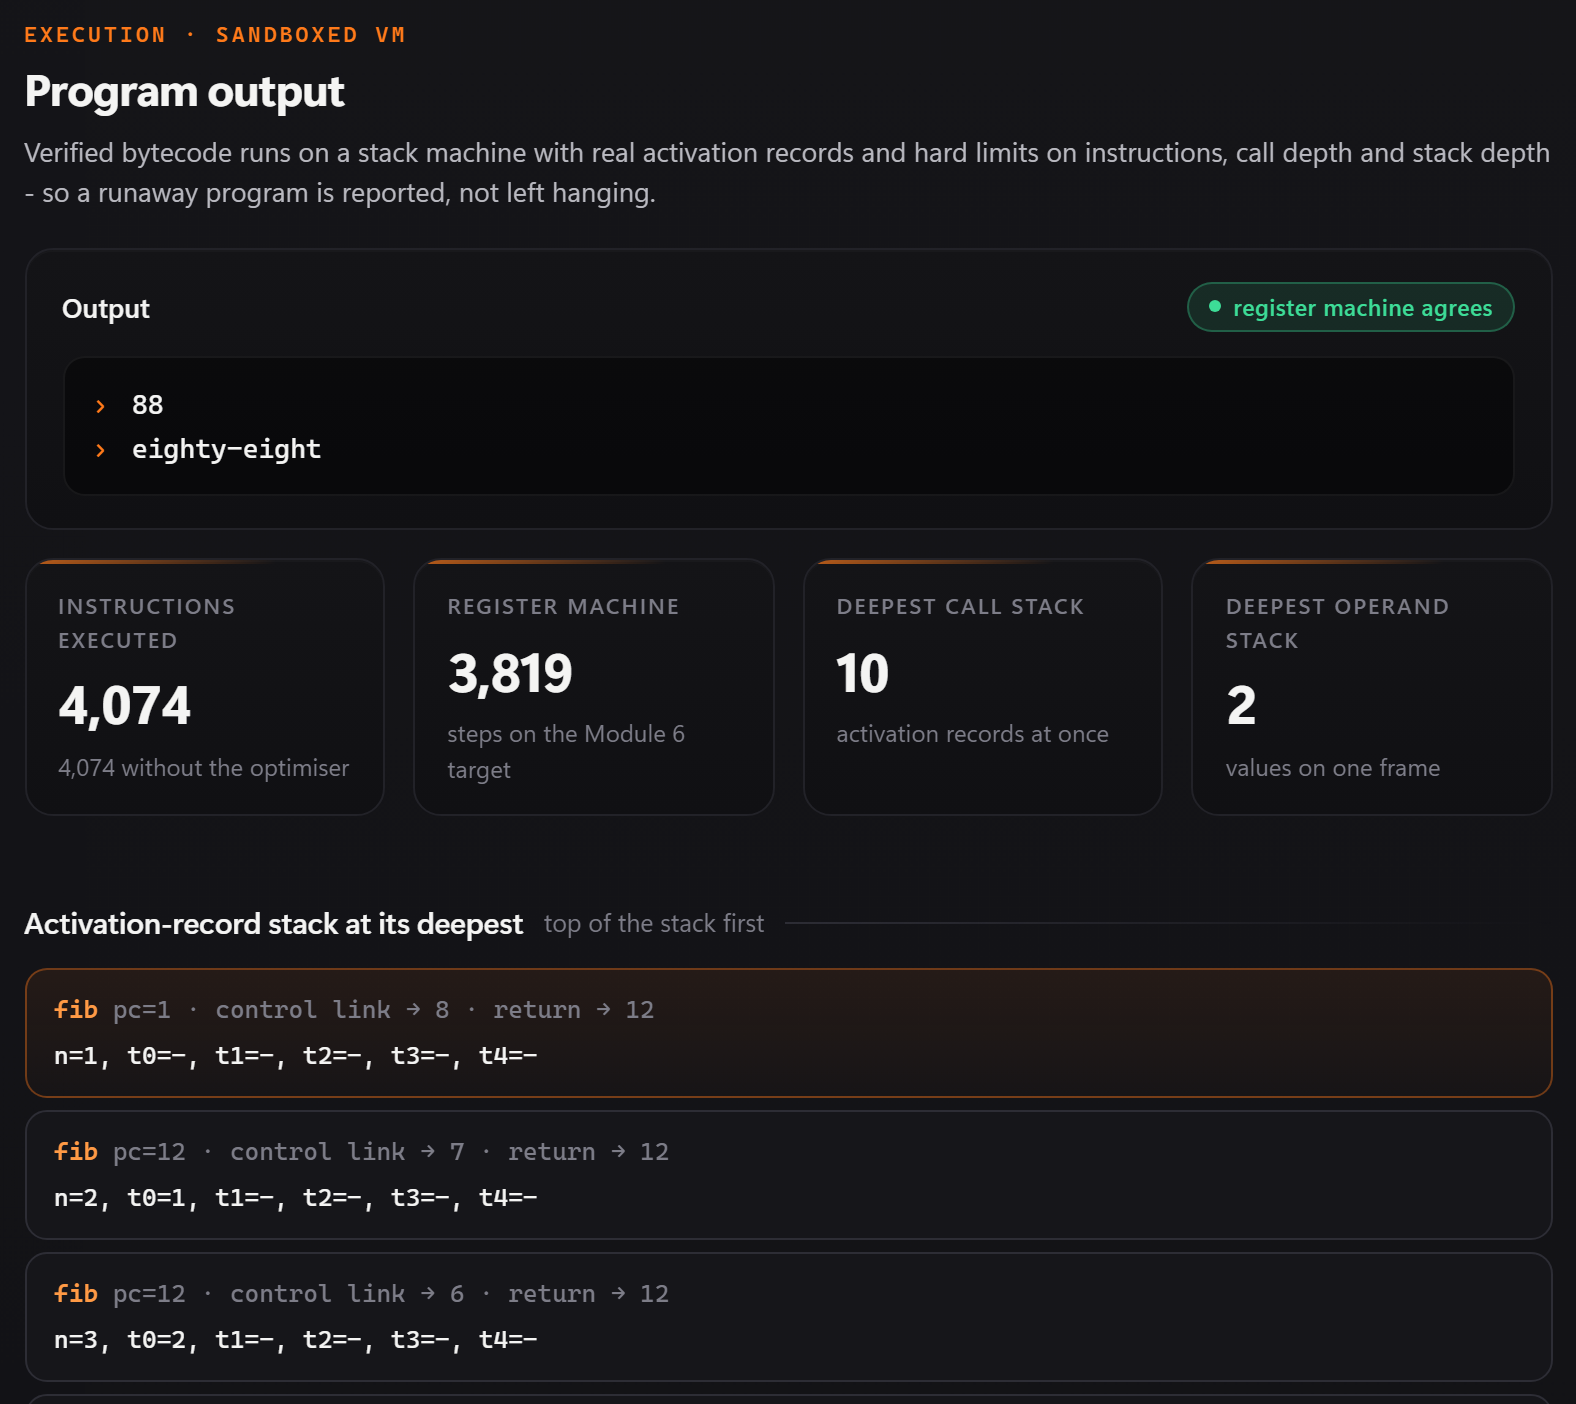
\includegraphics[width=0.96\columnwidth]{figures/view-execution.png}
\caption{Execution view for the Fibonacci benchmark: the program output (confirmed by the register machine), instruction counts on both targets, and the activation-record stack at its deepest, top first. Each frame shows its function, program counter, control link, return address and the current values of its locals.}
\label{fig:execution}
\end{figure}

\begin{figure}[!t]
\centering
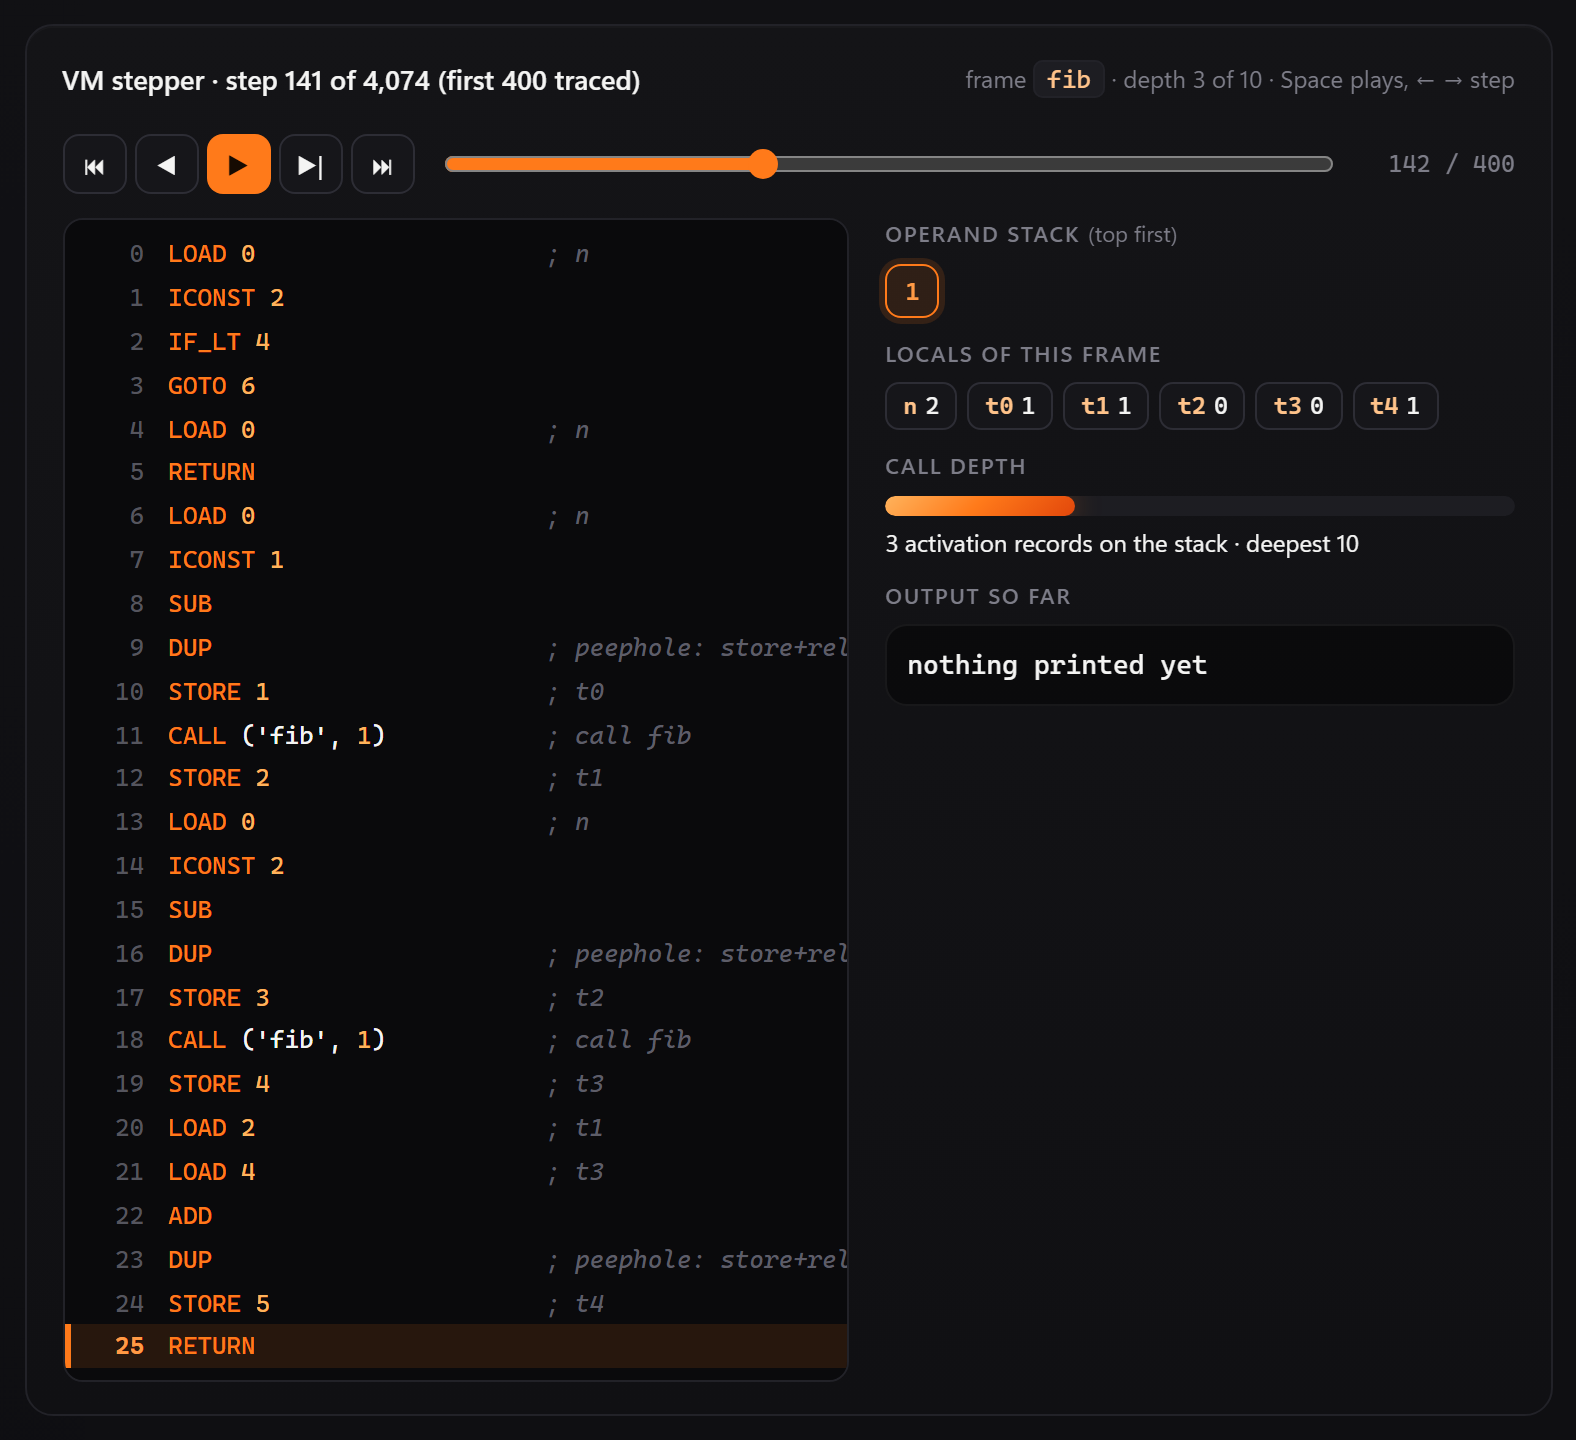
\includegraphics[width=\columnwidth]{figures/vm-stepper.png}
\caption{The VM stepper at step 141 of the Fibonacci run, three frames deep inside \code{fib}: the program counter sits on \code{RETURN}, the operand stack holds the value \code{1} about to be returned, the locals show \code{n=2} and the two partial results \code{t0} and \code{t4}, and nothing has been printed yet.}
\label{fig:stepper}
\end{figure}

\begin{figure*}[!t]
\centering
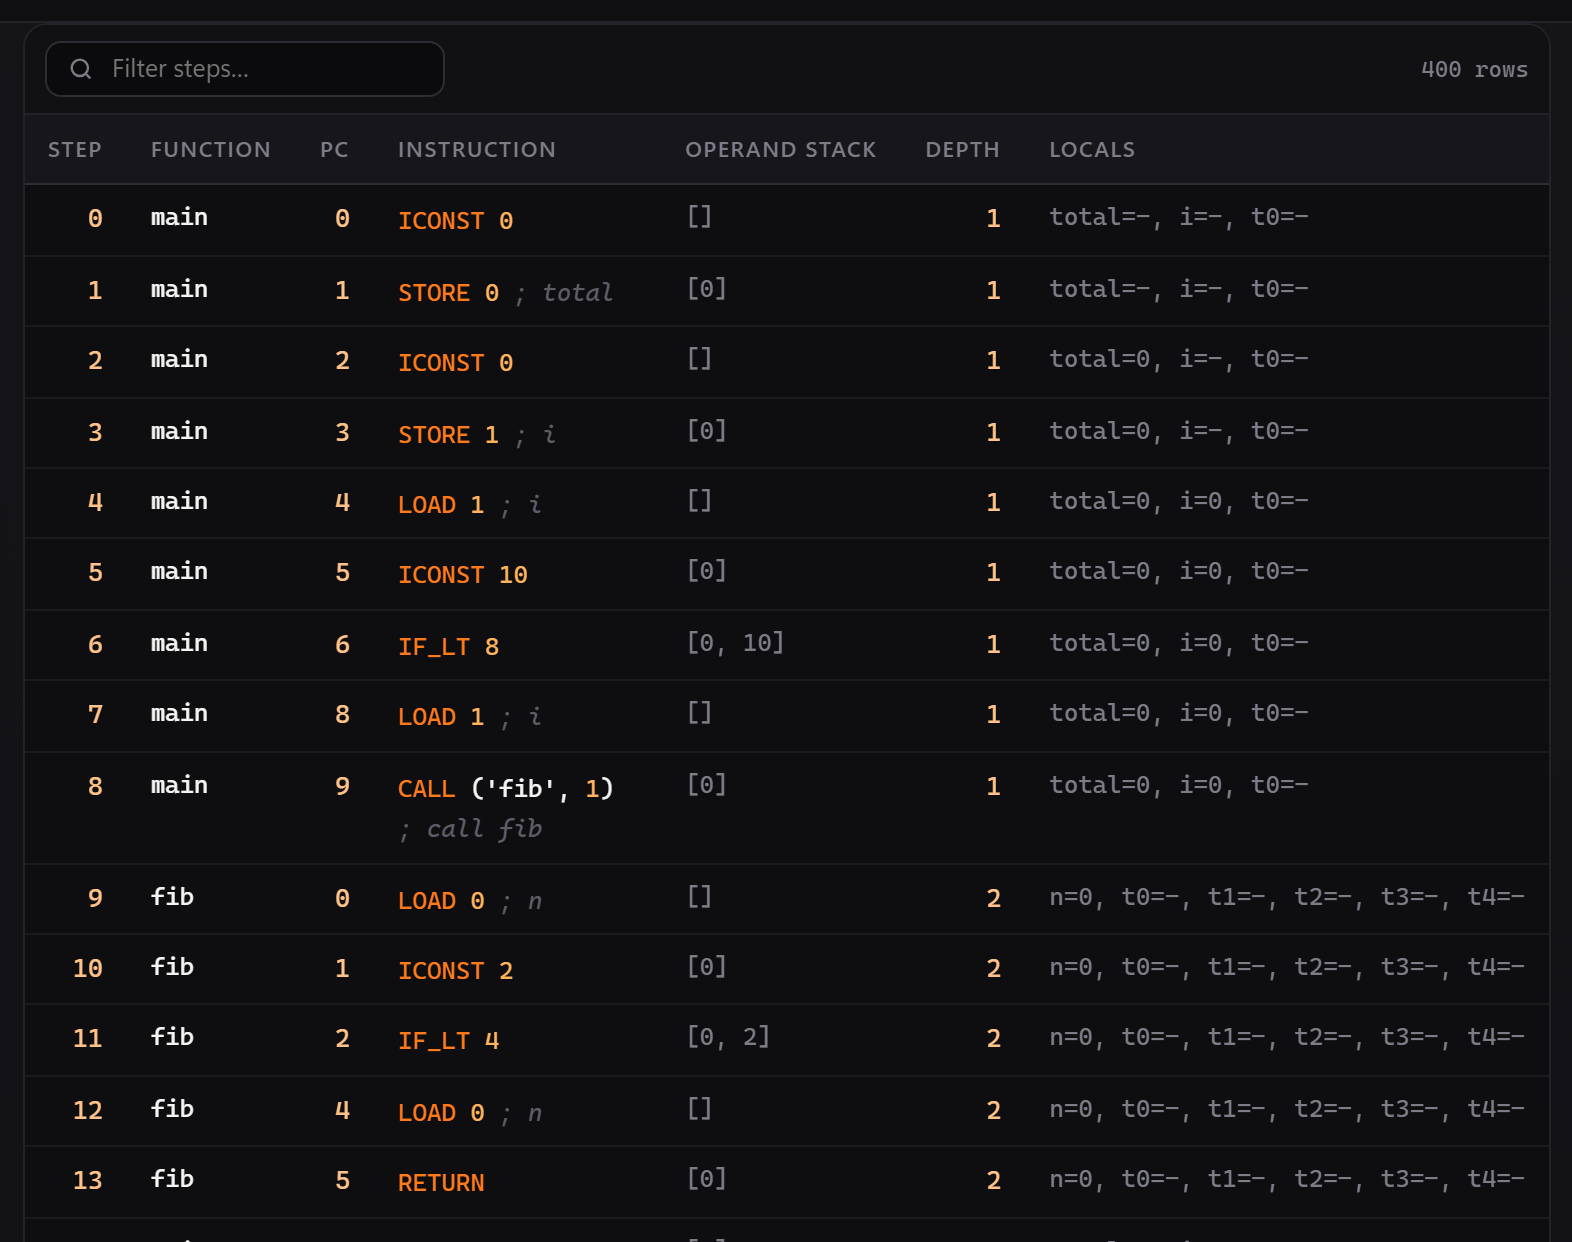
\includegraphics[width=0.8\textwidth]{figures/vm-trace.png}
\caption{The first fourteen rows of the execution trace of the Fibonacci program, with the operand stack, the call depth and the locals of the current frame at every step. Step 8 is the first \code{CALL}; step 9 begins inside \code{fib} with \code{n=0}.}
\label{fig:vmtrace}
\end{figure*}

\begin{figure}[!t]
\centering
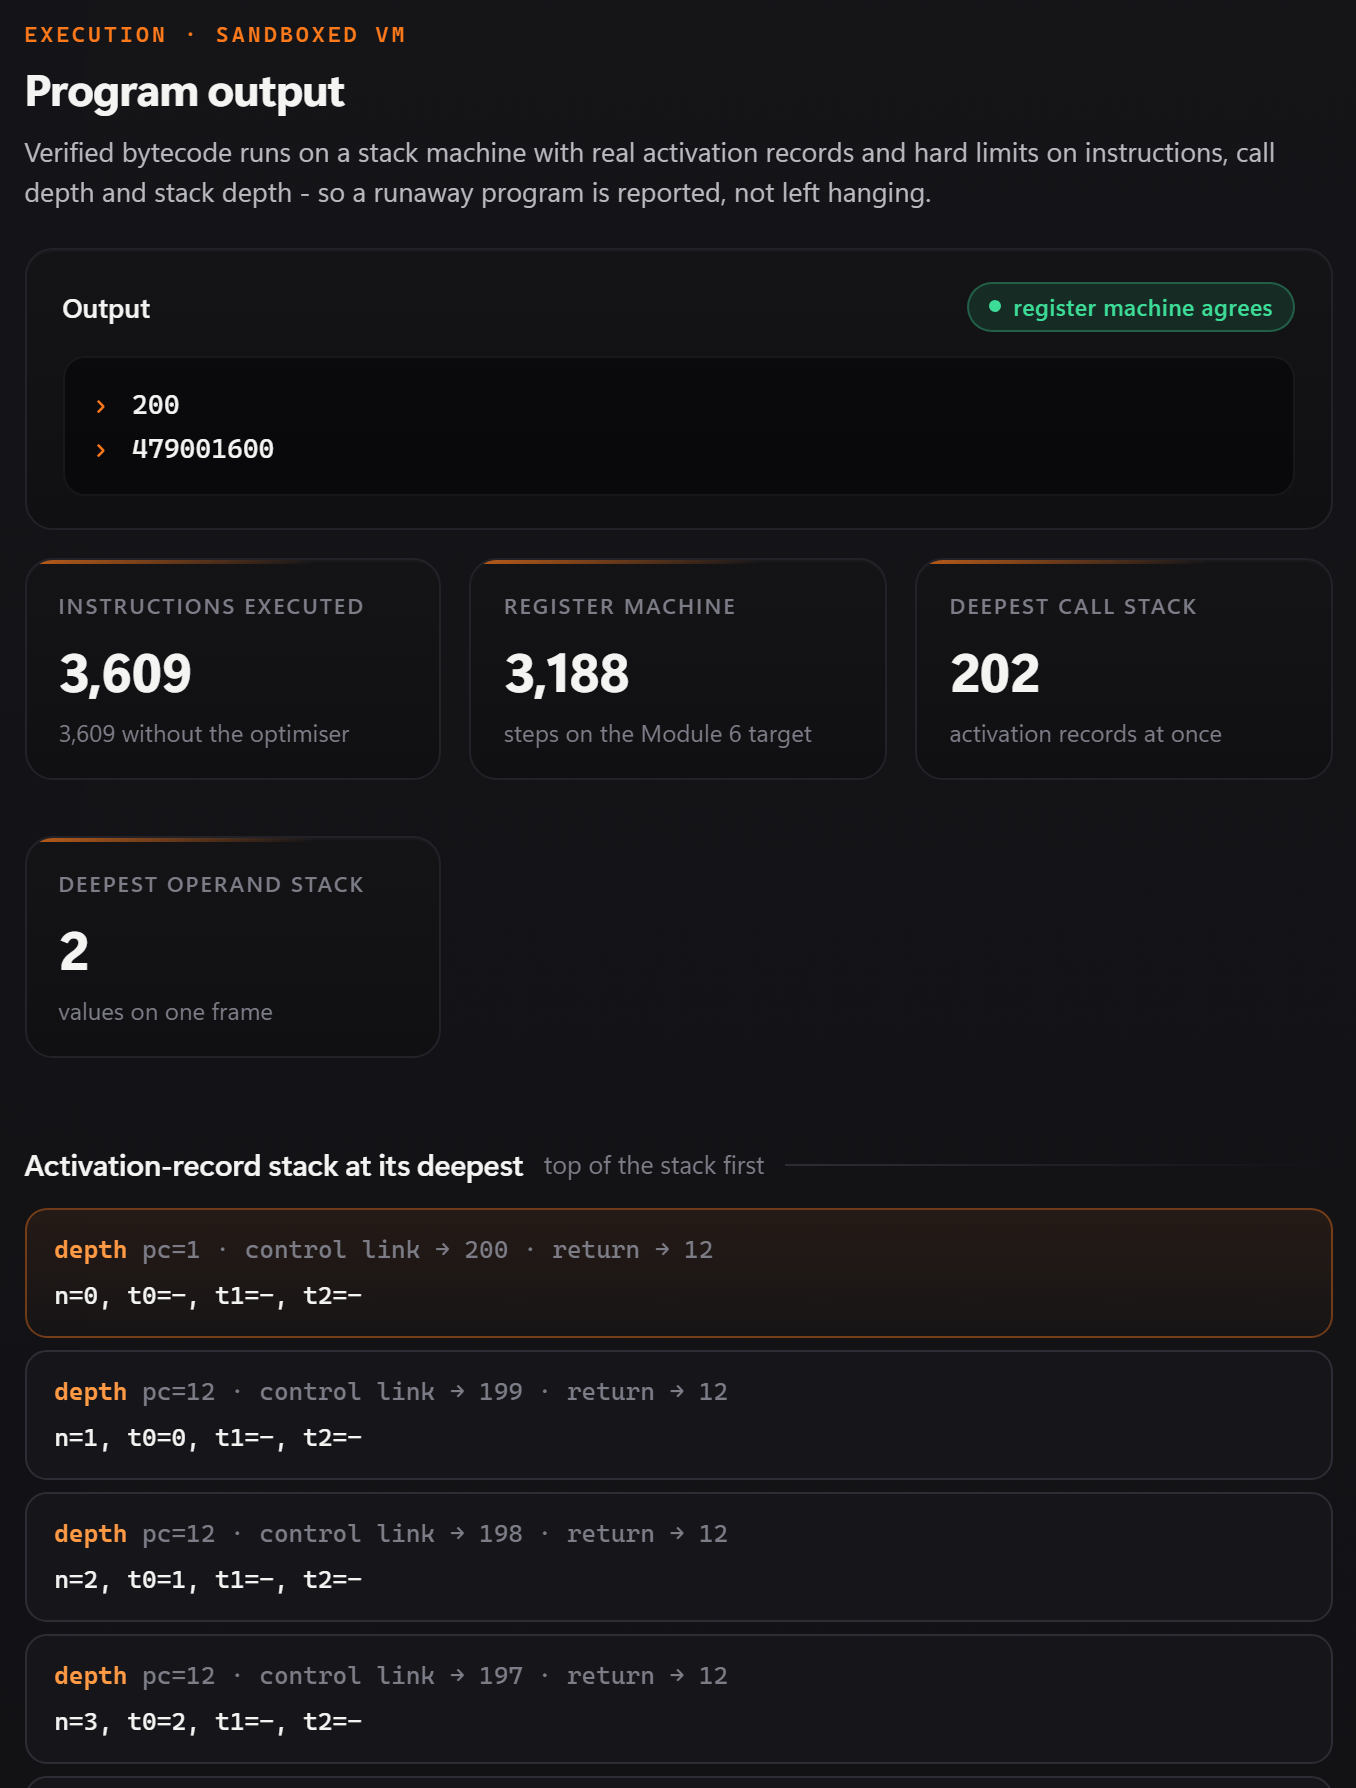
\includegraphics[width=\columnwidth]{figures/deep-recursion.png}
\caption{\code{11\_deep\_recursion.nova}: 202 activation records at the deepest point---\code{main}, then 200 frames of \code{depth} and the frame that returns 0---each with its control link to the frame below, inside the sandbox's limit of 256. Changing \code{200} to \code{300} makes the sandbox stop the program instead.}
\label{fig:deeprec}
\end{figure}

\begin{figure*}[!t]
\centering
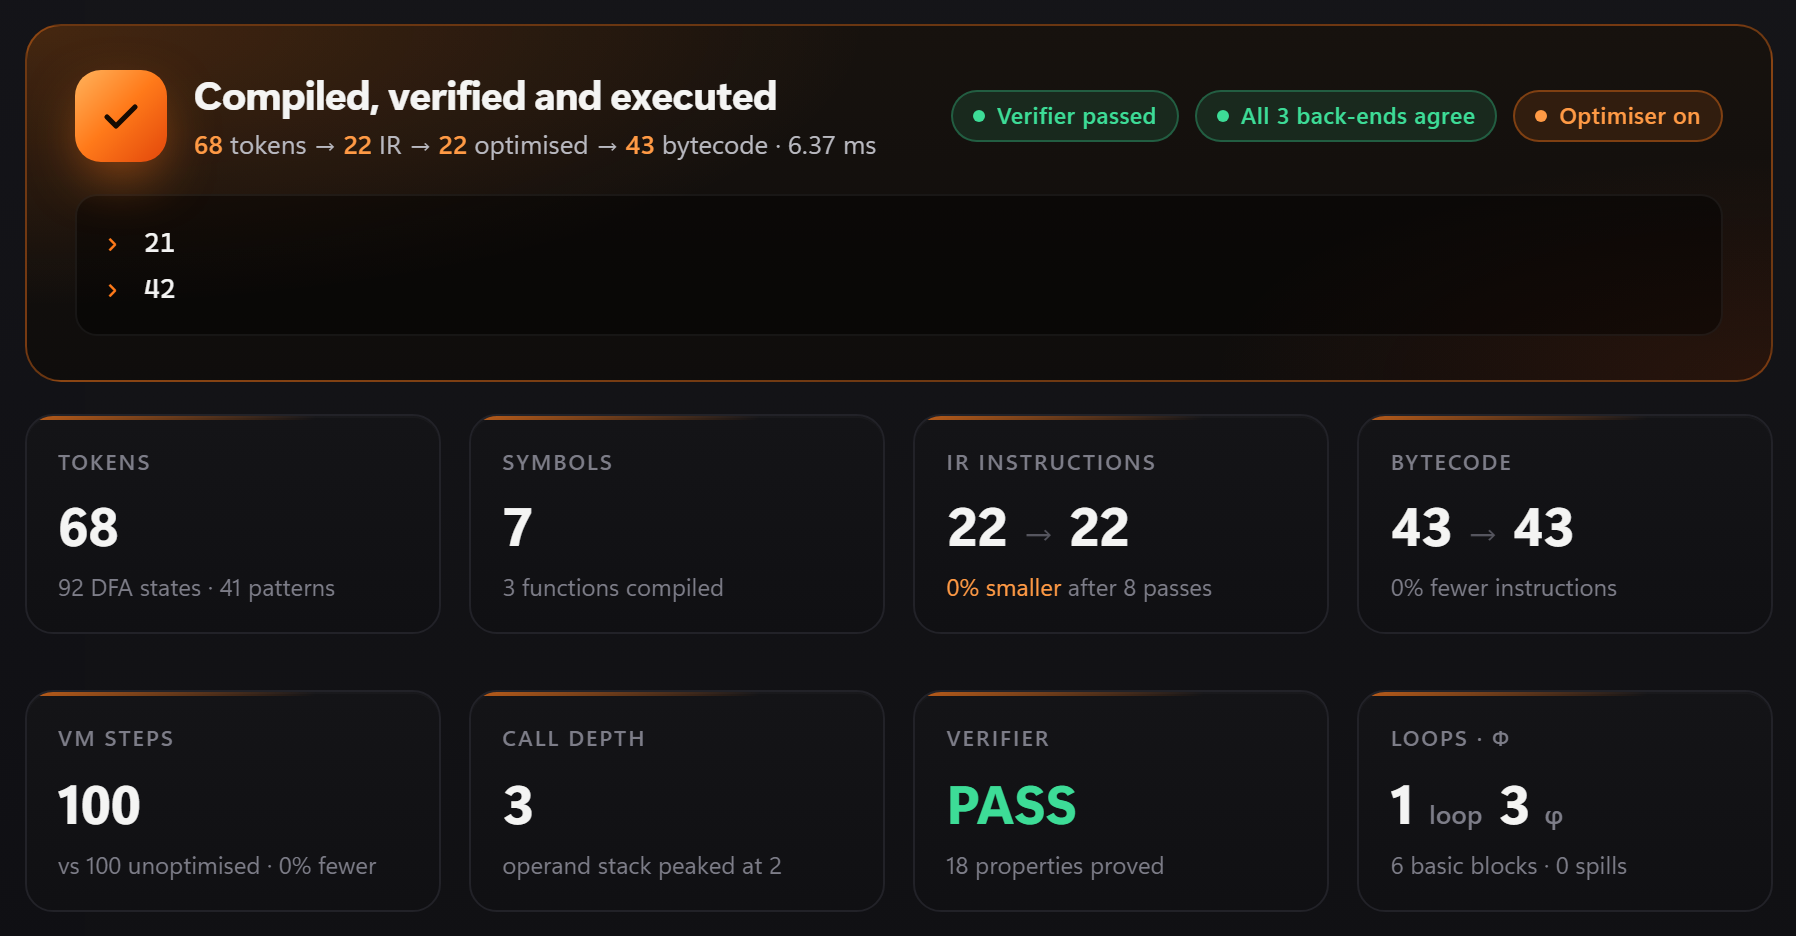
\includegraphics[width=0.8\textwidth]{figures/overview-gcd.png}
\caption{The overview of \code{03\_gcd.nova}: 68 tokens, 22 IR instructions (no redundancy to remove), 43 bytecode instructions, 100 VM steps, a call depth of three, eighteen properties proved and one loop with three $\phi$-functions---the ones restored by the fix to defect D6.}
\label{fig:gcdoverview}
\end{figure*}

\subsection{SSA and Parallelism}
The suite contains eleven natural loops. The dependence analyser classifies two as vectorisable (in \code{isprime} and the first loop of \code{parallel}), six as reductions (the accumulators \code{total}, \code{sum}, \code{acc} and \code{b}, and both loops of \code{nested}, which accumulate \code{total}) and three as sequential (\code{gcd}'s Euclidean step, the recurrence on \code{c} in \code{parallel} and the countdown on \code{n} in \code{types}). Each verdict matches a manual analysis of the loop, and Fig.~\ref{fig:loops} shows how three syntactically similar loops in \code{parallel} receive three different verdicts---the distinction a vectoriser must make before transforming anything~\cite{allen2001}. For the nested pair (Fig.~\ref{fig:nested}) the analyser additionally reports the nesting depth and recommends interchange and tiling, the two transformations Kennedy and McKinley~\cite{kennedy1993} use to improve locality. The 39 $\phi$-functions follow the iterated dominance frontiers exactly; the dominator tree of \code{isprime} (Fig.~\ref{fig:domtree}) shows the frontier $\{\code{B4}\}$ on every block that can re-enter the loop header, which is where its nine $\phi$-functions go. For \code{gcd}, whose loop header is its entry block, Fig.~\ref{fig:ssa} shows the $\phi$-functions that a defect previously suppressed (Section~\ref{sec:res-defects}).

\subsection{Verification and Security}
\label{sec:res-security}
All 114 property checks on the honest programs pass (Fig.~\ref{fig:verifier}), and verification is cheap: 0.054--0.480\,ms per program, under 3\% of compile time. Table~\ref{tab:attacks} reports the hostile suite, which reuses the same verifier and VM with tighter run-time limits of 200,000 instructions and 64 frames. All eight attacks are stopped. Six are memory- or type-safety violations that the verifier rejects before execution, each named by the property it violates (Fig.~\ref{fig:security}). The last two are well typed and therefore pass verification; they are denials of service, which no static check can decide in general, and the sandbox stops them at run time (Fig.~\ref{fig:sandbox}). The middle of the suite (Fig.~\ref{fig:secmiddle}) shows two attacks that a naive stack machine would execute silently: multiplying a string by an integer, and reading a local slot that was never written. This is the division of labour between validation and resource limits that WebAssembly and eBPF also adopt~\cite{haas2017,gershuni2019}.

\begin{table}[!t]
\caption{Hostile Bytecode Suite}
\label{tab:attacks}
\centering
\footnotesize
\setlength{\tabcolsep}{3pt}
\begin{tabular}{@{}r L{3.2cm} l l@{}}
\toprule
\# & Attack & Violates & Stopped by \\
\midrule
1 & Branch outside the code & P3 & verifier \\
2 & Operand-stack underflow & P1/P2 & verifier \\
3 & Inconsistent depth at a merge & P1 & verifier \\
4 & Type confusion (string $\times$ int) & P2 & verifier \\
5 & Read of an uninitialised local & P4 & verifier \\
6 & Slot outside the activation record & P5 & verifier \\
7 & Non-terminating loop & budget & sandbox \\
8 & Unbounded recursion & frame limit & sandbox \\
\bottomrule
\end{tabular}
\end{table}

\begin{figure}[!t]
\centering
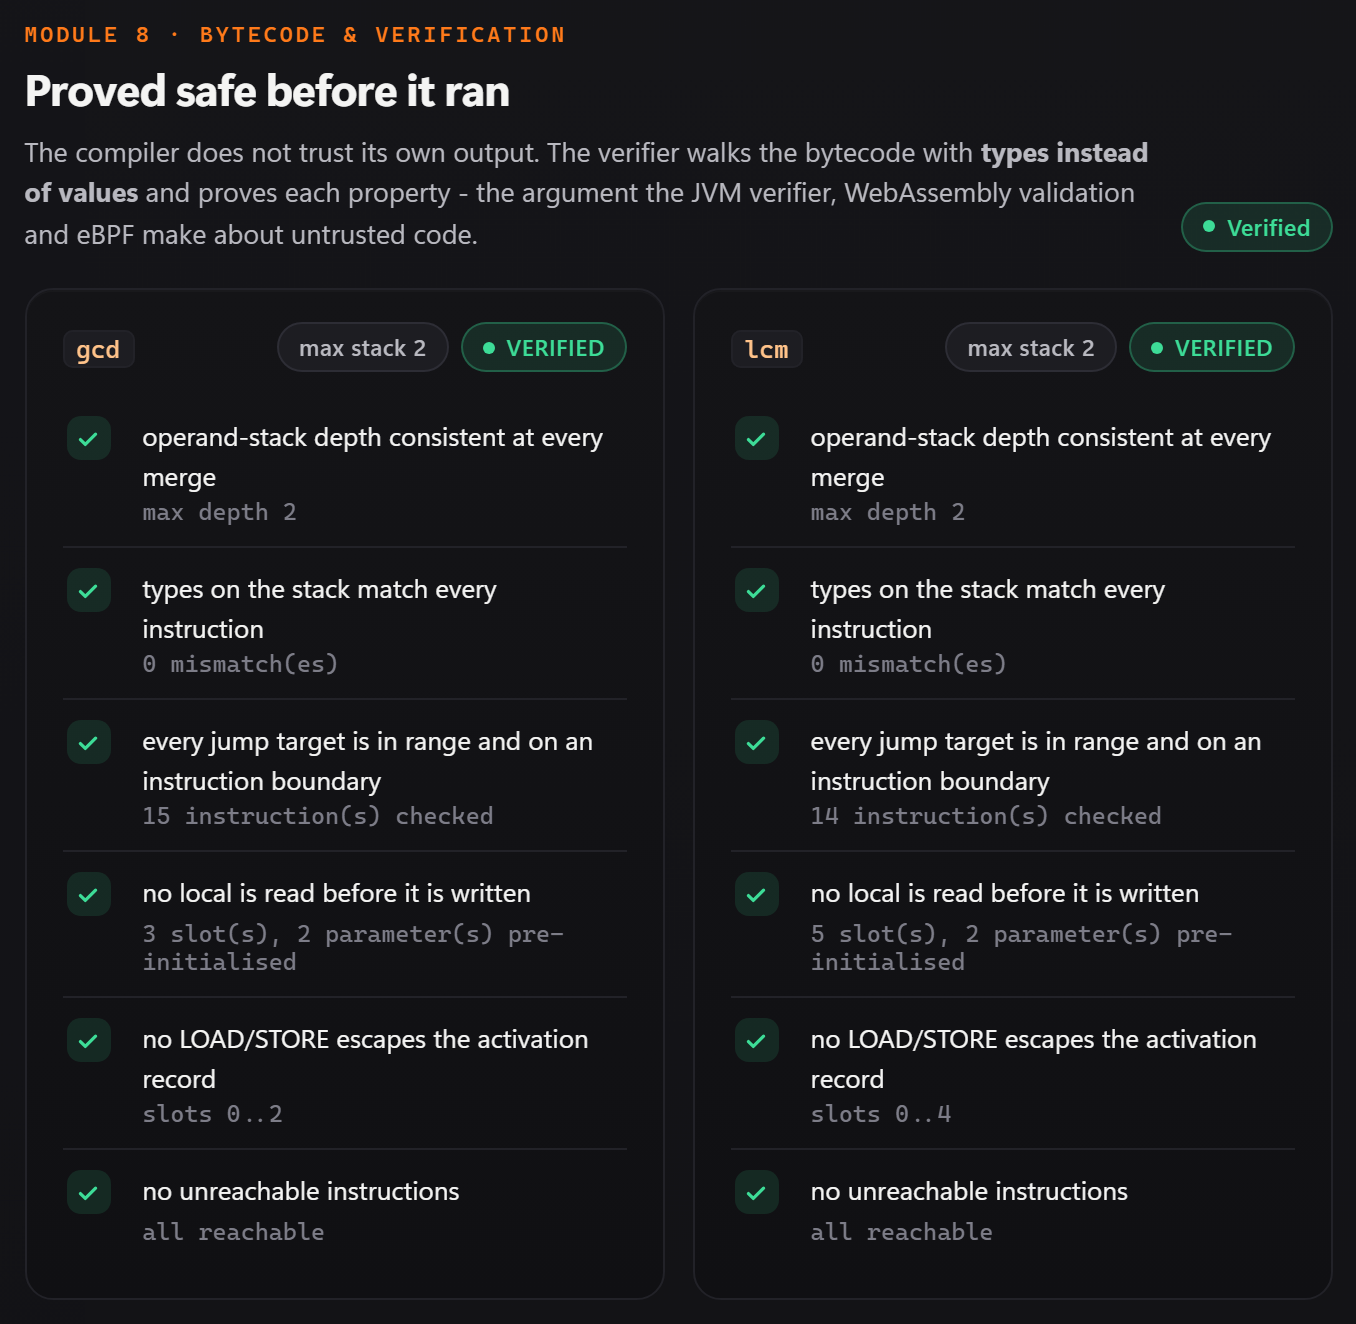
\includegraphics[width=0.92\columnwidth]{figures/view-verifier.png}
\caption{Verifier view for \code{gcd} and \code{lcm}: six properties proved for each function before execution, with the evidence for each, such as the maximum stack depth, the number of jump targets checked and the slots that are pre-initialised.}
\label{fig:verifier}
\end{figure}

\begin{figure}[!t]
\centering
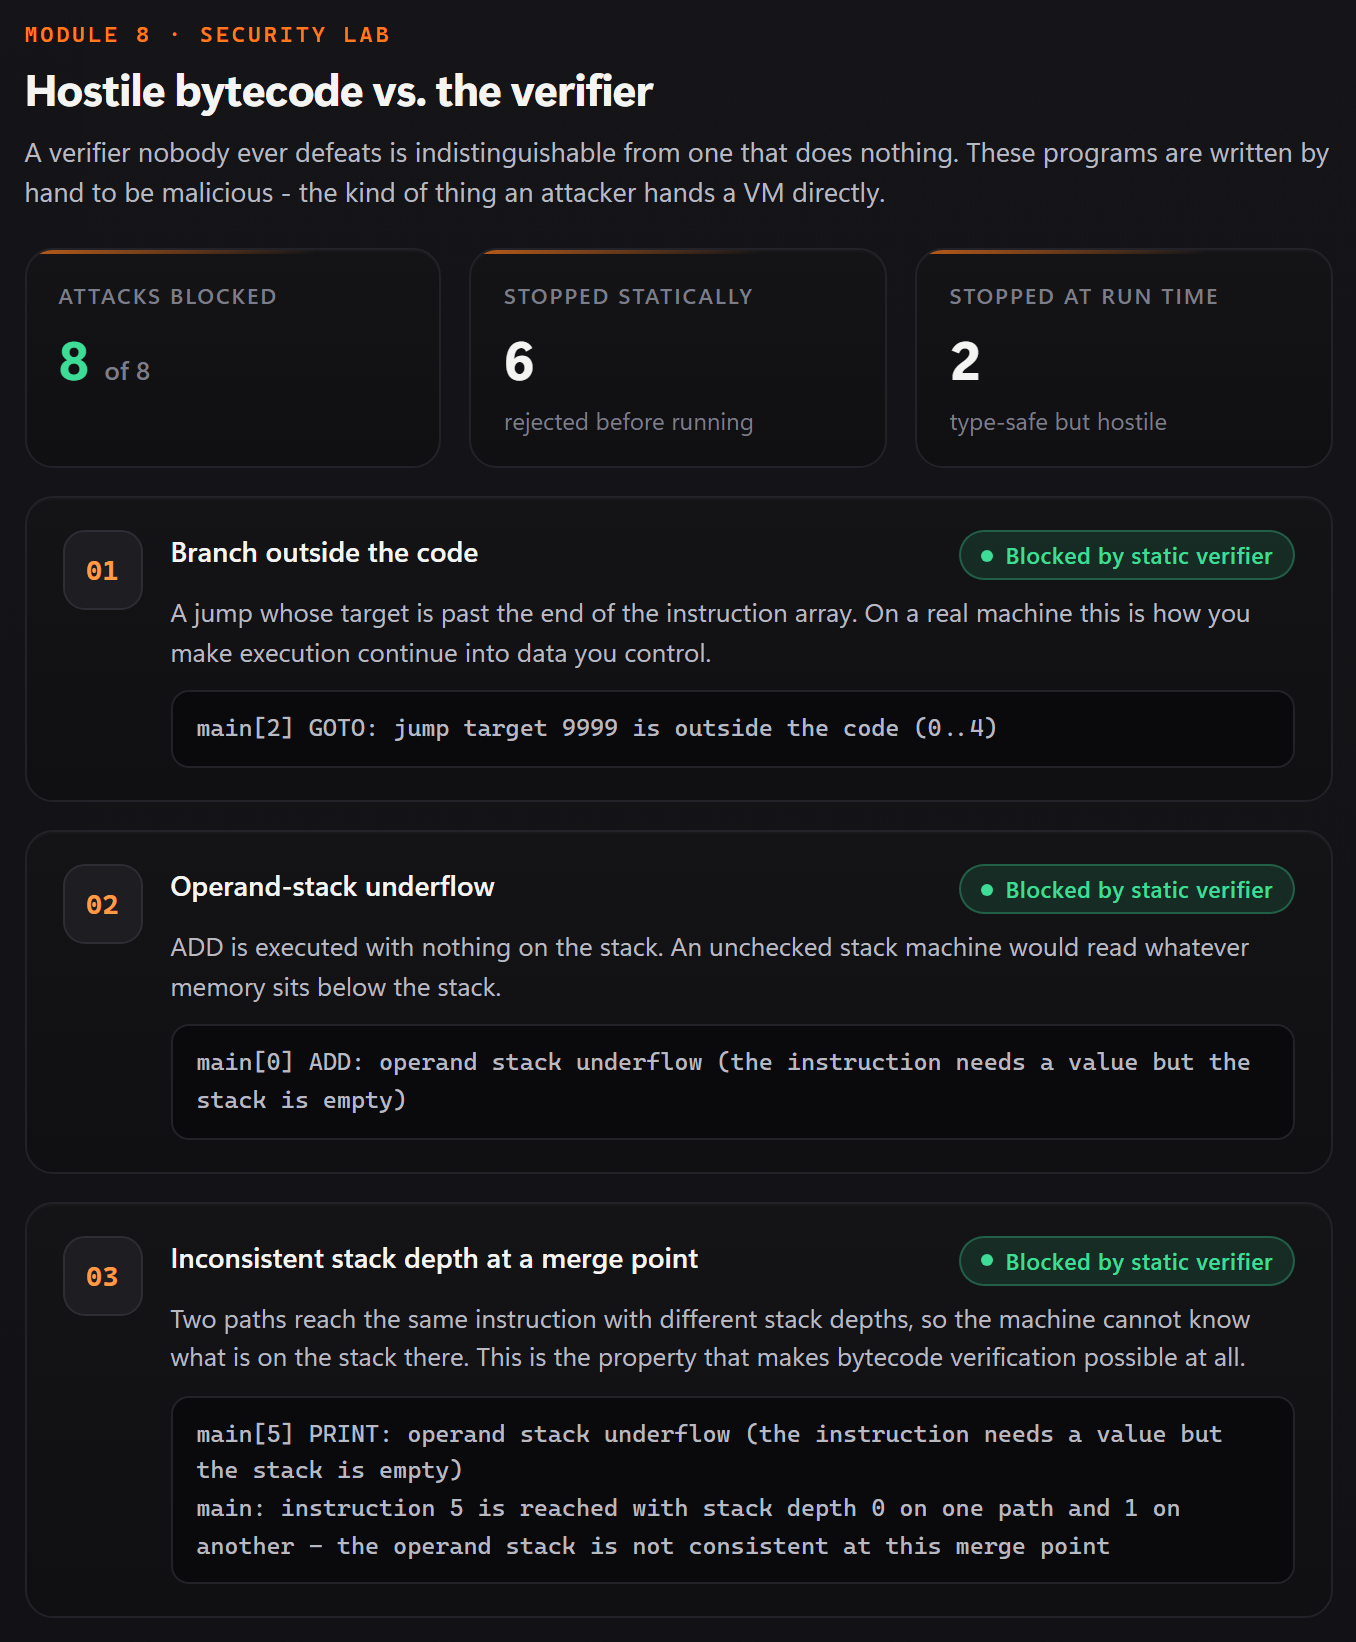
\includegraphics[width=0.92\columnwidth]{figures/view-security.png}
\caption{Security lab: eight hostile programs handed directly to the VM, eight blocked---six statically, two at run time. The first three are shown, each with the property violated and the verifier's exact message.}
\label{fig:security}
\end{figure}

\begin{figure}[!t]
\centering
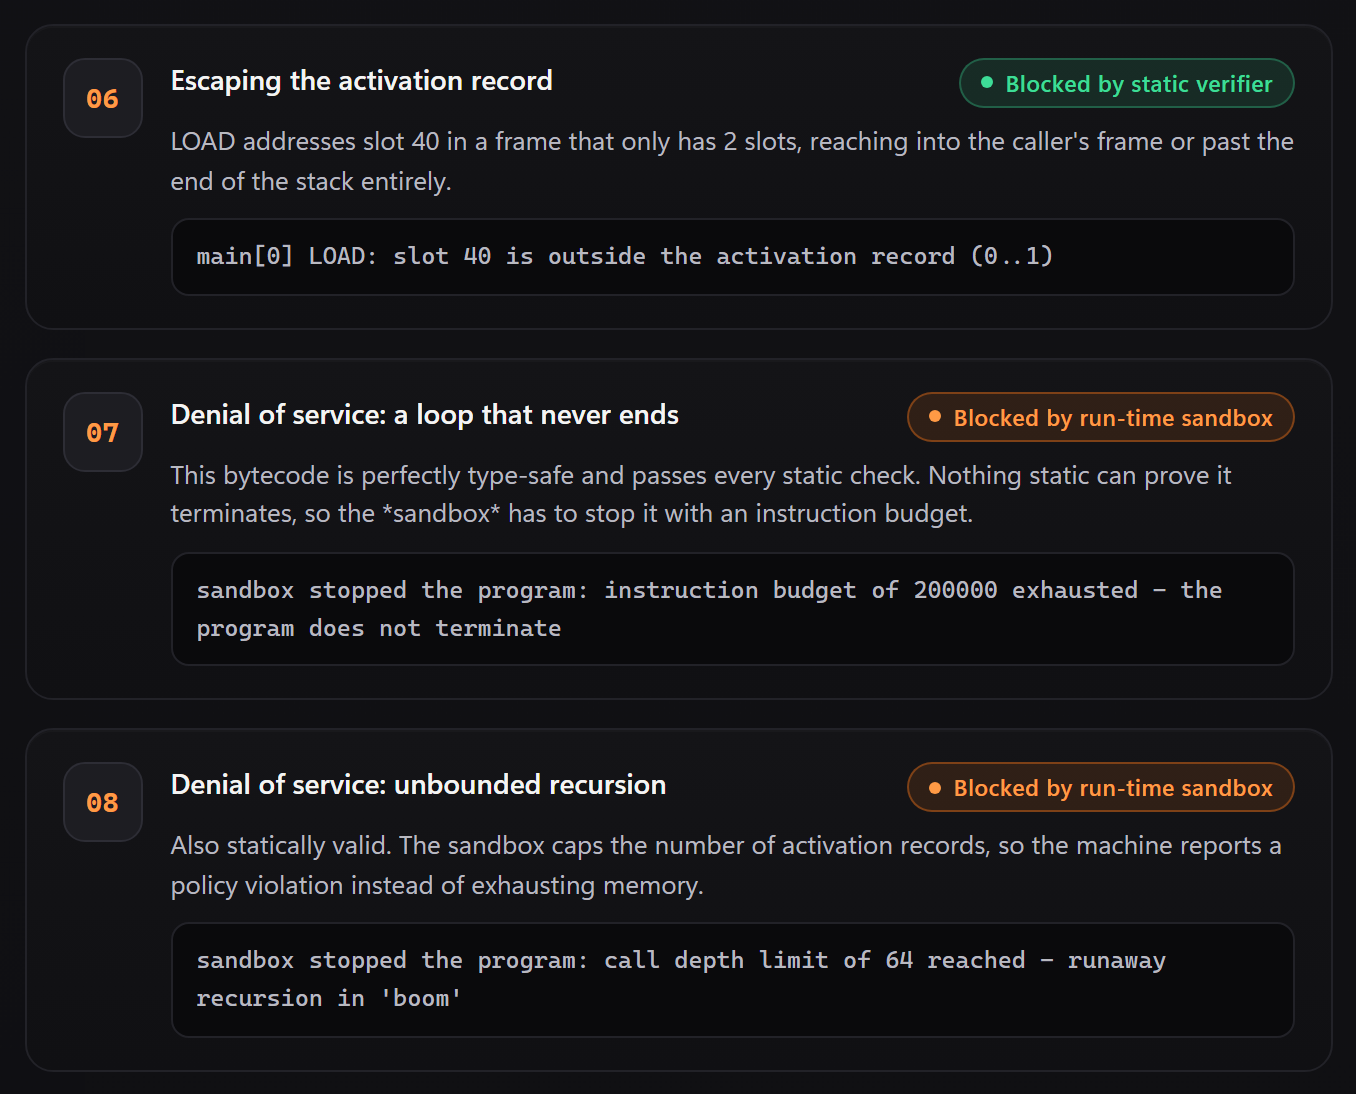
\includegraphics[width=0.92\columnwidth]{figures/security-sandbox.png}
\caption{The last three attacks. The frame-escaping \code{LOAD} is rejected statically; the non-terminating loop and the unbounded recursion pass every static check and are stopped by the sandbox's instruction budget and frame limit.}
\label{fig:sandbox}
\end{figure}

\begin{figure}[!t]
\centering
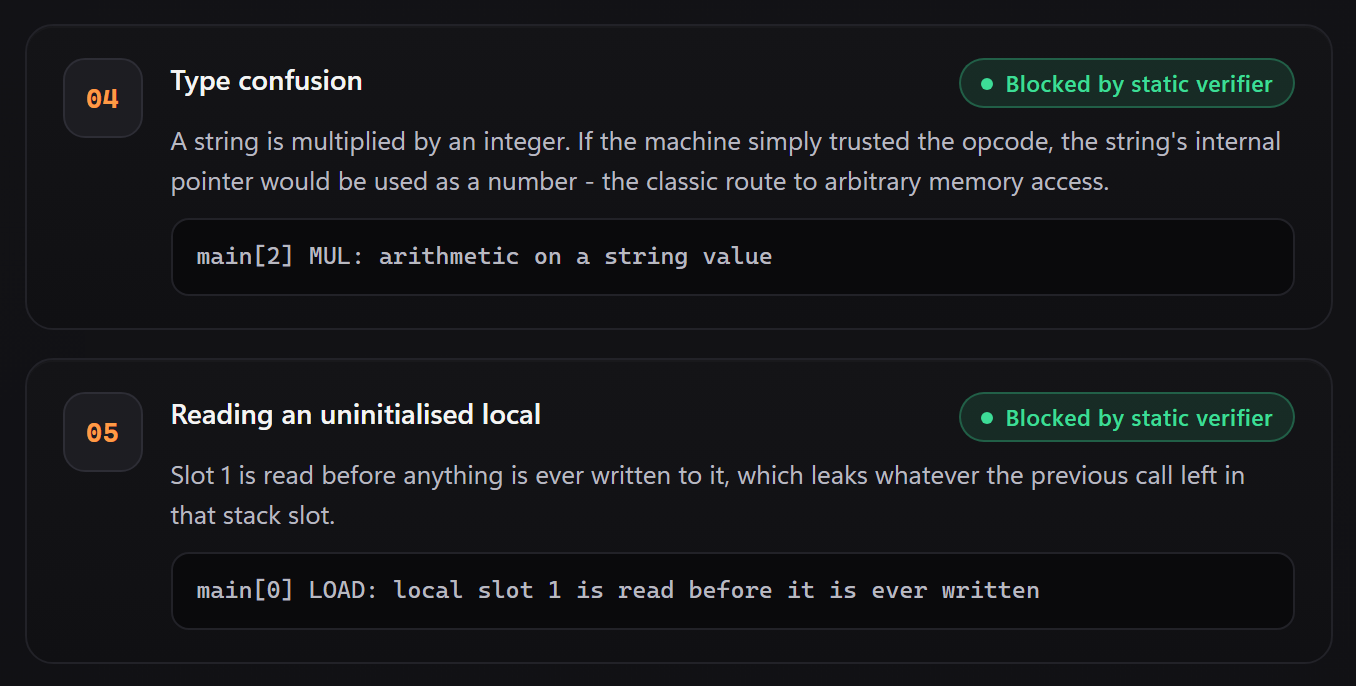
\includegraphics[width=0.85\columnwidth]{figures/security-middle.png}
\caption{Attacks 4 and 5: type confusion (a string multiplied by an integer, rejected by property P2) and the read of an uninitialised local (rejected by definite-assignment property P4).}
\label{fig:secmiddle}
\end{figure}

\subsection{Diagnostics and Robustness}
On \code{broken}, the front end reports seven diagnostics in one run: one lexical error, two syntax errors, two semantic errors and two warnings, each with its line and column and a hint (Fig.~\ref{fig:diagnostics}). Panic-mode recovery and the poisoned error type prevent cascades: every error in the program is reported once, and no spurious errors are added.

\begin{figure*}[!t]
\centering
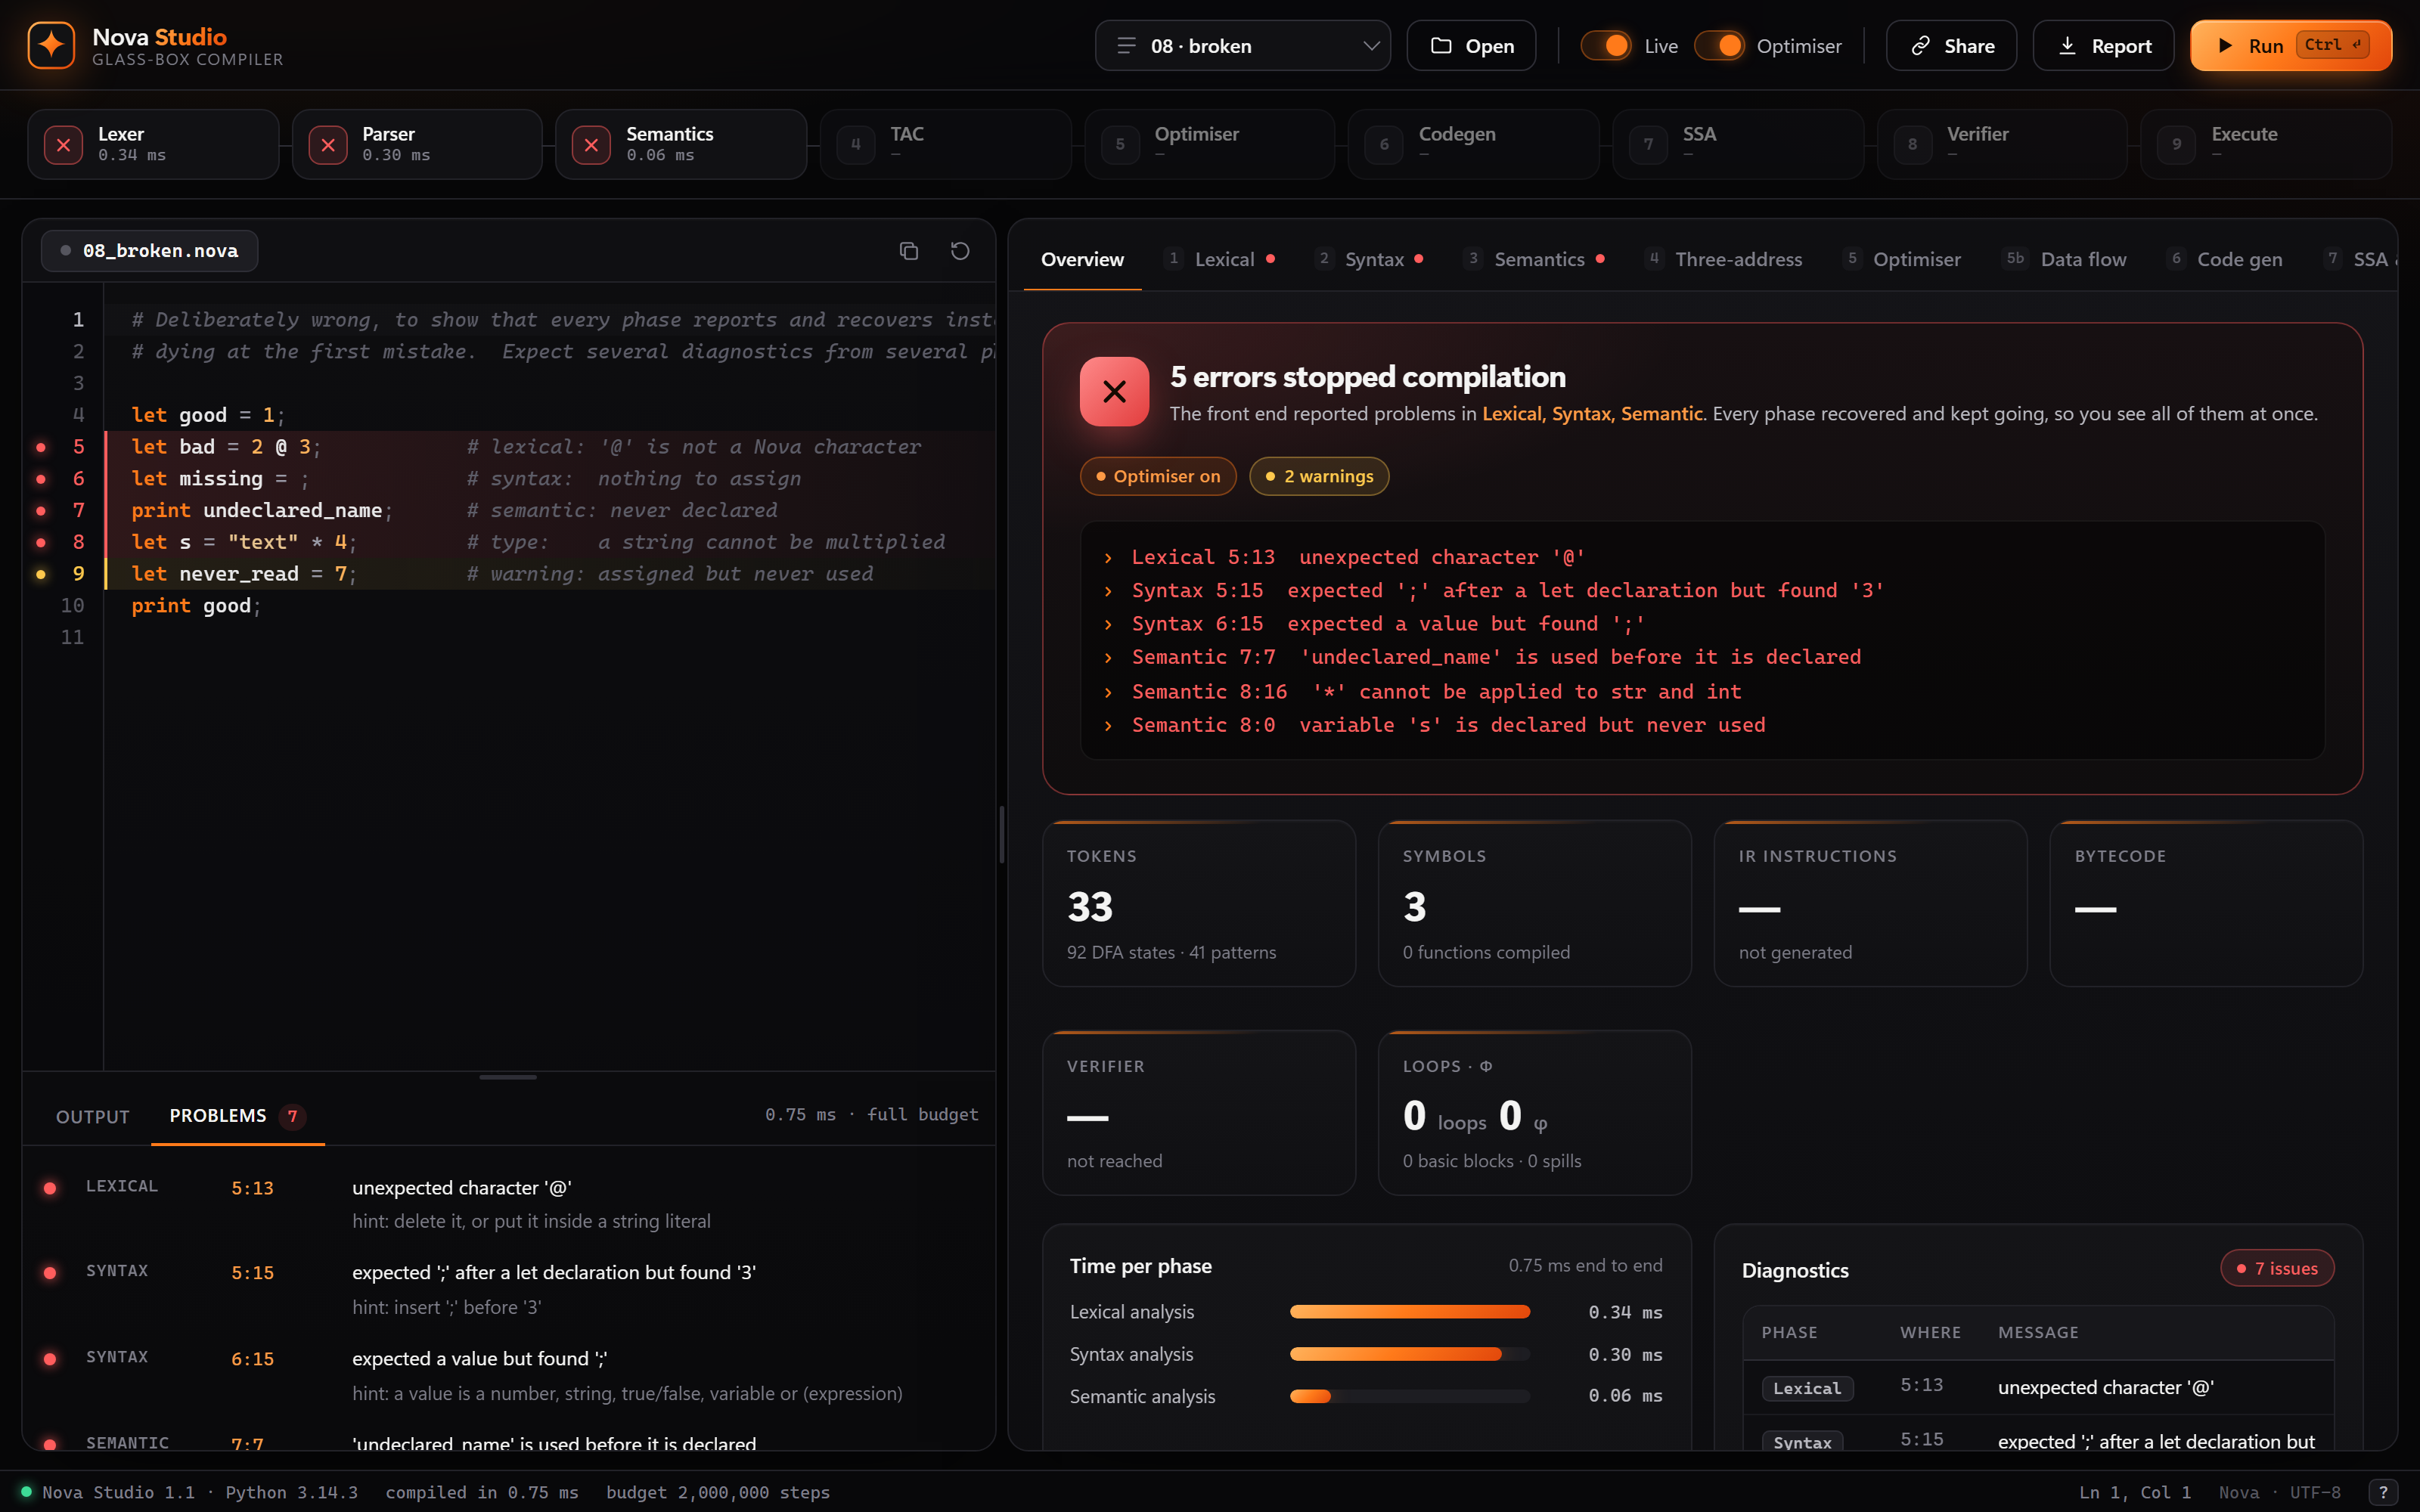
\includegraphics[width=0.95\textwidth]{figures/studio-diagnostics.png}
\caption{Error recovery in Nova Studio on \code{08\_broken.nova}. The rail shows the lexer, parser and semantic analyser failing and later stages skipped. The gutter marks the four lines with errors in red and the line with only a warning in amber. The problems panel lists all seven diagnostics with hints, and each entry jumps to its line when clicked.}
\label{fig:diagnostics}
\end{figure*}

The studio was also probed with inputs designed to break it. A program with 3,000 nested parentheses previously crashed the compiler with a Python recursion error; it now yields a syntax diagnostic in 20.7\,ms. Unbounded recursion is stopped at 256 frames. A non-terminating loop is stopped after 1.09\,s under the live budget, against 8.75\,s under the full one, and the studio tells the user which budget applied (Fig.~\ref{fig:budget}). This eight-fold faster feedback is what makes live recompilation safe.

\begin{figure}[!t]
\centering
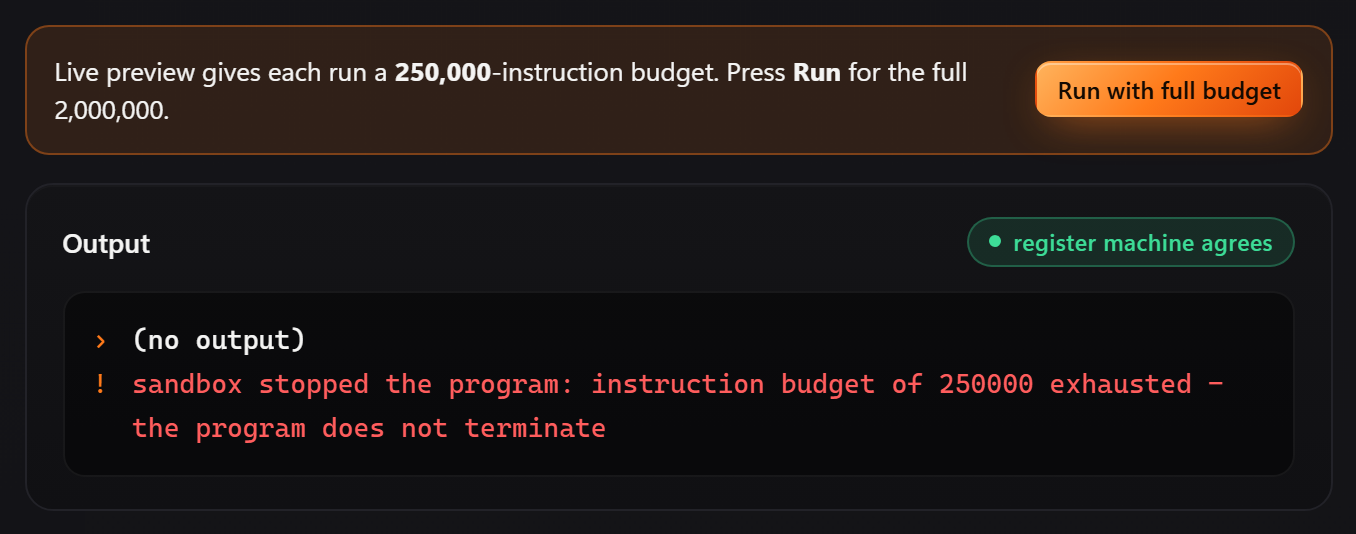
\includegraphics[width=\columnwidth]{figures/view-budget.png}
\caption{A loop typed without its exit condition, stopped by the 250,000-instruction live budget. The studio explains the budget and offers a one-click run with the full 2,000,000-instruction budget.}
\label{fig:budget}
\end{figure}

\subsection{Performance, Interactivity and Scaling}
\label{sec:res-perf}
Fig.~\ref{fig:timing} breaks the median compile time of each program into phases. A complete compilation---all eight phases, three executions and LLVM emission---takes 1.97--36.3\,ms for nine of the ten valid programs and 0.90\,ms for \code{broken}. Work in modules 5--7 and execution dominate; the front end costs at most 5.5\,ms. For \code{fibonacci}, execution accounts for 77\% of the time, because the program runs three times (11,967 VM instructions in total) and the optimised run records a trace with the locals of every step. Measured from a separate process, as a browser uses it, an HTTP compile request takes 7.4--49.2\,ms end to end for these programs and returns a 26--174\,KB JSON document; a bare health check takes 0.74\,ms, so building, serialising and transferring the full glass-box view adds 5--13\,ms to the compile itself. Including the 360\,ms debounce, an updated view arrives about 0.4\,s after the last keystroke; the debounce, not the compiler, sets the latency, and the phases themselves stay inside the 0.1\,s limit for instantaneous response~\cite{miller1968} for every benchmark except the deep recursion. The page itself is 7.7\,KB of HTML, 52.6\,KB of CSS and 116.8\,KB of JavaScript, plus the 160\,KB grammar document fetched once per session.

\begin{figure}[!t]
\centering
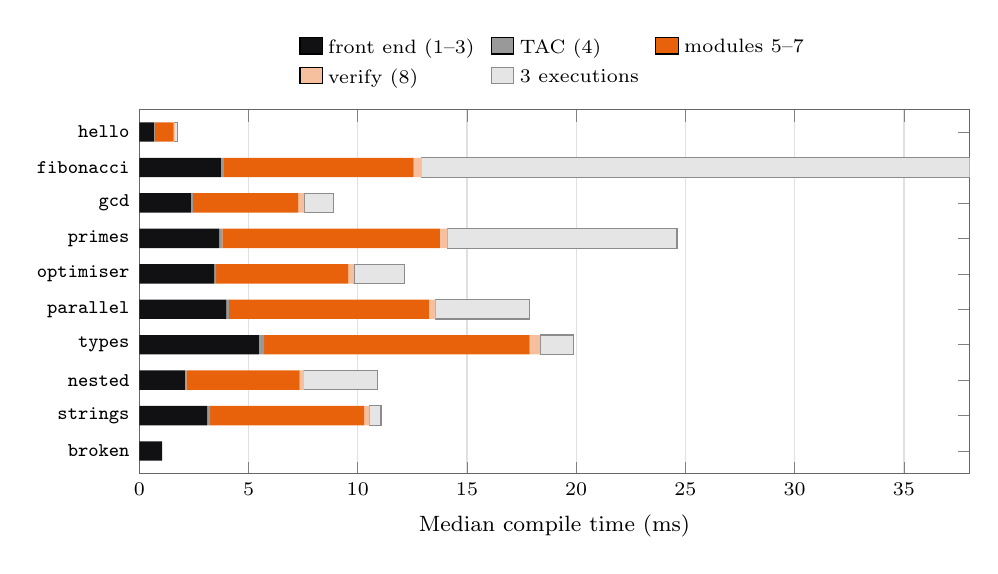
\begin{tikzpicture}
\begin{axis}[
  xbar stacked, width=\columnwidth, height=6.2cm, bar width=7pt,
  xmin=0, xmax=38, xlabel={Median compile time (ms)},
  symbolic y coords={broken,strings,nested,types,parallel,optimiser,primes,gcd,fibonacci,hello},
  ytick=data, yticklabel style={font=\scriptsize\ttfamily},
  tick label style={font=\scriptsize}, label style={font=\footnotesize},
  legend style={font=\scriptsize, draw=none, fill=none, at={(0.5,1.03)}, anchor=south,
    legend columns=3, /tikz/every even column/.append style={column sep=4pt}},
  legend cell align=left, enlarge y limits=0.07, axis line style={black!60},
  xmajorgrids, grid style={black!12}]
\addplot[fill=novablack, draw=none] coordinates {(0.677,hello) (3.739,fibonacci) (2.365,gcd) (3.655,primes) (3.428,optimiser) (3.987,parallel) (5.472,types) (1.043,broken) (2.081,nested) (3.105,strings)};
\addlegendentry{front end (1--3)}
\addplot[fill=black!40, draw=none] coordinates {(0.024,hello) (0.130,fibonacci) (0.082,gcd) (0.149,primes) (0.092,optimiser) (0.110,parallel) (0.242,types) (0,broken) (0.077,nested) (0.135,strings)};
\addlegendentry{TAC (4)}
\addplot[fill=novaorange, draw=none] coordinates {(0.870,hello) (8.690,fibonacci) (4.830,gcd) (9.953,primes) (6.051,optimiser) (9.157,parallel) (12.152,types) (0,broken) (5.184,nested) (7.049,strings)};
\addlegendentry{modules 5--7}
\addplot[fill=novaorange!40, draw=none] coordinates {(0.054,hello) (0.374,fibonacci) (0.266,gcd) (0.350,primes) (0.254,optimiser) (0.307,parallel) (0.480,types) (0,broken) (0.188,nested) (0.251,strings)};
\addlegendentry{verify (8)}
\addplot[fill=black!10, draw=black!45] coordinates {(0.132,hello) (27.984,fibonacci) (1.333,gcd) (10.505,primes) (2.297,optimiser) (4.319,parallel) (1.538,types) (0,broken) (3.368,nested) (0.525,strings)};
\addlegendentry{3 executions}
\end{axis}
\end{tikzpicture}
\caption{Median compile time per benchmark (60 runs, battery power), split into front end, three-address code, modules 5--7 (blocks, data flow, optimisation, register code generation, SSA and dependence analysis, bytecode generation), verification and the three executions. \code{recursion} (194.8\,ms, of which 181.5\,ms is execution) is omitted from the axis. The remaining 0.1--1.3\,ms per program, not drawn, is LLVM IR emission and bookkeeping.}
\label{fig:timing}
\end{figure}

\emph{Scaling.} Table~\ref{tab:scaling} and Fig.~\ref{fig:scaling} report the synthetic series. Compile time grows faster than the program: doubling the program from 56 to 112 lines costs $2.8\times$, from 112 to 224 lines $4.8\times$, and from 224 to 448 lines $7.8\times$, so the growth lies between quadratic and cubic. The front end stays close to linear (16\,ms of lexing and 54\,ms of parsing for 2,112 tokens and 7,299 parse steps at the largest size), and execution and verification are small. Almost all of the growth is in modules 5--7: 4,935 of the 5,297\,ms at 64 loops. The reasons are the glass box's own bookkeeping, which was never designed for large inputs: dominators are computed by iterative intersection of whole sets, which is $O(B^2)$ in the number of blocks $B$; each of the four data-flow analyses copies every block's sets on every round and keeps a snapshot of all of them per round; and the optimiser records the complete code listing after each of its ten passes. These are the costs of keeping everything, and they bound the size of program for which the studio is instantaneous: on this throttled machine, programs of about 60 lines compile within 0.1\,s and programs of about 110 lines within 0.15\,s, while a 448-line program takes 5.3\,s. Section~\ref{sec:conclusion} lists the standard remedies. The JSON document grows with the program as well---57\,KB to 3.7\,MB across the series---but remains bounded by the row caps.

\begin{table}[!t]
\caption{Scaling with Program Size (Synthetic Programs of $N$ Loops)}
\label{tab:scaling}
\centering
\footnotesize
\setlength{\tabcolsep}{3.5pt}
\begin{tabular*}{\columnwidth}{@{\extracolsep{\fill}}r r r r r r r r@{}}
\toprule
$N$ & Lines & Tokens & LR steps & Blocks & IR & ms & JSON KB \\
\midrule
1 & 7 & 33 & 117 & 5 & 10 & 7.8 & 57 \\
2 & 14 & 66 & 231 & 9 & 19 & 10.6 & 98 \\
4 & 28 & 132 & 459 & 17 & 37 & 22.8 & 194 \\
8 & 56 & 264 & 915 & 33 & 73 & 51.1 & 378 \\
16 & 112 & 528 & 1,827 & 65 & 145 & 140.8 & 757 \\
32 & 224 & 1,056 & 3,651 & 129 & 289 & 678.4 & 1,598 \\
64 & 448 & 2,112 & 7,299 & 257 & 577 & 5,296.7 & 3,705 \\
\bottomrule
\end{tabular*}
\end{table}

\begin{figure}[!t]
\centering
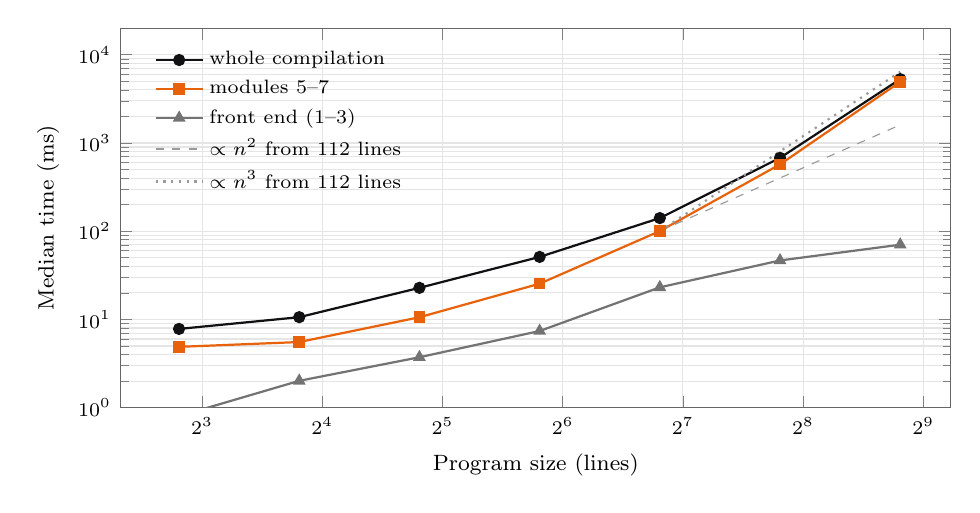
\begin{tikzpicture}
\begin{loglogaxis}[
  width=\columnwidth, height=6.4cm,
  xlabel={Program size (lines)}, ylabel={Median time (ms)},
  xmin=5, xmax=600, ymin=1, ymax=20000,
  tick label style={font=\scriptsize}, label style={font=\footnotesize},
  legend style={font=\scriptsize, draw=none, fill=none, at={(0.03,0.97)}, anchor=north west},
  legend cell align=left, axis line style={black!60},
  grid=both, grid style={black!10}, log basis x=2]
\addplot[novablack, thick, mark=*, mark size=1.8pt] coordinates {(7,7.8) (14,10.6) (28,22.8) (56,51.1) (112,140.8) (224,678.4) (448,5296.7)};
\addlegendentry{whole compilation}
\addplot[novaorange, thick, mark=square*, mark size=1.7pt] coordinates {(7,4.885) (14,5.54) (28,10.582) (56,25.405) (112,100.265) (224,572.085) (448,4935.193)};
\addlegendentry{modules 5--7}
\addplot[black!55, thick, mark=triangle*, mark size=1.9pt] coordinates {(7,0.801) (14,2.013) (28,3.725) (56,7.391) (112,23.102) (224,46.584) (448,70.322)};
\addlegendentry{front end (1--3)}
\addplot[black!40, dashed] coordinates {(112,100.265) (448,1604.24)};
\addlegendentry{$\propto n^{2}$ from 112 lines}
\addplot[black!40, dotted, thick] coordinates {(112,100.265) (448,6416.96)};
\addlegendentry{$\propto n^{3}$ from 112 lines}
\end{loglogaxis}
\end{tikzpicture}
\caption{Compile time against program size on a log--log scale for the synthetic series. The front end grows roughly linearly; modules 5--7 grow between quadratically and cubically, and dominate from about 100 lines upwards.}
\label{fig:scaling}
\end{figure}

\begin{figure}[!t]
\centering
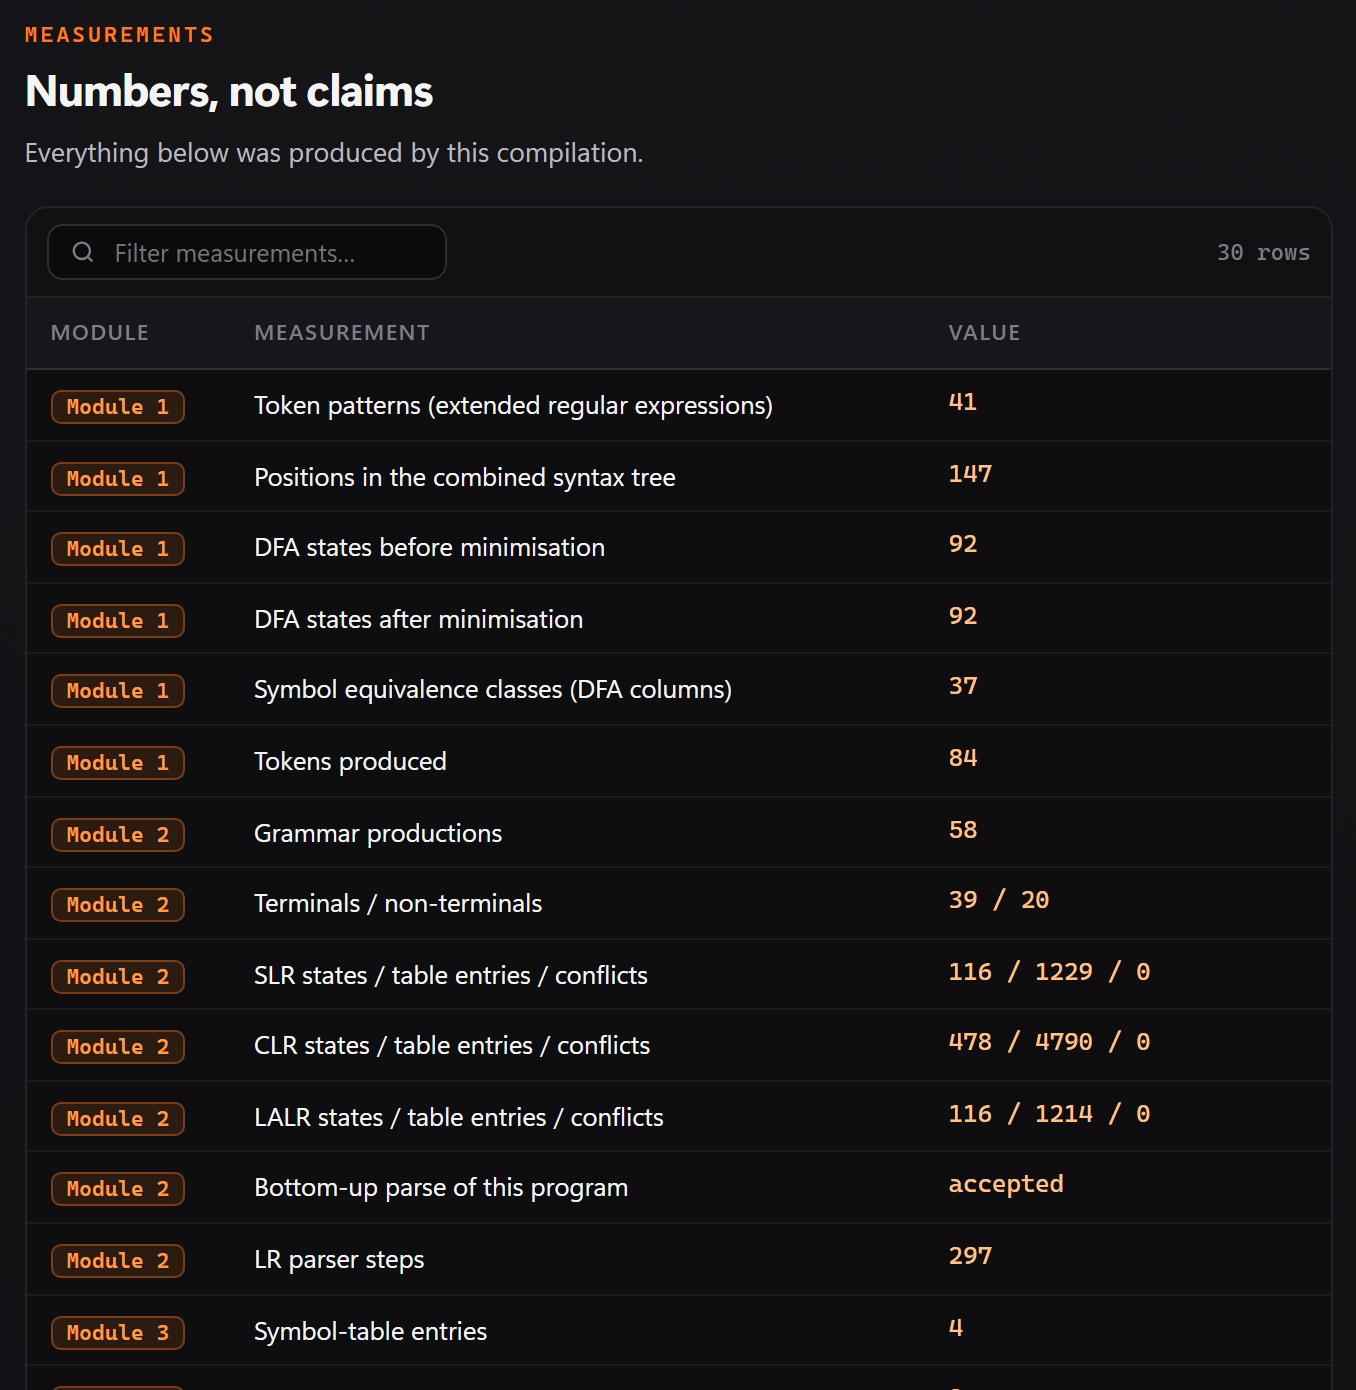
\includegraphics[width=\columnwidth]{figures/view-metrics.png}
\caption{The metrics view: every measurement of the current compilation, produced by the compiler itself, from DFA states and parse-table sizes to verification results and VM step counts.}
\label{fig:metrics}
\end{figure}

\subsection{Defects Exposed by the Glass Box}
\label{sec:res-defects}
Building, measuring and screenshotting every phase exposed six functional defects (Table~\ref{tab:defects}); all are fixed, and five are covered by new regression tests. Two of them are telling. The SSA defect (D6) left \code{gcd} with zero $\phi$-functions---a count that was plainly wrong once it appeared in a measurement table---because the dominance-frontier routine admitted only blocks with two or more recorded predecessors as join points and ignored the implicit edge into the entry block. The symbol-table defect (D5) became visible in a screenshot taken for this report, which showed a function that is called three times as unused. Neither defect affected program output, so output-only testing could never have found them. Both were found because the artefacts were on screen. This is the strongest evidence in this study for the glass-box approach: a tool that shows its working also exposes its own mistakes.

\begin{table*}[!t]
\caption{Defects Exposed While Building and Evaluating Nova Studio}
\label{tab:defects}
\centering
\footnotesize
\setlength{\tabcolsep}{4pt}
\begin{tabular}{@{}l l L{4.1cm} L{4.6cm} L{3.4cm} l@{}}
\toprule
ID & Component & Symptom & Root cause & Fix & Test \\
\midrule
D1 & LR table cache & CLR(1) table silently missing from every later report & cache keyed on the grammar alone, and CLR built only on a cold, ``deep'' request & build CLR on a cache hit when it is needed & M2 \\
D2 & Front end & crash (Python recursion error) on 3,000 nested parentheses & recursive descent and tree walks exceed the interpreter's recursion limit & convert to a syntax diagnostic at the pipeline boundary & E2E \\
D3 & Desktop viewer & ``optimiser on'' check box had no effect & the pipeline offered no switch to wire it to & \code{optimise} flag through to bytecode and peephole & E2E \\
D4 & Desktop viewer & internal-error handler itself crashed & it wrote text into a table widget & report the error as a diagnostic row & manual \\
D5 & Semantic analysis & called functions listed as unused & call checking never marked the callee's symbol & mark the callee on every call & M3 \\
D6 & SSA & no $\phi$-functions when a function begins with a loop (wrong SSA for \code{gcd}) & join test ignored the implicit edge into the entry block & count that edge; render an \code{entry} operand & M7 \\
\bottomrule
\end{tabular}
\end{table*}

\subsection{Educational Value and Other Front Ends}
Because one \code{CompileResult} drives every view, the same artefacts appear in the desktop viewer and the self-contained HTML report (Figs.~\ref{fig:desktop} and~\ref{fig:report}), with four more desktop tabs in Fig.~\ref{fig:desktop2} and three more report sections in Fig.~\ref{fig:report2}, which can be e-mailed or printed and requires no server. Taken together, the studio covers every module of the syllabus (Table~\ref{tab:syllabus} and Fig.~\ref{fig:syllabus}) with an inspectable artefact of a real compilation rather than a static diagram: a student can change a program and immediately see how the token stream, the parse, the symbol table, the flow graph, the data-flow solution, the SSA form and the verifier's proof change with it; and, following the engagement findings of the visualisation literature~\cite{hundhausen2002,sorva2013}, the student can also \emph{operate} each instrument---choose the token, the state, the block, the analysis or the step---rather than only look at it.

\begin{figure*}[!t]
\centering
\subfloat[Optimiser tab: the pass records of both functions of \code{05\_optimiser.nova}]{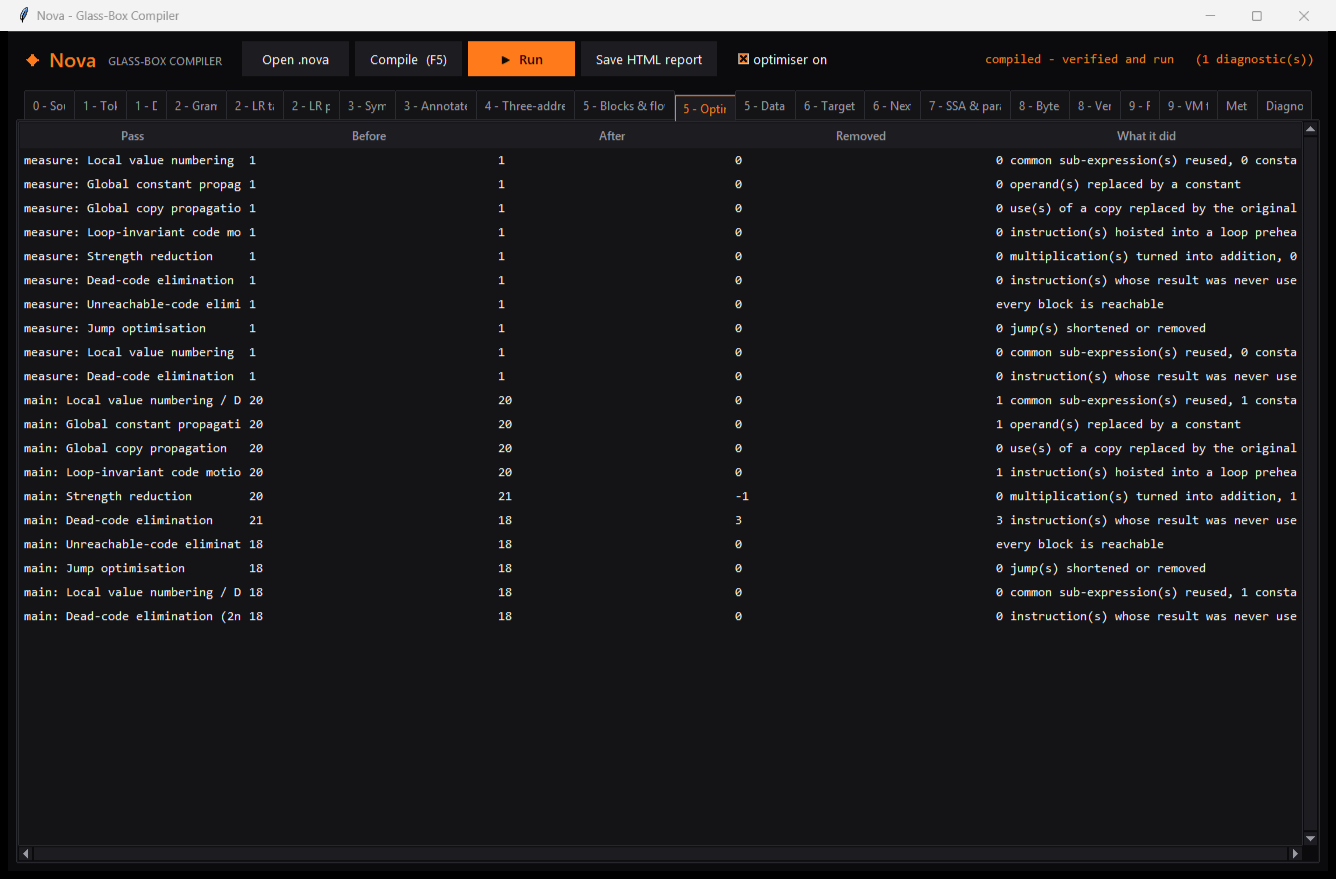
\includegraphics[width=0.49\textwidth]{figures/desktop-viewer.png}\label{fig:desktop-a}}
\hfil
\subfloat[Run tab: output, step counts and the activation-record stack of the Fibonacci program]{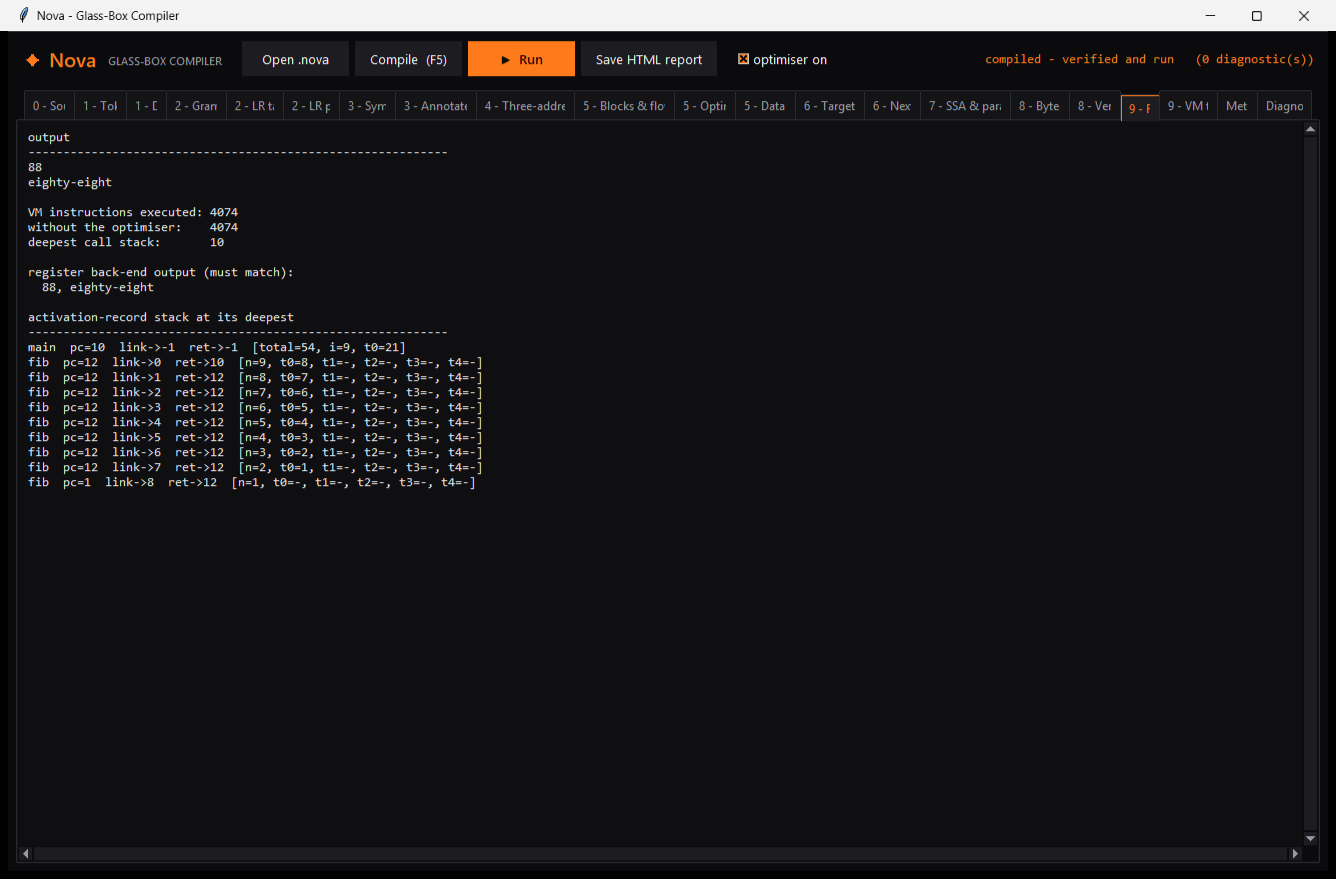
\includegraphics[width=0.49\textwidth]{figures/desktop-run.png}\label{fig:desktop-b}}\\[4pt]
\subfloat[Verifier tab: the six properties proved for each of the three functions of \code{03\_gcd.nova}]{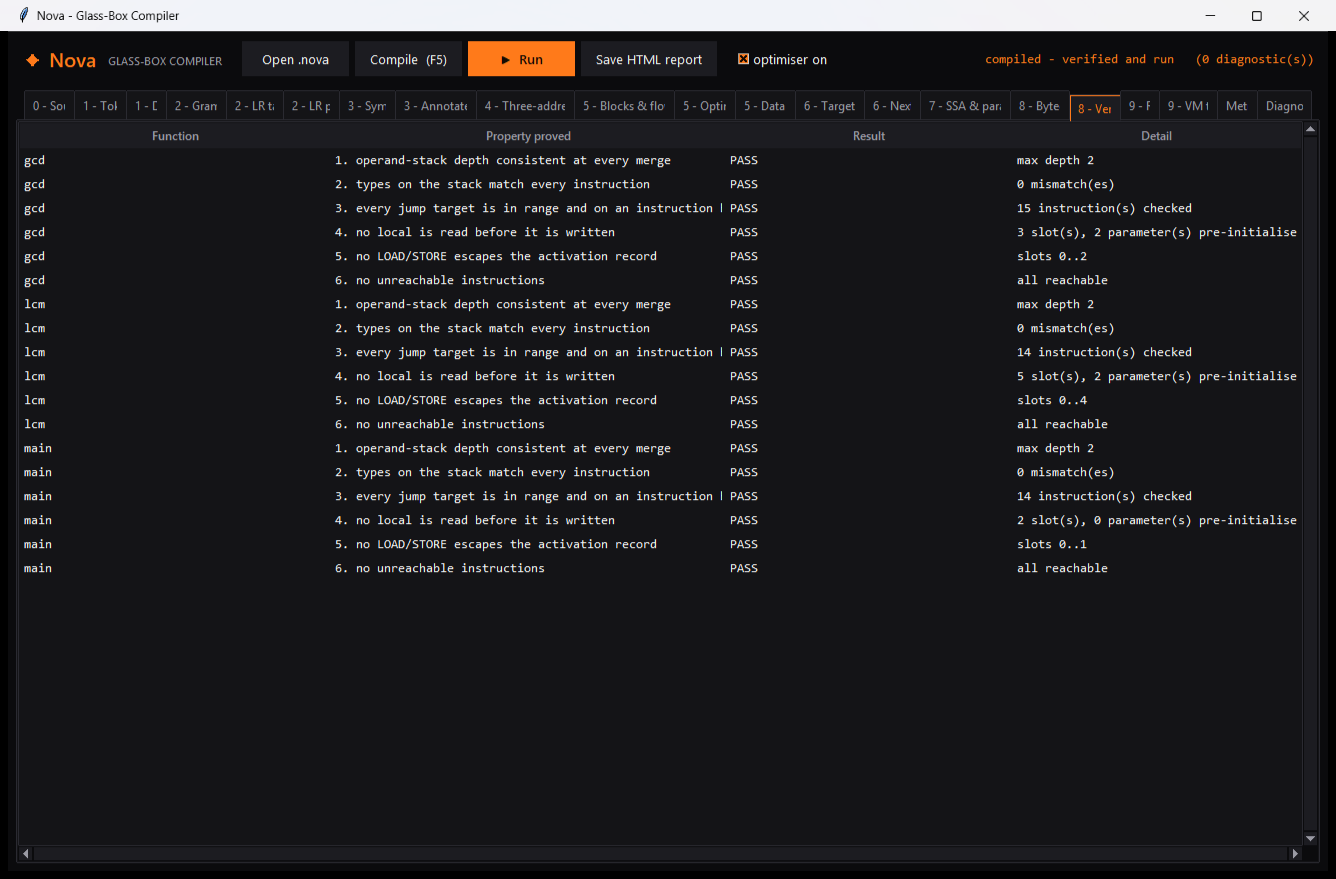
\includegraphics[width=0.49\textwidth]{figures/desktop-verifier.png}\label{fig:desktop-c}}
\caption{The desktop viewer (Tkinter), with one tab per phase, in the same black-and-orange visual identity as the studio. It needs no browser and no server, only the Python installer's own Tkinter.}
\label{fig:desktop}
\end{figure*}

\begin{figure*}[!t]
\centering
\subfloat[Tokens tab: kind, lexeme, position and attribute]{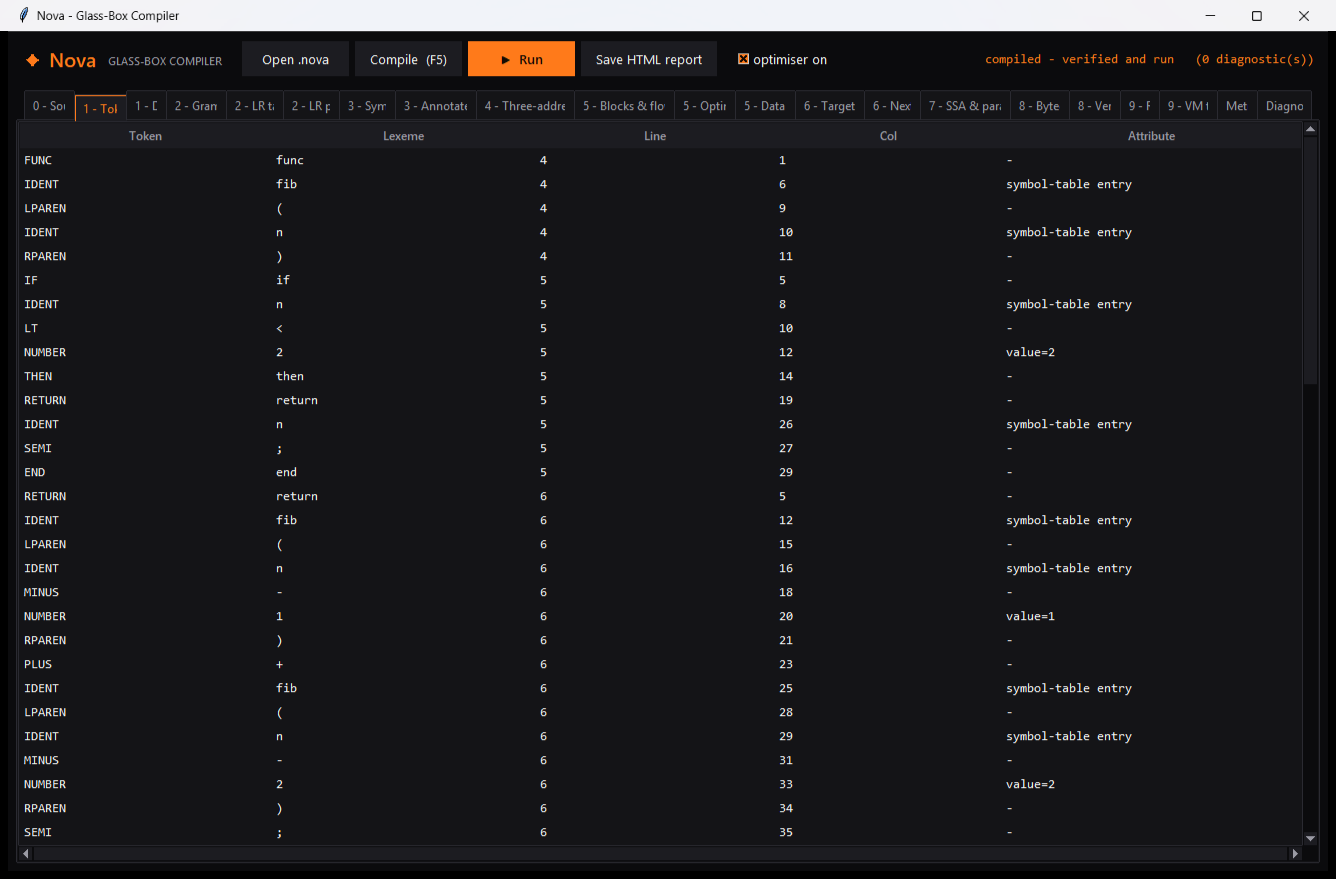
\includegraphics[width=0.49\textwidth]{figures/desktop-tokens.png}\label{fig:desktop2-a}}
\hfil
\subfloat[LR parse tab: the 297 steps of the LALR(1) parse]{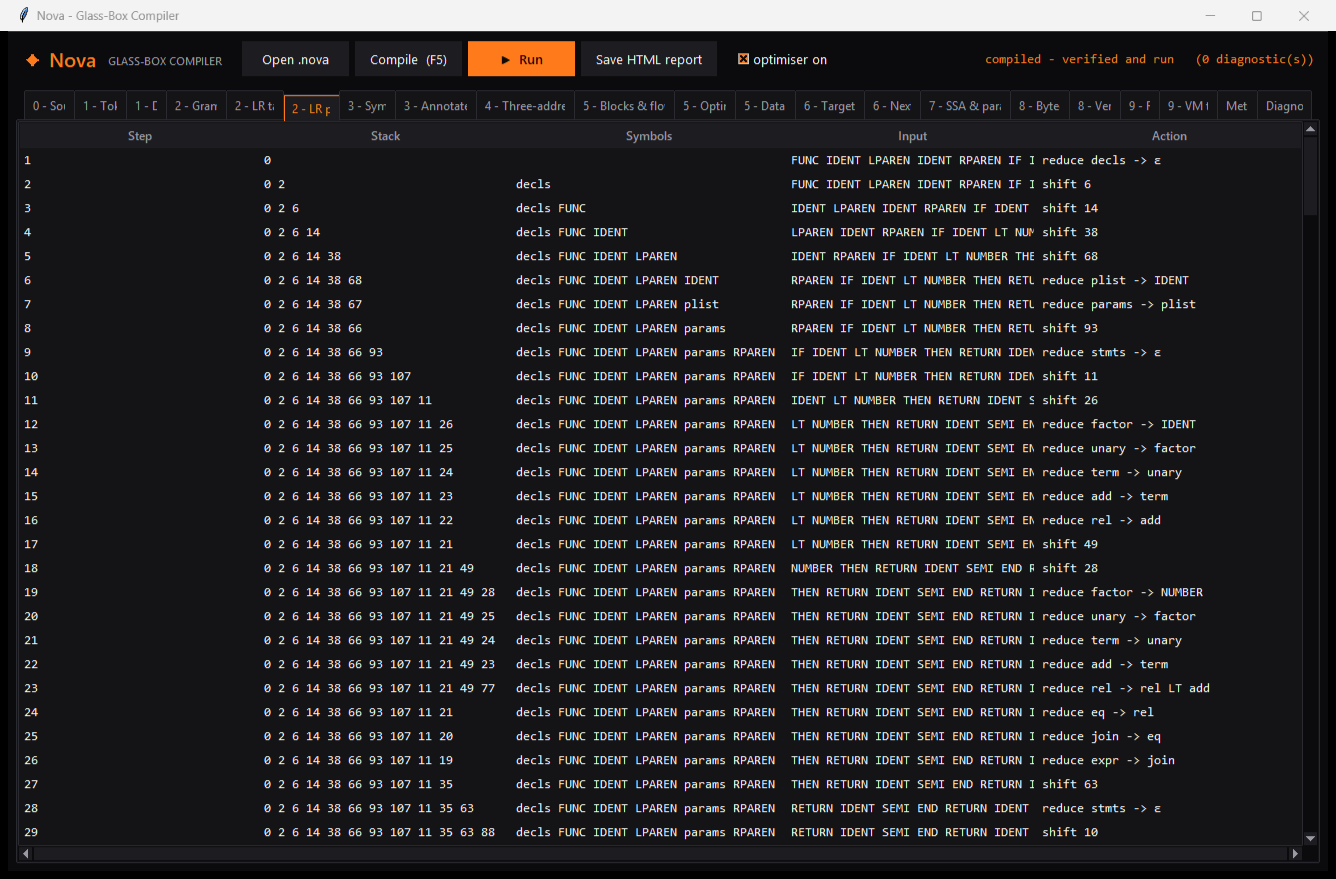
\includegraphics[width=0.49\textwidth]{figures/desktop-parse.png}\label{fig:desktop2-b}}\\[4pt]
\subfloat[Data-flow tab: the four analyses of \code{03\_gcd.nova}]{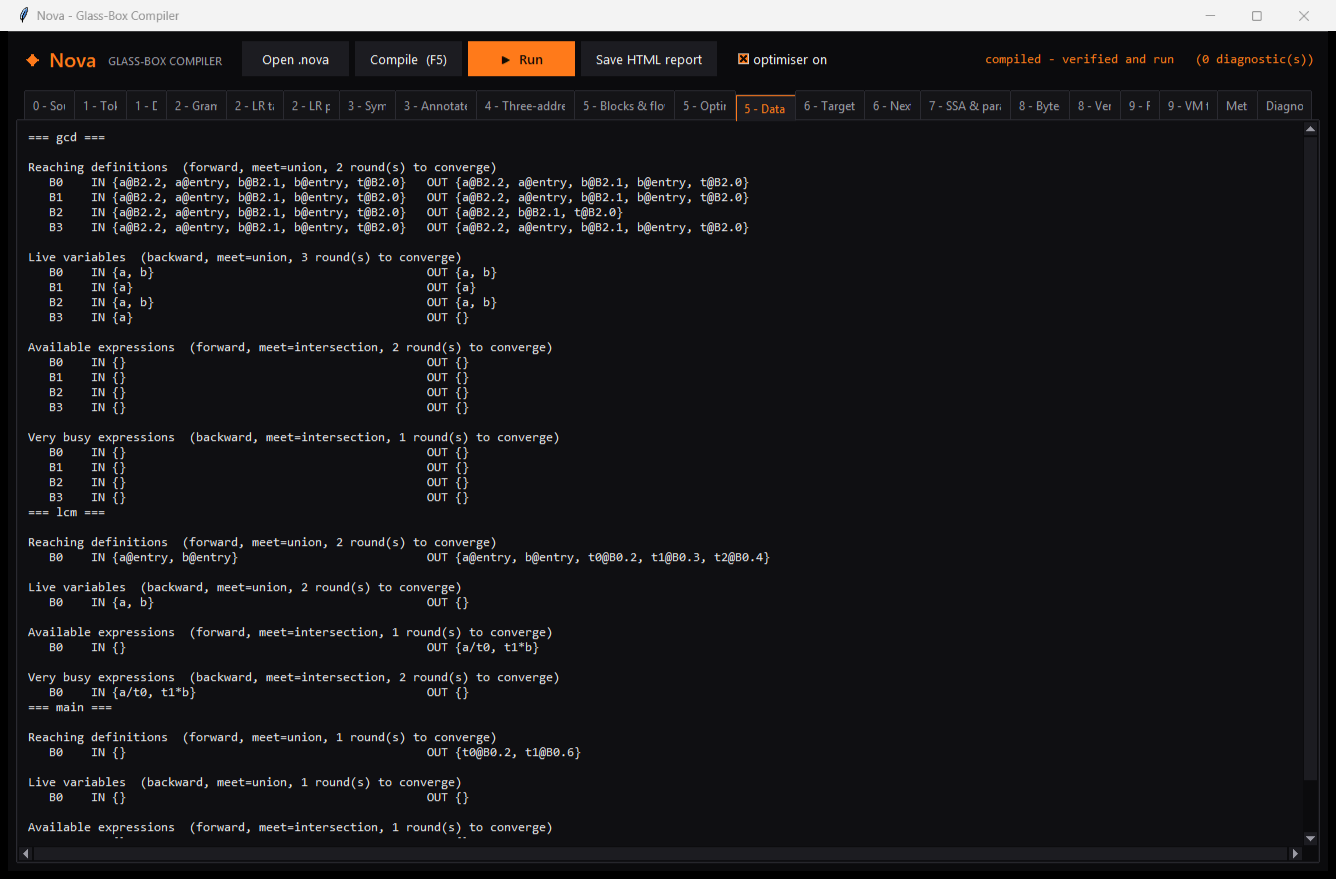
\includegraphics[width=0.49\textwidth]{figures/desktop-dataflow.png}\label{fig:desktop2-c}}
\hfil
\subfloat[SSA tab: \code{06\_parallel.nova} with its $\phi$-functions]{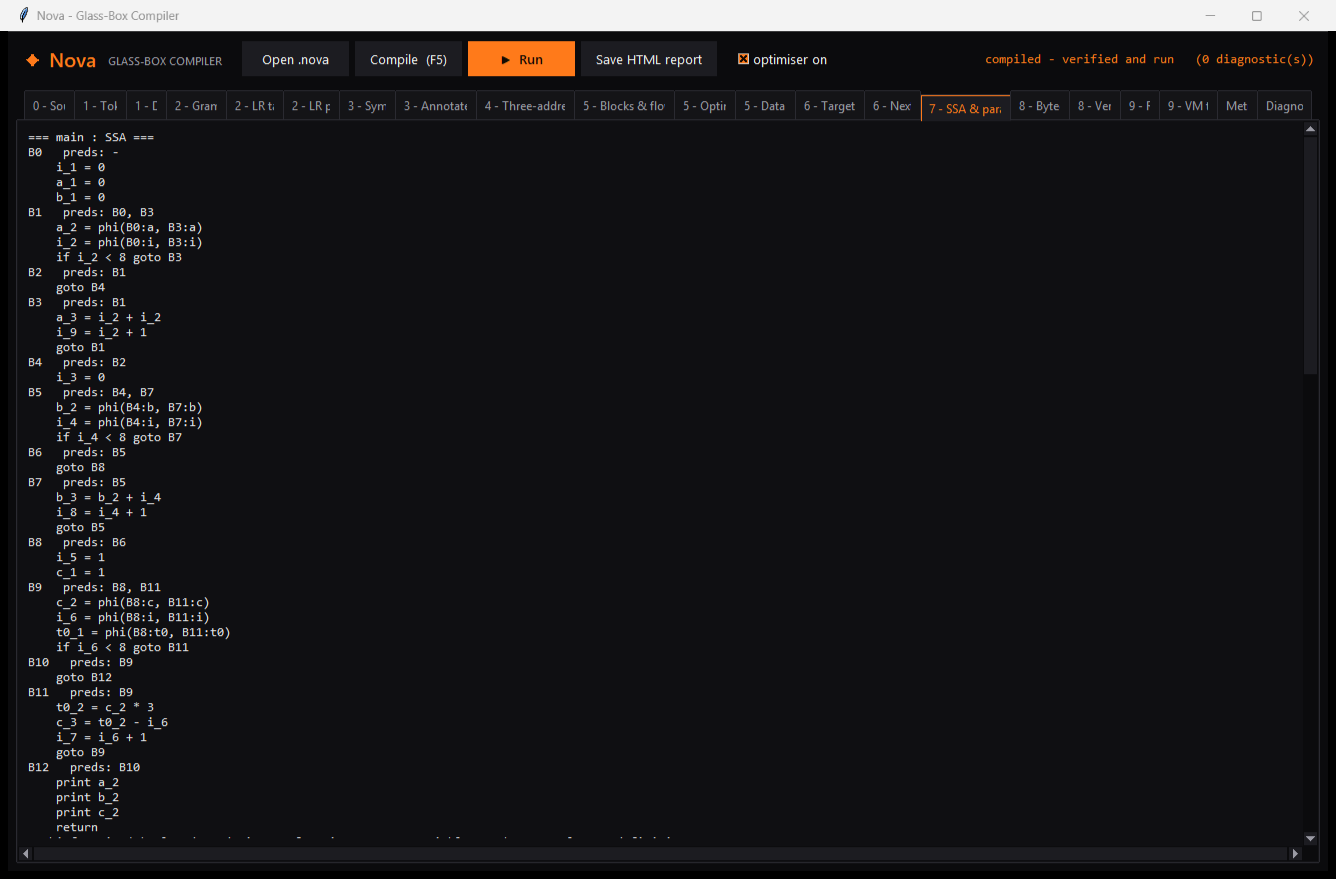
\includegraphics[width=0.49\textwidth]{figures/desktop-ssa.png}\label{fig:desktop2-d}}
\caption{Four more tabs of the desktop viewer. Every phase that the studio draws is available here as a table or a listing.}
\label{fig:desktop2}
\end{figure*}

\begin{figure*}[!t]
\centering
\subfloat[Overview: the headline numbers and the source program]{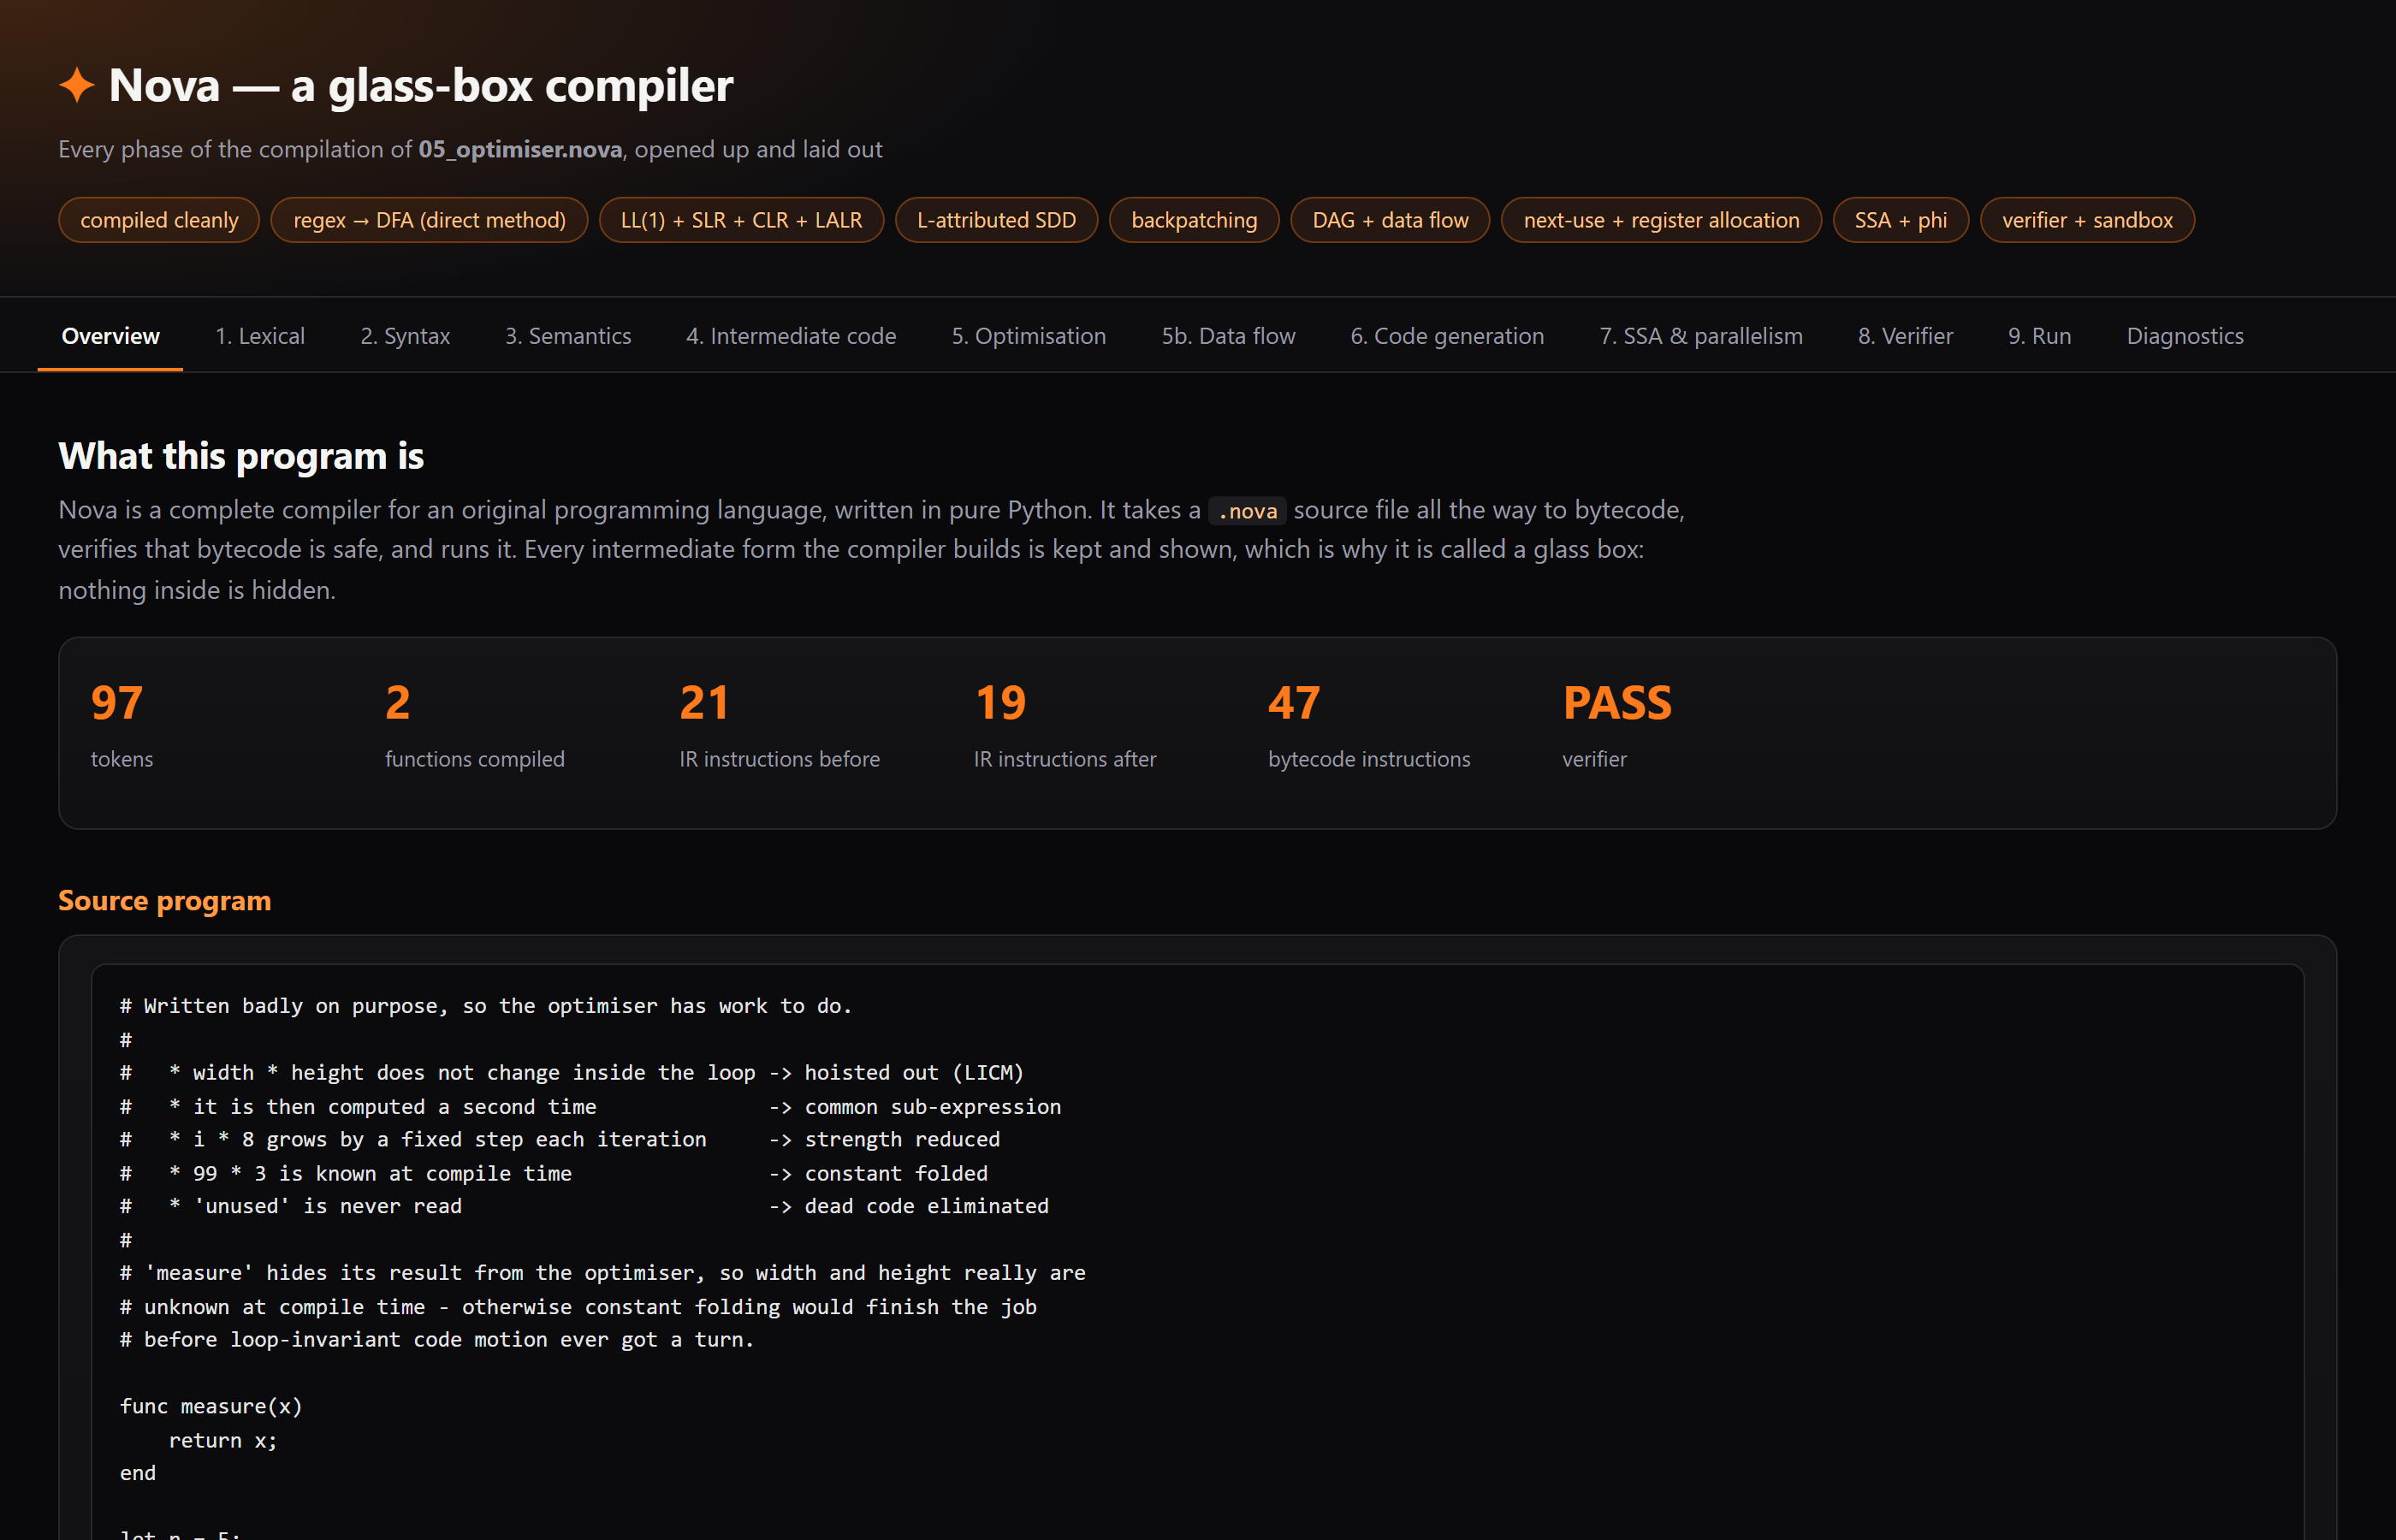
\includegraphics[width=0.49\textwidth]{figures/report-html-overview.png}\label{fig:report-a}}
\hfil
\subfloat[Optimisation: the flow graph of \code{main} before optimisation]{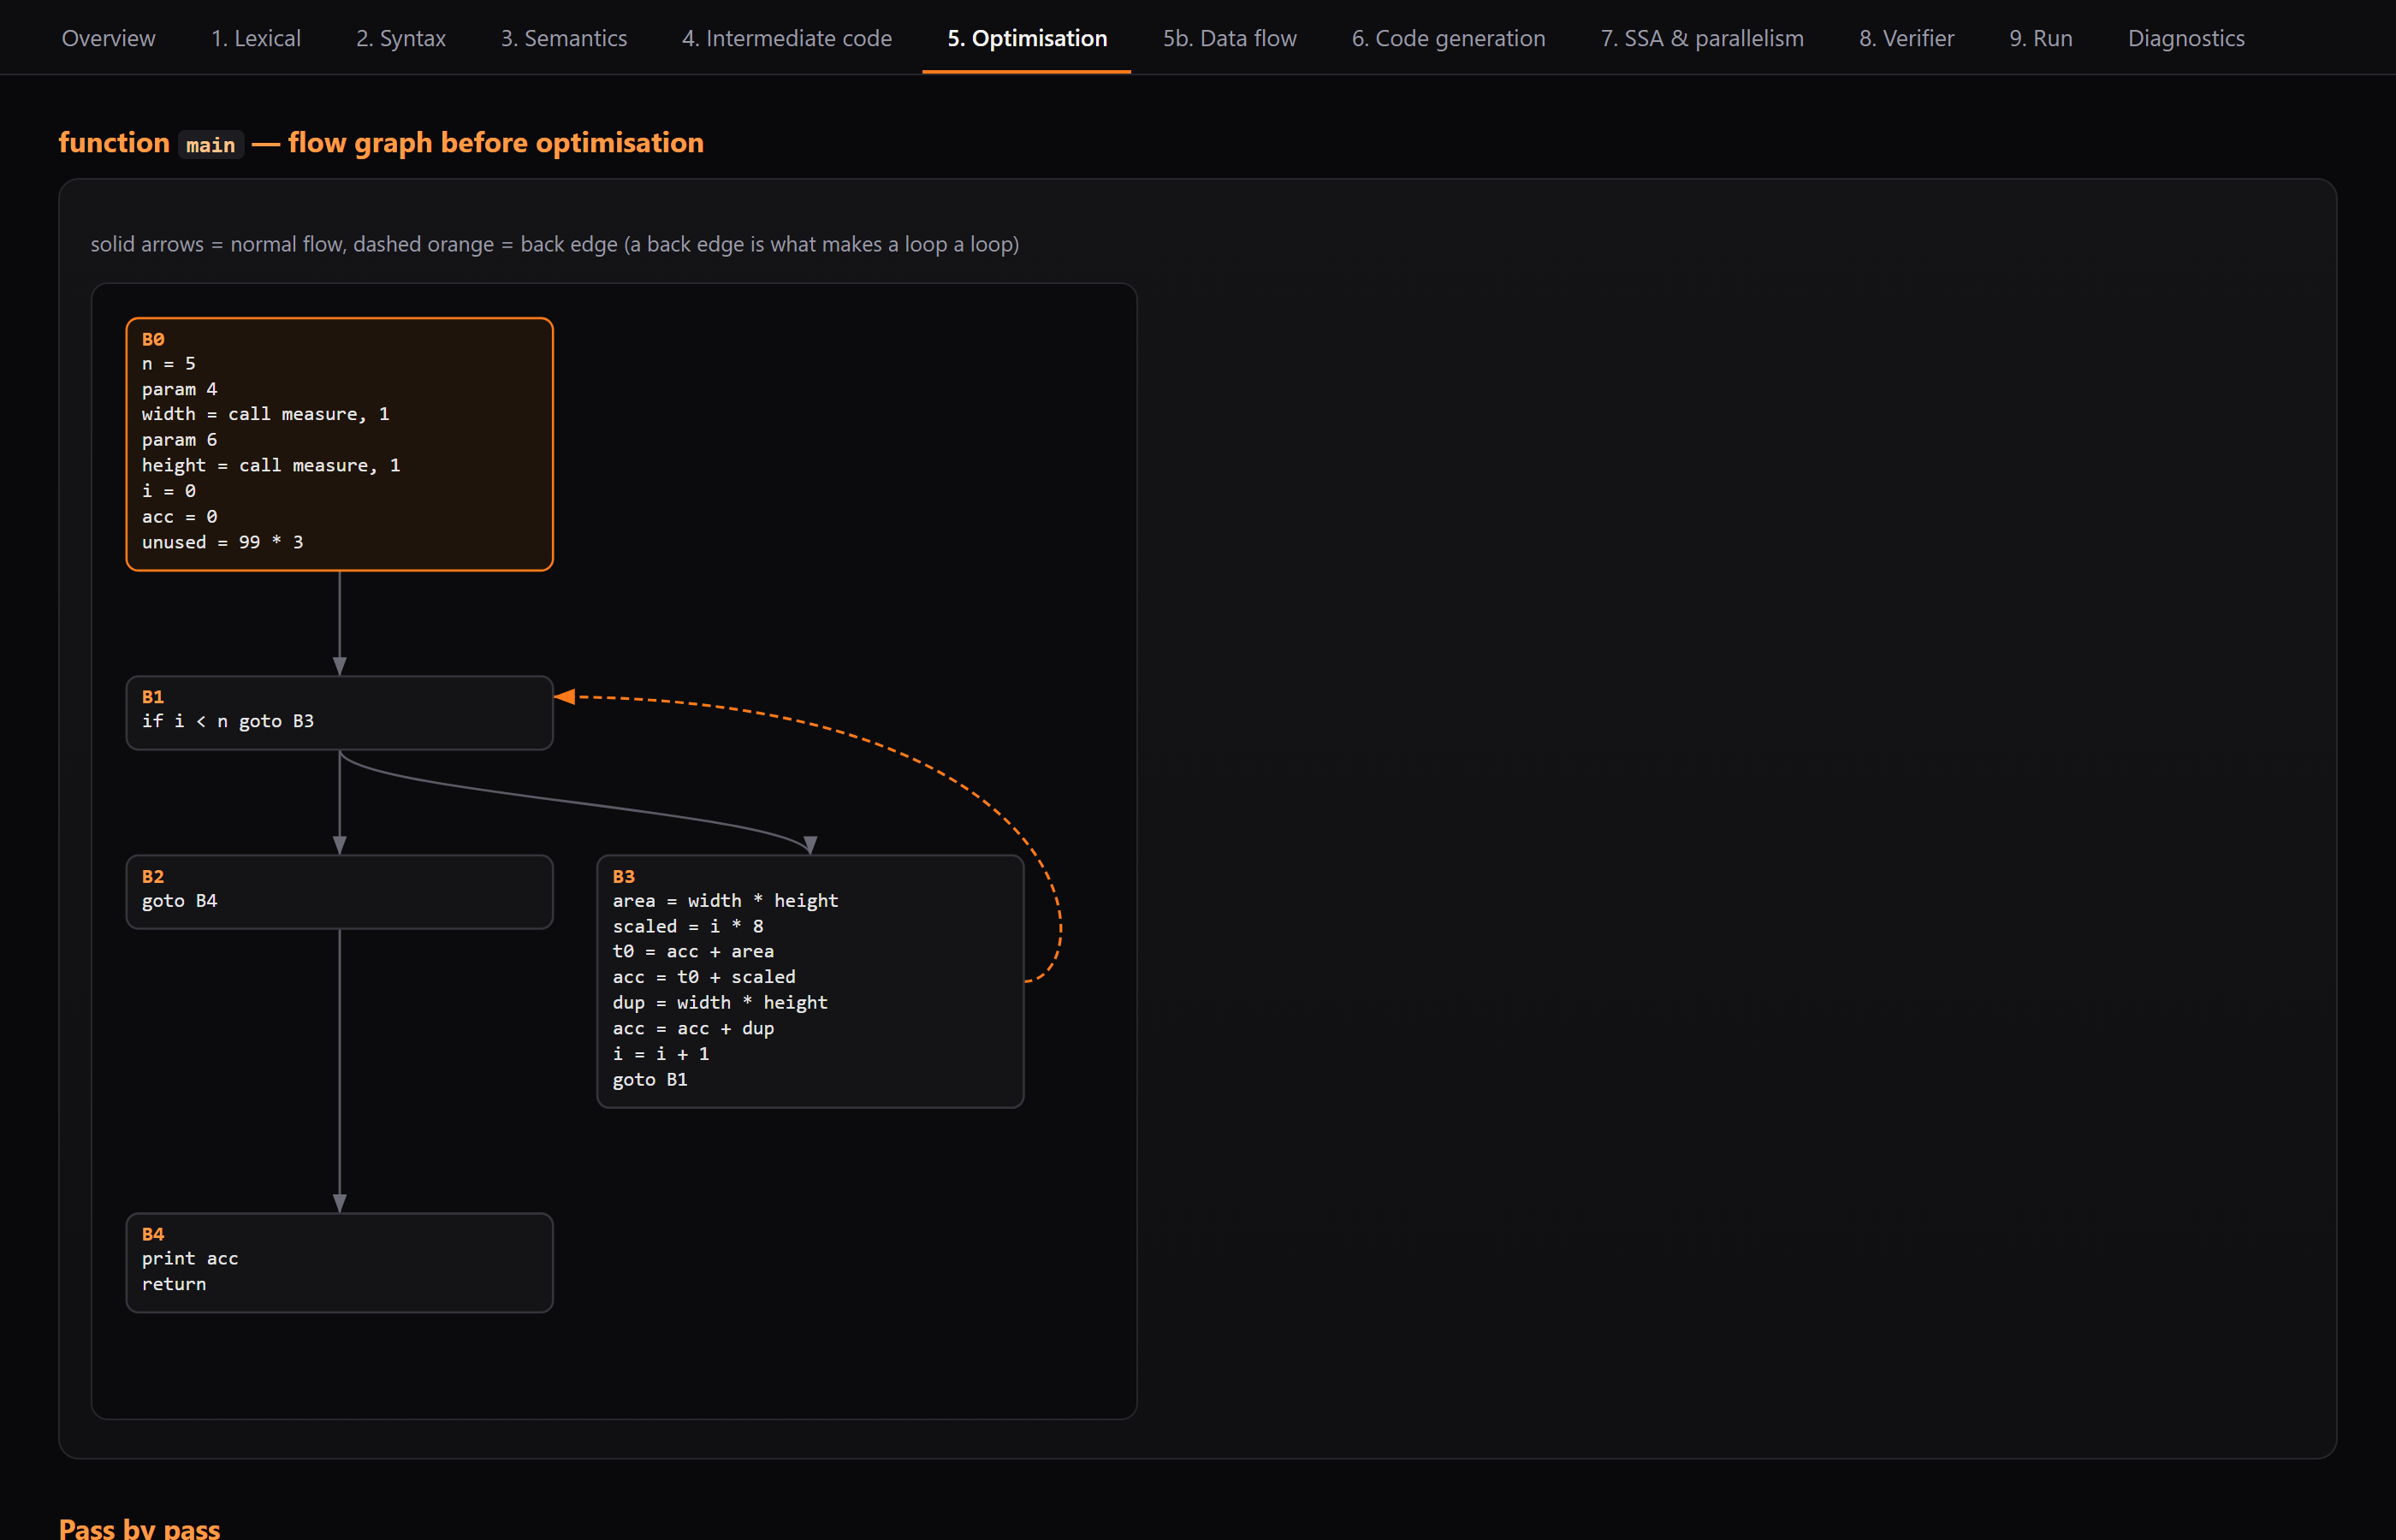
\includegraphics[width=0.49\textwidth]{figures/report-html.png}\label{fig:report-b}}\\[4pt]
\subfloat[SSA and parallelism: dominators and the SSA form of each function]{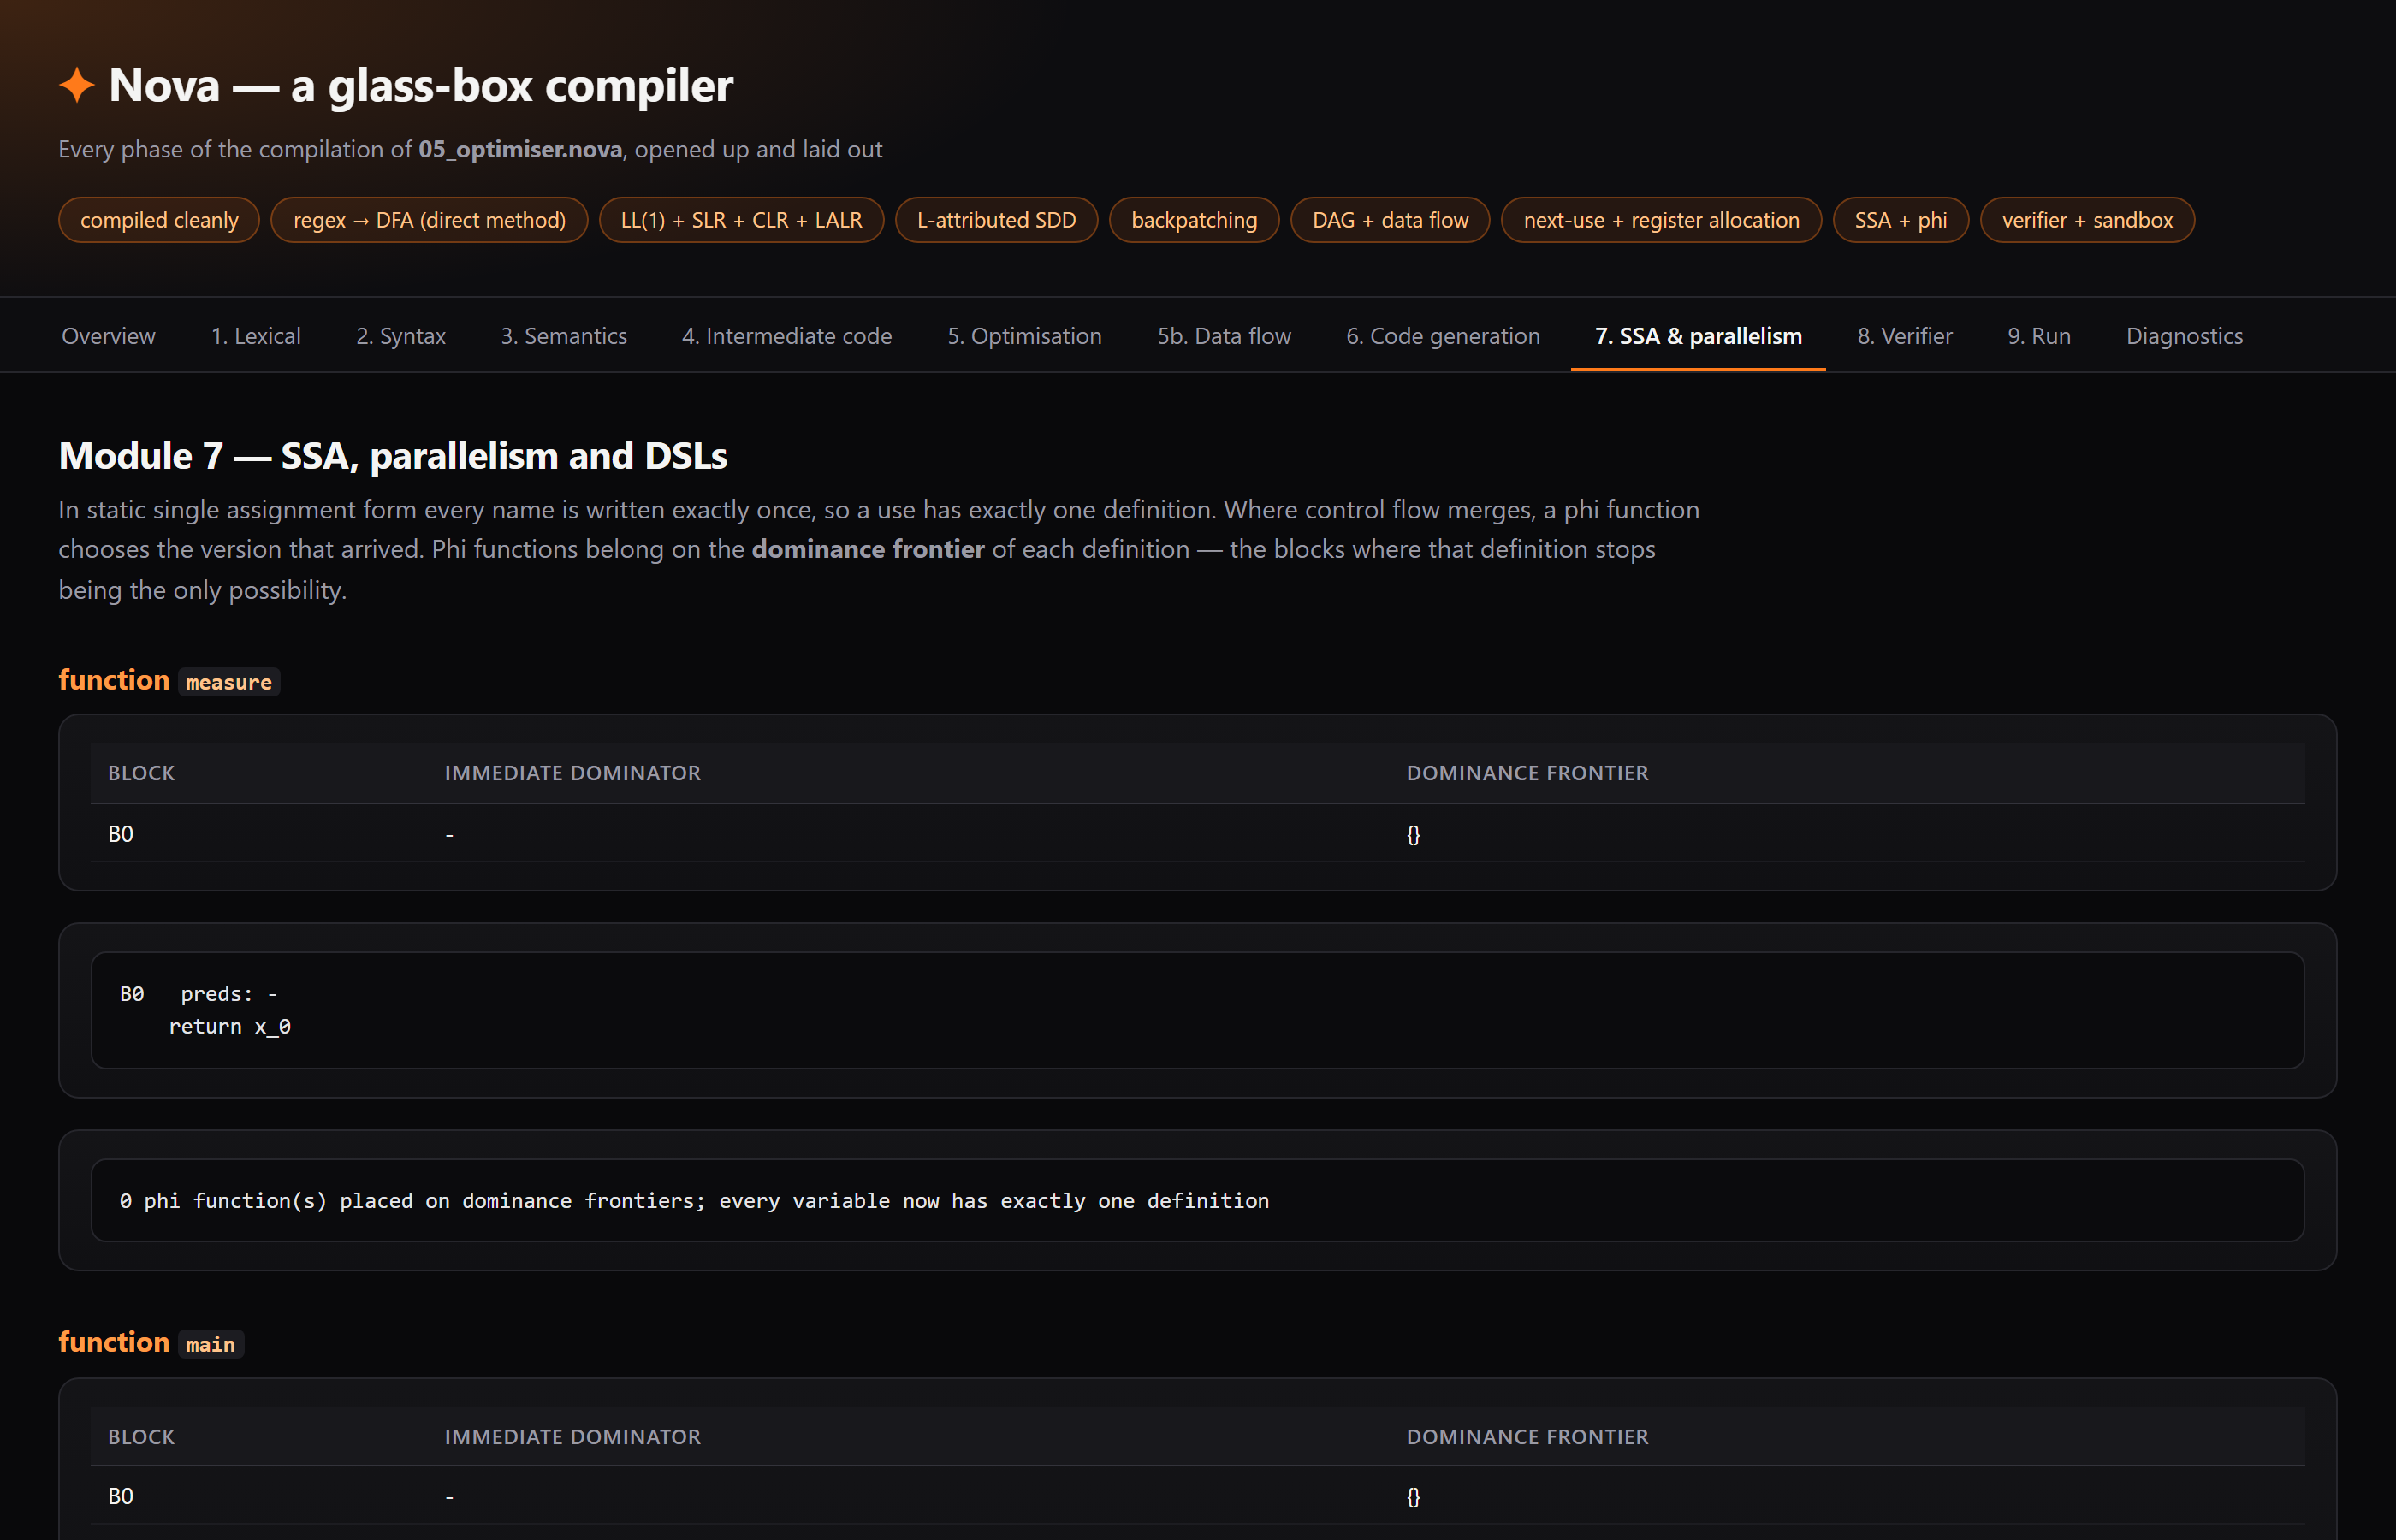
\includegraphics[width=0.49\textwidth]{figures/report-html-ssa.png}\label{fig:report-c}}
\caption{The self-contained HTML report for \code{05\_optimiser.nova}, which embeds every phase and its flow graphs in one file with no external resources.}
\label{fig:report}
\end{figure*}

\begin{figure*}[!t]
\centering
\subfloat[Lexical section: the DFA statistics and the token specifications]{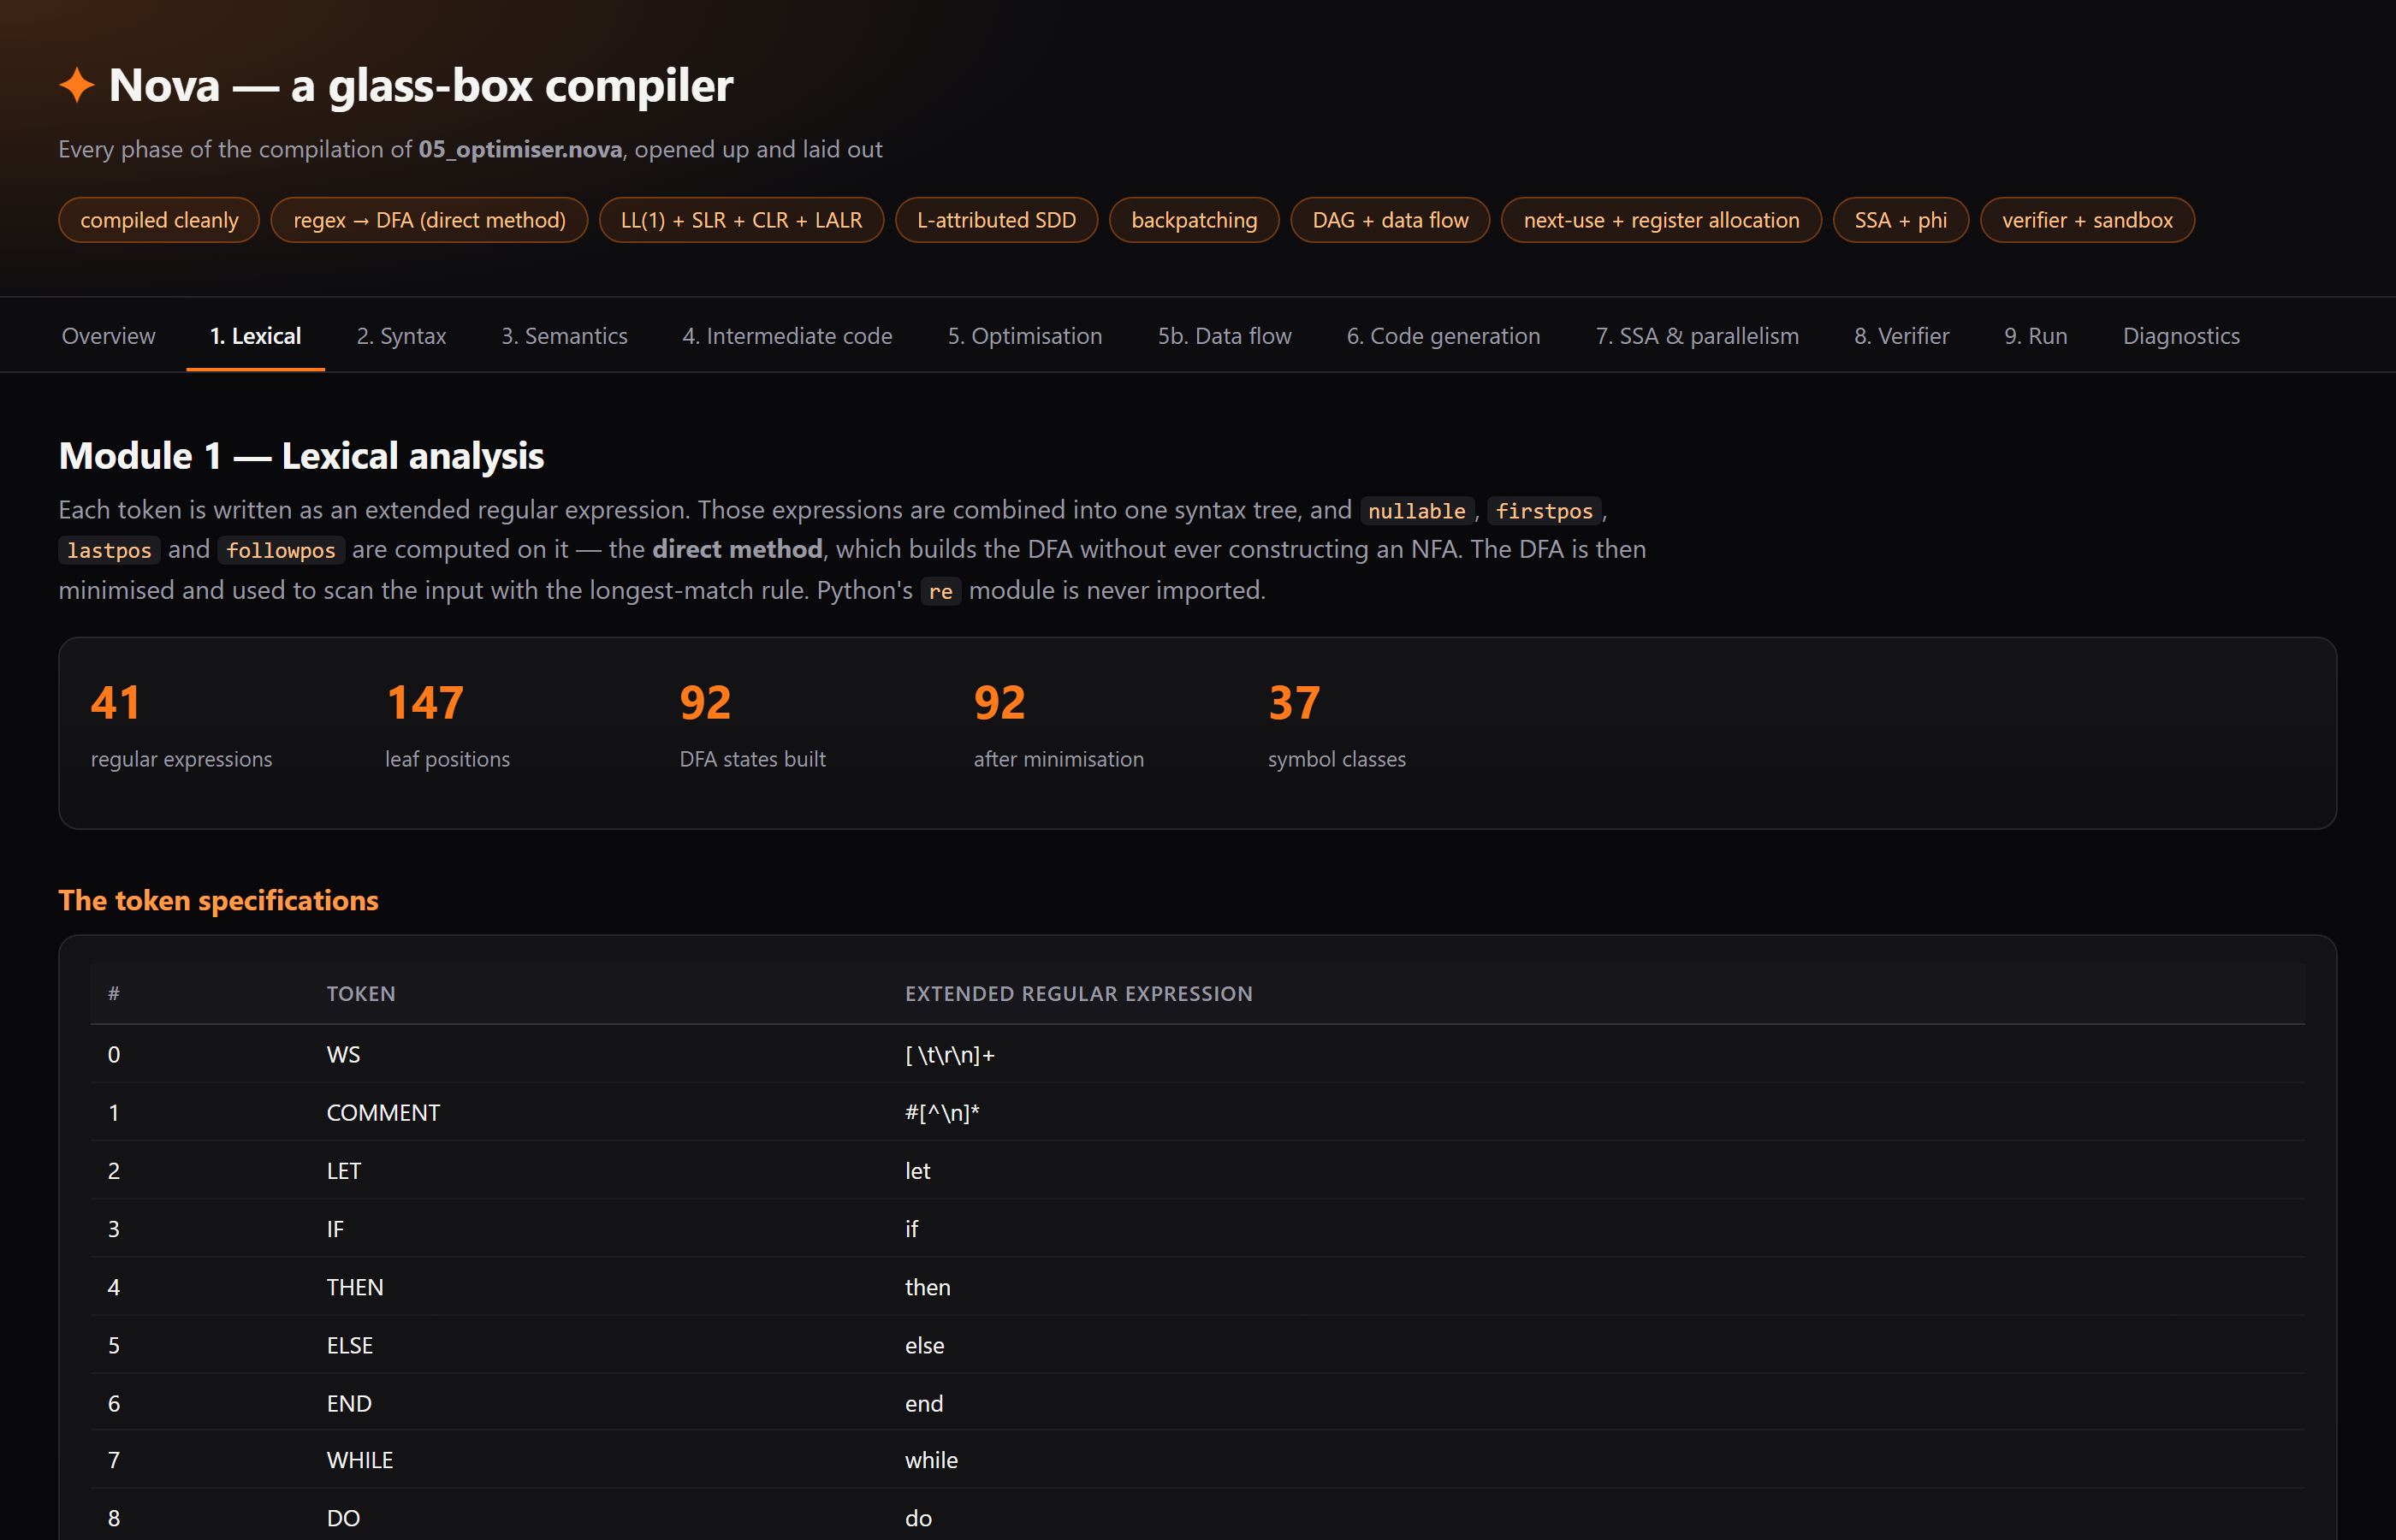
\includegraphics[width=0.49\textwidth]{figures/report-html-lexical.png}\label{fig:report2-a}}
\hfil
\subfloat[Code-generation section: activation record and next-use information]{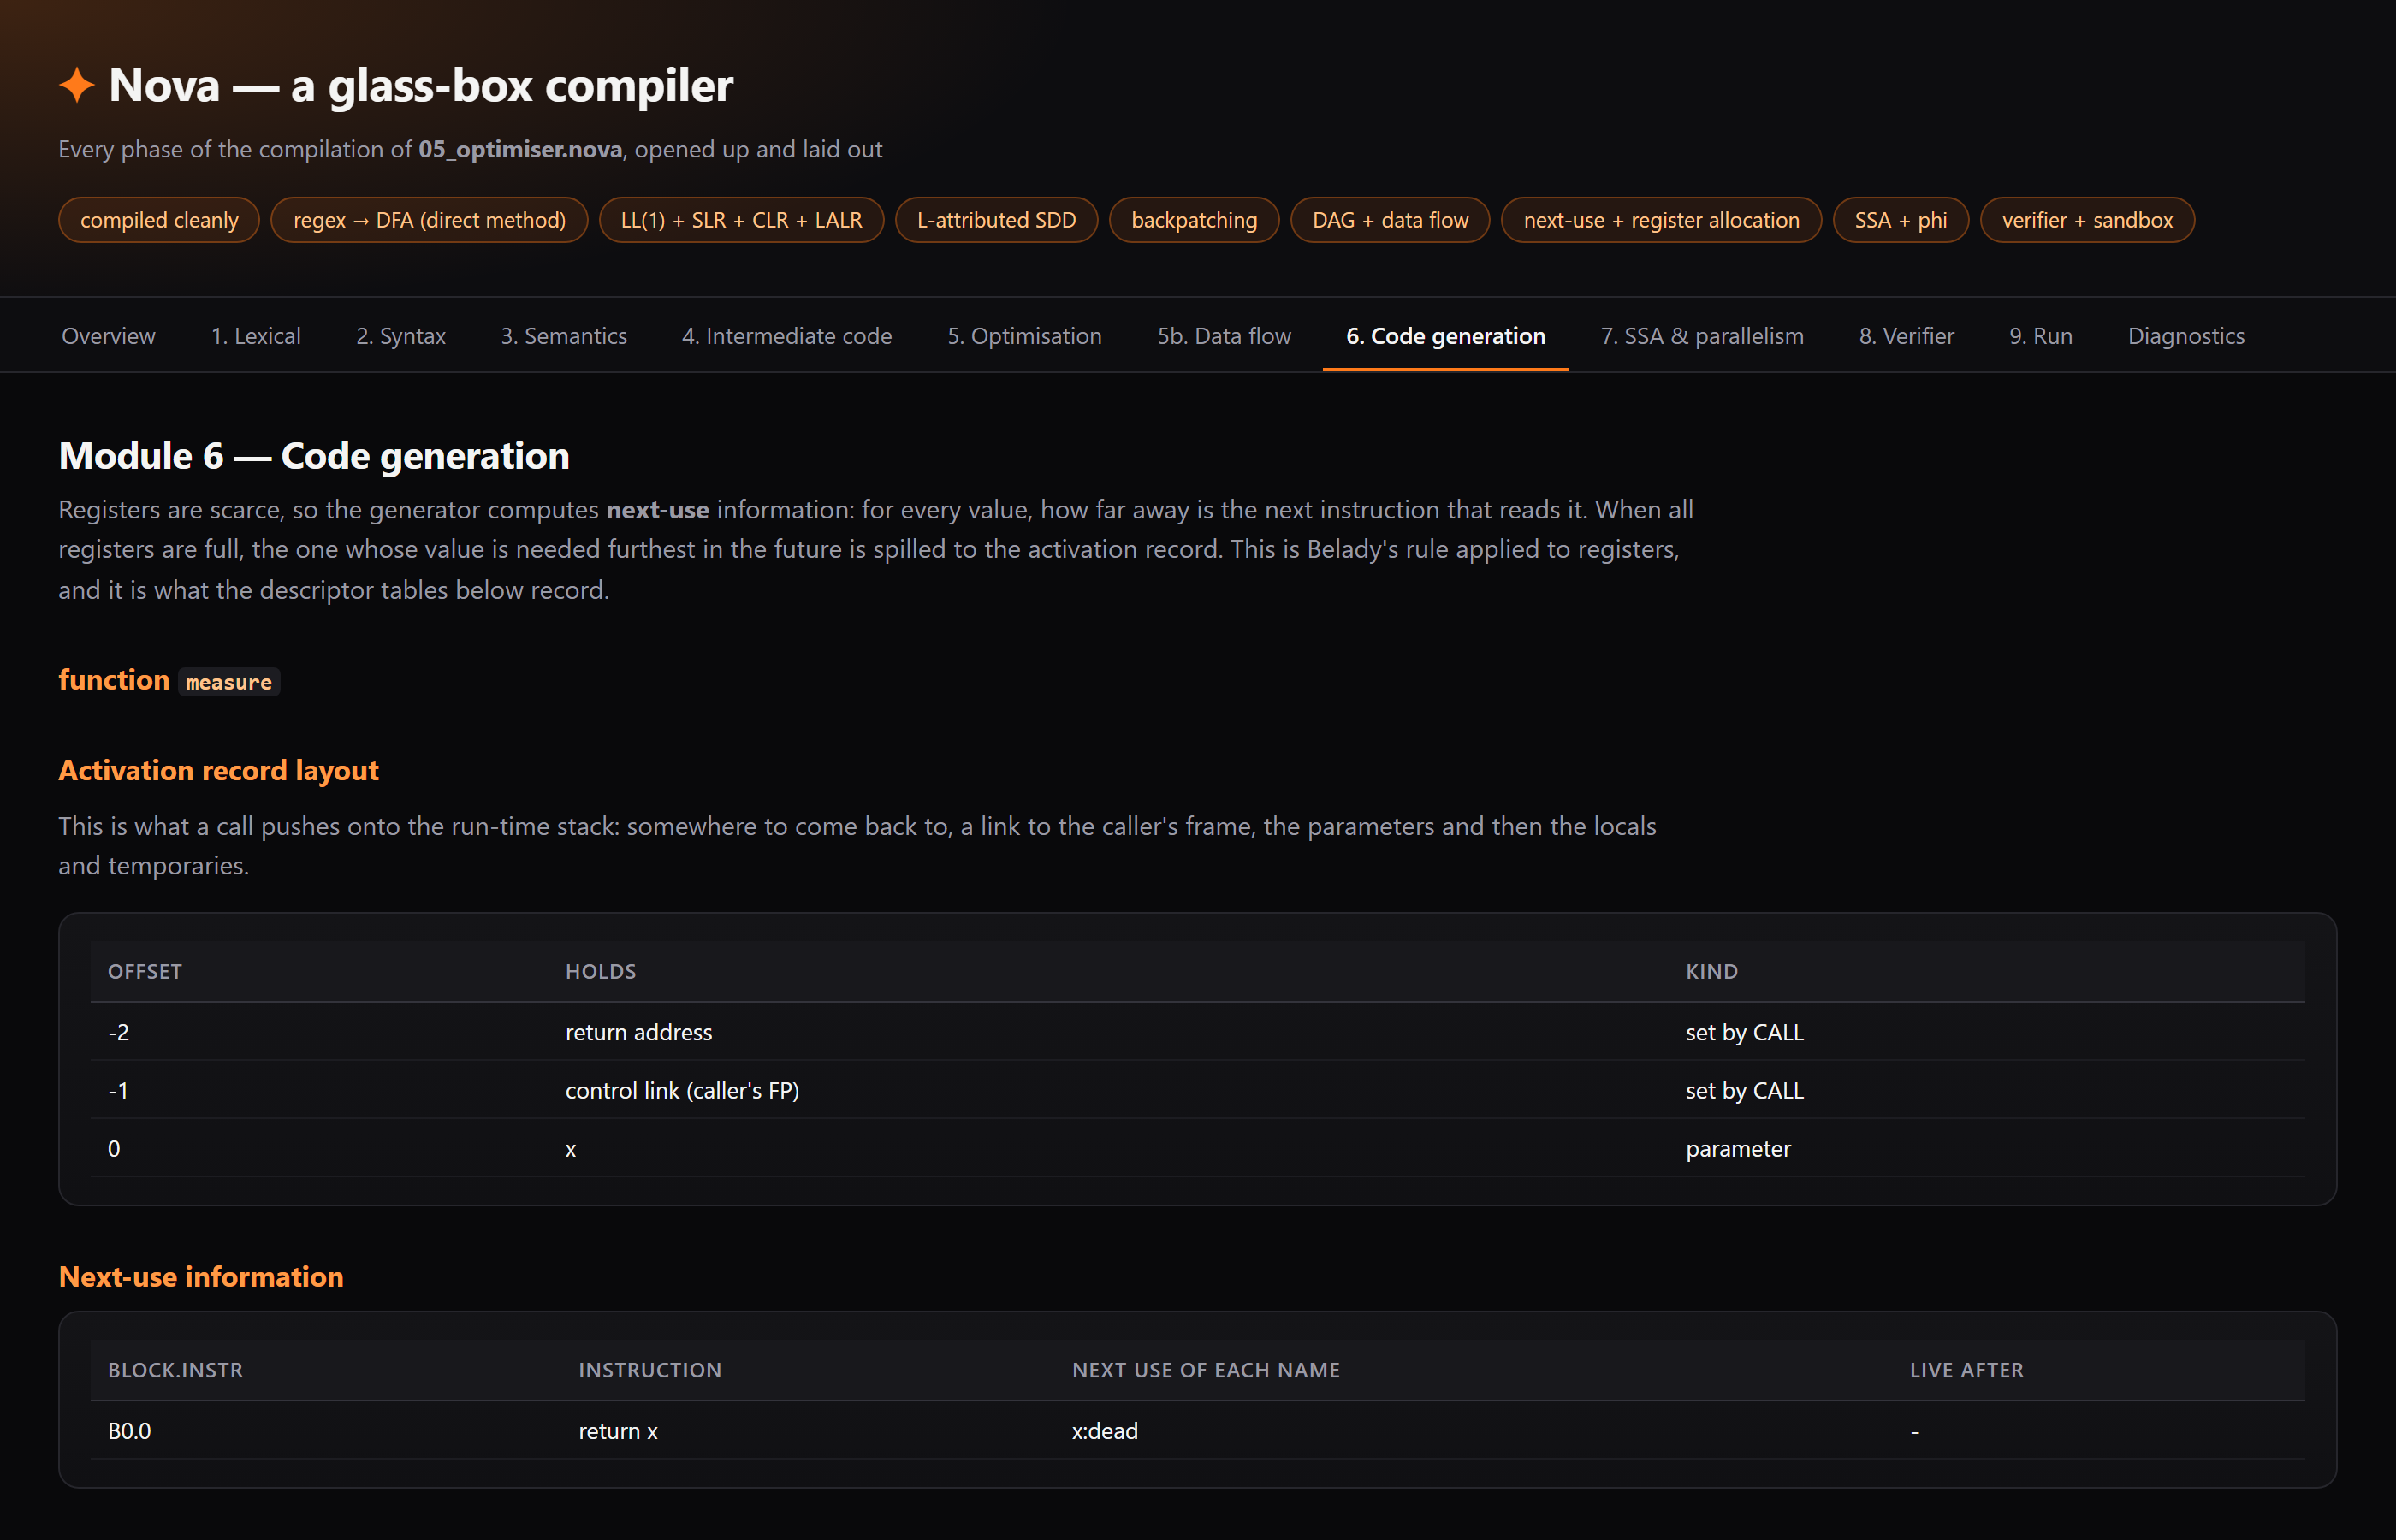
\includegraphics[width=0.49\textwidth]{figures/report-html-codegen.png}\label{fig:report2-b}}\\[4pt]
\subfloat[Run section: step counts, output and the activation-record stack]{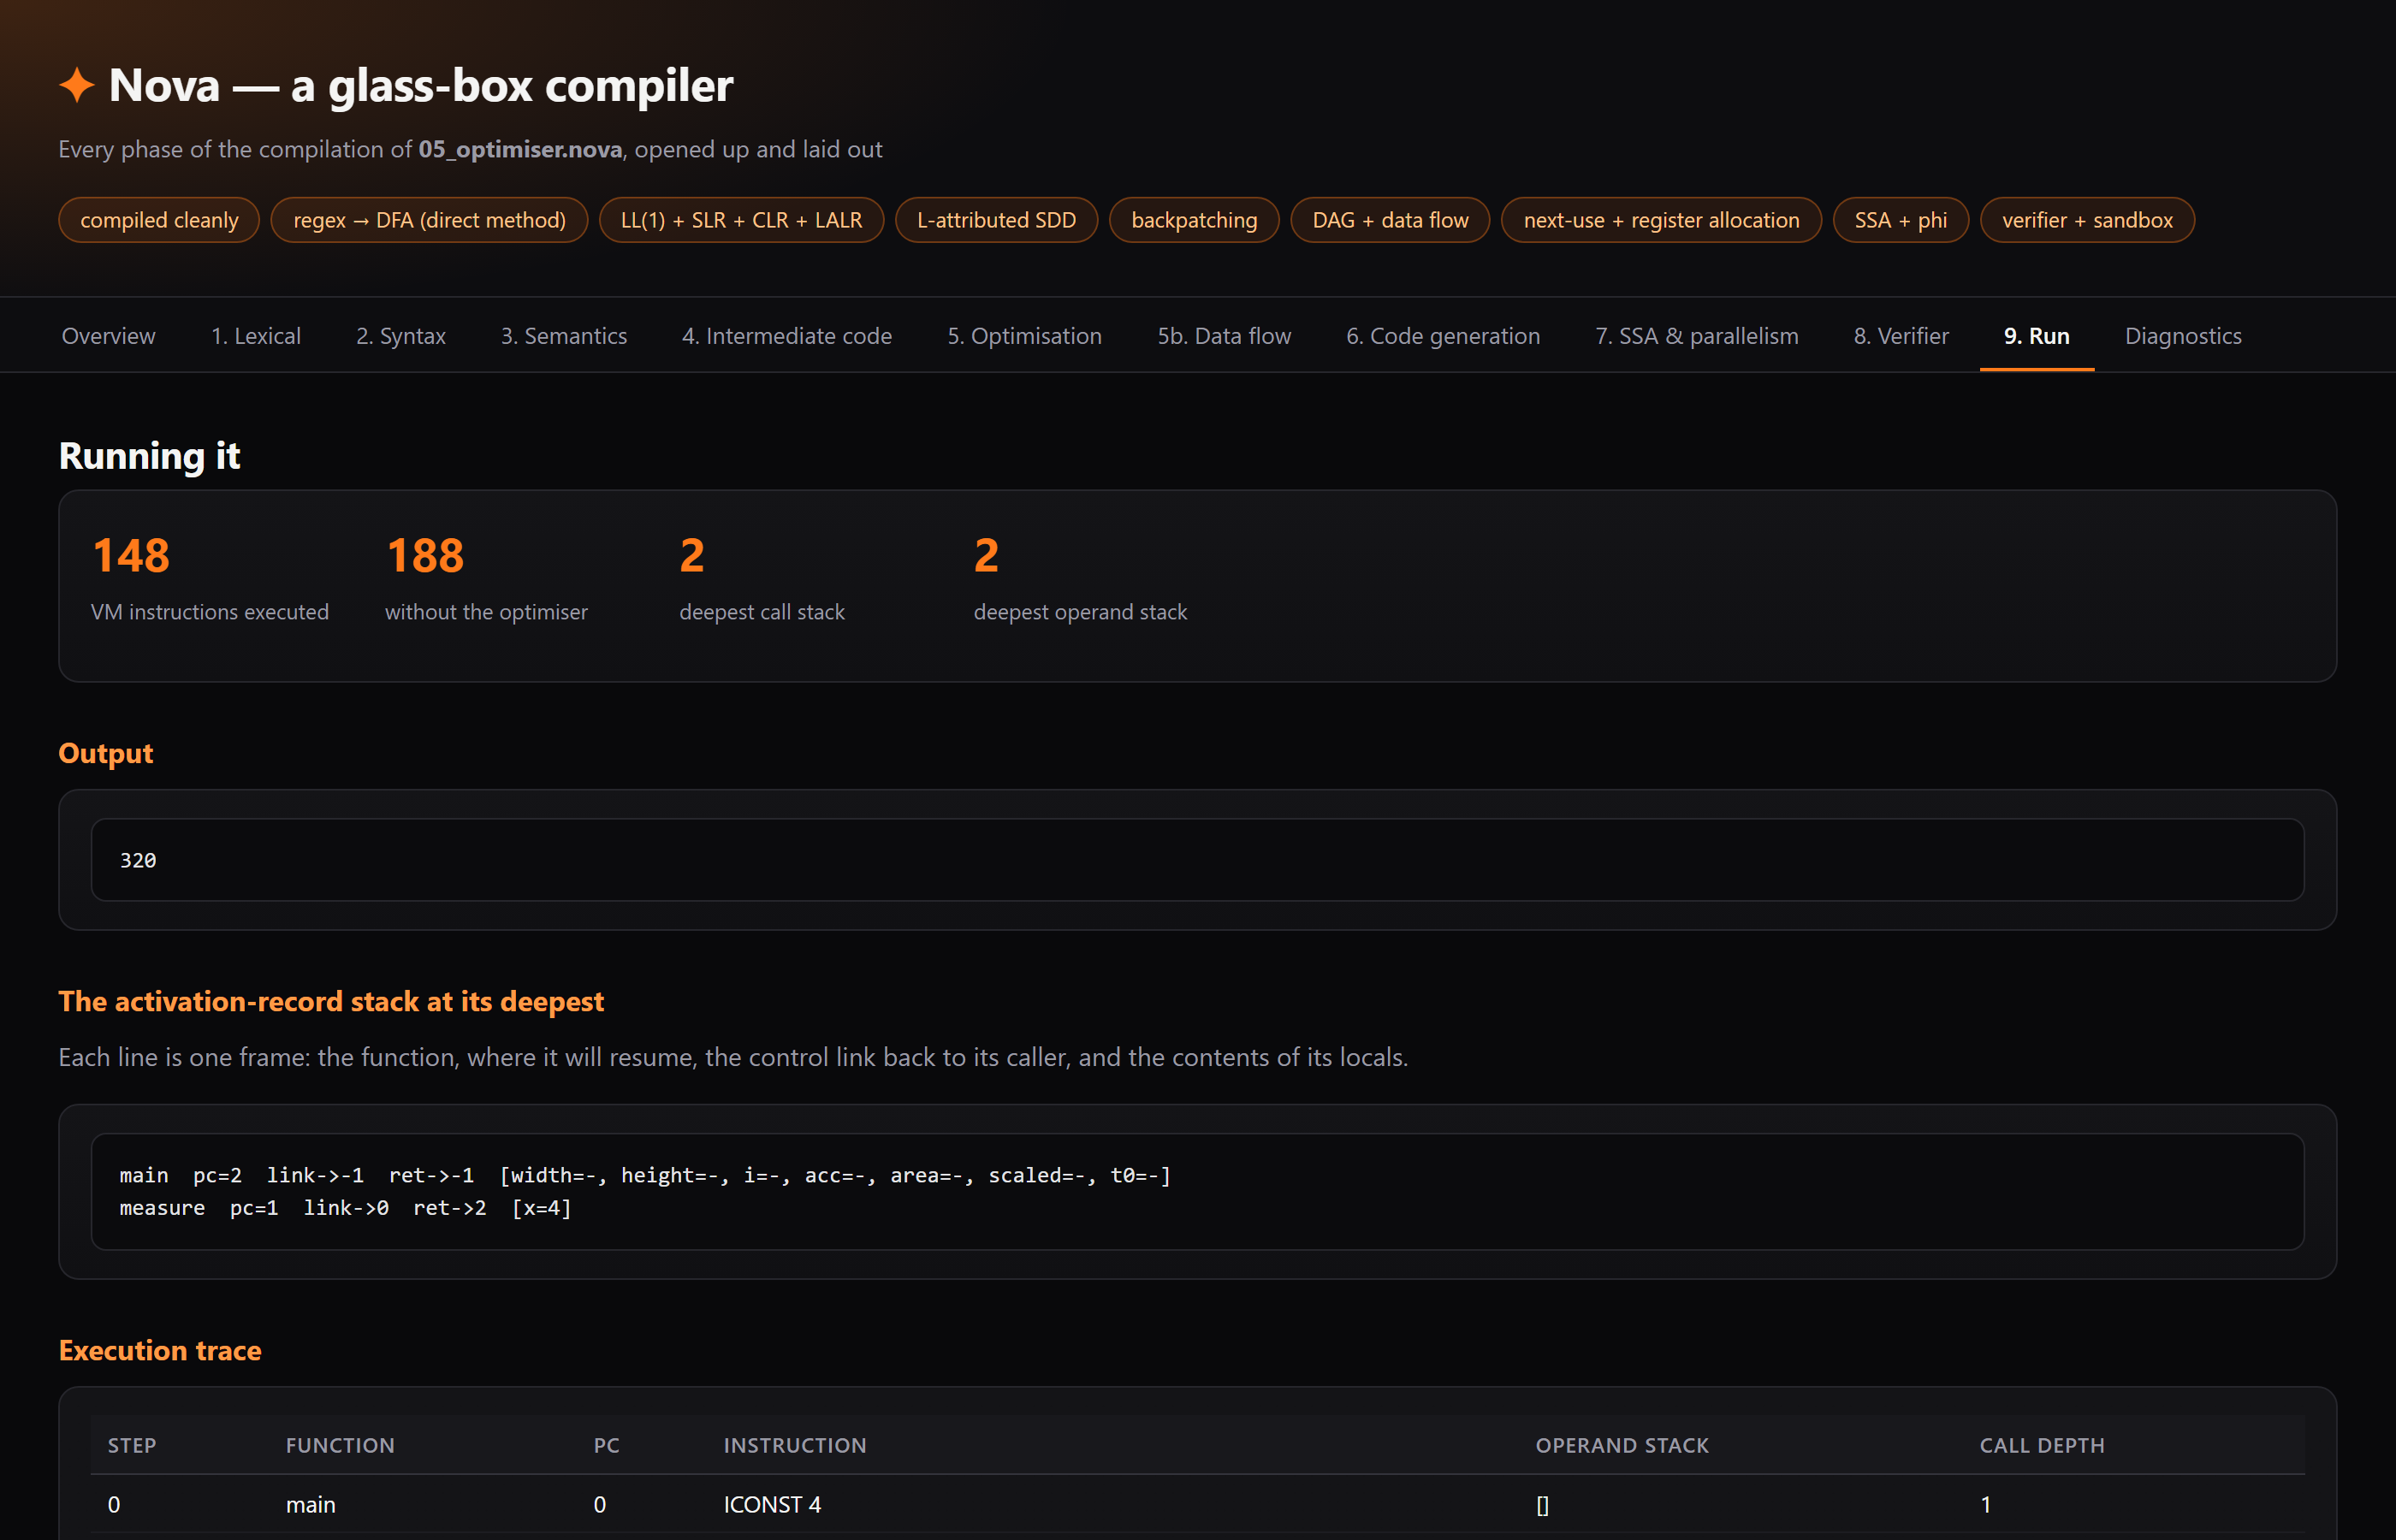
\includegraphics[width=0.49\textwidth]{figures/report-html-run.png}\label{fig:report2-c}}
\caption{Three more sections of the HTML report for \code{05\_optimiser.nova}.}
\label{fig:report2}
\end{figure*}

\subsection{Limitations and Threats to Validity}
Nova deliberately trades breadth for transparency, which imposes seven limitations:
\begin{itemize}
\item The language has no arrays, records or heap, so the dependence analysis reasons about scalars only and cannot compute dependence distances.
\item Register allocation is local to basic blocks.
\item LALR(1) is built from the canonical collection rather than by look-ahead propagation.
\item The abstract domain of the verifier is coarse (\code{int}, \code{str}, \code{any}).
\item Execution is interpreted in Python, and the deepest-stack snapshot costs $O(d^2)$ frame renderings for a recursion of depth $d$.
\item The bookkeeping of modules 5--7 grows between quadratically and cubically with program size, which limits instantaneous feedback to programs of roughly a hundred lines.
\item Nova Studio is a single-user local tool.
\end{itemize}
Three threats bear on the evaluation itself:
\begin{itemize}
\item \emph{External validity.} The benchmark suite is small and was written alongside the compiler, so the optimisation figures describe these programs rather than real-world code, and the scaling series is made of copies of one loop.
\item \emph{Internal validity.} Timings come from one machine on battery power under normal desktop load; we mitigated noise with medians, CPU-time cross-checks, a separate server process and a recorded power state, and the relative comparisons were stable across repeated sessions, including a mains-powered one that ran about $3.5\times$ faster.
\item \emph{Construct validity.} The educational benefit is argued from coverage, engagement design and the visualisation literature, not yet measured with learners.
\end{itemize}

% =============================================================================
\clearpage
\section{Conclusions and Future Work}
\label{sec:conclusion}
This paper presented Nova, a glass-box compiler that takes an original language from regular expressions to verified, sandboxed execution while retaining and displaying every artefact on the way, and Nova Studio, which turns those artefacts into instruments a learner can operate. The evaluation shows six results:
\begin{itemize}
\item The classical claims of compiler theory hold when measured. LALR(1) keeps SLR(1)'s 116 states with 75\% fewer entries than CLR(1), and every data-flow analysis converges within the $d+2$ passes that theory predicts, including the doubly nested loop that needs four.
\item Optimisation never changed a program's output, and the three independent back-ends agreed on every one of ten programs.
\item The verifier and the sandbox stopped all eight hostile programs, six statically and two at run time.
\item Compilation is fast enough for keystroke-level feedback on programs of the size used in a course---under 40\,ms for nine of ten benchmarks even on a throttled laptop---and a scaling study locates precisely where the glass box's bookkeeping grows superlinearly.
\item Making the internals visible exposed six latent defects that output-based testing had missed.
\item The approach needs nothing beyond a standard Python installation and a browser.
\end{itemize}

Future work follows directly from the limitations:
\begin{enumerate}
\item replacing the iterative dominator computation by the Cooper--Harvey--Kennedy algorithm~\cite{cooper2001}, solving the data-flow analyses with worklists over bit-vectors, and recording per-pass code as diffs, so that the middle end scales linearly in practice and the deepest-stack snapshot is taken once;
\item adding arrays and subscripted references, so that GCD and Banerjee dependence tests can compute distance vectors and drive loop distribution, fusion and interchange~\cite{kennedy1993,allen2001};
\item constructing LALR(1) by DeRemer--Pennello look-ahead propagation~\cite{deremer1982} and comparing it with the current core-merging method in the automaton browser;
\item global register allocation by graph colouring and by linear scan~\cite{chaitin1982,poletto1999}, visualised on the same timeline as the current local allocator;
\item SSA-based optimisation, such as sparse conditional constant propagation~\cite{wegman1991} and global value numbering, replacing the iterative passes;
\item a mechanised proof that the verifier is sound;
\item a native back-end through LLVM or WebAssembly;
\item a controlled classroom study measuring whether the glass-box studio, and in particular its players, improve learning outcomes in a compiler course.
\end{enumerate}

\appendices
\section{The Nova Grammar}
\label{app:grammar}
The 58 productions of the Nova grammar, numbered as in the grammar module (Fig.~\ref{fig:grammarlisting}). The LR builder augments the grammar with \code{program$'$ $\to$ program} as production 0, so the reduce entries of the LR tables (Figs.~\ref{fig:automaton}, \ref{fig:lrtable} and~\ref{fig:lrstate26}) refer to these numbers plus one. Terminals are in capitals; \code{eps} is the empty string.

\begin{figure*}[!t]
\begin{minipage}[t]{0.495\textwidth}
\lstinputlisting[style=term,firstline=1,lastline=29]{data/cli/grammar.txt}
\end{minipage}\hfill
\begin{minipage}[t]{0.495\textwidth}
\lstinputlisting[style=term,firstline=30,lastline=58]{data/cli/grammar.txt}
\end{minipage}
\caption{The Nova grammar: 58 productions over 39 terminals and 20 non-terminals, left-recursive for left-associative operators.}
\label{fig:grammarlisting}
\end{figure*}

\section{The Bytecode Instruction Set}
\label{app:bytecode}
Table~\ref{tab:isa} lists the 24 opcodes of the stack bytecode with their stack effect, which is the table the verifier uses to check stack depth (property P1). \code{CALL} is the only instruction whose effect depends on its operand: it pops the callee's $n$ arguments and pushes one result.

\begin{table}[!t]
\caption{Stack Bytecode Instruction Set}
\label{tab:isa}
\centering
\footnotesize
\setlength{\tabcolsep}{3.5pt}
\begin{tabular}{@{}l c c L{4.2cm}@{}}
\toprule
Opcode & Pop & Push & Meaning \\
\midrule
\code{ICONST} $k$ & 0 & 1 & push integer constant $k$ \\
\code{SCONST} $i$ & 0 & 1 & push string $i$ of the string pool \\
\code{LOAD} $s$ & 0 & 1 & push local slot $s$ \\
\code{STORE} $s$ & 1 & 0 & pop into local slot $s$ \\
\code{ADD}, \code{SUB}, \code{MUL} & 2 & 1 & arithmetic; \code{ADD} also joins two strings \\
\code{DIV}, \code{MOD} & 2 & 1 & truncating division and remainder; zero divisor is a run-time error \\
\code{NEG} & 1 & 1 & negate \\
\code{DUP} & 1 & 2 & duplicate the top of the stack \\
\code{POP} & 1 & 0 & discard the top of the stack \\
\code{IF\_LT}, \code{IF\_GT}, \code{IF\_LE} & 2 & 0 & compare and branch \\
\code{IF\_GE}, \code{IF\_EQ}, \code{IF\_NE} & 2 & 0 & compare and branch \\
\code{GOTO} $t$ & 0 & 0 & unconditional branch \\
\code{SWITCH} $[v\to t]$ & 1 & 0 & jump table with a default target \\
\code{PRINT} & 1 & 0 & print the value \\
\code{CALL} $(f, n)$ & $n$ & 1 & push an activation record for $f$ \\
\code{RETURN} & 1 & 0 & pop the frame, return the value \\
\code{HALT} & 0 & 0 & stop the machine \\
\bottomrule
\end{tabular}
\end{table}

\section{Self-Test Output}
\label{app:tests}
The complete output of \code{python -m nova test} on the final code (Fig.~\ref{fig:testoutput}). Each test name states the property it checks; the prefix is the syllabus module, \code{E2E} for whole-pipeline tests and \code{WEB} for the studio's server.

\begin{figure*}[!t]
\lstinputlisting[style=term]{data/cli/test.txt}
\caption{\code{python -m nova test}: 34 tests, 34 passed.}
\label{fig:testoutput}
\end{figure*}

\section{Reproducing This Report}
\label{app:repro}
Everything in this report can be regenerated from the repository with the standard Python installation, Node.js for the screenshot driver and a TeX distribution:
\begin{enumerate}
\item \code{python -m nova test} checks the compiler (Appendix~\ref{app:tests}).
\item \code{python report/tools/measure.py} re-measures every number and writes \code{report/data/measurements.json}; it should be run with nothing else busy on the machine, and it records whether the machine is on mains or battery power.
\item \code{python report/tools/tables.py} prints the LaTeX rows of the tables from those measurements.
\item \code{python -m nova serve --no-browser} and a headless Chrome on port 9333, followed by \code{node report/tools/capture.mjs}, regenerate the 80 studio and HTML-report screenshots; \code{report/tools/desktop\_capture.ps1} photographs seven tabs of the desktop viewer.
\item \code{latexmk -pdf main.tex} in \code{report/} builds this PDF, and \code{python report/tools/package.py} builds the archive for Overleaf.
\end{enumerate}
The command-line listings of Section~\ref{sec:cli} are the unedited output of the commands named in their captions, saved under \code{report/data/cli}.

\section*{Project Team}
This work was carried out by the team listed in Table~\ref{tab:team} as the course project of the Compiler Design course at the Vellore Institute of Technology, Vellore.

\begin{table}[!h]
\caption{Project Team}
\label{tab:team}
\centering
\footnotesize
\begin{tabular}{@{}l l@{}}
\toprule
Name & Registration no. \\
\midrule
Harvi Bhavin Patel & 24BCE2557 \\
Srishti Saluja & 24BCE2587 \\
Nainika Pathak & 24BCE0230 \\
\bottomrule
\end{tabular}
\end{table}

\section*{Acknowledgment}
The authors thank the Vellore Institute of Technology for the course and the facilities that made this work possible.

% =============================================================================
\begin{thebibliography}{00}
\bibitem{aho2006} A. V. Aho, M. S. Lam, R. Sethi, and J. D. Ullman, \emph{Compilers: Principles, Techniques, and Tools}, 2nd ed. Boston, MA, USA: Addison-Wesley, 2006.
\bibitem{appel2002} A. W. Appel and J. Palsberg, \emph{Modern Compiler Implementation in Java}, 2nd ed. Cambridge, U.K.: Cambridge Univ. Press, 2002.
\bibitem{cooper2011} K. D. Cooper and L. Torczon, \emph{Engineering a Compiler}, 2nd ed. San Francisco, CA, USA: Morgan Kaufmann, 2011.
\bibitem{gccdev} Free Software Foundation, ``GCC developer options,'' in \emph{Using the GNU Compiler Collection}. [Online]. Available: \url{https://gcc.gnu.org/onlinedocs/gcc/Developer-Options.html}
\bibitem{lesk1975} M. E. Lesk and E. Schmidt, ``Lex---A lexical analyzer generator,'' Bell Laboratories, Murray Hill, NJ, USA, Comput. Sci. Tech. Rep. 39, 1975.
\bibitem{johnson1975} S. C. Johnson, ``Yacc: Yet another compiler-compiler,'' Bell Laboratories, Murray Hill, NJ, USA, Comput. Sci. Tech. Rep. 32, 1975.
\bibitem{parr1995} T. J. Parr and R. W. Quong, ``ANTLR: A predicated-LL($k$) parser generator,'' \emph{Softw.: Pract. Exper.}, vol. 25, no. 7, pp. 789--810, Jul. 1995.
\bibitem{yang2011} X. Yang, Y. Chen, E. Eide, and J. Regehr, ``Finding and understanding bugs in C compilers,'' in \emph{Proc. 32nd ACM SIGPLAN Conf. Program. Lang. Des. Implement. (PLDI)}, 2011, pp. 283--294.
\bibitem{lindholm2014} T. Lindholm, F. Yellin, G. Bracha, and A. Buckley, \emph{The Java Virtual Machine Specification}, Java SE 8 ed. Upper Saddle River, NJ, USA: Addison-Wesley, 2014.
\bibitem{leroy2003} X. Leroy, ``Java bytecode verification: Algorithms and formalizations,'' \emph{J. Autom. Reasoning}, vol. 30, no. 3--4, pp. 235--269, 2003.
\bibitem{haas2017} A. Haas \emph{et al.}, ``Bringing the web up to speed with WebAssembly,'' in \emph{Proc. 38th ACM SIGPLAN Conf. Program. Lang. Des. Implement. (PLDI)}, 2017, pp. 185--200.
\bibitem{gershuni2019} E. Gershuni \emph{et al.}, ``Simple and precise static analysis of untrusted Linux kernel extensions,'' in \emph{Proc. 40th ACM SIGPLAN Conf. Program. Lang. Des. Implement. (PLDI)}, 2019, pp. 1069--1084.
\bibitem{hundhausen2002} C. D. Hundhausen, S. A. Douglas, and J. T. Stasko, ``A meta-study of algorithm visualization effectiveness,'' \emph{J. Vis. Lang. Comput.}, vol. 13, no. 3, pp. 259--290, Jun. 2002.
\bibitem{sorva2013} J. Sorva, V. Karavirta, and L. Malmi, ``A review of generic program visualization systems for introductory programming education,'' \emph{ACM Trans. Comput. Educ.}, vol. 13, no. 4, art. 15, Nov. 2013.
\bibitem{muchnick1997} S. S. Muchnick, \emph{Advanced Compiler Design and Implementation}. San Francisco, CA, USA: Morgan Kaufmann, 1997.
\bibitem{thompson1968} K. Thompson, ``Programming techniques: Regular expression search algorithm,'' \emph{Commun. ACM}, vol. 11, no. 6, pp. 419--422, Jun. 1968.
\bibitem{mcnaughton1960} R. McNaughton and H. Yamada, ``Regular expressions and state graphs for automata,'' \emph{IRE Trans. Electron. Comput.}, vol. EC-9, no. 1, pp. 39--47, Mar. 1960.
\bibitem{glushkov1961} V. M. Glushkov, ``The abstract theory of automata,'' \emph{Russian Math. Surveys}, vol. 16, no. 5, pp. 1--53, 1961.
\bibitem{berry1986} G. Berry and R. Sethi, ``From regular expressions to deterministic automata,'' \emph{Theor. Comput. Sci.}, vol. 48, pp. 117--126, 1986.
\bibitem{moore1956} E. F. Moore, ``Gedanken-experiments on sequential machines,'' in \emph{Automata Studies}, C. E. Shannon and J. McCarthy, Eds. Princeton, NJ, USA: Princeton Univ. Press, 1956, pp. 129--153.
\bibitem{hopcroft1971} J. Hopcroft, ``An $n \log n$ algorithm for minimizing states in a finite automaton,'' in \emph{Theory of Machines and Computations}, Z. Kohavi and A. Paz, Eds. New York, NY, USA: Academic Press, 1971, pp. 189--196.
\bibitem{knuth1965} D. E. Knuth, ``On the translation of languages from left to right,'' \emph{Inf. Control}, vol. 8, no. 6, pp. 607--639, Dec. 1965.
\bibitem{deremer1971} F. L. DeRemer, ``Simple LR($k$) grammars,'' \emph{Commun. ACM}, vol. 14, no. 7, pp. 453--460, Jul. 1971.
\bibitem{deremer1969} F. L. DeRemer, ``Practical translators for LR($k$) languages,'' Ph.D. dissertation, Dept. Elect. Eng., MIT, Cambridge, MA, USA, 1969.
\bibitem{deremer1982} F. DeRemer and T. Pennello, ``Efficient computation of LALR(1) look-ahead sets,'' \emph{ACM Trans. Program. Lang. Syst.}, vol. 4, no. 4, pp. 615--649, Oct. 1982.
\bibitem{bison} Free Software Foundation, ``GNU Bison manual: Understanding your parser.'' [Online]. Available: \url{https://www.gnu.org/software/bison/manual/}
\bibitem{knuth1968} D. E. Knuth, ``Semantics of context-free languages,'' \emph{Math. Syst. Theory}, vol. 2, no. 2, pp. 127--145, 1968.
\bibitem{lewis1974} P. M. Lewis, D. J. Rosenkrantz, and R. E. Stearns, ``Attributed translations,'' \emph{J. Comput. Syst. Sci.}, vol. 9, no. 3, pp. 279--307, Dec. 1974.
\bibitem{allen1970} F. E. Allen, ``Control flow analysis,'' \emph{SIGPLAN Not.}, vol. 5, no. 7, pp. 1--19, Jul. 1970.
\bibitem{kildall1973} G. A. Kildall, ``A unified approach to global program optimization,'' in \emph{Proc. 1st ACM SIGACT-SIGPLAN Symp. Princ. Program. Lang. (POPL)}, 1973, pp. 194--206.
\bibitem{kam1976} J. B. Kam and J. D. Ullman, ``Global data flow analysis and iterative algorithms,'' \emph{J. ACM}, vol. 23, no. 1, pp. 158--171, Jan. 1976.
\bibitem{kam1977} J. B. Kam and J. D. Ullman, ``Monotone data flow analysis frameworks,'' \emph{Acta Inform.}, vol. 7, no. 3, pp. 305--317, 1977.
\bibitem{cocke1970} J. Cocke, ``Global common subexpression elimination,'' \emph{SIGPLAN Not.}, vol. 5, no. 7, pp. 20--24, Jul. 1970.
\bibitem{alpern1988} B. Alpern, M. N. Wegman, and F. K. Zadeck, ``Detecting equality of variables in programs,'' in \emph{Proc. 15th ACM SIGPLAN-SIGACT Symp. Princ. Program. Lang. (POPL)}, 1988, pp. 1--11.
\bibitem{allen1981} F. E. Allen, J. Cocke, and K. Kennedy, ``Reduction of operator strength,'' in \emph{Program Flow Analysis: Theory and Applications}, S. S. Muchnick and N. D. Jones, Eds. Englewood Cliffs, NJ, USA: Prentice-Hall, 1981, pp. 79--101.
\bibitem{mckeeman1965} W. M. McKeeman, ``Peephole optimization,'' \emph{Commun. ACM}, vol. 8, no. 7, pp. 443--444, Jul. 1965.
\bibitem{cytron1991} R. Cytron, J. Ferrante, B. K. Rosen, M. N. Wegman, and F. K. Zadeck, ``Efficiently computing static single assignment form and the control dependence graph,'' \emph{ACM Trans. Program. Lang. Syst.}, vol. 13, no. 4, pp. 451--490, Oct. 1991.
\bibitem{lengauer1979} T. Lengauer and R. E. Tarjan, ``A fast algorithm for finding dominators in a flowgraph,'' \emph{ACM Trans. Program. Lang. Syst.}, vol. 1, no. 1, pp. 121--141, Jul. 1979.
\bibitem{cooper2001} K. D. Cooper, T. J. Harvey, and K. Kennedy, ``A simple, fast dominance algorithm,'' Rice Univ., Houston, TX, USA, Tech. Rep. TR-06-33870, 2001.
\bibitem{wegman1991} M. N. Wegman and F. K. Zadeck, ``Constant propagation with conditional branches,'' \emph{ACM Trans. Program. Lang. Syst.}, vol. 13, no. 2, pp. 181--210, Apr. 1991.
\bibitem{chaitin1982} G. J. Chaitin, ``Register allocation \& spilling via graph coloring,'' in \emph{Proc. SIGPLAN Symp. Compiler Construction}, 1982, pp. 98--105.
\bibitem{poletto1999} M. Poletto and V. Sarkar, ``Linear scan register allocation,'' \emph{ACM Trans. Program. Lang. Syst.}, vol. 21, no. 5, pp. 895--913, Sep. 1999.
\bibitem{belady1966} L. A. Belady, ``A study of replacement algorithms for a virtual-storage computer,'' \emph{IBM Syst. J.}, vol. 5, no. 2, pp. 78--101, 1966.
\bibitem{lattner2004} C. Lattner and V. Adve, ``LLVM: A compilation framework for lifelong program analysis \& transformation,'' in \emph{Proc. Int. Symp. Code Gener. Optim. (CGO)}, 2004, pp. 75--86.
\bibitem{allen1987} R. Allen and K. Kennedy, ``Automatic translation of FORTRAN programs to vector form,'' \emph{ACM Trans. Program. Lang. Syst.}, vol. 9, no. 4, pp. 491--542, Oct. 1987.
\bibitem{allen2001} R. Allen and K. Kennedy, \emph{Optimizing Compilers for Modern Architectures: A Dependence-Based Approach}. San Francisco, CA, USA: Morgan Kaufmann, 2001.
\bibitem{wolfe1996} M. Wolfe, \emph{High Performance Compilers for Parallel Computing}. Redwood City, CA, USA: Addison-Wesley, 1996.
\bibitem{kennedy1993} K. Kennedy and K. S. McKinley, ``Maximizing loop parallelism and improving data locality via loop fusion and distribution,'' in \emph{Languages and Compilers for Parallel Computing} (Lecture Notes in Computer Science, vol. 768). Berlin, Germany: Springer, 1994, pp. 301--320.
\bibitem{openmp2021} OpenMP Architecture Review Board, ``OpenMP application programming interface, version 5.2,'' Nov. 2021. [Online]. Available: \url{https://www.openmp.org/specifications/}
\bibitem{cousot1977} P. Cousot and R. Cousot, ``Abstract interpretation: A unified lattice model for static analysis of programs by construction or approximation of fixpoints,'' in \emph{Proc. 4th ACM SIGACT-SIGPLAN Symp. Princ. Program. Lang. (POPL)}, 1977, pp. 238--252.
\bibitem{necula1997} G. C. Necula, ``Proof-carrying code,'' in \emph{Proc. 24th ACM SIGPLAN-SIGACT Symp. Princ. Program. Lang. (POPL)}, 1997, pp. 106--119.
\bibitem{wahbe1993} R. Wahbe, S. Lucco, T. E. Anderson, and S. L. Graham, ``Efficient software-based fault isolation,'' in \emph{Proc. 14th ACM Symp. Operating Syst. Princ. (SOSP)}, 1993, pp. 203--216.
\bibitem{leroy2009} X. Leroy, ``Formal verification of a realistic compiler,'' \emph{Commun. ACM}, vol. 52, no. 7, pp. 107--115, Jul. 2009.
\bibitem{pnueli1998} A. Pnueli, M. Siegel, and E. Singerman, ``Translation validation,'' in \emph{Proc. Int. Conf. Tools Algorithms Construction Anal. Syst. (TACAS)}, LNCS, vol. 1384, 1998, pp. 151--166.
\bibitem{mckeeman1998} W. M. McKeeman, ``Differential testing for software,'' \emph{Digit. Tech. J.}, vol. 10, no. 1, pp. 100--107, 1998.
\bibitem{guo2013} P. J. Guo, ``Online Python Tutor: Embeddable web-based program visualization for CS education,'' in \emph{Proc. 44th ACM Tech. Symp. Comput. Sci. Educ. (SIGCSE)}, 2013, pp. 579--584.
\bibitem{reingold1981} E. M. Reingold and J. S. Tilford, ``Tidier drawings of trees,'' \emph{IEEE Trans. Softw. Eng.}, vol. SE-7, no. 2, pp. 223--228, Mar. 1981.
\bibitem{sugiyama1981} K. Sugiyama, S. Tagawa, and M. Toda, ``Methods for visual understanding of hierarchical system structures,'' \emph{IEEE Trans. Syst., Man, Cybern.}, vol. SMC-11, no. 2, pp. 109--125, Feb. 1981.
\bibitem{aiken1996} A. Aiken, ``Cool: A portable project for teaching compiler construction,'' \emph{SIGPLAN Not.}, vol. 31, no. 7, pp. 19--24, Jul. 1996.
\bibitem{padhye2019} R. Padhye, K. Sen, and P. N. Hilfinger, ``ChocoPy: A programming language for compilers courses,'' in \emph{Proc. ACM SIGPLAN Symp. SPLASH-E}, 2019, pp. 41--45.
\bibitem{rodger2006} S. H. Rodger and T. W. Finley, \emph{JFLAP: An Interactive Formal Languages and Automata Package}. Sudbury, MA, USA: Jones and Bartlett, 2006.
\bibitem{godbolt2020} M. Godbolt, ``Optimizations in C++ compilers,'' \emph{Commun. ACM}, vol. 63, no. 2, pp. 41--49, Feb. 2020.
\bibitem{pythonhttp} Python Software Foundation, ``\texttt{http.server}---HTTP servers,'' \emph{Python 3 Documentation}. [Online]. Available: \url{https://docs.python.org/3/library/http.server.html}
\bibitem{fetchspec} WHATWG, ``Fetch standard: CORS protocol,'' Living Standard. [Online]. Available: \url{https://fetch.spec.whatwg.org/}
\bibitem{jackson2007} C. Jackson, A. Barth, A. Bortz, W. Shao, and D. Boneh, ``Protecting browsers from DNS rebinding attacks,'' in \emph{Proc. 14th ACM Conf. Comput. Commun. Secur. (CCS)}, 2007, pp. 421--431.
\bibitem{csp3} W3C, ``Content Security Policy Level 3,'' W3C Working Draft. [Online]. Available: \url{https://www.w3.org/TR/CSP3/}
\bibitem{miller1968} R. B. Miller, ``Response time in man-computer conversational transactions,'' in \emph{Proc. AFIPS Fall Joint Comput. Conf.}, vol. 33, 1968, pp. 267--277.
\end{thebibliography}

\end{document}
